%%%%%%%%%%%%%%%%%%%%%%%%%%%%%%%%%%%%%%%%%%%%%%%%%%%%%%%%%%%%%%%%%%%%%%
%%
%% Thesis.tex -- Chenchong Charles Zhu graduate thesis.  Based on 
%% ut-thesis.tex
%%
%%     http://www.ctan.org/tex-archive/macros/latex/contrib/ut-thesis/
%%
%% with modifications (mostly based off Mubdi Rahman's thesis template):
%%  - ifpdf is used to control pdf figures
%%  - ifpdf is used to control pdf figures
%%
%%%%%%%%%%%%%%%%%%%%%%%%%%%%%%%%%%%%%%%%%%%%%%%%%%%%%%%%%%%%%%%%%%%%%%
%%
%% Copyright (c) 1998-2013 Francois Pitt <fpitt@cs.utoronto.ca>
%% last updated at 16:20 (EDT) on Wed 25 Sep 2013
%%
%% This work may be distributed and/or modified under the conditions of
%% the LaTeX Project Public License, either version 1.3c of this license
%% or (at your option) any later version.
%% The latest version of this license is in
%%     http://www.latex-project.org/lppl.txt
%% and version 1.3c or later is part of all distributions of LaTeX
%% version 2005/12/01 or later.
%%
%% This work has the LPPL maintenance status "maintained".
%%
%% The Current Maintainer of this work is
%% Francois Pitt <fpitt@cs.utoronto.ca>.
%%
%% This work consists of the files listed in the accompanying README.
%%
%% SUMMARY OF FEATURES:
%%
%% All environments, commands, and options provided by the `ut-thesis'
%% class will be described below, at the point where they should appear
%% in the document.  See the file `ut-thesis.cls' for more details.
%%
%% To explicitly set the pagestyle of any blank page inserted with
%% \cleardoublepage, use one of \clearemptydoublepage,
%% \clearplaindoublepage, \clearthesisdoublepage, or
%% \clearstandarddoublepage (to use the style currently in effect).
%%
%% For single-spaced quotes or quotations, use the `longquote' and
%% `longquotation' environments.
%%
%%%%%%%%%%%%%%%%%%%%%%%%%%%%%%%%%%%%%%%%%%%%%%%%%%%%%%%%%%%%%%%%%%%%%%

%%%%%%%%%%%%         PREAMBLE         %%%%%%%%%%%%

%%  - Default settings format a final copy (single-sided, normal
%%    margins, one-and-a-half-spaced with single-spaced notes).
%%  - For a rough copy (double-sided, normal margins, double-spaced,
%%    with the word "DRAFT" printed at each corner of every page), use
%%    the `draft' option.
%%  - The default global line spacing can be changed with one of the
%%    options `singlespaced', `onehalfspaced', or `doublespaced'.
%%  - Footnotes and marginal notes are all single-spaced by default, but
%%    can be made to have the same spacing as the rest of the document
%%    by using the option `standardspacednotes'.
%%  - The size of the margins can be changed with one of the options:
%%     . `narrowmargins' (1 1/4" left, 3/4" others),
%%     . `normalmargins' (1 1/4" left, 1" others),
%%     . `widemargins' (1 1/4" all),
%%     . `extrawidemargins' (1 1/2" all).
%%  - The pagestyle of "cleared" pages (empty pages inserted in
%%    two-sided documents to put the next page on the right-hand side)
%%    can be set with one of the options `cleardoublepagestyleempty',
%%    `cleardoublepagestyleplain', or `cleardoublepagestylestandard'.
%%  - Any other standard option for the `report' document class can be
%%    used to override the default or draft settings (such as `10pt',
%%    `11pt', `12pt'), and standard LaTeX packages can be used to
%%    further customize the layout and/or formatting of the document.

%% *** Add any desired options. ***
\documentclass{ut-thesis}

%% *** Add \usepackage declarations here. ***
%% The standard packages `geometry' and `setspace' are already loaded by
%% `ut-thesis' -- see their documentation for details of the features
%% they provide.  In particular, you may use the \geometry command here
%% to adjust the margins if none of the ut-thesis options are suitable
%% (see the `geometry' package for details).  You may also use the
%% \setstretch command to set the line spacing to a value other than
%% single, one-and-a-half, or double spaced (see the `setspace' package
%% for details).

% ifpdf conditional
\usepackage{ifpdf}

\ifpdf
\usepackage[pdftex]{graphicx}
\usepackage[protrusion=true,expansion=true]{microtype}
\else
\usepackage{graphicx}
\fi

% symbols & math
\usepackage{latexsym}
\usepackage{amssymb}
\usepackage{amsmath}
\usepackage{bm}

% hyperlinks within document
\usepackage{hyperref}
\usepackage{xcolor}
\hypersetup{
    colorlinks,
    linkcolor={red!50!black},
    citecolor={blue!50!black},
    urlcolor={blue!80!black}
}

% bibliography
\usepackage{natbib}
\setcitestyle{aysep={},yysep={;}}

% include AASTeX
\usepackage{aastex_commands}
%\usepackage{deluxetable}
%\usepackage[labelsep=colon,small]{caption}

% fonts
\usepackage[sc]{mathpazo}
\usepackage[T1]{fontenc}
\usepackage{color}

%%%%%%%%%%%%%%%%%%%%%%%%%%%%%%%%%%%%%%%%%%%%%%%%%%%%%%%%%%%%%%%%%%%%%%%%
%%                                                                    %%
%%                   ***   I M P O R T A N T   ***                    %%
%%                                                                    %%
%%  Fill in the following fields with the required information:       %%
%%   - \degree{...}       name of the degree obtained                 %%
%%   - \department{...}   name of the graduate department             %%
%%   - \gradyear{...}     year of graduation                          %%
%%   - \author{...}       name of the author                          %%
%%   - \title{...}        title of the thesis                         %%
%%%%%%%%%%%%%%%%%%%%%%%%%%%%%%%%%%%%%%%%%%%%%%%%%%%%%%%%%%%%%%%%%%%%%%%%

%% *** Change this example to appropriate values. ***
\degree{Doctor of Philosophy}
\department{Astronomy \& Astrophysics}
\gradyear{2016}
\author{Chenchong Zhu}
\title{Illuminating Mergers of Carbon-Oxygen White Dwarfs \\
and Their Possible Link to Thermonuclear Supernovae}

%% *** NOTE ***
%% Put here all other formatting commands that belong in the preamble.
%% In particular, you should put all of your \newcommand's,
%% \newenvironment's, \newtheorem's, etc. (in other words, all the
%% global definitions that you will need throughout your thesis) in a
%% separate file and use "\input{filename}" to input it here.

\newcommand{\domm}[1]{\ifmmode #1\else$#1$\fi}

\newcommand{\azero}{\domm{a_0}}
\newcommand{\Msun}{\domm{M_{\odot}}}
\newcommand{\Rsun}{\domm{R_{\odot}}}
\newcommand{\Mch}{\domm{M_{\rm Ch}}}
\newcommand{\Ni}{\hbox{$^{56}$Ni}}
\newcommand{\pyr}{\domm{{\rm yr}^{-1}}}
\newcommand{\psec}{\domm{{\rm s}^{-1}}}
\newcommand{\gcc}{\domm{{\rm g\,cm}^{-3}}}


%% *** Adjust the following settings as desired. ***

%% List only down to subsections in the table of contents;
%% 0=chapter, 1=section, 2=subsection, 3=subsubsection, etc.
\setcounter{secnumdepth}{3}
\setcounter{tocdepth}{2}

%% Make each page fill up the entire page.
\flushbottom


%%%%%%%%%%%%      MAIN  DOCUMENT      %%%%%%%%%%%%

\begin{document}

%% This sets the page style and numbering for preliminary sections.
\begin{preliminary}

%% This generates the title page from the information given above.
\maketitle

%% There should be NOTHING between the title page and abstract.
%% However, if your document is two-sided and you want the abstract
%% _not_ to appear on the back of the title page, then uncomment the
%% following line.
%\cleardoublepage

%% This generates the abstract page, with the line spacing adjusted
%% according to SGS guidelines.
\begin{abstract}
%% *** Put your Abstract here. ***
%% (At most 150 words for M.Sc. or 350 words for Ph.D.)

The merger of two carbon-oxygen white dwarfs (CO WDs) can either create a more massive WD, lead to collapse into a neutron star, or explode spectacularly as a thermonuclear, or type Ia, supernova (SN Ia).  It has traditionally been believed that SNe Ia result only from mergers at or above the Chandrasekhar mass (\Mch), as these can subsequently become dense enough to trigger runaway fusion.  Recently, however, it has been proposed that the merged product, or ``remnant'', might instead ignite fusion from high temperatures reached during post-merger evolution.  This opens the possibility of SNe Ia arising even from sub-\Mch\ mergers.  

To investigate the outcome of double CO WD mergers, I conducted a series of hydrodynamic simulations of the merging process.  I first performed simulations spanning the range of possible mergers using the smoothed-particle hydrodynamics code \gasoline, finding that remnant configurations are roughly homologous for mergers of WDs with the same difference in mass $\Delta M$.  In particular, ``similar-mass'' mergers with $\Delta M \lesssim 0.1\,\Msun$ generate remnants that are heated throughout their dense cores, making them candidates for subsequent explosion.

These results are challenged by my simulations of a $0.625 - 0.65\,\Msun$ merger using the moving-mesh code \arepo.  Unlike in \gasoline, the merger remnant in \arepo\ not only has a relatively cold core, but one that is crescent-shaped and launches a one-armed spiral wave into its surroundings.  I also insert weak magnetic fields into the WDs in \arepo, and find exponential field growth during their merger, leading to a $>10^{10}$ G field within the remnant.  Further study is required to understand how these novel features alter post-merger evolution.

Lastly, I calculate the evolution of idealized CO WDs experiencing runaway nuclear burning in their centers, which ends either with an explosion or expansion into a carbon-burning star.  I determine the minimum mass for an explosion to be $\Mcrit = 1.135\,\Msun$, which can be reached by the dense cores of some sub-\Mch\ merger remnants.  These remnants, however, are likely too underdense to explode.

\end{abstract}

%% Anything placed between the abstract and table of contents will
%% appear on a separate page since the abstract ends with \newpage and
%% the table of contents starts with \clearpage.  Use \cleardoublepage
%% for anything that you want to appear on a right-hand page.

%% This generates a "dedication" section, if needed -- just a paragraph
%% formatted flush right (uncomment to have it appear in the document).
\begin{dedication}
To my parents.
\end{dedication}

% Here's Mubdi's version
\vspace*{\fill}
\begin{center}
\begin{minipage}[c]{4.75in}
``Models of supernovae have often been more noted for the imagination displayed in their creation than for their intrinsic plausibility -- like dragons.''\vspace{2em}

\hfill \emph{--David Arnett, Supernovae and Nucleosynthesis}\vspace{4em}

``But nature is \textit{always} more subtle, more intricate, more elegant than what we are able to imagine.  Given our manifest human limitations, what is surprising is that we have been able to penetrate so far into the secrets of nature.''\vspace{2em}

\hfill \emph{--Carl Sagan, The Demon-Haunted World: Science as a Candle in the Dark}

\end{minipage}
\end{center}
\vspace*{\fill}

%% The `dedication' and `acknowledgements' sections do not create new
%% pages so if you want the two sections to appear on separate pages,
%% uncomment the following line.
%\newpage  % separate pages for dedication and acknowledgements

\cleardoublepage

%% Alternatively, if you leave both on the same page, it is probably a
%% good idea to add a bit of extra vertical space in between the two --
%% for example, as follows (adjust as desired).
%\vspace{.5in}  % vertical space between dedication and acknowledgements

%% This generates an "acknowledgements" section, if needed
%% (uncomment to have it appear in the document).
\begin{acknowledgements}
{\charles some acknowledgements.}
\end{acknowledgements}

%% This generates the Table of Contents (on a separate page).
\tableofcontents

%% This generates the List of Tables (on a separate page), if needed
%% (uncomment to have it appear in the document).
%\listoftables

%% This generates the List of Figures (on a separate page), if needed
%% (uncomment to have it appear in the document).
\listoffigures

%% You can add commands here to generate any other material that belongs
%% in the head matter (for example, List of Plates, Index of Symbols, or
%% List of Appendices).

%% End of the preliminary sections: reset page style and numbering.
\end{preliminary}


%%%%%%%%%%%%%%%%%%%%%%%%%%%%%%%%%%%%%%%%%%%%%%%%%%%%%%%%%%%%%%%%%%%%%%%%
%%  Put your Chapters here; the easiest way to do this is to keep     %%
%%  each chapter in a separate file and `\include' all the files.     %%
%%  Each chapter file should start with "\chapter{ChapterName}".      %%
%%  Note that using `\include' instead of `\input' will make each     %%
%%  chapter start on a new page, and allow you to format only parts   %%
%%  of your thesis at a time by using `\includeonly'.                 %%
%%%%%%%%%%%%%%%%%%%%%%%%%%%%%%%%%%%%%%%%%%%%%%%%%%%%%%%%%%%%%%%%%%%%%%%%

%% *** Include chapter files here. ***

%intro
\newpage
\chapter{Introduction}

%%The merger of two white dwarfs (WDs) originally in a short-period binary is estimated (eg. \citealt{badem12}) to occur about once every century in a Milky Way-like galaxy, making the products of such events common throughout the universe.  They have been held responsible for producing a variety of stars with strange properties, including helium-burning sdOB stars \citep{saioj00, justph11}, RCrB stars (eg. \citealt{webb84, clay+07, clay13}), and massive and highly magnetized WDs (eg. \citealt{segrcm97, garc+12, kule+13}) that could resemble the hot DQ WDs (eg. \citealt{dunlc15}, Dunlap and Clements in preparation).  They may, however, also be responsible for spectacular transient events including accretion-induced collapses (eg. \citealt{saion85, abdi+10}) and type Ia supernovae (SNe Ia; eg. \citealt{howe11, hill+13, maozmn14}).  Determining the final outcome of a particular merger requires an understanding of the detailed dynamics of the merging process, which cannot directly be seen using current observational capabilities.  Thus, studies of merger physics have primarily utilized hydrodynamic simulations.

Approximately two out of every three stars are born into a binary system.  A substantial fraction of these stars will interact, some following the expansion of one or both constituent stars as they evolve off of the main sequence, and others after gravitational radiation, magnetic braking or three-body dynamics drastically shrink their orbital separation.  These interactions primarily take the form of mass transfer between the stars, and if mass transfer becomes unstable, it ends with the violent coalescence of the two stars into one.  These stellar mergers, like other forms of binary interaction, disrupt single star evolution and create merged products, or ``merger remnants'', with unusual properties.

Mergers also liberate energy on the order of the gravitational binding energy of the binary and can eject copious amounts of mass, giving rise to a cornucopia of electromagnetic (and gravitational-wave) transients ranging from luminous red novae (from the merger of two (post-) main-sequence stars; eg. V838 Monocerotis and V1309 Scorpii \citep{tyle+11, nandil14}) to short gamma-ray bursts (from two neutron stars or a neutron star and a black hole; eg. \citealt{ross15}) and the gravitational wave outburst from coalescing stellar-mass black holes (as recently found by the Advanced Laser Interferometer Gravitational-Wave Observatory (LIGO); \citealt{ligo16}).  Indeed, with current deep and short-cadence optical/near-infrared survey projects such as the Palomar Transient Factory \citep{rau+09} and Pan-STARRS \citep{kais+10} continuing to uncover more uncommon and even hitherto-unknown transients, and the ambitious Large Synoptic Survey Telescope \citep{lsst09} under construction, a much more complete picture of merger-generated transients will form over the next decade.

In this thesis, I will be examining the merger and post-merger evolution of two carbon-oxygen white dwarfs to determine the sorts of merged products and transients they create.  In particular, I investigate if they can produce thermonuclear, or type Ia, supernovae, even if their total mass is below the Chandrasekhar mass.  I will first discuss the mergers of white dwarfs in general, and the diverse array of unusual stars and explosions they could potentially generate.  I will then focus on the possible outcomes for mergers of sub-Chandrasekhar carbon-oxygen white dwarf binaries, and elaborate on why novel mechanisms for making type Ia supernovae are needed.

% Sec 5.2.3 of Tylenda talks about MS - MS pre-merger orbital evolution.

\section{Mergers of Two White Dwarfs}
\label{sec:c1_wdmergers}

Stars with masses $\lesssim8\,\Msun$ generally end their lives as white dwarfs (WDs).  On their own, WDs are inert: held up against gravity by electron degeneracy pressure and having ceased nuclear fusion, they will slowly radiate away their remaining thermal energy over billions of years.  WDs in interacting binaries, on the other hand, can receive mass and energy from their stellar companion, leading to a whole host of energetic and potentially explosive phenomena.

%\subsection{The Formation of Double White Dwarf Binaries}
%\label{ssec:c1_ddwdform}

Among double WD binaries, a fair number are in extremely close orbits, with periods ranging from hours to minutes.  As these periods correspond to orbital separations well within the radii of red and asymptotic giant branch stars, the WD pairs are formed from systems that have experienced at least two episodes of mass transfer (eg. \citealt{nele+01a, toonnp12, toon+14}).  These can sap the orbital angular momentum of the binary through mass loss, and so close double WDs tend to come from systems where (at least) the final mass transfer phase is a ``common envelope event'' where one star enters the envelope of the other and much of this envelope is ejected.\footnote{Binaries may also experience a ``double common envelope event'' -- where both stars simultaneously envelop one another -- and other unusual interactions.  See eg. \cite{toonnp12} and the Appendix of \cite{toon+14} for overviews of the formation channels of close double WD binaries.}

%http://adsabs.harvard.edu/abs/2008MNRAS.387.1693C
%The mass parameter space of double WD binaries, subdivided by their chemical composition,
\begin{figure}
\centering
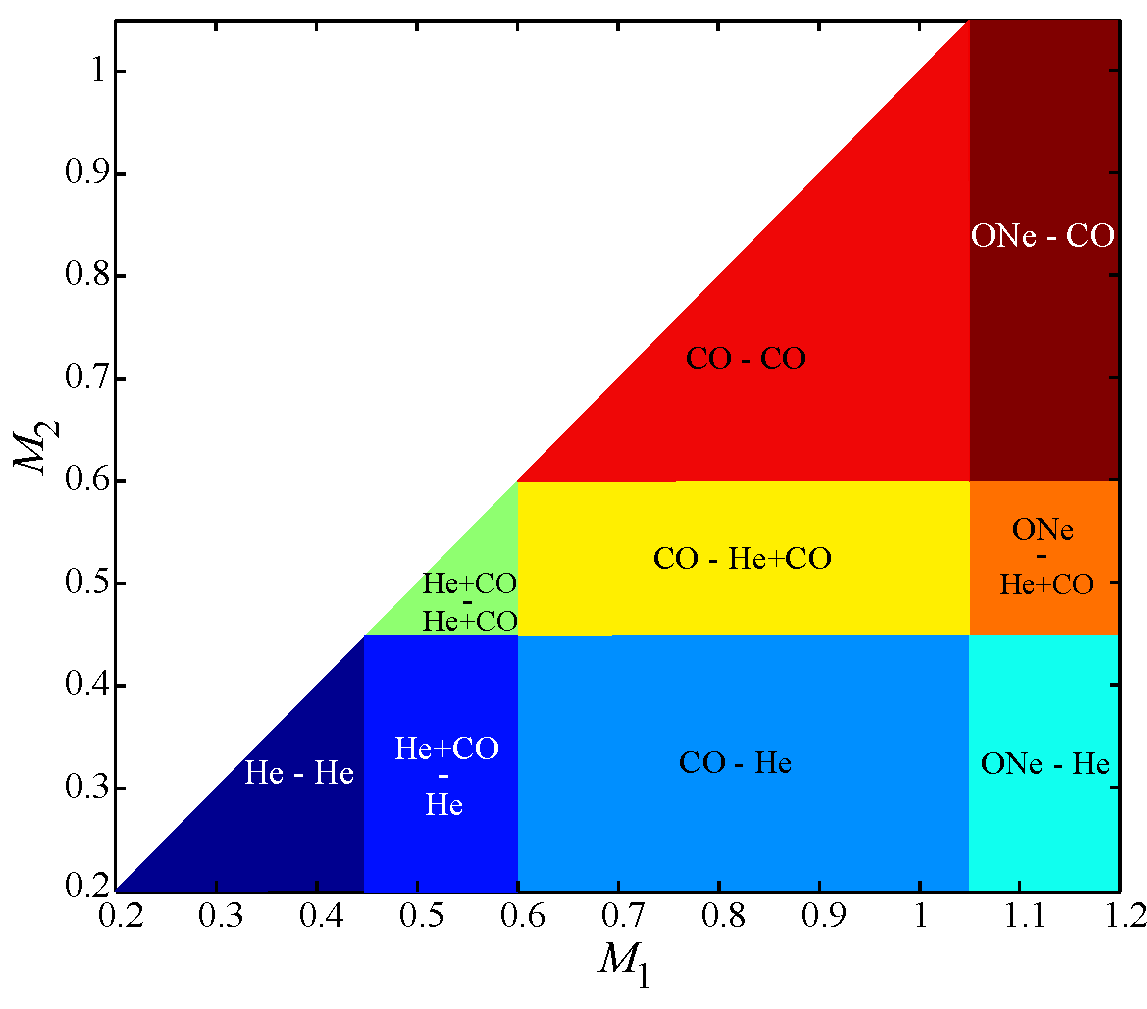
\includegraphics[width=0.6\hsize]{introduction/figures/dan+12_wdbinmass.pdf}
\caption{The expected compositions for white dwarfs undergoing a merger as a function of their masses, from \citeauthor{dan+12} (\citeyear{dan+12}, their Fig. 1).  $M_1$ is the mass of the accretor, or primary, WD (\Ma\ in the text), and $M_2$ is the mass of the donor, or secondary (\Md).  WDs with masses $M<0.45\,\Msun$ are assumed to be He WDs, those with $0.45 < M < 0.6\,\Msun$ CO WDs with thick He envelopes, $0.6 < M < 1.05\,\Msun$ CO WDs, and $M>1.05\,\Msun$ ONe WDs.  See text, as well as \cite{dan+12} Sec. 2, for discussion on these choices.}
\label{fig:c1_wdbinarymasses}
\end{figure}

% He flash - eg. \citealt{kippww12}, Ch. 33.4
% He WDs need friends: eg. \citealt{kippww12}, Ch. 33.4

The mass and composition of each WD within the binary is dependent on the binary's prior evolution.  Broadly speaking, WDs with masses $M \lesssim 0.45\,\Msun$ are composed of helium (He); these come from stars that had their evolution interrupted by binary interaction while on the red giant branch (eg. \citealt{marsdd95, nele+01, nele+01a}), before their degenerate He core became massive enough to trigger a helium flash.\footnote{He and CO WDs with $M\lesssim0.5\,\Msun$ could in principle come from single stellar evolution, but these take longer than a Hubble time to evolve.}  WDs with slightly higher masses have extensive He envelopes of $\sim0.1\,\Msun$ surrounding cores composed of carbon and oxygen (CO; \citealt{ibent85}).  \cite{dan+12} approximate the mass range of these ``hybrid WDs'' to be $0.45 \lesssim M \lesssim 0.6\,\Msun$, and set the composition of the upper $0.1\,\Msun$ of these WDs to He in their simulations.  From $0.6 \lesssim M \lesssim 1.1\,\Msun$ WDs are almost entirely composed of CO, with He atmospheres of $\sim10^{-2}\,\Msun$ \citep{ibent85}.  WDs with masses $\gtrsim 1.1\,\Msun$ come from super-AGB stars (eg. \citealt{herw05}) that ignite carbon during their evolution (eg. \citealt{garc13}), and thus are composed at least partly of oxygen and neon (ONe).  

Fig. \ref{fig:c1_wdbinarymasses}, from \cite{dan+12}, summarizes these relationships -- in it, $M_1$ is the mass of the more massive primary WD, which accretes mass during the merger, and $M_2$ is the mass of the secondary, which donates mass (see Sec. \ref{ssec:c1_stable_mass_transfer} for why this is always the case).  In this thesis, we refer to these as \Ma\ and \Md, respectively.  While sophisticated stellar evolution calculations are not always so clear-cut (eg. \citealt{ibent85, moros09} for CO WDs with $M\lesssim0.45\,\Msun$ and \citealt{hurlpt00} for CO WDs with $M\gtrsim1.2\,\Msun$), these relationships are used as rules of thumb for setting WD composition for a wide range of works (\citealt{loreig09,rask+12,dan+12,dan+14}, with slight variations between them).  In this thesis, we look at binaries of pure CO WDs (without He atmospheres) with masses ranging from $0.4 - 1.0\,\Msun$.

% for our parameter space study of mergers in Ch. \ref{ch:ch2}.  

%In subsequent chapters, we are primarily interested in the the merger of two CO WDs near the median mass of field WDs, $\sim0.65\,\Msun$ (Sec. \ref{ssec:c1_cowd_massrange}).

%The ratio of carbon and oxygen within CO WDs is also not particularly well-known.  In this thesis, we make the assumption that they are composed of 50\% carbon and 50\% oxygen by mass.  {\charles ADD STUFF}

%\subsection{Orbital Angular Momentum Loss and Gravitational Wave Emission}
%\label{ssec:c1_inspiral}

%magnetic braking ({\charles important for AM Canum Venaticorum systems} eg. \citealt{verb84, knigbp11})

Following their formation, WD binaries lose orbital angular momentum by emitting gravitational radiation (eg. \citealt{petem63}).\footnote{They may also lose angular momentum through the influence of a third body (eg. \citealt{katzd12}); see Sec. \ref{ssec:c1_new_typeia}.}  This loss has a characteristic inspiral timescale of \citep{segrcm97}

\begin{eqnarray}
\tau_{\mrm{grav}} = \frac{L_\mrm{orb}}{|\dot{L}_\mrm{orb}|} &=& \frac{5c^5}{32G^3}\frac{a^4}{\Ma\Md\Mtot}\nonumber \\
&=&5 \times 10^5 \left(\frac{a}{10^5 \mrm{km}}\right)^4 \frac{\Msun}{\Ma} \frac{\Msun}{\Md} \frac{\Msun}{\Mtot}\,\mrm{yr}.
\label{eq:c1_gravtimescale}
\end{eqnarray}

\noindent where $L_\mrm{orb}$ is the orbital angular momentum and $a$ is the orbital separation.  From this, we see that WD binaries with orbital periods on the order of hours or less ($a \lesssim 10^6\,\mrm{km} \sim 0.01\,\mrm{AU}$) will merge within a Hubble time.  

%It is estimated that there are on order of $10^8$ such systems in the Milky Way alone \citep{mars11, nele+01a}. <- This may be somewhat true, but don't write this unless you can guarantee all of these will merge within a hubble time!

As an aside, the gravitational waves emitted by inspiralling WD binaries are detectable from Earth.  With periods on the order of minutes, they are too low-frequency to be detected by Advanced LIGO \citep{ligo+15}, but are expected to be the most numerous and dominant source of gravitational waves \citep{mars11} detected by the proposed spaceborne detector eLISA (evolved Laser Interferometer Space Antenna; \citealt{amar+13}), which probes the mHz - Hz frequency range.  The instrument will likely resolve individual signals from thousands of binaries with orbital periods on the order $\sim10$ minutes (and are thus close to merging; \citealt{amar+13, mars11, dan+11}), while numerous sources that are too far away or at longer orbital periods will comprised an unresolved background \citep{neleyp01,amar+13}.  Measurement of either of these will probe the WD binary population of the Milky Way without the selection biases that often trouble electromagnetic binary searches \citep{mars11}.  Note that gravitational radiation plays a negligible role in the actual merger, as the waves released during the merger have a total energy $\sim10^{-10}$ of the binary's binding energy (eg. \citealt{loreig09}).

%Note, however, that final coalescence of the WDs is over far too quickly to be detectable by eLISA.

\section{Merger Outcomes}
\label{sec:c1_mergeroutcomes}

Like any merger, those between WDs liberate of order their gravitational binding energy.  This can lead to enough heating and/or compression to reignite the nuclear furnaces of normally inert WDs.  As this may happen under either non-degenerate or degenerate circumstances, the end product of such mergers are diverse, ranging from stars with unusual properties undergoing stable nuclear burning to explosions. Additionally, hydrostatic WDs have a maximum stable mass beyond which they are unstable to collapse -- the \cite{chan31} mass, or \Mch, at $\sim1.4\,\Msun$.  This has long led to the notion that sufficiently massive WD mergers can result in the complete destruction of the merger product in a thermonuclear explosion that would resemble a type Ia supernova (SN Ia; \citealt{webb84}), or in its transformation into a neutron star (NS) in an event known as an accretion-induced collapse \citep{nomoi85, saion85}.  We now know of a much greater range of possible merger outcomes for both systems with masses above and below \Mch.  Which outcome occurs depends on the compositions of the WDs involved, and are briefly summarized below (see also \citealt{dan+14}, who produce a similar list):

% dan+14 Fig 12, dan+12 fig 8

\begin{itemize}
	\item The merger of {\bf two He WDs} is unlikely to lead to violent nuclear burning and an explosion \citep{dan+12,dan+14,dan+15}.  Instead, merger remnants with total masses $0.4\lesssim \Mtot \lesssim 0.8$ \citep{han+02,ibent85}\footnote{This is lower than the He flash mass of $\sim0.45\,\Msun$ because the merger remnant is partly non-degenerate \citep{ibent85, han+02}.}, which are the vast majority of double He WD remnants \citep{nele10}, are expected to ignite He burning in a shell.  \citep{saioj00} and \cite{zhanj12} calculate that He shell burning increases the radius and luminosity of the star, turning it over $\sim 10^3-10^4\,\mrm{yr}$ into a yellow giant.  Over the next $10^5-10^6\mrm{yr}$, the burning shell migrates inward with a series of weakening shell flashes, while the radius slowly shrinks to $\sim10^{-1}\,\Rsun$.  Once the shell reaches the center of the remnant, it settles onto the helium main sequence, and resembles a He-rich subdwarf B (sdB) or O (sdO) star \citep{saioj00, justph11, zhanj12, hebe16}.  Most subdwarf stars are in binaries -- and likely arise from other formation channels -- and there are multiple proposed mechanisms to produce single sdB stars (such as a merger between a low-mass star or brown dwarf and a red giant; \citealt{soke98}), and so the contribution of mergers to the sdB population remains unclear \citep{nele10, hebe16}.

%"with properties similar to Extreme Helium (EHe) and R Coronae Borealis (R CrB) stars \citep{saioj00, zhanj12}", but this then makes the description too confusing.

% See conclusion section of hebe16 for alternate sources of single subdwarfs.  From hebe16: single sdBs tend to be narrowly peaked in mass, not obvious if mergers can do this.  Low mass MS star or brown dwarf may merge with RGB core to make single sdB in CE, He WD/MS merger.  From nele10: enhanced single star mass loss might do it too, but not obvious if this happens

%(\citealt{justph11}; He-poor sdO stars are likely evolved sdB stars)

	\item The outcome of a merger between {\bf an He and a CO WD}, or a merger between an He and hybrid He-CO WD, depends on whether or not a He explosion is touched off during the merger.  Roughly speaking, mergers with $\Mtot \lesssim 0.8\,\Msun$ will lead to steady He burning in a shell, and are thought to be the progenitors to He-rich sdO stars \citep{justph11}.  Mergers with $\Mtot \gtrsim 0.8\,\Msun$ that do not experience an explosion will also ignite shell burning, but unlike sdOB progenitors they will retain their extended envelope over the lifetime of the He-burning shell \citep{ibent85, zhanj12b}.  These mergers are believed to be the primary formation channel for Hydrogen-deficient Carbon (HdC) and R CrB stars (eg. \citealt{webb84, ibent84, saioj02, clay12, zhan+14}), which are H-deficient, He- and C-rich supergiants that, in the case of R CrB stars, feature abrupt variability by up to a factor of $\sim10^3$ due to the formation of carbon dust above their photospheres.\footnote{Subdwarf stars formed from double He WD mergers with $\Mtot \gtrsim 0.8\,\Msun$ will also expand to become R CrB stars following core He exhaustion, but this formation channel accounts for only a few percent of all R CrBs \citep{zhanj12b}.}  Following He shell exhaustion, they will contract in radius and heat their envelopes, resembling EHe stars \cite{saioj02, jeff14}.

Helium explosions become more likely for binaries with $\Mtot\gtrsim\Mch$ \citep{dan+12, dan+14}.  In cases where an accreted He shell explodes, but the underlying CO WD remains, the result depends on a number of factors including the mass of the CO WD and amount of He it accretes, and spans a wide range of possible peak luminosities \citep{woosk11}.  Detonations (or deflagrations; \citealt{woosk11}) of $\lesssim0.1\,\Msun$ He shells lead to explosions that reach peak brightnesses $\sim10-100$ fainter than SNe Ia over $\sim2-10$ days (typical SNe Ia values are in Sec. \ref{sec:c1_mysteryofsneia}), making them similar to the ``.Ia SNe'' theorized to occur in AM Canum Venaticorum binaries \citep{bild+07}.  They synthesize Ca, Cr and Ti, but relatively little of the radioactive \Ni\ typically seen in SNe Ia \citep{shen+10he, woosk11, wald+11}.  Denser He envelopes (due to it or the CO WD accretor being more massive), tend to synthesize more \Ni\ in detonations \citep{shen+10he, wald+11}. 

%As an aside, \cite{wald+11} also suggest that the detonation of $\sim0.2\,\Msun$ of He on top of a $\sim0.45\,\Msun$ CO WD could explain the SN 2005E-like class of low-luminosity SNe Ib that produce very little \Ni, have low ejecta masses and spectroscopically show strong lines of He, Ca and Ti \citep{pere+10}.  Their initial conditions (and those of \cite{shen+10he}) assume the He envelopes were constructed through slow ($\lesssim10^{-6}\,\Msun\,\pyr$) accretion onto the CO cores until He nuclear runaway is triggered through compressional heating.  Mergers between low-mass CO and He WDs will likely generate He envelopes that are far less degenerate, and which will not experience such a nuclear runaway.

% moreover simulations suggest He detonations in mergers occur before an He envelope of more than a few $10^{-2}\,\Msun$ can accrete onto the disk.

%Less degenerate material will lead to explosions dominated by lighter elements like Ca \citep{woosk11}, and therefore He detonation may be possible in really massive systems.  Dan+14 already had that idea though; see below.

In the case where the the He shell detonates, and triggers the CO WD to do the same, a ``double-detonation'' SN Ia may be produced (Sec. \ref{ssec:c1_new_typeia}).

	\item The merger of {\bf two CO WDs} has long been suspected of producing an SN Ia under the right conditions (Sec. \ref{sec:c1_mysteryofsneia} and \ref{sec:c1_vkchannel}).  If these conditions are not met, they will instead create a lone massive, rotating and highly magnetized CO WD or, if steady carbon fusion is ignited, a carbon-burning star that eventually turns into an ONe WD (Sec. \ref{sec:c1_hotdqs}).  If the ONe WD is above \Mch, it may collapse into a neutron star (see below).

	\item Due to their mass, it is likely that the merger of {\bf an ONe WD} with any companion will create a super-\Mch\ remnant.  Unlike their CO counterparts, an ONe WD that is compressed through accretion to $\gtrsim3\times10^9\,\gcc$ initiates electron-capture reactions onto $^{20}$Ne and $^{24}$Mg, losing degeneracy support in the process (eg. \citealt{miya+80, saion85, schwqb15}).  This leads to further contraction, which likely ends\footnote{Since the electron capture reactions are exothermic, they trigger a thermal runaway that eventually starts an O-deflagration at $\sim10^{10}\,\gcc$.  Whether or not collapse or explosion occurs depends on exactly when the deflagration ignites; see eg. discussion in \cite{schwqb15}.} in an ``accretion-induced collapse'' (AIC) into a neutron star soon after its central density reaches $\sim10^{10}\,\gcc$ \citep{schwqb15}.  Simulations \citep{dess+06, dess+07, frye+09} of the AIC find it expels only $\sim10^{-2}\,\Msun$ of ejecta and produces negligible amounts of radioactive \Ni, suggesting a very faint transient.

%Note - oxygen pycnonuclear fusion occurs well beyond 10^10 gcc (Fig. 12 Schw+15)

\cite{dan+14} discusses the possibility that He - ONe and CO - ONe WD mergers will lead to enshrouded AIC that produce ``hybrid supernovae'', where much of the outer envelope (of a different composition) explodes rather than collapsing.  In particular, they suggest (based on the \cite{shen+10he} and \cite{wald+11} simulations above) that the detonation of the thick He envelope of a significantly super-\Mch\ He - ONe WD merger remnant could  explain the SN 2005E-like class of low-luminosity SNe Ib that produce very little \Ni, have low ejecta masses and spectroscopically show strong lines of He, Ca and Ti \citep{pere+10}.

\cite{marq+15} suggest that an ONe WD could be detonated through binary interactions in the same manner as CO WDs (Sec. \ref{ssec:c1_new_typeia}).  Due to their high densities, these would produce $\gtrsim1\,\Msun$ of \Ni, but, because fusing to \Ni\ from O and Ne generates $\sim30$\% less energy than from C \citep{marq+15}, they would also be weaker than CO WD detonations.  Detonations during ONe mergers may explain supernovae such as SN 2009dc \citep{taub+09} that have a peak brightness $\sim3$ times higher, and decay from peak brightness $\sim3$ times more slowly, than SNe Ia, and also have low expansion velocities.

\end{itemize}

Of these possibilities, ones that create SNe Ia are particularly intriguing, as they may hold the key to solving the long-standing problem of how these explosions arise.

\section{The Mystery of Type Ia Supernovae}
\label{sec:c1_mysteryofsneia}

%It was only in the 20th century, however, that the they were recognized, through photometric and spectroscopic observations, as being a phenomena separate from novae \citep{baadz34}, and supernovae caused by the core-collapse of massive stars \citep{mink41, elias}.

Type Ia supernovae, or SNe Ia, have been observed by astronomers for centuries.  SN 1572, for example, was observed by Danish astronomer Tycho Brahe to be ``far beyond the Moon'', and helped lead to the abandonoment of the Aristotilian concept that the heavens were immutable \citep{ruiz04, krau+08}.

Today, SNe Ia are classified (eg. \citealt{fili97, li+11}) by the lack of hydrogen and helium, as well as the strong prescence of ionized silicon (Si II), in their spectra.  They are estimated to comprise a quarter of all supernovae in the local universe \citep{li+11}, but are found disproportionately often by surveys because most of their luminosity is emitted in the optical \citep{howe11}.  ``Normal'' SNe Ia \citep{bran98, bran+06} typically reach a maximum bolometric luminosity of $\sim10^{43}\,\ergpsec$ (see eg. \citep{fili97, hill+13}) after 18 - 20 days, followed by an order-of-magnitude decline in brightness over a month, and a slower, exponential decline of a factor of $\sim2.5$ every month (generally attributed to heat from radioactive decay within the ejecta).  Their spectroscopic features show they are composed of a combination of intermediate-mass elements (eg. \citealt{arne96}) such as silicon and calcium, and peak-iron elements such as iron and nickel \citep{fili97}; indeed they are the primary source of peak-iron elements for the galaxies that host them, and so play a crucial role in star formation and galactic chemical evolution \citep{leib00}.  Up to $\sim30$\% \citep{li+11} of explosions classified as SNe Ia are ``peculiar'' phenomena that are orders of magnitude fainter (eg. SN 2002cx \citep{li+02, fole+13}, SN 1991bg \citep{mazz+97}) and occassionally substantially brighter (eg. SN 2009dc; \citealt{yama+09, taub+09}).  Normal SNe Ia, however, are remarkably homogeneous, and exhibit variations that can -- to first order -- be parameterized by a single variable \citep{hilln00, howe11, maozns14}.  This is reflected most famously in the \cite{phil93} relation, where SNe Ia with greater peak brightnesses tend to evolve more slowly in time.  

Their parameterizability, as well as their intrinsic brightness, make SNe Ia outstanding cosmological distance indicators.  They were most famously used in this context in the much-celebrated discovery of \citep{ries+98} and \cite{perl+99} that the expansion of the universe is accelerating under the influence of a ``dark energy'', the exact nature of which remains mysterious.

Despite their ubiquity and utility, however, the exact nature (or natures) of their progenitor systems remains mysterious.  They were first proposed to be explosions of CO WDs by \citep{hoylf60} based on the composition of SNe Ia ejecta.  This is now well-established by the similarity of the light curve, energetics and spectrum of a typical SN Ia to those calculated for an exploding CO WD.  Also, early-time observations of the recent SN 2011fe have constrained the radius of the exploding object to be $\lesssim0.1\,\Rsun$ \citep{nuge+11, bloo+12, maozmn14}, consistent with a CO WD, and late-time observations of SN 2014J have detected gamma-ray emission from the decay of \Ni, produced by the burning of carbon and oxygen to nuclear statistical equilibrium, into stable $^{56}$Fe \citep{chur+14}.  What is much less well-understood is how the CO WD is made to explode, and a vast body of literature now exists exploring the various theoretical and observational lines of evidence.  For this reason, the references below are necessarily only a sample of the work currently being done; see \cite{howe11}, \cite{hill+13}, \cite{maozmn14}, and \cite{tsebs15} for excellent reviews and further references.

\subsection{Traditional Formation Scenarios and Their Pitfalls}
\label{ssec:c1_old_typeia}

Until recently, the most widely accepted progenitor scenarios have involved getting a CO WD to ignite by slowly adding mass to it \citep{hilln00}.  The added mass leads to compression and heating of its interior, but the latter is at least partly balanced by cooling from neutrino emissions, which prevents carbon ignition due to high temperatures.  As the CO WD approaches \Mch, its central density exceeds $\sim2\times10^9\,\gcc$, and the rate of heating from pycnonuclear carbon fusion -- i.e. carbon fusion due to extreme density -- exceeds that for neutrino cooling.  Because ignition occurs under highly degenerate conditions, the WD does not respond to this heating by expanding, and so, unlike a non-degenerate star, is unable to hydrodynamically regulate the nuclear reaction.  Instead, the WD experiences a runaway reaction that lasts $\sim1000\,\mrm{yr}$, until the timescale for nuclear burning at the WD's center becomes shorter than the star's dynamical time.  Dynamical burning then begins, and some kind of explosion becomes inevitable.

The various scenarios to get a CO WD to accrete slowly can subdivided into two classes, or ``channels'': the single-degenerate (SD) channel \citep{wheli73}, where the WD steadily accretes from a non-degenerate companion (a main sequence star, a giant, or a He-burning subdwarf; \citealt{maozmn14}), and the double-degenerate (DD) channel \citep{ibent84, webb84}, where two CO WDs with a total mass $\gtrsim\Mch$ merge, producing a merger remnant composed of a dense, degenerate ``core'' surrounded by a thick accretion disk.  Both scenarios are beset by a number of issues, which we summarize these below, following \citeauthor{vkercj10} (\citeyear{vkercj10}, henceforth \citeal{vkercj10}; see also \citealt{vker13}).

The first issue is that in order to match the observed SN Ia rate of $\sim 0.0023 \pm 0.0006$ for every solar mass of stars formed \citep{mann+05}, $\sim1$\% of all WDs formed (of any composition and regardless of binarity) must produce SNe Ia.  Compared to this relatively large number, there is an apparent paucity of CO WDs that can reach \Mch\ from either channel.  In hydrogen-accreting SD systems, efficient growth of the CO WD appears only achievable if the accretion rate is between $10^{-8} - 10^{-7}\,\Msun\,\pyr$.  Slower accretion results in nova outbusts that eject the accreted mass (\citealt{townsb04}; though see \citealt{zorosg11}), while faster accretion results in the buildup of an extended, red giant-like envelope that eventually engulfs the donor \citep{ibent84}.  Systems that do accrete at the correct rate -- and steadily burn hydrogen to helium -- should radiate supersoft x-rays, but observations of galactic x-ray flux suggest a factor of $10 - 100$ too few of these systems exist to explain the SNe Ia rate \citep{dist10, gilfb10}, and whether or not these systems can be ``hidden'' from view as rapidly-accreting enshrouded WDs is debateable (eg. \citealt{hachkn10, joha+14}).  Even if the accreted matter has been burned to helium, or the donor is He-rich, matter may still be ejected by subsequent helium flashes (\citealt{idanss13}; though see \citealt{hill+16}).  

Meanwhile, analytical estimates (\citealt{vkercj10}), binary population synthesis \citep{menn+10, ruitbf09, clae+14, maozns14} and empirical counting of candidate systems \citep{badem12} all estimate that the merger rate of CO - CO WD binaries with total mass greater than $\sim\Mch$ falls short of the SN Ia rate by a factor of at least a few.  Not all of these mergers will necessarily end as SNe Ia, either: if post-merger evolution leads to off-center carbon ignition in the merger remnant, it will transform the remnant into an ONe WD, and an $\gtrsim\Mch$ ONe WD ends its life in an AIC, rather than exploding as an SN Ia \citep{nomoi85, saion85, yoonpr07, schw+16}.
 
The second issue the difficulty for the thermonuclear explosion of an \Mch\ mass CO WD to replicate the properties of normal SNe Ia.  Normal SNe Ia synthesize $\sim0.5 - 1.3\,\Msun$ of radioactive \Ni\ (estimated from their bolometric light curves; eg \citealt{stri+06}), and feature absorption lines of intermediate-mass elements at maximum light, indicating that the explosion does not burn the entire WD to peak-iron elements, and lower-mass elements are preferentially located in the outer layers of the SN ejecta \citep{howe11, hill+13}.  If dynamical burning leads to an extended plateau of high overpressure a detonation \citep{seit+09} is triggered, where a supersonic shockwave drives through the WD and triggers nuclear fusion in its wake.  As most of the mass in an \Mch\ WD is $\gtrsim10^9\,\gcc$, a detonation would convert almost all of the WD to \Ni\ \citep{howe11, hill+13}.  On the other hand, if the explosion propagates as a subsonic deflagration, where a steep temperature gradient -- a flame front -- moves outward via conduction, the WD is able to expand during the explosion and, at lower densities, intermediate-mass elements are produced.  The explosion, however, produces slower velocity ejecta than seen in SNe Ia, and mixes burned and unburned material such that the ejecta do not appear stratified.  To resolve this, an \textit{ad-hoc} deflagration-to-detonation transition (DDT) is often invoked \citep{khok91}, the timing of which can be tuned to vary the amount of \Ni\ generated (eg. \citealt{hill+13}), though it remains to be seen this is a robust mechanism in realistic WD explosions (eg. \citealt{fishj15}).  It is also not obvious how invoking the DDT can explain the dependence of observed SNe Ia on the properties of their host galaxies, for example why more luminous SNe Ia tend to be in star-forming galaxies (eg. \citealt{hamu+00, howe+09, sull+10}).

The SD channel has a number of additional complications (and several others; see \citealt{maozns14, tsebs15}) that have led have the DD channel to fall into favor compared to the SD one.  For example, it requires a non-degenerate companion, which, under certain conditions, might be detectable, but attempts to spot the companion in pre-explosion archival data \citep{li+11cpn, nielvn13, niel+14}, during the supernova (as it responds to being hit by SN ejecta; \citealt{bloo+12,ollms15}), or after the explosion (eg. \citealt{kerz+14rem}).  For SD scenarios involving hydrogen-rich donors, the explosion is also expected to strip and entrain donor material, but attempts to find such material either do not detect hydrogen, or, in one recent case, apparently too little hydrogen to be consistent with SD donor stars \citep{magu+16}.  

%While these issues (and several others; see \citealt{maozns14}) have led the DD channel to fall into favor compared to the SD one, the issues discussed above affect \Mch\ progenitor scenarios in general.

% Mention gravitationally and pulsationally confined detonations??  Modern DDT: 2013MNRAS.429.1156S  GCD: http://adsabs.harvard.edu/abs/2016arXiv160600089S http://adsabs.harvard.edu/abs/2016ApJ...819..132G

\subsection{Brave New Channels}
\label{ssec:c1_new_typeia}

%In the following section, we will argue that the Chandrasekhar scenario shows significant problems when compared to observations of SNe Ia, and suggest that the majority of SNe Ia are caused by mergers of CO WD binaries, including those that produce remnants with masses below \Mch.  This argument is a summarization of the argument in \cite{vankerkwijk}.

The challenges posed by the evidence above has spurred research into alternative scenarios that lead to exploding CO WDs that are more physically viable and better fit observations.  Notably, several of these channels (highlighted below) relax the condition that the exploding WD must be at \Mch\ and allow for a range of exploding masses.  The alternate scenarios include:

\begin{itemize}

	\item The {\bf double-detonation channel} \citep{livn90, woosw94}, which involves a CO WD accreting a thin envelope from an He-rich source (a He star, merger with an He/hybrid WD, or even the He atmosphere of a CO WD).  At some point -- for slow ($\lesssim10^{-6}\,\Msun\,\pyr$; \citealt{bild+07}) accretion, when the base of the envelope becomes hot enough to ignite He burning; for mergers, when a hotspot in the accretion stream or envelope reaches conditions for detonation \citep{guil+10, rask+12, pakm+13} -- the He shell detonates, which then either drives compression waves that converge at the core of the CO WD to prompt a detonation, or launches one directly into it.  Either can trigger the secondary detonation of the CO WD (though the latter is perhaps more plausible; \citealt{mollw13}).  Traditionally, this has required massive He shells of $\gtrsim0.1\,\Msun$, but the detonation of these around a CO WD leads to significant production of \Ni, inconsistent with the stratified nature of SNe Ia ejecta (eg. \citealt{krom+10,woosk11}).  While the robustness and conditions most conducive to a double-detonation remains a field of active research (eg. \citealt{woosk11, holc+13, shenm14, shenb14, dan+15}), more recent work has suggested detonations of thin, $\lesssim0.05\,\Msun$ He shells in both stable accretion and mergers onto $\gtrsim1\,\Msun$ CO WDs may be possible \citep{woosk11, pakm+13, shenm14}, and that a CO detonation via converging shockwaves is likely as a result \citep{fink+10, mollw13, shenb14}.  Studies of pure detonations of bare sub-\Mch\ CO WDs with masses between $\sim1-1.15\,\Msun$ (eg. \citep{shig+92, sim+10}) show light curves and spectra that are in good agreement with normal SNe Ia (arguably as good or better than the agreement for other explosion models {\charles CITATION}), while the detonation of the much less massive He shell greatly reduces (but does not entirely eliminate) contamination from He shell nuclear ashes \citep{krom+10, hill+13}.

If the double-detonation channel is indeed physically plausible, it opens up a (somewhat narrow) range of WD masses beyond \Mch\ that can explode, and more naturally explains the explosion that requiren a deflagration-to-detonation transition.  Peak luminosity of the explosion is dependent on the mass of CO WD, which could naturally explain both the \cite{phil93} relation and the relationship between SN Ia luminosity and the age of its host stellar population (since lower-mass merger constituents take longer to form; \citealt{sim+10}).

	\item The {\bf violent merger channel} \citep{pakm+10}, which is a variant of the double-degenerate channel where, during the merging process, material being accreted from one WD to another is sufficiently superheated and compressed to trigger a detonation, destroying both stars.  This sidesteps the need for slow accretion following the merger.  Only those binaries where the primary WD is $\gtrsim0.9\,\Msun$ and the WD mass ratio is $\gtrsim0.8-0.9$ (\citealt{pakm+10, pakm+11, sato+16}, though see \citealt{dan+12}, which suggests a higher minimum primary WD of $\gtrsim1.0\,\Msun$) are violent enough to trigger a detonation, though the mass ratio criterion is reduced at higher primary masses \citep{sato+16}.  Mergers with primaries of $\gtrsim1.0\,\Msun$ produce explosions with \Ni\ yields consistent with normal or overluminous SNe Ia \citep{pakm+12, moll+14}.  Lower-mass systems produce ones that only synthesize $\sim0.1\,\Msun$ of \Ni, and are much redder and have much slower velocities than typical SNe Ia, but could resemble the subluminous SN 1991bg-like SNe Ia subclass \citep{lieb+93, pakm+10}.  Whether a CO detonation can robustly be triggered during a merger requires further study, but regardless, the CO WD binaries considered here are highly super-\Mch, and may be far too rare to explain the majority of SNe Ia \citep{badem12}.

	\item The {\bf direct collision channel}, in which two potentially sub-\Mch\ CO WDs collide, rather than merge, either because they are in a dense stellar environment (such as a globular cluster; \citealt{benzth89, loreig10}) or a hierarchical triple system \citep{katzd12} under the influence of the Kozai-Lidov mechanism \citep{koza62, lido62}.  Hydrodynamic simulations in \cite{kush+13}, \citep{garc+13} and \citep{dong+15} show that the impact of the the WDs leads to strong shocks that plow into both WDs and detonate them.  Explosion properties can be varied by changing impact parameter or the masses of the stars, with the collision of two $\sim0.6\,\Msun$ CO WDs is able to produce $\sim0.2-0.5\,\Msun$ of \Ni\ \citep{garc+13, kush+13}, consistent with normal SNe Ia.  A minority of WD reside in dense stellar environments, however, and only $\sim10-20$\% of stars are in triples, making it unlikely that this channel alone can reproduce a substantial fraction of SNe Ia (see Sec. 2.3 of \citealt{maozmn14} for details).

	\item The {\bf core-degenerate channel} \citep{livir03, kashs11, tsebs15}, which occurs when a progenitor system that would otherwise have produced a $>\Mch$ close-in double WD binary does \textit{not} survive its (second) common envelope phase (or survives in such a tight orbit that it merges within $10^6$ years afterward).  To account for most SNe Ia, the super-\Mch\ remnant would have to survive for $10^{8}-10^{10}\,\mrm{yr}$ before exploding (since SNe Ia can occur in stellar environments that have long ceased star formation; eg. \citealt{prichs08, maozsg10}).  \cite{illks12} proposes this can be done through a gradual loss of solid-body rotational support through magnetic dipole radiation, but this is not obviously physically robust (see post-merger evolution discussion in Ch. \ref{ch:ch2}).  Nonetheless, mergers during or just after common-envelope events naturally explain peculiar SNe Ia that show interaction with a large mass of circumstellar material (eg. PTF 11kx; \citealt{dild+12, soke13}).

\end{itemize}

More unconventional channels have also been proposed that allow a CO WD to detonate due to collisions with planets and planetoids \citep{distfg15} or even lone sub-\Mch\ WDs due to compositional impurities near their core that lower the density required for the onset of pycnonuclear fusion to $\gtrsim0.9\,\Msun$ \citep{chio+15}.  Further work is required to show the physical viability of these channels, and whether they reproduce normal SNe Ia.  

Regardless of whether or not any of these produce normal SNe Ia, study of these mechanisms is useful for explaining the diverse subclasses of SNe Ia.  Aside from the peculiar SNe listed above, synthetic light curves and spectra of pure deflagrations of \Mch\ CO WDs \citep{phil+07, krom+13, fink+14} reproduce the low peak brightness, slow ejecta velocity and hot photospheric emission of the SN IaX subclass (or SN 2002cx-like; \citealt{li+02, fole+13}).  Meanwhile, successful detonations of \Mch\ CO WDs have been linked to the overluminous SN 1991T-like SNe Ia (\citealt{fishj15}, but see \citealt{seit+16}).

%For one IaX, progenitor might have been found (2014Natur.512...54M), but no need to invoke bound remnant? (2015A&A...573A...2S)  Meanwhile, possible bound remnant found in another (2016MNRAS.tmp..977F).

\section{The vK10 SN Ia Channel}
\label{sec:c1_vkchannel}

Another alternate channel was recently proposed in \citeauthor{vkercj10} (\citeyear{vkercj10}; henceforth \citeal{vkercj10}), which considers the possibility that CO WD mergers with masses significantly below \Mch\ can also explode.  They consider a fiducial merger of a $0.6-0.6\,\Msun$ CO WD binary, whose masses are chosen to be near the empirical peak of the WD mass distribution (Sec. \ref{ssec:c1_cowd_massrange}).  Hydrodynamic simulations \citep{loreig09} find that the two WDs tidally destroy one another and coalesce into a remnant that is significantly heated throughout, but does not achieves temperatures sufficient to ignite fusion (as it is much less massive than the violent mergers considered in Sec. \ref{ssec:c1_new_typeia}); moreover, the remnant central density, $\sim2.5\times10^6\,\gcc$, is too low to produce \Ni\ in an explosion.  Following coalescence, however, the remnant, which is differentially rotating, enters a period of rapid angular momentum redistribution due to hydrodynamically or magnetically-mediated viscosity.  Using the standard $\alpha$-viscosity prescription \cite{shaks73} -- i.e. $\nu = \alpha c_s H_P$, where $c_s$ is the sound speed and $H_P$ the pressure scale height -- the timescale for viscous evolution can be estimated as

\begin{eqnarray}
t_\mrm{visc} &=& \frac{R_\mrm{disk}^2}{\nu} \sim \frac{1}{\alpha}\frac{R_\mrm{disk}^2}{H_P^2}\taudyn \nonumber \\
			&\sim& 3\times10^4\,\mrm{s}\left(\frac{10^{-2}}{\alpha}\right)\left(\frac{R_\mrm{disk}/H_P}{10}\right)^2\left(\frac{R_\mrm{disk}}{10^9\,\mrm{cm}}\right)^{3/2}\left(\frac{M_\mrm{enc}}{1\,\Msun}\right)^{-1/2},
\end{eqnarray}

\noindent where $M_\mrm{enc}$ is we have used $\taudyn \approx H_P/c_s$ and inserted a fiducial viscosity and typical numbers for remnants \citep{shen+12}.  Thus the vast majority of the remnant's angular momentum is transported away, and the remnant (including its disk) loses its rotational support against gravity, over a period $\sim10^4\,\mrm{s}$.\footnote{This is notably in contrast to earlier work (eg. \citep{nomoi85, yoonpr07}) that assume any rotationally-supported material will slowly accrete onto the dense core of the remnant at a near-Eddington mass accretion rate of $\dot{M} \sim 10^{-5}\,\Msun\,\pyr$.  Remnants are prone to magnetic instability \citep{shen+12,ji+13}, and will almost certainly evolve over the much shorter timescale given by the $\alpha$-viscosity estimate.}  This loss of rotational support combined with increasing weight from newly accreted disk material leads to compression and heating of the remnant core.  Since $\sim10^4\,\mrm{s}$ is far shorter than either the neutrino cooling timescale of $\taunu \sim 10^3\,\mrm{yr}$ or the thermal adjustment timescale of $\sim10^4\,\mrm{yr}$ \citep{shen+12}, compressional heating is adiabatic, and \citeal{vkercj10} estimates that for the $0.6-0.6\,\Msun$ remnant it leads both the central density and temperature to increase to $\gtrsim1.5\times10^7\,\gcc$ and $\gtrsim10^9\,\mrm{K}$, at which point the nuclear fusion timescale is smaller than even the compressional heating timescale, and a carbon nuclear runaway becomes inevitable.  If the runaway leads to dynamical burning and an explosion occurs, the generally lower densities of merger remnants compared to \Mch\ WDs (at $\sim3\times10^9\,\gcc$) means that burning leads to larger pressure differential between the ashes and their surroundings, perhaps making a detonation favorable over a deflagration (e.g. \citealt{mazumw77}; \citealt{seit+09}).

The \citeal{vkercj10} scenario features a number of advantages over the traditional \Mch\ double-degenerate channel.  Like the double-detonation channel, this one substantially increases the number of binary systems that could potentially explode -- perhaps by a factor of $\sim3$, which would be much more consistent with the SN Ia rate; \citeal{vkercj10}; \citealt{badem12} -- and naturally explains both the explosion mechanism and some of the trends seen in the observed SN Ia population, thus alleviating the issues discussed in Sec. \ref{ssec:c1_old_typeia}.  Unlike the double-detonation channel, however, a He detonation is not invoked to trigger the CO WD to explode -- negating the complications of the He detonation ashes on the SN light curve -- and the merger process perhaps provides a more natural means of producing the $\gtrsim1\,\Msun$ of CO needed to synthesize the \Ni\ found in a typical SN Ia (eg. \citealt{pirotk14}).

For this scenario to proceed as described, the merger remnant must be heated throughout its interior, which only occurs for mergers of nearly equal-mass binaries.  In a scenario where very unequal masses merge, the less massive secondary WD is completely disrupted and forms a disk and envelope around a largely undisturbed primary \citep{loreig09}.  Carbon ignition is then likely to occur off-center, which could lead to stable carbon burning rather than an explosion (eg. \citealt{yoonpr07, shen+12}).

\section{Massive Merger Remnants}
\label{sec:c1_hotdqs}

If the remnant of a double CO WD merger is not eventually destroyed in an explosion, it will live on as a single, massive, rapidly rotating and likely magnetized WD.  If off-center carbon burning is ignited, the WD will be transmuted into an ONe WD over $\sim10^4\,\mrm{yr}$ \citep{nomoi85, shen+12} but will never collapse into a neutron star, since its mass is below \Mch.

%The mass of a WD can be observationally determined by combining spectroscopically determined effective temperature $T_\mrm{eff}$ and logarithmic gravitational acceleration $log(g)$ with a theoretical WD mass-radius relation (eg. \citealt{klei+13}).  \cite{klei+13} and \cite{trem+16} determine the masses of single non-magnetic DA WDs from the the 

%non-magnetic (DA spectral type) CO WDs 

A number of studies of the observed mass distribution of field WDs from sky surveys (eg. \citealt{liebbh05, giambd12, klei+13, reba+15a, reba+15b}) note a high-mass peak near $\sim1\,\Msun$ that is substantially offset from the global peak of the mass distribution at $\sim0.65\,\Msun$ (Sec. \ref{ssec:c1_cowd_massrange}), which could be evidence of a population of merger remnants.  This interpretation is controversial, however: a kinematic study of objects in this peak suggest they are singly evolved \citep{weggp12}, while population synthesis studies \citep{reba+15a, reba+15b, trem+16} give conflicting results as to whether there are more massive WDs than can be explained by single star evolution.  Moreover, theoretical and observational estimates of the merger rate (eg. \citep{badem12, toonnp12}) are too low to contribute the majority of systems in the high-mass peak (\citealt{giambd12, reba+15b, trem+16}; though this could just mean the estimates are incorrect).  Studies targeting ``high-field magnetic WDs'' (HFMWDs; \citealt{kawk+07, kepl+13, garc+16}), which possess fields of $B \gtrsim1\,\mrm{MG}$, suggest the population's mass distribution has a mean of $\sim0.8\,\Msun$, and overall does not resemble the low- and non-magnetic WD ones.  The origin of these WDs, though, remains debated \citep{brig+15, garc+16}, and it is possible the fields are a vestige of single-star (eg. \citealt{wickf05, kisst15}) or binary evolution prior to the WD's formation \citep{brig+15}.  

The most massive ($\gtrsim1.1\,\Msun$) and most highly magnetized ($\gtrsim10^9\,\mrm{G}$) HFMWDs are more likely to be WD merger remnants \citep{garc+12, kule+13, wicktf14}.  Among these is the often-cited RE J 0317-853 \citep{bars+95, kube+10}, a $\gtrsim1.3\,\Msun$ CO or ONe WD with extremely high temperatures of $\gtrsim3\times10^4\,\mrm{K}$, $700\,\mrm{ms}$ spin period and field strength of $B\sim10^8\,\mrm{G}$.  Others include PG 1658+440, with a mass of $\sim1.3\,\Msun$, magnetic field of $\sim10^6\,\mrm{G}$ and rotational period of $\sim6\,\mrm{hr}$, and SDSS J085523.87, with a mass of $\sim1.1\,\Msun$ and a field of $\sim10^7\,\mrm{G}$ (\citealt{ferrdg15}, and references therein).  There is ambiguity regarding these objects' origins as well, however: RE J 0317 is in a wide (non-interacting) binary with a $\sim0.85\,\Msun$ companion, and \cite{kule+10} showed that the cooling age of both WDs is approximately the same as that of its companion.  This, they claim, makes it unlikely for RE J 0317 to have formed either from single star evolution (since it should have become a WD before its companion) or a merger (since one of its two merger constituents must be $\lesssim0.7\,\Msun$ and would have become a WD after the companion).  It is also curious that all the objects mentioned above are DA WDs and show hydrogen in their spectra, which is unlikely to survive mergers due to the high temperatures achieved in them.

An interesting recent discovery

(eg. \citealt{dunlc15}), Dunlap and Clements in preparation)

%Sloan Digital Sky Survey \citep{york+00} Data Release 7 (SDSS DR7)


%http://adsabs.harvard.edu/abs/2016ApJ...817...27W


\section{Thesis Overview}

If sub-\Mch\ double CO WD mergers can either eventually explode or leave behind isolated massive CO/ONe WDs, which fate is preferred, and does that fate depend on the masses of the two WDs?  Can these mergers, as \citeal{vkercj10} claims, serve as a novel SNe Ia progenitor channel that naturally satisfies both explosion, rates and properties?  To answer these questions, we must put the \citeal{vkercj10} scenario under scrutiny, and understand the parameter space of possible merger remnants produced by double CO WDs -- in particular the fraction of them that have temperatures close to carbon ignition under highly degenerate conditions, how the subsequent viscous phase proceeds in detail, and whether carbon ignition in a remnant can lead to an explosion.  This thesis attempts to shed light on some of these issues through a series of theoretical studies utilizing both semi-analytical calculations and hydrodynamic and magnetohydrodynamic computer simulations.

%Thus, the \citeal{vkercj10} channel is both attractive for its many advantages and plausible given the order-of-magnitude estimates above.  Investigating whether these estimates hold under detailed scrutiny, and to determine which, if any, systems in the CO WD binary parameter space could follow the channel, is the purpose of this PhD thesis.

In Chapter \ref{ch:ch2}, I perform a battery of 3D hydrodynamics simulations of merging CO WD binaries with the smoothed-particle hydrodynamics code \gasoline\ in order to characterize the range of possible merger remnant configurations.  In particular, I discern which mergers are ``similar in mass'', and produce remnants that are substantially heated and rotationally supported throughout.  As discussed in Sec. \ref{sec:c1_vkchannel}, these are potentially SN Ia progenitor candidates via the \citeal{vkercj10} channel.  I also make simple estimates of the compressional heating the remnants will experience during post-merger evolution to determine which of them could eventually ignite carbon fusion.

The smoothed-particle hydrodynamics method is used by almost all simulations of WD mergers.  In Chapter \ref{ch:ch3}, I investigate whether the outcome of a merger simulation depends on its hydrodynamic scheme by performing a merger of a $0.625 - 0.65\,\Msun$ CO WD binary using either \gasoline\ or the moving-mesh magnetohydrodynamics code \arepo, and discover novel phenomena during the earliest phase of post-merger evolution.  I also detail work that led to a number of improvements in \arepo\ to prevent spurious loss of global angular momentum when simulating differentially rotating systems.

In Chapter \ref{ch:ch4}, I use \arepo\ to simulate the evolution of initially weak magnetic fields within the $0.625 - 0.65\,\Msun$ merger.  I find exponential field growth during the coalescence of the WDs that leads to a powerful, $>10^{10}$ G magnetic field in the merger remnant that could affect its subsequent evolution.

Lastly, in Chapter \ref{ch:ch5}, I consider the evolution of (idealized and quasi-hydrostatic) sub-\Mch\ CO WDs experiencing a nuclear runaway at their centers.  While, as stated in Sec. \ref{ssec:c1_old_typeia}, such a runaway inevitably leads to some form of explosion for \Mch\ WDs, in sub-\Mch\ ones it may instead lead to the lifting of degeneracy and expansion into a carbon-burning star.  I use analytical arguments and simple models to determine that the minimum mass required for the runaway to produce an explosion, and discuss the consequences my findings have on merger remnants after their viscous evolution.

Chapters \ref{ch:ch2} and \ref{ch:ch4} have been published as \cite{zhu+13} and \cite{zhu+15}, respectively, and Chapter \ref{ch:ch5} is being published simultaneous to the submission of this thesis.  For the most part, I have reproduced exactly the texts from each paper, only modifying the chapter introductions to prevent repetitious discussion of WD mergers and the \citeal{vkercj10} channel.  I have added postscripts to Chapters \ref{ch:ch2} and \ref{ch:ch4} that discuss their results in light of developments after their publication, and included an extensive appendix to Chapter \ref{ch:ch5} that details our calculation of convective suppression in magnetized, rotating WDs.  Any additional changes are noted at the start of each chapter.


\section{Thesis Overview}

The chapters are ordered in accordance with the proposed evolution of the \citeal{vkercj10} channel.  In Chapter \ref{ch:ch2}, we consider the range of possible merger remnant configurations to arise from the parameter space of merging CO WD binaries.  In 

For the most part, I have reproduced exactly the texts of \citeal{zhu+13}, \citeal{zhu+15} and \citeal{zhu+16} in their respective chapters.  The exceptions are the chapter introductions, where I have excised certain paragraphs to eliminate the redundancy of having multiple paragraphs repeating an overview of the \citeal{vkercj10} channel.  The papers' abstracts have also been modified into chapter overviews, and certain figures reformatted for readability.  Any additional changes are noted at the start of each chapter.  Most prominently, we have added a postscript to Chapter \ref{ch:ch2} (Sec. \ref{sec:postscript_pme}) that considers our simple semi-analytical prescription for post-merger viscous evolution in light of new results, and we included an extensive appendix to Chapter \ref{ch:ch5} that details our calculation of convective suppression in magnetized, rotating WDs.

\section{The Physics of Pre-Merger Evolution}

To preface Chapter \ref{ch:ch2}, which focuses on the merger remnants, we briefly cover a few topics related to evolution of the CO WD binary leading up to mass transfer, and the early stages of mass transfer leading up to the merger proper (which we refer to as ``coalescence'').

\subsection{Stable and Unstable Mass Transfer}

In Chapter \ref{ch:ch2}, every single one of our simulated binaries merge, as we use approximate initial conditions that place unperturbed, spherical WDs at separations that guarantee immediate Roche lobe overflow.  An order of magnitude estimate, however, would suggest that binaries with sufficiently small mass ratios would not merge at all.

%http://adsabs.harvard.edu/abs/2016arXiv160404269B
%http://adsabs.harvard.edu/abs/2015ApJ...805L...6S

\subsection{Are Merging WDs Co-Rotating?}

While this question is something that we shall discuss at length in Ch. \ref{ch:ch2} (and is also considered in other works such as \cite{XXX} and \cite{ji+13}) the results of Ch. \ref{ch:ch3} suggest that it is likely unimportant for the configuration of the merger remnant (at least to first order).

Check Schwab+12 intro for synchronization links.


%http://adsabs.harvard.edu/abs/2015ApJ...815...63A
%http://adsabs.harvard.edu/abs/2016ApJ...824...46B
%https://arxiv.org/abs/1606.05292

%http://adsabs.harvard.edu/abs/2015arXiv151203442P
%http://adsabs.harvard.edu/abs/2016MNRAS.tmp..977F



%http://adsabs.harvard.edu/abs/2016ApJ...817...27W

%http://adsabs.harvard.edu/abs/2016ApJ...818...26D

%http://adsabs.harvard.edu/abs/2016arXiv160401021F
%http://adsabs.harvard.edu/abs/2016ApJ...818L..19M

%ch2
\chapter{A Parameter-Space Study of Carbon-Oxygen White Dwarf Mergers}
\label{ch:ch2}

\begin{center}
\begin{minipage}[c]{4.75in}
Chenchong Zhu, Philip Chang, Marten H. van Kerkwijk and James Wadsley\\
The Astrophysical Journal, Volume 767, Issue 2 - article id. 164, 32 pp., 2013 \citep{zhu+13}
\vspace{2em}
\end{minipage}
\end{center}

As we discussed in Sec. \ref{sec:c1_vkchannel} and \ref{sec:c1_hotdqs}, the merger of two carbon-oxygen white dwarfs can lead either to a spectacular transient, stable nuclear burning or a massive, rapidly rotating white dwarf.  Previous simulations of mergers have shown that the outcome strongly depends on whether the white dwarfs are similar or dissimilar in mass \citep{loreig09}.  In the similar-mass case, both white dwarfs merge fully and the remnant is hot throughout, while in the dissimilar case, the more massive, denser white dwarf remains cold and essentially intact, with the disrupted lower mass one wrapped around it in a hot envelope and disk.

In order to determine what constitutes ``similar in mass'' and more generally how the properties of the merger remnant depend on the input masses, we simulated unsynchronized carbon-oxygen white dwarf mergers for a large range of masses using smoothed-particle hydrodynamics.  We find that the structure of the merger remnant varies smoothly as a function of the ratio of the central densities of the two white dwarfs.  A density ratio of 0.6 approximately separates similar and dissimilar mass mergers.  Confirming previous work, we find that the temperatures of most merger remnants are not high enough to immediately ignite carbon fusion.  During subsequent viscous evolution, however, the interior will likely be compressed and heated as the disk accretes and the remnant spins down.  We find from simple estimates that this evolution can lead to ignition for many remnants.  For similar-mass mergers, this would likely occur under sufficiently degenerate conditions that a thermonuclear runaway would ensue.

Aside from redundant parts of the introduction, we also do not reproduce here the extensive Appendix to \cite{zhu+13}, which contains tables of binary input parameters and remnant properties for the simulations, and its online figure set, depiciting merger remnant properties for all of our simulations.

\section{Introduction}
\label{sec:c2_intro}

Until recent years, efforts to find SN Ia progenitors among merging CO WD binaries have focused on those with total mass $M>\Mch$.  The end result of such mergers is believed to be either stable off-center carbon ignition, which would turn the merger remnant into an oxygen-neon WD and possibly eventually result in accretion-induced collapse \citep{saion98}, or slow accretion, which allows the remnant to stay cool and eventually ignite at high central density \citep{yoonpr07}.  Less massive mergers were usually thought to result in more massive, rapidly rotating CO WDs \citep{segrcm97,kube+10}, but more recently it has been realized these might eventually become hot enough to ignite (\citealt{vkercj10}, \citeal{vkercj10} hereafter; \citealt{shen+12,schw+12}).  Indeed, \citeal{vkercj10} argue that type Ia supernovae result generally from mergers of CO WDs with similar masses, independent of whether or not their total mass exceeds \Mch.  For all these studies, the conclusions on whether and where ignition takes place depend critically on the structure of the merger remnnant.

The merging process, and the merger remnant, have been studied quite extensively, mostly using smoothed-particle hydrodynamics (SPH; e.g. \citealt{mona05}).  These simulations have shown that the outcome strongly depends on whether the WDs are similar or dissimilar in mass.  In the similar-mass case, both WDs disrupt fully and the remnant is hot throughout, while in the dissimilar case, the more massive, denser WD remains essentially intact and relatively cold, with the disrupted lower mass one wrapped around it in a hot envelope and disk.  Less clear, however, is what constitutes ``similar-mass,'' and, more generally, how the merger remnant properties depend on the initial conditions.  

In principle, for cold WDs of given composition, the remnant properties should depend mostly on the two WD masses, with a second-order effect due to rotation.  In this paper, we try to determine these dependencies using simulations of WD mergers with the Gasoline SPH code, covering the entire range of possible donor and accretor masses, but limiting ourselves to non-rotating WDs.  Our primary aim is to identify trends between mergers of different masses, both to guide analytical understanding and to help scale other, perhaps more precise simulations.  Here, our hope is that while the results of individual simulations may suffer from uncertainties related to the precise techniques and assumptions used, the trends should be more robust.  We also try to provide sufficient quantitative detail on the properties of merger remnants that it becomes possible to make analytical estimates or construct reasonable numerical approximations without having to run new simulations.

Our work is complementary to the recent surveys of remnant properties by \cite{rask+12} and \cite{dan+12}, in that they focus on different scientific questions (e.g., orbital stability; possible detonation).  In contrast to our work, they assume that the WDs are co-rotating with the orbit.  Whether this is a better assumption than no rotation depends on the strength of tidal dissipation, which unfortunately is not yet known (see \citealt{marsns04,fulll12}).

This chapter is organised as follows.  In Section~\ref{sec:c2_gasoline}, we describe the SPH code we used, as well as our initial conditions.  In Section~\ref{sec:c2_results}, we present our results and give trends for a number of pertinent remnant properties.  In Section~\ref{sec:c2_variation}, we test the robustness of our results, and in Section~\ref{sec:c2_compwithothers} compare our results with those of \citeal{loreig09} and others.  Lastly, in Section~\ref{sec:c2_postmerger}, we speculate on the further evolution of our remnants, considering in particular whether, as suggested by \citeal{vkercj10}, some might lead to type Ia supernovae.

\section{Code and Input Physics}
\label{sec:c2_gasoline}

We simulate the mergers by placing non-rotating white dwarfs in a circular orbit with an initial separation {\azero} chosen such that rapid mass transfer begins immediately.  We then follow the merger for six orbits, at which time the remnant has become approximately axisymmetric.  As in prior work, the morphology of all merger remnants is similar, consisting of a dense, primarily degeneracy-supported center surrounded by a partly thermally-supported hot envelope (called a ``corona'' by \citeal{loreig09}) and a thick, sub-Keplerian disk.  We will use the terms ``core'', ``envelope'' and ``disk'' throughout this work.  We also quite often refer to both the core and envelope simultaneously as the ``core-envelope''.

We use simulation techniques and initial conditions that are standard in the field of WD merger simulations, both in order to compare with previous work, as well as to not introduce novel numerical effects into our simulations.  We detail our code and initial conditions below so that they can easily be reproduced.

\subsection{The SPH Code}
\label{ssec:c2_sphcode}

With smoothed-particle hydrodynamics, one uses particles as a set of interpolation points to determine continuum values of the fluid and model its dynamics.  SPH is a Lagrangian method, meaning movement is automatically tracked, and regions of high density contain more particles and therefore are automatically more resolved.  Moreover, SPH inherently conserves angular momentum in three dimensions, which is difficult to reproduce in grid codes except under specific coordinate systems and symmetries.  SPH therefore allows one to efficiently simulate complex phenomena with a large range of lengthscales.  It has become the method of choice for merger simulations, and so we chose it as well.

%In contrast, grid-based methods model bulk movement through numerically diffusive cell-to-cell transfer, and require adaptive meshes to follow density contrasts (difficult to implement for merging stars, where high density regions are constantly moving).

For our simulations, we use Gasoline \citep{wadssq04}, a modular tree-based SPH code that was designed and has been used for a wide range of astrophysical scenarios, from galaxy interactions to planet formation.  It aims for tight controls on force accuracy and integration errors.  Gasoline implements the \cite{hernk89} kernel -- we use 100 neighbors -- and uses the asymmetric energy formulation (\citeauthor{wadssq04}, Eqn. 8) to evolve particle internal energy.  In our simulations, total energy is on average conserved to 0.3\%, and angular momentum to 0.006\%.

By default, Gasoline uses the usual Monaghan and Gingold formulation for artificial viscosity (see \citealt{mona05}), together with a Balsara switch (a standard feature of WD merger SPH simulations) to reduce viscosity in non-shocking, shearing flows.  \cite{guerig04} found that such a prescription did not reduce viscosity sufficiently, resulting in excess spin-up of the remnant core and associated shear heating.  \cite{yoonpr07}, in addition to a Balsara switch, used variable coefficients for the linear and quadratic viscosity terms in the SPH equations of motion and energy, setting these values to $\alpha\,=0.05$ and $\beta\,=0.1$, respectively, where shocks are absent, and around unity where they are present.  A similar formulation was used in \cite{dan+11,dan+12}.  Since Gasoline includes it as well, we have used it for our study.  Excess viscosity nevertheless remains a potential problem;  we investigate its effects further in Sec.~\ref{ssec:c2_viscprescrip}.

We modified Gasoline to include support for degenerate gas through the Helmholtz equation of state (EOS)\footnote{Available at \url{http://cococubed.asu.edu/} .} \citep{timms00}.  This code, also used in \cite{rask+12} and \cite{dan+12}'s simulations, interpolates the Helmholtz free energy of the electron-positron plasma, along with analytical expressions for ions and photons, to determine pressure, energy and other properties from density and temperature.  It is fast, spans a large range of density and temperature, and has, by construction, perfect thermodynamic consistency.  To obtain quantities as a function of density and internal energy, we utilized a Newton-Raphson inverter.  To keep the energy-temperature relation positive-definite, we did not disable Coulomb corrections in cases where total entropy became negative.

%To obtain quantities as a function of density and internal energy, we utilized a Newton-Raphson inverter, disabling Coulomb corrections to keep the energy-temperature relation positive-definite.

Gasoline keeps track of the internal energy of particles, using it to determine other thermodynamic properties for fluid evolution.  A particle's energy will naturally fluctuate due to noise, but for nearly zero-temperature particles this could result in their energy dipping below the Fermi energy.  In such situations we keep the pressure at the Fermi pressure, while letting the energy freely evolve.  A consequence of the floor is that a small amount of excess energy is injected into the system through mechanical work, which eventually manifests as additional thermal energy.  The accumulated energy over a simulation is typically a small fraction of the internal energy, and therefore does not significantly affect the dynamics of the merger or most properties of the remnant.  In cold, degeneracy-dominated material, however, a small change in internal energy corresponds to a large temperature change, at times comparable to the physically expected values, and thus the temperatures near the centers of some of our simulations have been affected.  We characterize this spurious heating in Sec.~\ref{ssec:c2_spheat} and show that it does not unduly affect our work's conclusions.  However, it makes it difficult to run much longer simulations.

We also place an energy floor at half the Fermi energy.  This is to prevent particle energies from approaching zero (and consequently calling for tiny timesteps), which under rare circumstances occurs when particles perform a great deal of mechanical work.  We find this happens primarily for particles that are flung out of the system by the merger and are cooling rapidly, and therefore are confident it has only a very minor effect on our simulations.

%%%%%%%%%%%%%%%%%%%%%%%%%VS 2%%%%%%%%%%%%%%%%%%%%%%%%%%%%%%%%%

%A problem we encountered in modeling degenerate material is that a particle's energy can drift below the Fermi energy due to a ubiquitous noise source in SPH simulations: particles moving randomly at a small fraction of the speed of sound (e.g., \citealt{spri10rev}).  To prevent pressure from becoming unphysical, we do not let it decrease below its zero-temperature value.  We leave the internal energy as is to maintain energy conservation, except we do not let it decrease below half the Fermi energy.  The latter is to prevent particle energies from reaching below zero, which under rare circumstances appears to happen when particles perform a great deal of mechanical work.  We found this occurs primarily for particles that are flung out of the system by the merger and are cooling rapidly, and therefore are confident it has only a very minor effect on our simulations.

%A consequence of this pressure and energy floor is that a small amount of additional energy is injected into the system, which eventually manifests as additional thermal energy.  This spurious thermal energy is typically a small fraction of the internal energy, but since in our systems degeneracy pressure dominates, the small fraction correspond to a large temperature change, at times comparable to the physically expected values.  We characterize this ``spurious heating'' in Sec.~\ref{ssec:c2_spheat} and show that it does not unduly affect our work's conclusions.  However, it makes it difficult to run much longer simulations.

%%%%%%%%%%%%%%%%%%%%%%%%%VS 1%%%%%%%%%%%%%%%%%%%%%%%%%%%%%%%%%

%\footnote{Coulomb corrections are important only at high density and low temperature, and their removal would have very minor effects for our work.}

%A problem we encountered in modeling degenerate material is that it is affected much more strongly by a ubiquitous noise source in SPH simulations: particles moving randomly at a small fraction of the speed of sound (e.g., \citealt{spri10rev}).  Artificial viscosity helps damp this noise, but generates corresponding thermal energy.  This spurious thermal energy is typically a small fraction of the internal energy, and therefore if the pressure support is predominantly from thermal pressure changes to the temperature are negligible.  In our systems, however, degeneracy pressure dominates, and the small changes in internal energy correspond to large temperature changes, at times comparable to the physically expected values.  We characterize this ``spurious heating'' in Sec.~\ref{ssec:c2_spheat} and show that it does not unduly affect our work's conclusions.  However, it makes it difficult to run much longer simulations.

%because density and energy in Gasoline are not updated simultaneously

%Another issue we encountered is that a particle's energy can drift below the Fermi energy.  To prevent pressure from becoming unphysical, we do not let it decrease below its zero-temperature value.  We leave the energy as is to maintain energy conservation, except we do not let it decrease below half the Fermi energy.  The latter is to prevent particle energies from reaching below zero, which under rare circumstances appears to happen when particles perform a great deal of mechanical work.  We found this occurs primarily for particles that are flung out of the system by the merger and are cooling rapidly, and therefore are confident it has only a very minor effect on our simulations.


%%%%%%%%%%%%%%%%%%%%%%%%%%%%%%%%%%%%%%%%%%%%%%%%%%%%%%%%%%%%%%

%partly because we hoped our simulations could guide analytical understanding of mergers, and hence we wanted to avoid complications, and also

In our work, we ignore outer hydrogen and helium layers, composition gradients, and any nuclear reactions.  This is mainly because previous work has found that nuclear processing was unimportant during the merger.  For instance, \citetalias{loreig09} found fusion released $\sim\!10^{41}$ erg for their 0.6 - 0.8 {\Msun} merger, orders of magnitude smaller than the $\sim\!10^{50}\,$erg binding energy of the remnant.  Only for mergers involving very massive, $\gtrsim\!0.9\,M_\odot$ WDs might this assumption break down, with the possibility of carbon detonations arising (\citealt{pakm+10,pakm+11,pakm+12}; but see \citealt{rask+12,dan+12}).  Similarly, \cite{rask+12}, who included standard helium envelopes of $\sim\!1-2$\% of the WD mass in their simulations, found that only for accretors with masses above $\sim\!1\,\Msun$ did it make a substantial difference: a helium detonation would inject $\sim\!10^{49}\,$erg into the merger remnant.  While this led to additional heating, it was insufficient to trigger much carbon burning or unbind any portion of the remnant (helium detonations have also been found for lower-mass accretors with CO-He hybrid donors; \citealt{dan+12}).

%As previous works \citep{guerig04,yoonpr07,loreig09} have discussed, most CO WD mergers do not experience nuclear runaways during the course of the merger.  While some nuclear processing occurs, the timescale associated with the heating is far longer than the merger timescale, which is typically a few dynamical times \citep{guerig04,loreig09}. Only the most massive mergers can experience nuclear burning on merger timescales.  In these cases, detonations are triggered in the helium atmospheres of the merging WDs or in the carbon interior if the merger is sufficiently violent.  For instance, \citeauthor{rask+12} showed that, for a 0.96 - 1.06 {\Msun} merger, the He detonation burns the majority of surface He in the merging WDs, and injects some $10^{49}$ erg into the merger.  However, this was not sufficiently energetic to trigger significant carbon burning or unbind the star.  In another study of surface He detonations, \citeauthor{dan+12} have found potential He surface detonations for a large range of accretors provided that the donor has a thick He shell and a total mass greater than $\sim 45$ {\Msun} {\bf CHARLES: CHECK THIS NUMBER}.  Only the most massive mergers ($M_\mathrm{tot}\,\gtrsim\,1.8$ {\Msun}) may experience carbon detonations \citep{pakm+10,pakm+11,pakm+12}.  However these detonations occur while the WD has not yet dynamically relax and retains it initial central density.  The resulting detonation usually does not produce sufficient iron group elements and produces a subluminous SN Ia.  Only for the most massive system does a normal SN Ia result.  Because the primary aim of this study is to consider the parameter space of WD mergers as a whole, the majority of which do not experience nuclear burning, we will assume that none of the systems we consider detonate during the merger.

%\citet{pakm+10,pakm+11,pakm+12} found carbon detonations occurring during (rather than after) the merger of nearly equal mass WD pairs with total mass $\gtrsim\,1.8$ {\Msun}.  These detonations occur while the WD has not yet dynamically relaxed and therefore retains its initial central density.  They therefore do not produce sufficient iron group elements and resemble subluminous SNe Ia.  Only for the most massive systems does a normal SN Ia result.  Moreover, whether or not conditions for detonation are actually reached in these simulations is controversial (see discussion in \citeauthor{rask+12} and \citealt{dan+12}).  In ignoring nuclear reactions, we proceed with the possibility that the most massive mergers in our parameter space may be too cold and degenerate, or may have already exploded.

\subsection{Initial Conditions}
\label{ssec:c2_initcond}

We created spherical white dwarfs using pre-relaxed cells of particles rescaled to follow the appropriate enclosed mass-radius relation determined using the Helmholtz equation of state.  We assumed a composition of 50\% carbon and 50\% oxygen by mass, and a uniform temperature of~$5\times10^6\,$K.  The stars were then relaxed in Gasoline for 81 s ($\sim$10 - 40 dynamical times, depending on the white dwarf mass) with thermal energy and motion damped (to~$5\times10^6\,$K and 0 cm s$^{-1}$, respectively) during the first 41 s, and left free during the remaining 40 s.  Particle energy noise prevented cooling of $\gtrsim\,5\times10^6\,\gcc$ material to below $10^7$ K.  We checked that the density profile of each star after relaxation was consistent with the solution from hydrostatic equilibrium, and found this was the case -- central densities, for example, agreed to within 2\%.  The radii of the relaxed stars, as defined by the outermost particle of a relaxed WD, on the other hand were on average about 7\% too small, reflecting our inability to model the tenuous WD outer layers\footnote{Our relaxed WDs also show evidence of sub-kernel radial banding of particles, which does not appear in any interpolated quantities.  We do not believe this banding has an effect on our simulations except for a possible reduction in effective resolution, but will investigate remedies in future work.}.

We used a constant particle mass of $10^{28}\,$g, so that a $0.4\,\Msun$ WD has $8\times10^4$ particles, and a $1.0\,\Msun$ WD has $2\times10^5$.  These numbers are similar to those used by \citetalias{loreig09} and \cite{yoonpr07}, and exceed the $\sim2\times10^4$ particles per star used by \cite{dan+12}. \cite{rask+12} performed a resolution test for a merger of two $0.81\,\Msun$ WDs, varying the number of particles per star from $10^5$ to $2\times10^6$.  They found differences of $\sim\!2\%$ in the mass of the core plus envelope, disk half-mass radius, and inner disk rotation frequency.  The one qualitative difference they found was that at their highest particle resolution, the WDs failed to break symmetry and disrupt (note that they assumed co-rotating WDs, making such a stable contact configuration possible).  We perform our own test in Sec.~\ref{ssec:c2_restest} and find similar results.

We relaxed 0.4, 0.5, 0.55, 0.6, 0.65, 0.7, 0.8, 0.9 and 1.0 {\Msun} white dwarfs, and combined them in all possible permutations to form our parameter space of binaries.  These values were chosen to represent the range of possible CO WD masses, with greater resolution near the empirical peak at $\sim\!0.65\,\Msun$ of the mass distribution of (single) CO WDs \citep{tremb09}.  We also performed additional simulations with 0.575 - 0.65, 0.625 - 0.65 and 0.64 - 0.65$\,\Msun$ binaries to explore the outcomes of similar-mass mergers.  We thus simulated 48 mergers in total.

We placed two relaxed, irrotational WDs in a circular orbit.  We chose the initial separation {\azero} such that the donor WD just fills its Roche lobe, taking the location of the donor's outermost particle as its radius and using the Roche lobe approximation (for a synchronized binary) from \citet{eggl83}.  

This simple initial condition is similar to that of \cite{pakm+10}, and implies that the binary system as a whole is not equilibrated.  Therefore, as the simulation begins, the two WDs react to the tides, become stretched, and strong Roche lobe overflow ensues because the donor overshoots its Roche radius (in a widely separated binary, the donor would start to pulsate).  As a result, the donor disrupts after just one to two orbits.  For synchronized binaries, \cite{dan+11} showed that the onset of mass transfer is much more gentle if the WDs are relaxed in the binary potential, disruption occurring only after several dozen orbital periods.  They also showed that this results in systematic changes in the merger remnants.  It is not clear whether the same will hold for unsynchronized binaries, since the accretion stream hits a surface that, in its frame, counterrotates, and therefore accretion is always much less gentle than for synchronized WDs.  The difference is particularly dramatic for similar-mass binaries, where, in the synchronized case, the WDs can come into gentle contact, while in the unsynchronized case, any contact is violent.  Unfortunately, it is difficult to test the effect of proper equilibration for unsynchronized binaries, since one has to relax to non-trivial initial conditions.  A better approximation was attempted by \citeal{loreig09} and \cite{guerig04}, who started their WDs further out and reduced the separation artificially until mass transfer began.  In their simulations, disruption still followed very quickly.  Given that, and wanting to avoid any partial synchronization, we kept our simpler setup, and tested it by running simulations with varying~{\azero}.  We will discuss these tests in Sec.~\ref{ssec:c2_varyingazero} and compare our results with those of others in Sec.~\ref{sec:c2_compwithothers}.

\subsection{Merger Completion Time}
\label{ssec:c2_mergercomplete}

It is difficult to decide when a merger is ``complete'', since for some cases remnant properties continue to evolve long after the two WDs coalesce, with (artificial) viscosity redistributing angular momentum and heating the remnant.  As a visually inspired criterion, we decided initially to use the degree of non-axisymmetry, continuing simulations until they were less than 2.5\% non-axisymmetric, as measured from the ratio of zeroth to largest non-zero Fourier coefficient of particles binned in azimuth.  However, this had its own issues: in dissimilar-mass mergers --  where most of the particles are in the accretor, already roughly axisymmetric following the merger -- our convergence criterion was achieved while the outer disk was still obviously non-axisymmetric.  In equal-mass mergers, which are inherently more axisymmetric, completion also was too soon, before the densest material had reached the center of the remnant.

For the majority of our systems, however, the time required to reach 2.5\% non-axisymmetry was roughly constant in units of the initial orbital period, at $6.1\pm1.2$.  For about the same time, axisymmetry was also achieved (by subjective visual inspection) for both dissimilar-mass mergers (except, in extreme dissimilar-mass cases, the outermost regions of their disks) and for equal-mass mergers (where the densest material had reached the center).  We therefore use 6 orbital periods of the initial binary as the completion time of our simulations.  In Sec.~\ref{ssec:c2_runninglonger}, we discuss the effect of continuing our simulations for 2 further orbital periods.

\section{Results}
\label{sec:c2_results}

With our 48 simulated mergers in hand, we try to determine scaling relations of global quantities such as the remnant and disk mass, highest temperature, etc., and look for homologies in the remnant profiles.  For our analysis, we use a cylindrical $(\varpi,\phi,z)$ coordinate system centered on the remnant core.  Properties on the equatorial $(\varpi,\phi)$ plane -- defined as the original orbital plane -- are averaged over $\phi$ using particles within $\frac{1}{2}\hz$ of the equatorial plane, where \hz\ is the remnant's rotational axis ($\varpi = 0$) central scaleheight (see Sec.~\ref{sssec:c2_structuraltrends}).  Properties along the rotational $(z)$ axis are averaged within a cylinder $\varpi<\frac{1}{2}\hz$.  We use $\frac{1}{10}\hz$ as the bin size along both the equatorial plane and rotational axis.  We determine properties mostly as a function of enclosed mass $M(r)$, which we define spherically\footnote{Arguably, enclosed mass is more properly defined within equipotential surfaces, but this makes comparison with other simulations harder.  For dissimilar-mass mergers, the difference is slight.}.  Thus, we show, e.g., equatorial plane temperature $T(\varpi)$ as a function of $M(r=\varpi)$, the mass enclosed within a sphere with radius $r=\varpi$.

\subsection{Representative Mergers}
\label{ssec:c2_samplingofmergers}

\begin{figure}
\centering
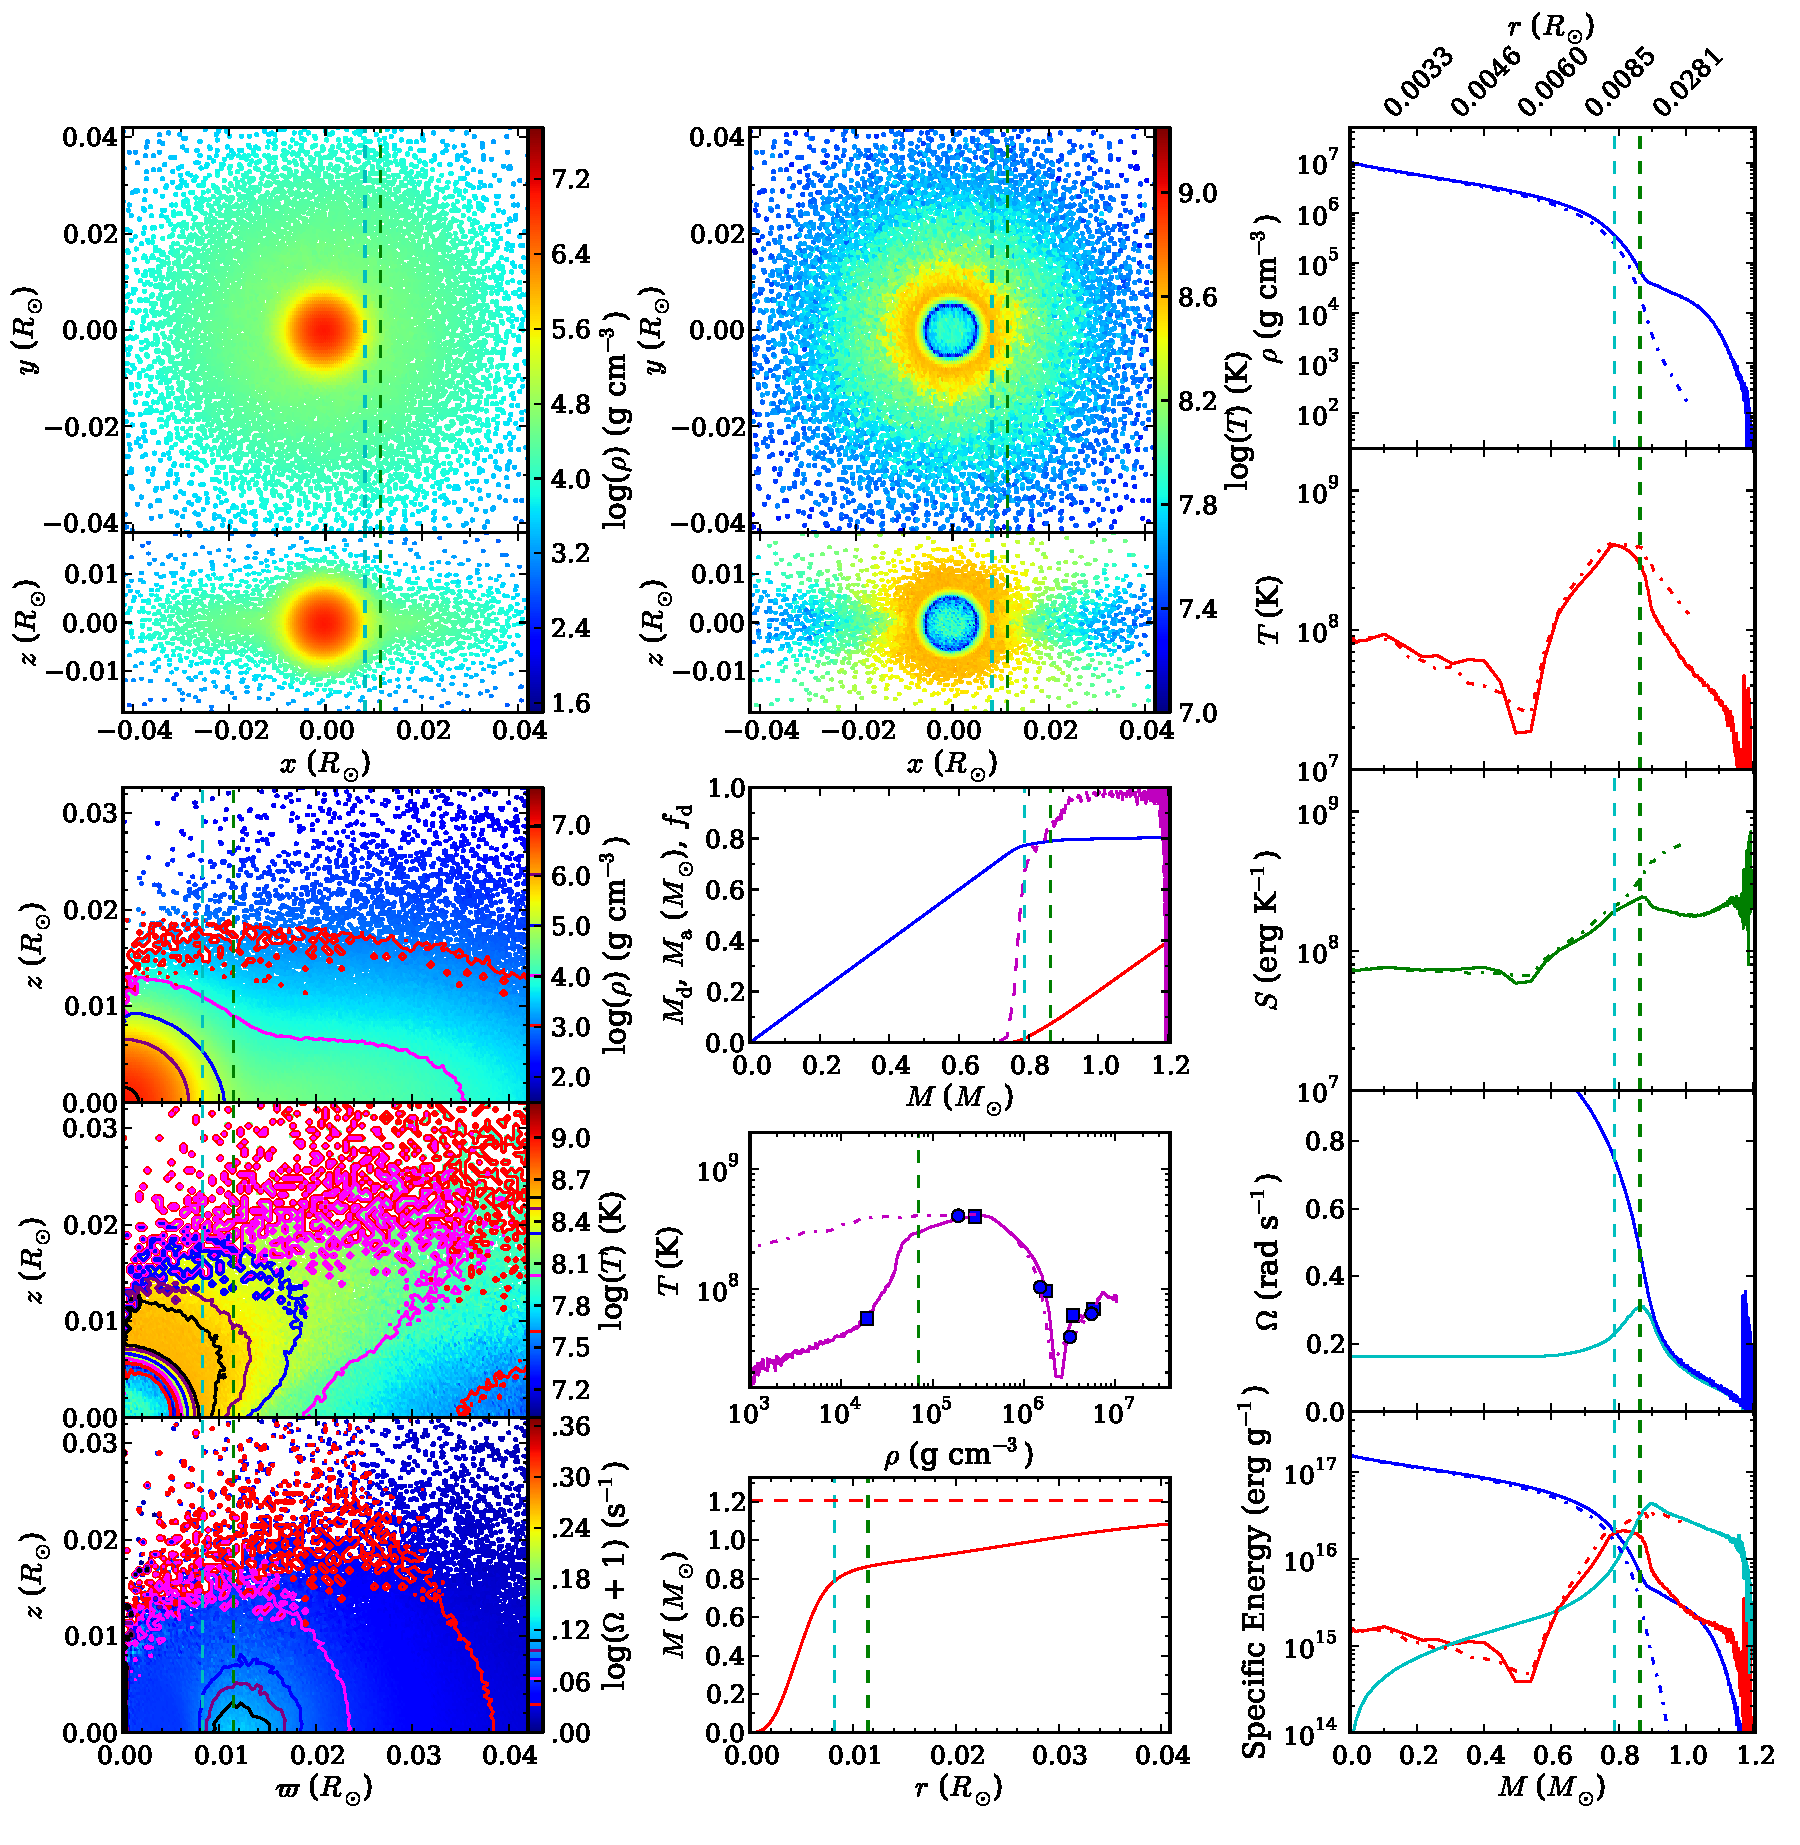
\includegraphics[width=1.0\columnwidth]{chapter2_zhu+13/figures/pt4pt8.pdf}
\caption{Structure of a 0.4 - 0.8 {\Msun} merger remnant, representing the general outcome of a merger of white dwarfs with dissimilar mass.  Upper left and middle -- binned maps of density $\rho$ and temperature $T$ along slices in the $xy$ and $xz$-planes.  Lower left -- binned maps and contours of density, temperature, and angular frequency $\Omega$ in the $(\varpi,z)$ plane, averaged over cylindrical coordinate $\phi$ and over $\pm z$ (with 1 added to $\Omega$ to avoid problems with the logarithmic intensity scale).  Middle -- enclosed masses of donor and accretor material {\Md} and {\Ma} (solid red and blue, resp.), and fraction of donor material \fdon\ at a particular mass shell (dashed magenta).  Middle, one but lowest -- temperature-density profile with enclosed masses in 0.2\,\Msun\ increments indicated, both along the equatorial plane (solid curve, squares) and along the rotational axis (dot-dashed curve, circles).  Middle, bottom -- enclosed mass as a function of $r$, with the total mass indicated by the horizontal dashed red line.  Right-hand column, top to bottom - density, temperature, entropy, angular (cyan) and Keplerian (blue) frequency, and degeneracy (blue), thermal (red) and rotational (cyan) specific energies as a function of enclosed mass $M$, both along the equatorial plane and along the rotational axis (solid and dot-dashed curves, respectively).  In all graphs, the start of the disk (where the centrifugal acceleration equals half the gravitational one) and the equatorial radius (or mass enclosed within) of maximum temperature are marked by vertical green and blue dashed lines, respectively. [{\em See the electronic edition of \cite{zhu+13} for the other remnants}.]}
\label{fig:c2_mergersampling1}
\end{figure}

\begin{figure}
\centering
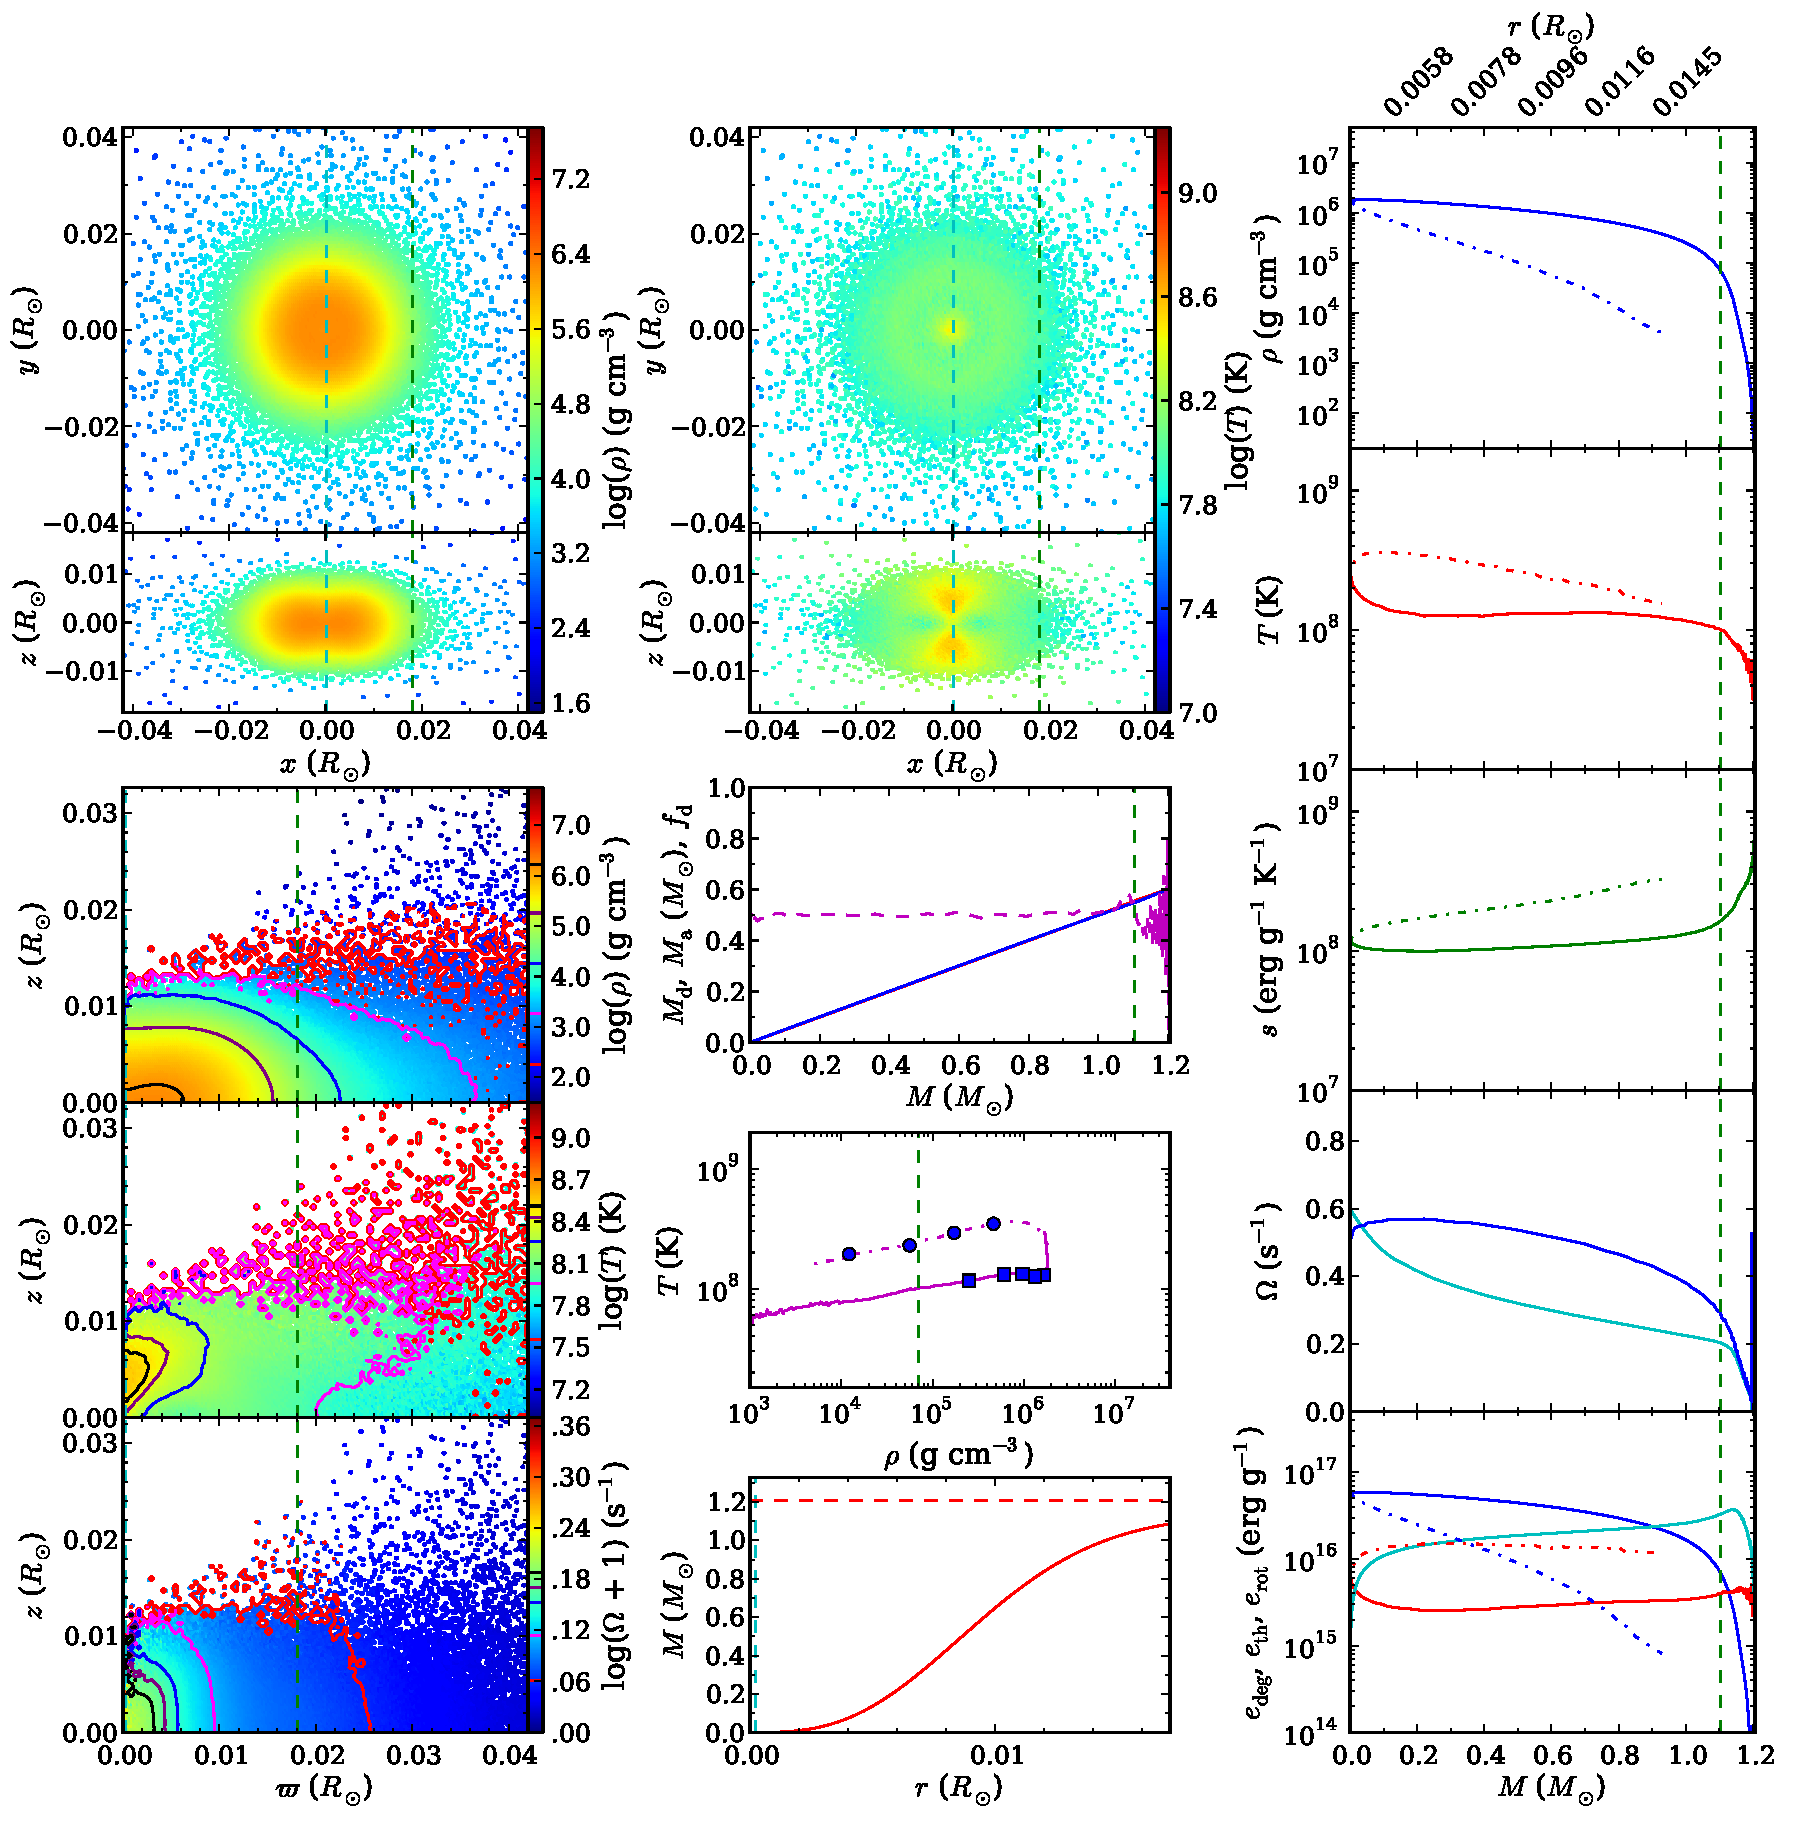
\includegraphics[width=1.0\columnwidth]{chapter2_zhu+13/figures/pt6pt6.pdf}
\caption{As Fig. Set~\ref{fig:c2_mergersampling1}, but for a 0.6 - 0.6 \Msun\ merger remnant, representing the general outcome of a similar-mass merger.}
\label{fig:c2_mergersampling2}
\end{figure}

As found for previous simulations, qualitatively the most important factor controlling the merger outcome is whether the WD masses are ``dissimilar'' or `` similar''.  In the former case, where the donor is significantly less massive than the accretor, only the donor overflows its Roche lobe,\footnote{The lower mass WD is larger and thus always fills its (smaller) Roche lobe first.} is disrupted, and accretes onto the accretor.  The accreted material is heated on impact, lifting degeneracy.  Hence, the merger remnant consists of a partly non-degenerate hot envelope and small, thick sub-Keplerian disk, both surrounding a cold core containing the largely unaffected accretor.

In the latter case of a similar-mass merger, there is a large degree of mixing between the two stars.  For exactly equal masses, both stars are disrupted simultaneously, and their accretion streams impact each other near the system's barycenter.  Material from the centers of both stars initially forms a thick, cold, dense torus orbiting the barycenter; this torus slowly shrinks due to viscous drag, pushing the accretion stream material above and below the equatorial plane.  When the stars have slightly different mass, the lower-mass one disrupts first, forming an accretion stream (or series of streams) that mixes with accretor material down to the center of the accretor (regardless of whether or not the other also disrupts).

We show the differences between similar and dissimilar-mass merger remnants using two representative examples in Figs.~\ref{fig:c2_mergersampling1} and~\ref{fig:c2_mergersampling2}: a 0.4 - 0.8 {\Msun} highly dissimilar and a 0.6 - 0.6 {\Msun} equal-mass merger, respectively.  One sees that the remnant morphologies are very different, consistent with previous work.  The 0.4 - 0.8 {\Msun} merger features a cold, nearly non-rotating and thus spherically symmetric remnant core, surrounded by a hot envelope with roughly equal degeneracy and thermal support, which itself is surrounded on the equatorial plane by a rotationally supported non-degenerate thick disk that holds most of the angular momentum.  The accretor forms the core, largely undisturbed by the merger, while the envelope and disk are composed almost entirely out of donor material.  The hottest points are on the interface between the core and the envelope.\footnote{The higher temperatures near the core are spurious; see Sec.~\ref{ssec:c2_spheat}}  The 0.6 - 0.6 {\Msun} remnant, on the other hand, has a massive, hot, partly rotationally supported and thus ellipsoidal core, and a very small but thick disk, both of which consist of material from both stars.  No distinct envelope is formed.  The hottest points are within the remnant core, just above and below the equatorial plane, arising from accretion stream material pushed out by the shrinking dense torus.

%MHvK: I think the mixing is already implicit in the above, and is better described as part of the discussion of nearly equal vs unequal below
%Mixing is another difference between these classes of mergers.  We show  the cumulative mass of the donor and accretor in the second column, third row plot in Figs. \ref{fig:c2_mergersampling1} and \ref{fig:c2_mergersampling2}.  For the unequal mass case, the cumulative mass curve of the donor only becomes non-zero when the cumulative mass of the accretor asymptotes, indicating negligible mixing, while for the 0.6 - 0.6 {\Msun} merger the two curves lie nearly on top of one another, indicating uniform mixing. 

%Comparison with other equal and unequal mass mergers show that the qualitative features of the 0.4 - 0.8 {\Msun} remnant extend to all unequal mass mergers, while those of the 0.6 - 0.6 {\Msun} remnant all equal mass mergers.

%MHvK: this belongs in caption
%Different colors represent different donor masses: red = 0.4 {\Msun}, orange = 0.5 {\Msun}, lime = 0.55 {\Msun}, green = 0.575 {\Msun}, cyan = 0.6 {\Msun}, sky blue = 0.625 {\Msun}, blue = 0.64 {\Msun}, dark blue = 0.65 {\Msun}, magenta = 0.7 {\Msun}, purple = 0.8 {\Msun}, brown = 0.9 {\Msun} and black = 1.0 {\Msun}. 

A good way to visualize how mergers transition between dissimilar and similar-mass is to look at changes in the remnant properties with varying donor mass.  In Fig. \ref{fig:c2_constacc}, we show curves for accretors of 0.65 (left) and 1.0\,\Msun (right).  One sees that remnants of highly dissimilar-mass mergers, with mass ratio $\qm\equiv M_\mrm{d}/M_\mrm{a} \lesssim0.5$, have properties resembling the 0.4 - 0.8 {\Msun} merger: their donor and accretor barely mixed, their temperature curves have off-center hot plateaus, and their angular velocity profiles feature an off-center bump.  The equal-mass, $\qm=1$ cases resemble the 0.6 - 0.6 {\Msun} remnant: they have flat temperature profiles and centrally peaked angular velocity profiles.  Intermediate cases have intermediate profiles, with the bumps in the temperature and angular velocity profiles widening with increasing {\qm}.  The 0.4 - 0.8 {\Msun} and 0.6 - 0.6 {\Msun} remnants therefore lie at the extremes of what merger remnants look like.

%and all merger remnants studied fall on the continuum between these two extremes.  {\bf move this last sentence later}Note that the 1.0 {\Msun} accretor runs show more spurious heating than the 0.65 {\Msun} accretor runs.

The similarity between some of the curves for the 0.65 and 1.0\,\Msun\ accretors in Fig. \ref{fig:c2_constacc} suggests a homology.  The similarity is closest for mergers with the same mass difference $\Delta M$, as can be seen in Fig. \ref{fig:c2_deltamcomp}.
%As the homology is not exact, we have defined this as a ``quasi-homology.'' 
For equal-mass mergers, all profiles are similar, simply scaled by a factor that depends on the total mass (except the 1.0 - 1.0 {\Msun} merger; see below).  As $\Delta M$ increases, the profiles are slightly less similar: with increasing total binary mass, the degree of mixing decreases, and the temperature and angular velocity maxima drift to slightly lower fractional enclosed mass.  Nevertheless, the profiles still resemble one another far more closely than they resemble curves with other $\Delta M$.  The same holds for profiles along the rotational axis.

It may seem surprising that the controlling parameter between these approximate homologies is the mass difference $\Delta M$ rather than the mass ratio {\qm}.  Empirically, however, the case is clear: e.g., the 0.4 - 0.5 (second column, yellow) and 0.8 - 1.0 {\Msun} (third column, black) mergers have the same {\qm}, but different $\Delta M$, and their structures clearly differ from one another.  The same is true for the 0.4 - 0.6 (third column, cyan) and 0.6 - 0.9 (fourth column, brown) {\Msun} mergers.  As we discuss below, the similarity of mergers of similar $\Delta M$ likely reflects the close relation between the ratio of central densities and mass difference.  

Before discussing the homologies and trends further, we should note the one dramatic exception.  The 1.0 - 1.0 {\Msun} simulation differs fundamentally from its fellow $\Delta M\,=\,0$ mergers.  During the evolution of this system, unlike for all other equal-mass mergers, one WD was fully disrupted before the other, and as a result material from one star (arbitrarily designated the ``donor'' before the start of simulation, hence the ``inverted'' mixing profile in Figs.~\ref{fig:c2_constacc} and~\ref{fig:c2_deltamcomp}) preferentially resides near the center of the remnant.  This system also often appears as an outlier in Sec.~\ref{ssec:c2_mergertrends} below.  The 0.9 - 0.9 {\Msun} merger also did not have equal mixing between the two stars, though the difference is much smaller.  \cite{rask+12} noticed the same effect in their simulations, and concluded it reflected the fact that more massive WDs are much more concentrated and therefore harder to disrupt.  This seems a likely explanation.

%Hindsight (after submission?), extra runs with 0.05 difference?

\begin{figure}
\centering
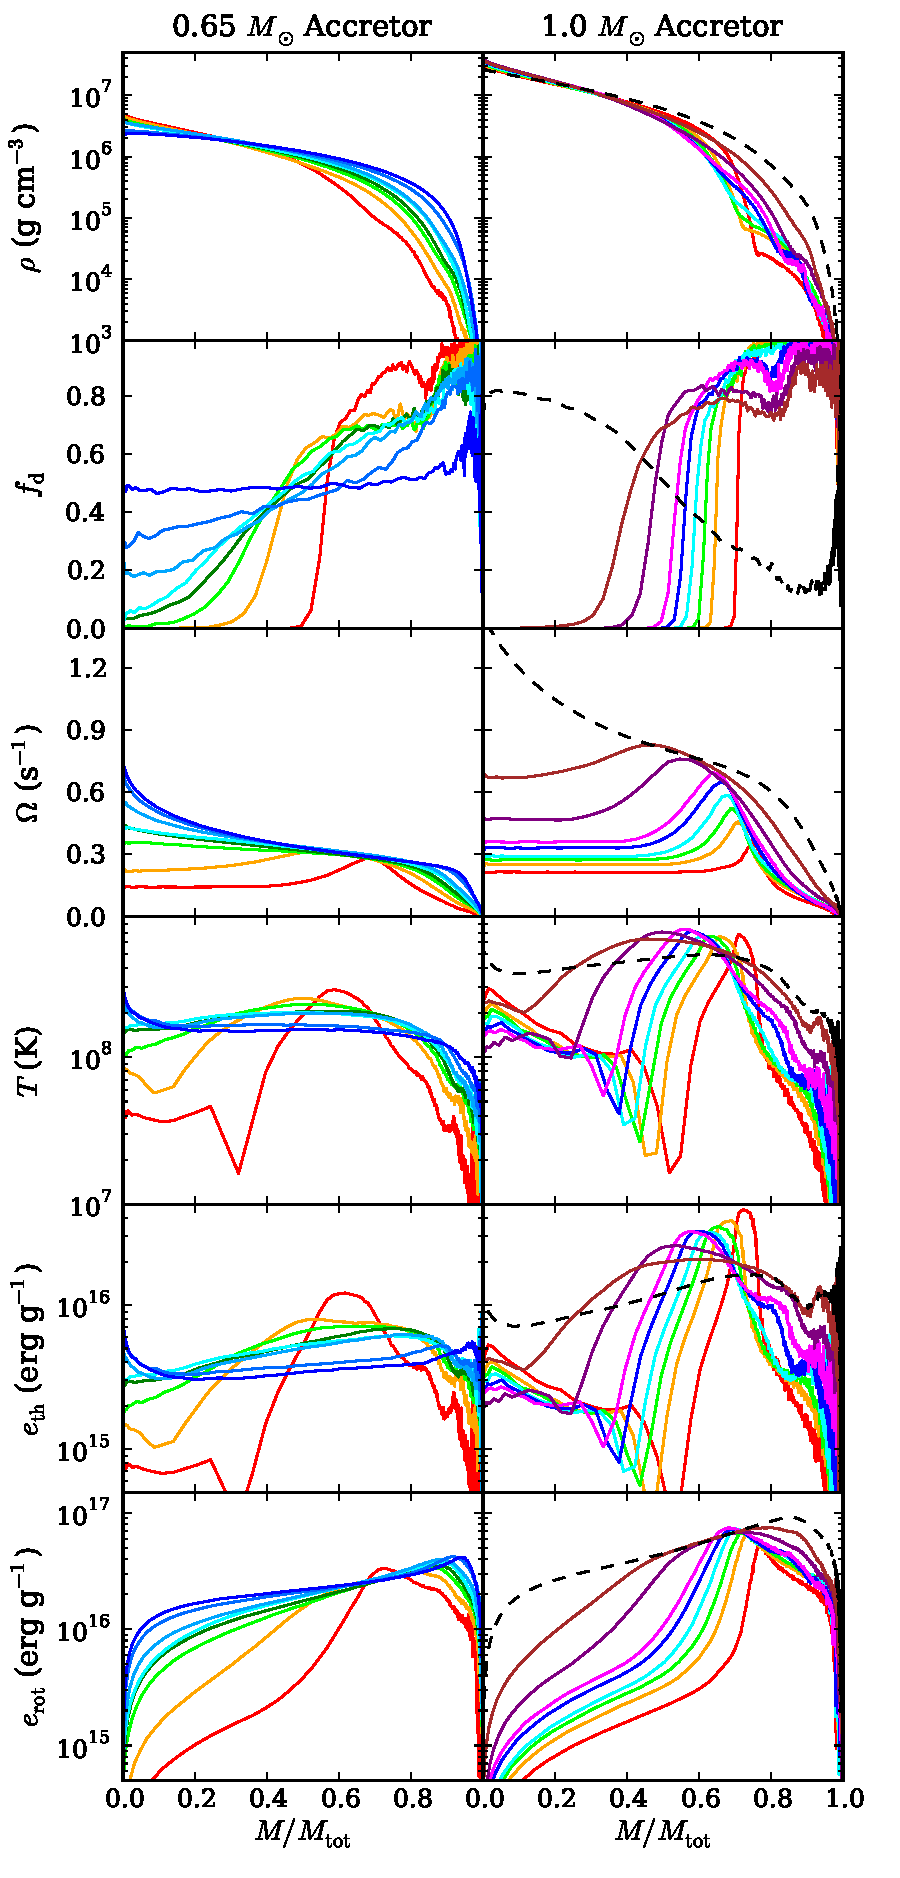
\includegraphics[angle=0,width=0.6\columnwidth]{chapter2_zhu+13/figures/constaccretorcomp.pdf}
\caption{Properties of mergers with 0.65\,\Msun\ (left) and 1.0\,\Msun\ (right) accretors, for donor masses of 0.4 (red), 0.5 (orange), 0.55 (lime), 0.575 (green), 0.6 (cyan), 0.625 (light blue), 0.64 (blue), 0.65 (dark blue), 0.7 (magenta), 0.8 (purple), 0.9 (brown), and 1.0\,\Msun\ (black).  Shown are, from top to bottom, density $\rho$, fraction of donor material \fdon, angular frequency $\Omega$, temperature $T$, specific thermal energy $E_{\rm th}$, and specific rotational energy $E_{\rm rot}$, all as a function of fractional enclosed mass $M/M_{\rm tot}$.  All properties are determined along the equatorial plane, except for \fdon\ which is defined spherically.  The 1.0 - 1.0 {\Msun} merger (dashed black line) is an outlier; see text.}
\label{fig:c2_constacc}
\end{figure}

\begin{figure}
\centering
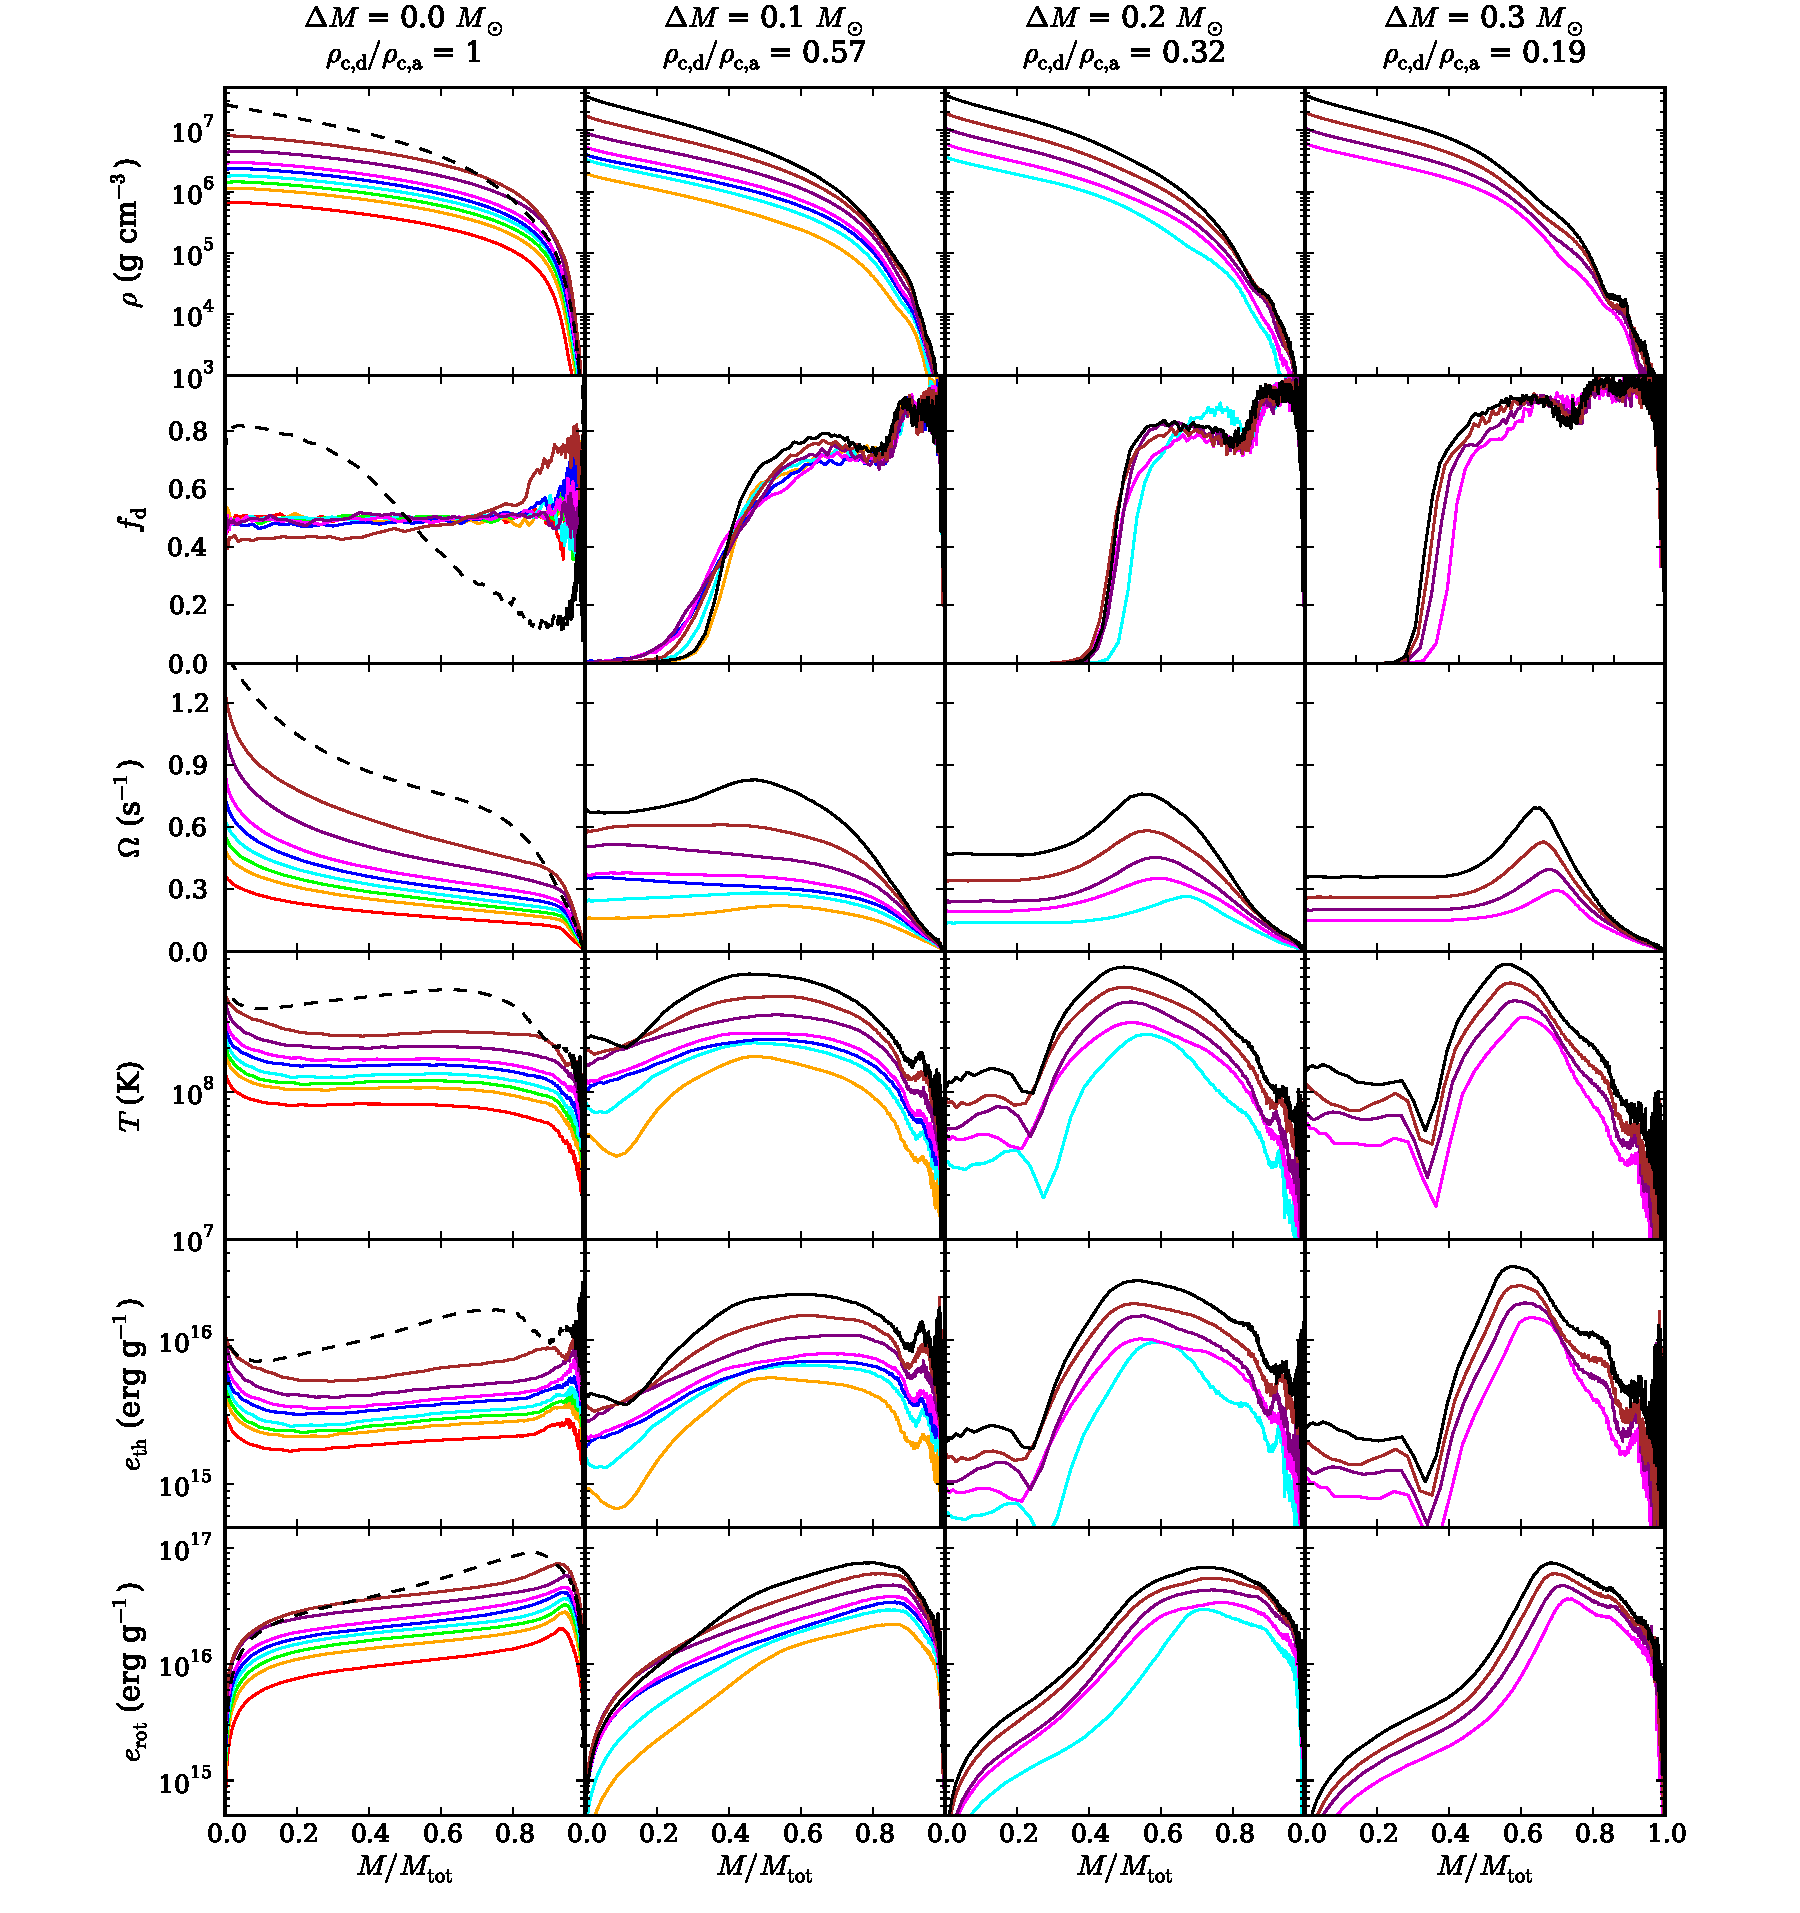
\includegraphics[angle=0,width=1.0\columnwidth]{chapter2_zhu+13/figures/deltamcomp.pdf}
\caption{Dependence of the properties of mergers on mass difference, with, from left to right, $\Delta M \equiv $ {\Ma} - {\Md} = 0.0, 0.1, 0.2, and $0.3\,\Msun$ mergers.  Properties shown, coloring, and line styles are as in Fig.~\ref{fig:c2_constacc}, except color represents accretor mass.}
\label{fig:c2_deltamcomp}
\end{figure}

\subsection{Merger Trends}
\label{ssec:c2_mergertrends}

A major goal of our work is to establish how various global properties of the merger remnant, such as remnant core and disk mass, maximum temperature, and maximum angular velocity, vary as a function of accretor and donor mass.  By quantifying these trends, we hope to help develop a parametrized model of merger remnants.  Before discussing trends, however, we stress that they are necessarily \textit{approximate} - second order effects, numerical noise and our choice of stopping time all affect the remnant properties.  Moreover, while integrated values like total thermal energy do not fluctuate from timestep to timestep, values at specific points in the remnant do (as noted the following sections).  For instance, the mass enclosed within the radius of peak equatorial temperature becomes ill-defined for similar-mass mergers because these have rather flat temperature profiles (Fig.~\ref{fig:c2_constacc}).  To partly mitigate these fluctuations, the values presented below were determined by averaging frames from the simulation over an eight second span, centered on the time corresponding to six orbits of the initial binary.

As might be expected from the approximate homologies described above, we found that many properties scaled well with $\Delta M$.  Of course, a scaling with a dimensional mass difference makes little sense; we believe its success reflects the fact that over the range of 0.4 -- 1.0\,{\Msun}, the central density {\rhoc} depends approximately exponentially on mass, with $\rho_{c} \simeq 3.3\times10^7{\rm\,g\,cm^{-3}} \exp[5.64(M/\Msun-1)]$ (see Fig.~\ref{fig:c2_mrho}).  Hence, a given mass difference $\Delta M$ corresponds to a given ratio of central densities, \rhocrat.  As argued in Sec.~\ref{sssec:c2_masstrends}, \rhocrat\ has a straightforward interpretation: it characterizes the degree of mixing between the donor and accretor.  We therefore discuss trends as a function of $\qrho\equiv\rhocrat$ from hereon.  Where necessary, we refer to the mass ratio as \qm.

%MHvK: superfluous after the above.
%We chose to plot every trend presented below as a function of {\qrho}.  This was not only because doing so makes comparisons between different trends easier, but also because due to the quasi-homology {\qrho}, i.e., $\Delta M$, parametrizes the majority of the trends presented.

\begin{figure}
\centering
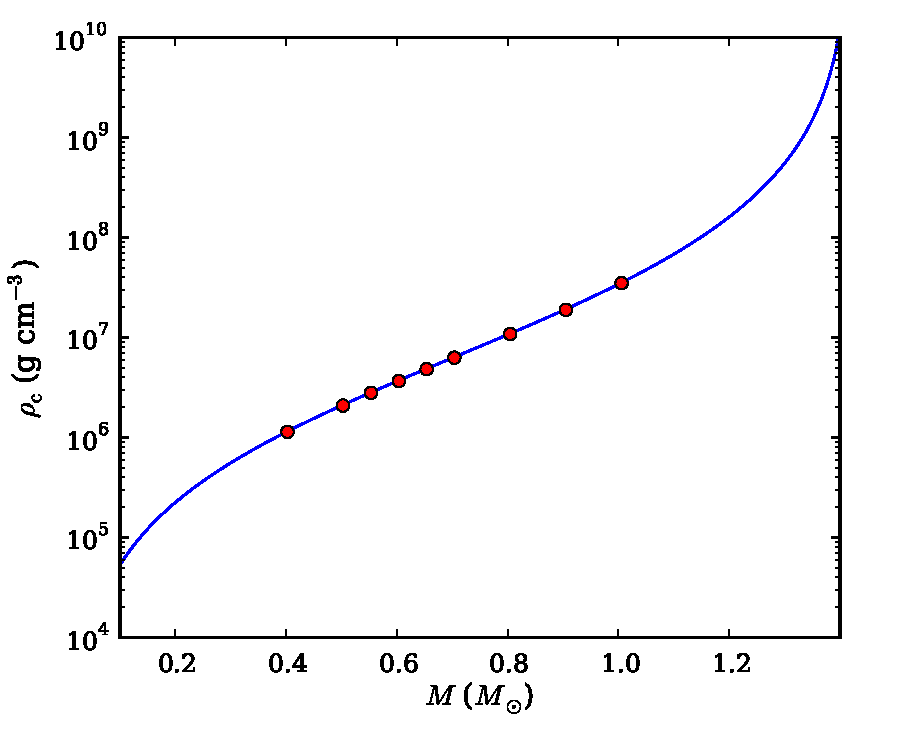
\includegraphics[angle=0,width=0.6\columnwidth]{chapter2_zhu+13/figures/Mrhorelation.pdf}
\caption{Relation between central density \rhoc\ and mass $M$ for carbon-oxygen white dwarfs, showing both the results of relaxing white dwarf models in Gasoline (red points), and integrating hydrostatic equilibrium directly for spherically symmetric, non-rotating CO WDs with $T=5\times 10^6\,$K (blue line).  For the mass range considered, the central density depends roughly exponentially on mass.}
\label{fig:c2_mrho}
\end{figure}

\subsubsection{What Constitutes Similar-Mass?}
\label{sssec:c2_whatisequalmass}

%\citeal{vkercj10}'s SN Ia channel is optimal when the hottest temperature in the merger remnant is at its center\qc{, i.e., equal-mass mergers}. 

As {\qrho} increases from a small value toward unity, the merger remnant's morphology shifts from resembling Fig.~\ref{fig:c2_mergersampling1} (dissimilar-mass) to resembling Fig.~\ref{fig:c2_mergersampling2} (equal-mass).  From Fig.~\ref{fig:c2_constacc}, ones sees that there is no particular {\qrho} at which one transitions from ``dissimilar'' to ``similar.''  Nevertheless, we can determine a rough critical value of~{\qrho} that separates mergers in which the core is largely unaffected from those in which it is changed significantly, a separation that likely affects the outcome of post-merger evolution.

%{\bf MHvK: note that I introduced new nomenclature, in the ratio of donor to accretor material.}
To determine the critical value, we show in Fig.~\ref{fig:c2_eqmass} the ratio of central to maximum temperature, $T_\mrm{c}/T_{\rm max}$, central to maximum angular velocity, $\Omega_\mrm{c}/\Omega_{\rm max}$, and the fraction of donor to accretor material within the central core, \fratio, where we define the central core as a sphere with radius \hz.  All three properties are measures of the extent to which the core has been affected: mixed regions tend to be hotter and more spun up, and contain material from both stars.

From Fig.~\ref{fig:c2_eqmass}, one sees that $\Omega_\mrm{c}/\Omega_\mathrm{max}$ approaches unity at $q_\rho\simeq0.6$; at higher values, the angular velocity profile has a plateau or central peak rather than an off-center bump.  Also at $q_\rho\simeq0.6$, \fratio\ starts to deviate from zero, i.e., donor material begins to penetrate the central core.  The temperature points show the transition is not abrupt: $T_\mathrm{c}/T_\mathrm{max}$ starts to deviate from its downward trend (which reflects spurious heating in the most dissimilar-mass mergers; Sec.~\ref{ssec:c2_spheat}) around $q_\rho\simeq0.3$ and continues to increase until $q_\rho=1.0$; at $q_\rho\simeq0.6$, $T_\mathrm{c}/T_\mathrm{max}\simeq0.5$.  Overall, this suggests that while the dependence is gradual, the morphology changes most around $\qrho\simeq0.6$.  This conclusion is confirmed by looking at the two-dimensional remnant temperature structures (Figs.~\ref{fig:c2_mergersampling1} and~\ref{fig:c2_mergersampling2}).  At $q_\rho\ll0.6$, the remnant core has a large, spherically symmetric cold region, the nearly unperturbed accretor.  This cold region shrinks with increasing \qrho, and at $q_\rho\simeq0.6$, spherical symmetry is broken.  For still larger \qrho, the cold region becomes a flat slice sandwiched between hotspots off the equatorial plane.

Given the above, we define ``similar-mass'' mergers as those with donor to accretor central density ratio $q_\rho>0.6$, and ``dissimilar-mass'' mergers as those with $q_\rho<0.6$.  This critical density ratio corresponds to a mass difference $\Delta M\simeq0.1\,\Msun$.

\begin{figure}
\centering
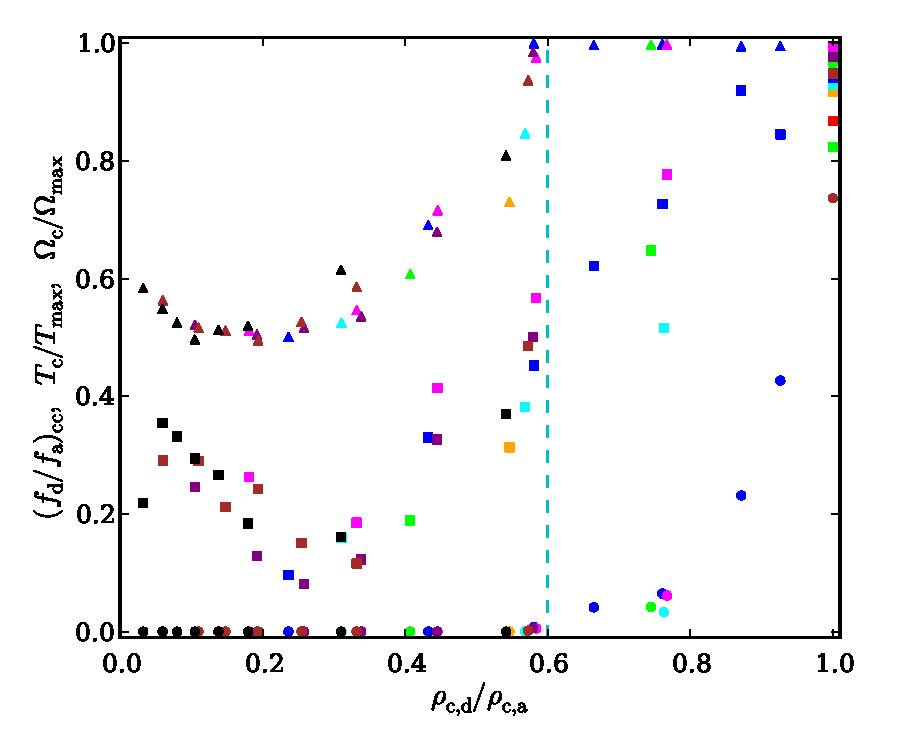
\includegraphics[width=0.6\columnwidth]{chapter2_zhu+13/figures/Eqmass.pdf}
\caption{Dependence of merger core properties on the ratio of the donor and accretor central densities, \rhocrat.  Shown are the ratio of central to maximum temperature $T_\mathrm{c}/T_\mathrm{max}$ (squares), central to maximum angular velocity $\Omega_\mathrm{c}/\Omega_\mathrm{max}$ (triangles), and central core donor to accretor mass fraction \fratio\ (circles), with colors representing different accretor masses, encoded as in Fig.~\ref{fig:c2_constacc}.  The vertical line marks $\qrho\equiv\rhocrat=0.6$, where $\Omega_\mathrm{c}/\Omega_\mathrm{max}$ reaches unity, \fratio\ becomes non-zero, and $T_\mathrm{c}/T_\mathrm{max}\simeq0.5$.  We suggest it separates ``dissimilar'' from ''similar'' mass mergers.}
\label{fig:c2_eqmass}
\end{figure}

\subsubsection{Structural Trends}
\label{sssec:c2_structuraltrends}

Here and in the following subsections of \ref{ssec:c2_mergertrends}, we describe various trends of remnant properties in detail, hoping to help attempts to interpolate between different simulations and motivate analytical and semi-analytical depictions of the merger.  Readers not requiring this level of detail may wish to skip to Sec. \ref{ssec:c2_qualitative}.  We begin our discussion of trends with size and density parameters.

\paragraph{The rotational axis central scaleheight.} We define the rotational axis central scaleheight \hz\ as the characteristic width $\sigma$ of a Gaussian fit to the density distribution along the $z$ axis at $\varpi = 0$.  \hz\ is a measure of the vertical extent of the remnant.  We find that the ratio $\hz/h_{\rm a}$, where $h_\mathrm{a}$ is the central scaleheight of the accretor, is reasonably well-approximated by,
\eqbegin
\frac{h_\mrm{z}}{h_\mathrm{a}} = 1.03 - 0.17\qrho^{1/2}
\qquad(\pm0.02),
\eqend
where the uncertainty listed in parentheses represents the root-mean-square (RMS) of the residuals around the approximation (see Fig.~\ref{fig:c2_structuretrends}a).  For highly dissimilar-mass mergers, \hz\ approximately equals the scaleheight of the accretor, while for similar-mass mergers, \hz\ is lower due to rotational support.

The vertical scaleheight increases with increasing $\varpi$: the scaleheight at the location of maximum temperature, $h(T_{\rm max})$, ranges from \hz\ to 1.21\hz, and the scaleheight at maximum angular velocity $h(\Omega_{\rm max})$ ranges from \hz\ to 1.88\hz.  The prefactor for both heights increases with increasing accretor mass {\Ma} and decreasing \qrho. 

\paragraph{The equatorial plane central scaleheight.}  Similar to \hz\, we define \hxy\ -- the characteristic width of a Gaussian fit to the density distribution along the equatorial plane -- as a measure of the equatorial extent of the remnant.  The ratio $\hxy/h_{\rm a}$ can be parametrized by
\eqbegin
\frac{\hxy}{h_{\rm a}} = 0.96 + 0.89q_\rho^2
\qquad(\pm0.08),
\eqend
where we excluded the 1.0 - 1.0 {\Msun} merger remnant for our fit (see Fig.~\ref{fig:c2_structuretrends}a).  The dependence on increasing \qrho\ reflects the increased rotational support of the remnant core.

\paragraph{The central density of the remnant.}  The central density, \rhoc, is always within a factor two of the central density of the accretor, \rhoca.  In Fig.~\ref{fig:c2_structuretrends}b, one sees that for given accretor mass, \rhocrhoct\ increases with increasing \qrho\ for highly dissimilar-mass mergers due to increasing compression of the remnant core, but begins to decrease because of increasing rotational support around $\qrho\simeq0.3$.  We could not find a simple parametrization for these curves.  Note that for some systems, as we continue running our simulations \rhocrhoct\ continues to increase.  As discussed in Sec.~\ref{ssec:c2_mergercomplete}, this is probably because artificial viscosity forces the merger remnant to undergo accelerated viscous evolution.

%\textbf{Actually I did find a term that can linearize central density: $M_\mathrm{a,enc}(\rho_\mathrm{d,c})/(M_\mathrm{a} - M_\mathrm{d})$ (i.e. the mass of material in the accretor with a higher density than the central density of the donor, scaled by $\Delta M$.  I don't have a clue as to what it means, though.}

%\end{itemize}

\begin{figure}
\centering
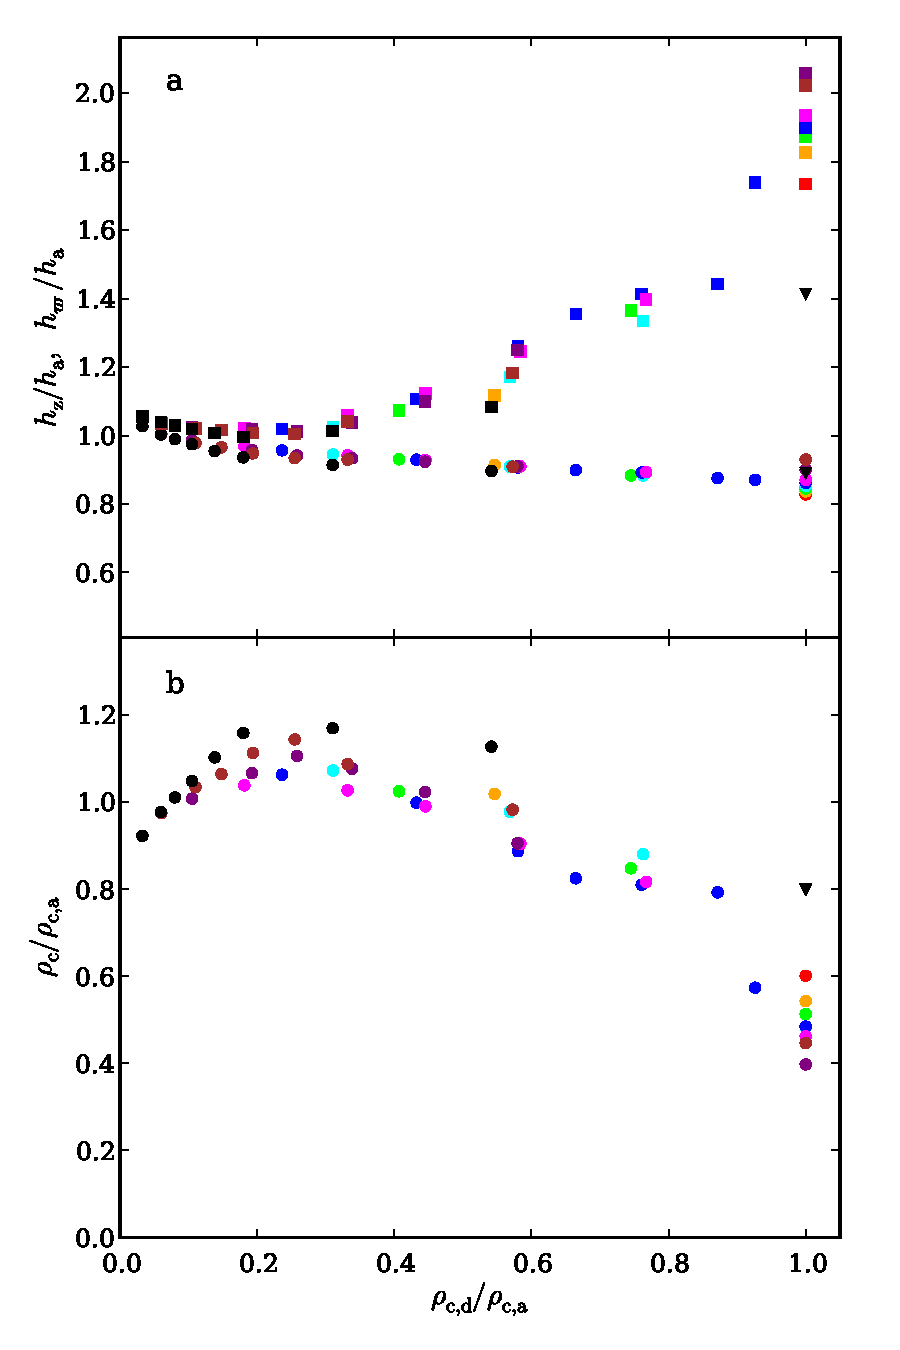
\includegraphics[angle=0,width=0.6\columnwidth]{chapter2_zhu+13/figures/StructureTrendsq.pdf}
\caption{Structural properties of mergers.  (a) Central scaleheights along the rotational axis (circles) and along the equatorial plane (squares) scaled to the scaleheight of the accretor, {\hz}/$h_\mathrm{a}$ and $\hxy$/$h_\mathrm{a}$.  (b) Central density of the merger remnant scaled to the central density of the accretor, {\rhocrhoct}.  Colors represent different accretor masses, encoded as in Fig.~\ref{fig:c2_constacc}.  Triangles represent the outlying 1.0 - 1.0\,\Msun\ merger.}
\label{fig:c2_structuretrends}
\end{figure}

\subsubsection{Mass Distributions}
\label{sssec:c2_masstrends}

The merger mixes material between the donor and accretor.  Here, we describe how this changes as a function of \qrho, as well as how the material is distributed between the pressure-supported core and envelope and the rotationally supported disk.

\paragraph{The masses of the core-envelope and disk.}  We formally define the core-envelope as the part of the remnant inside the inner disk radius $\varpi_\mrm{disk}$, i.e., that is supported primarily by pressure (degeneracy for the core, thermal for the envelope) and not rotation.  Since in every merger very little mass is ejected, a trend for either the core-envelope or the disk mass (\Mrem\ and \Mdisk, resp.) suffices to determine both.  The ratio of \Mrem\ to the accretor mass \Ma\ is well described by,
\eqbegin
\frac{\Mrem}{\Ma} = 1 + 0.81\qrho
\qquad(\pm0.03),
\eqend
if the 1.0 - 1.0 {\Msun} merger is neglected, and the fit's $y$-intercept is forced to unity.  See Fig.~\ref{fig:c2_restoftrends}a.

%(see the dashed green line in Figs.~\ref{fig:c2_mergersampling1} and~\ref{fig:c2_mergersampling2})

\paragraph{The mass enclosing 50\% of the donor material.}  The further the donor penetrates, the smaller will be the mass enclosing half the donor's material, \MMfifty.  For mergers with $\qrho\lesssim0.8$, $\MMfifty/\Ma\,\simeq\,1.30$, with an RMS residual of 0.03 (Fig.~\ref{fig:c2_restoftrends}c).  We present this trend mostly because we discuss similar thermodynamic and rotational enclosed masses, but it is somewhat difficult to interpret physically, since \MMfifty\ increases with donor mass but decreases with mixing, which also depends on donor mass.  The trend is easier to interpret using enclosed accretor mass rather enclosed total mass, as done below.

\paragraph{The accretor mass enclosing 50\% of the donor material.}  As a different measure of the depth to which the donor penetrates, we consider just the accretor material within the mass enclosing half the donor, $\MMfifty-\frac{1}{2}\Md$.  This should equal the accretor mass if the donor is deposited above the accretor, and half the accretor mass if the two stars are completely mixed.  For $\qrho\lesssim0.8$, it can be approximated by (Fig.~\ref{fig:c2_restoftrends}b),
\eqbegin
\frac{\MMfifty-\frac{1}{2}\Md}{\Ma} = 1 - 0.190\qrho
\qquad(\pm0.009),
\eqend
where we forced the intercept to be unity.  In this regime, roughly half of the donor remains outside of the accretor, though the trend discussed next indicates that the other half which does penetrate the accretor is spread across a much larger region at higher \qrho.  When $q_\rho\gtrsim0.8$, the ratio drops sharply downward, indicative of the more thorough mixing expected for the similar-mass case.  However, the existence and exact location of this drop may be a function of initial conditions (see Sect.~\ref{ssec:c2_varyingazero}).  

\paragraph{The region over which the donor is spread.} As a measure of the thickness of the region affected by the merger, we use the difference of the mass enclosing 75\% of the donor material with that enclosing 25\% of the donor material, i.e., $\MMthick = M_{\rm enc}(\frac{3}{4}\Md) - M_{\rm enc}(\frac{1}{4}\Md)$.  Since 50\% of the donor is within this range, $\MMthick - \frac{1}{2}\Md$ is a measure of the amount of accretor mixed with the donor.  For $q_\rho\lesssim0.8$, the ratio of the latter to the total accretor mass follows,
\eqbegin
\frac{\MMthick-\frac{1}{2}\Md}{\Ma} = 0.30\qrho
\qquad(\pm0.02),
\eqend
while for $q_\rho\gtrsim0.8$ the trend curls upward until it reaches 0.5, the value expected for completely mixed remnants.  See Fig. \ref{fig:c2_restoftrends}d.

Combining the two above trends, we can formulate a qualitative picture of mixing.  For $q_\rho\lesssim0.8$, the donor can be thought of as being deposited onto the accretor and mixing with the accretor's outer layers, while for $q_\rho\gtrsim0.8$, the accretor also disrupts substantially, leading to a regime where both stars mix more uniformly.  The region over which the donor is spread, or thickness of the mixed layer, in both cases depends on {\qrho}, which suggests that the relative densities of the donor and accretor govern mixing, i.e., the donor mixes significantly with all accretor material up to some fraction of the central density of the donor.  Additional evidence of this will be seen in the thermodynamic trends below.  

One might consider an alternate picture in which the donor dredges up a constant fraction of its own mass in accretor material.  If this were the case, we would expect $(\MMthick-\frac{1}{2}\Md)/\Md$ to roughly be constant.  Our results, however, show that for $q_\rho\lesssim0.8$ this quantity is nearly a straight line that is close to zero for small \qrho\ ($(\MMthick-\frac{1}{2}\Md)/\Md = 0.35\qrho\pm0.02$).  This seems more consistent with mixing being determined by density.

%\begin{figure}
%\centering
%\includegraphics[angle=0,width=0.7\columnwidth]{MassTrendsq.pdf}
%\caption{Top: Mass enclosing half of the donor mass scaled to the accretor mass {\MMfifty}/{\Ma}.  Center: width of mixing scaled to the accretor mass ($\Delta M(M_\mathrm{d}) - \frac{1}{2}${\Md})/{\Ma}.  We define $\Delta M(M_\mathrm{d})$ as $M(0.75M_\mathrm{d}) - M(0.25M_\mathrm{d})$.  Right: remnant mass divided by accretor mass{\Mrem}/{\Ma}.  Colors (Fig. \ref{fig:c2_constacc} caption) represent different accretor masses.  Upside-down triangles represent points that are likely outliers.}
%\label{fig:c2_masstrends}
%\end{figure}

\begin{figure*}
\centering
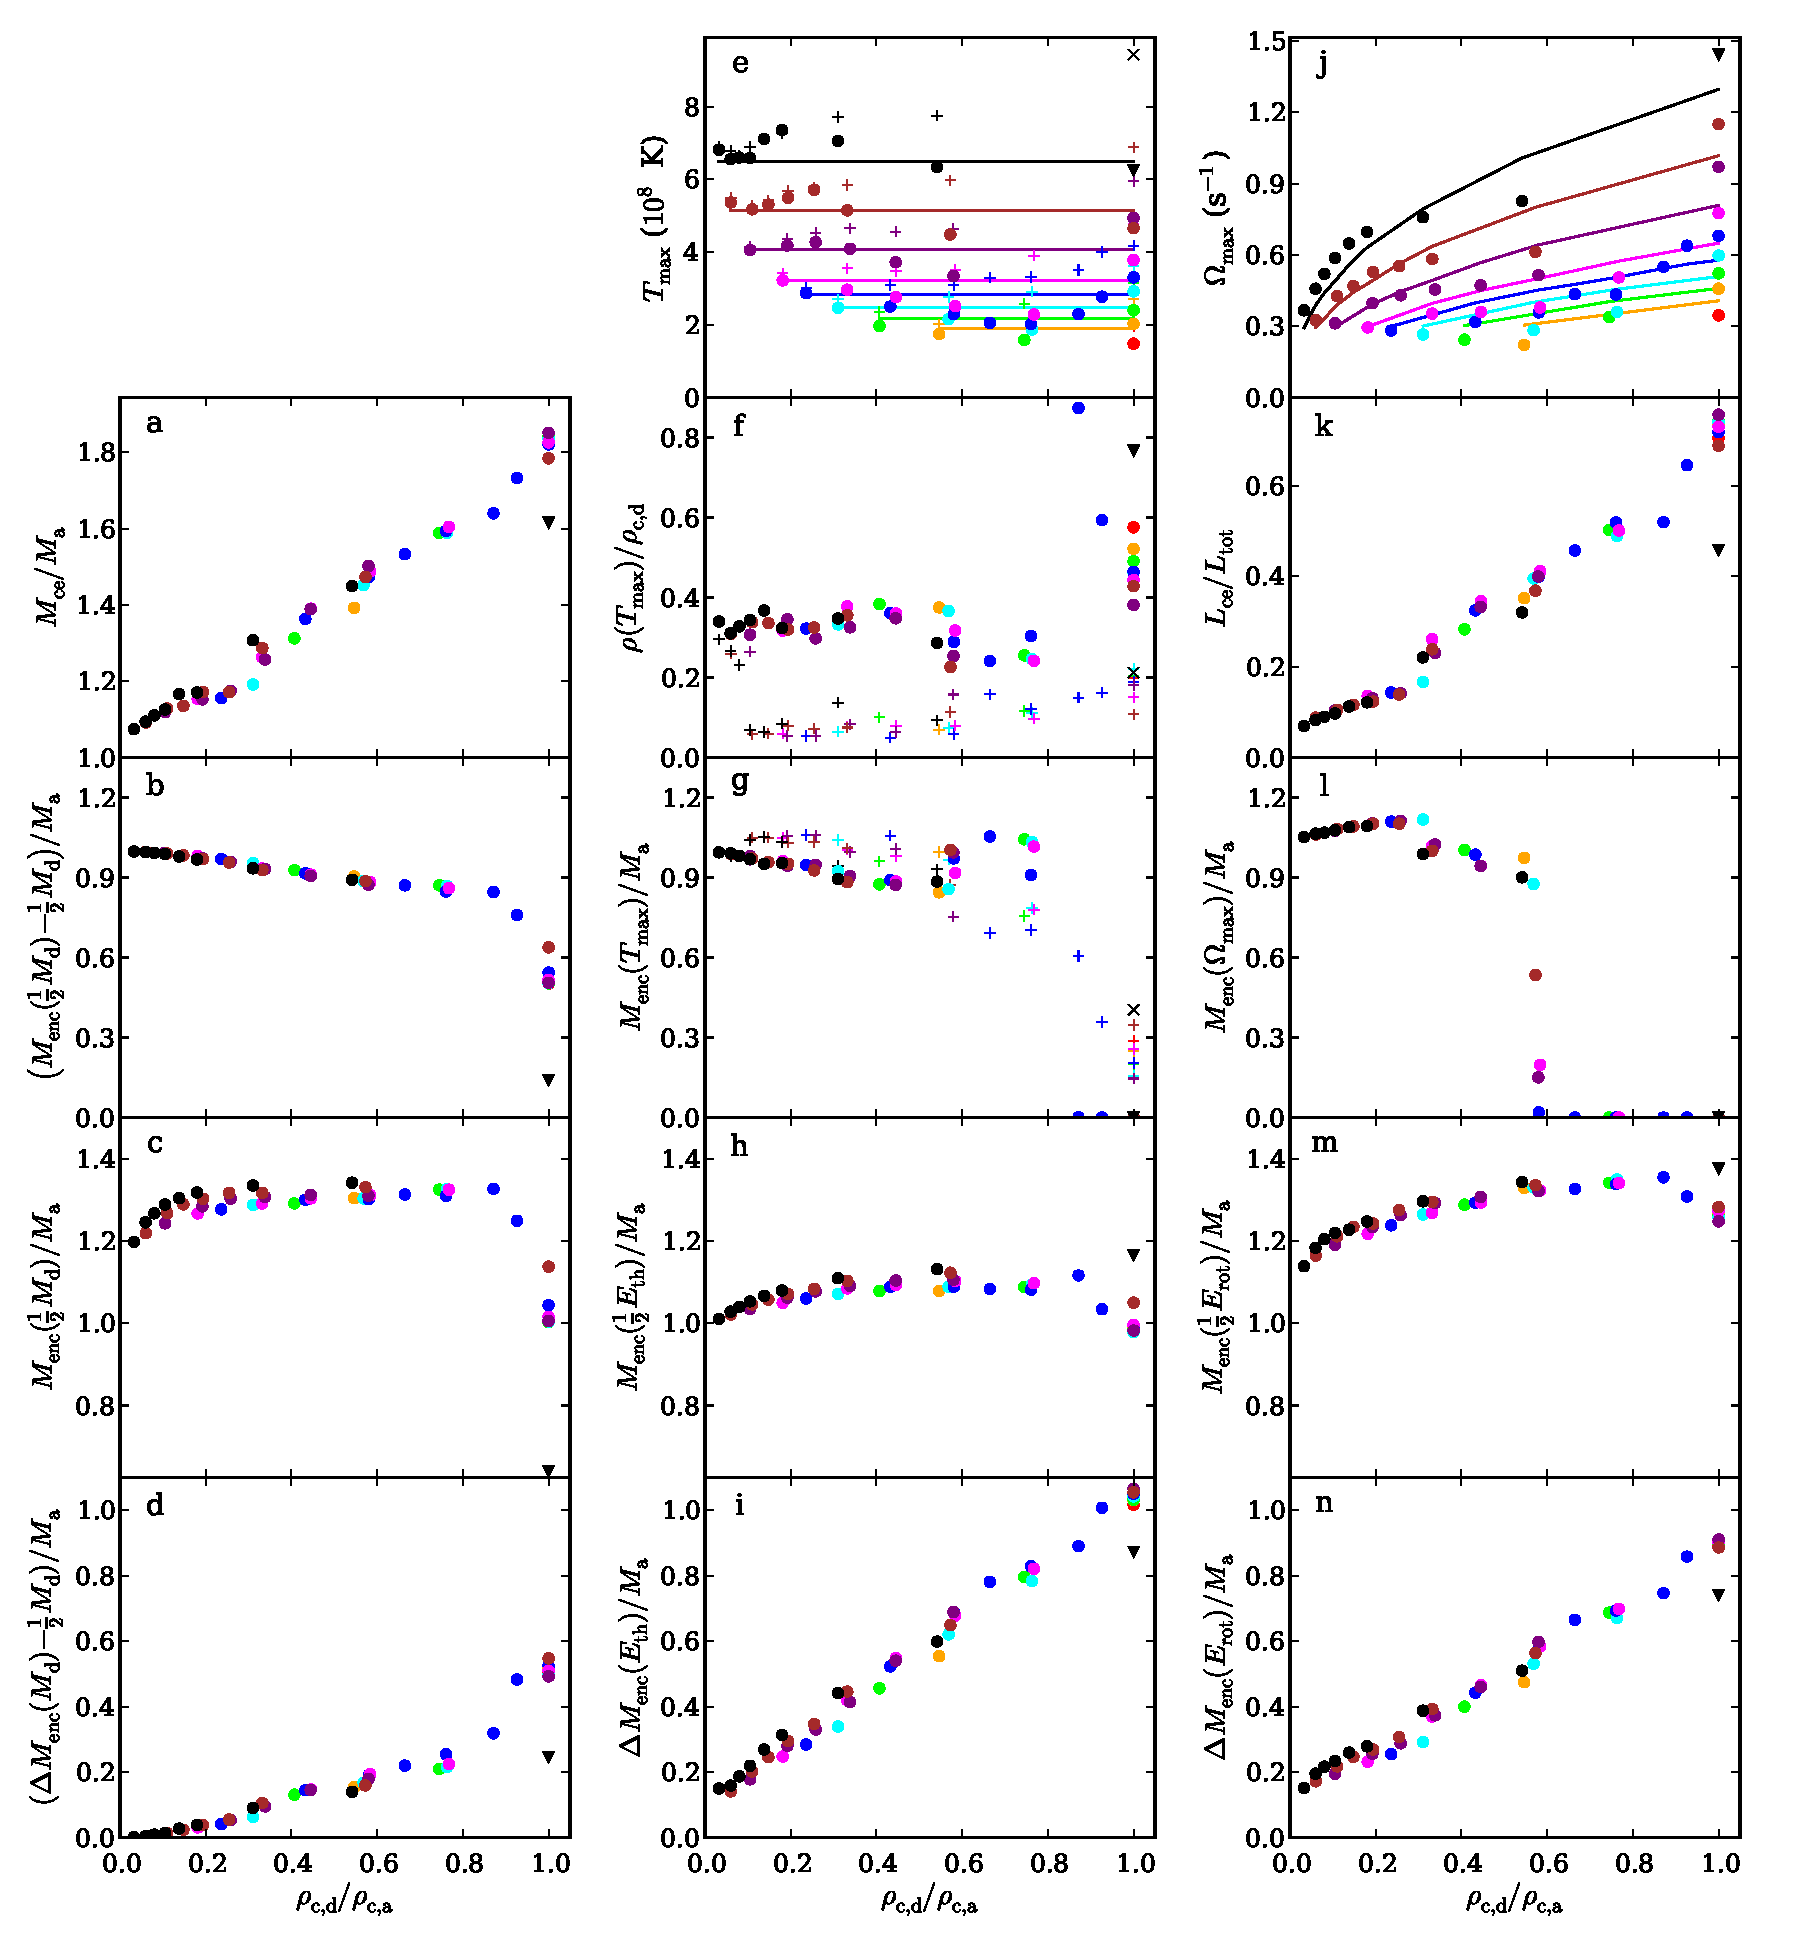
\includegraphics[angle=0,width=1.0\columnwidth]{chapter2_zhu+13/figures/RestofTrendsq.pdf}
\caption{Mixing, heating, and spin-up (left to right) for mergers. (a) Scaled mass of the remnant core-envelope (where scaling here and below is to the accretor mass).  (b) Fraction of the accretor within the mass enclosing half the donor mass.  (c) Scaled remnant mass enclosing half the donor mass.  (d) Fraction of the accretor mass within the region enclosing 25--75\% of the donor mass.  (e) Maximum equatorial temperature \Tmax\ (circles), with the approximation $\Tmax=0.20G\Ma m_\mathrm{p}/k_B\Ra$ overdrawn.  Maximum temperatures along the rotational axis are shown with crosses.  (f) Scaled density at the location of \Tmax\ (symbols as above).  (g) Scaled mass enclosed within the radius of \Tmax\ (symbols as above).  (h) Scaled mass enclosing half of the remnant thermal energy.  (i) Scaled mass of the region enclosing 25 -- 75\% of the remnant thermal energy.  (j) Maximum angular velocity \Omegamax\ (circles) with best fit $\Omegamax=3.8\Omega_\mrm{orb}$ overdrawn.  (k) Fraction of the angular momentum in the core-envelope.  (l) Scaled mass enclosed within the radius of maximum angular velocity.  (m) Scaled mass enclosing half of the total remnant rotational energy.  (n) Scaled mass of the region enclosing 25 -- 75\% of the remnant rotational energy.  Colors represent different accretor masses, encoded as in Fig.~\ref{fig:c2_constacc}.  Triangles represent equatorial plane values, and x-marks rotational axis values, of the 1.0 - 1.0\,\Msun\ merger.}
\label{fig:c2_restoftrends}
\end{figure*}

\subsubsection{Energy Balance}

The energy balance of the remnants indicate their primary means of support.  Since the remnants are virialized, we consider how the ratio of degeneracy, thermal, and rotational energy to the total internal energy of the remnants varies with \qrho.

\paragraph{Energy balance of the entire remnant.} The support against gravity changes from being due mostly to degeneracy pressure at low \qrho\ to having a substantial rotational contribution at $q_\rho\simeq1$.  This is because for highly dissimilar-mass mergers most of the internal energy is locked up within the accretor, which is hardly heated or spun up.  For similar-mass mergers, however, donor material mixes, to some degree, with the entire accretor, causing heating and spin-up throughout the entire remnant.

The total gravitational potential energy of the merger remnant can be described adequately by a constant fraction of $GM_\mrm{tot}^2/\Ra$,
\eqbegin
\frac{-E_\mathrm{pot}}{GM_\mrm{tot}^2/\Ra} = 0.49
\qquad(\pm0.01).
\eqend

%{\bf MHvK: I replaced the term internal energy with kinetic energy below, since it seems more appropriate; after all, molecular rotational or vibrational energy would be irrelevant.  CZ: in SPH ``kinetic'' seems to have an obvious definition, the speed of the particles, rather than the individual nuclei and electrons in the gas.  I feel the same is true for fluids in general, that the kinetic energy quantity naturally points to energy of bulk fluid flow.  I've left everything as is for now, but I feel it should be changed to internal.}

From the virial theorem, the internal energy should be related to the potential energy by $3(\langle\gamma\rangle - 1)E_\mathrm{I} = -E_\mathrm{pot}$, where $\langle\gamma\rangle$ is an appropriately averaged equivalent to the adiabatic index.  Since our remnants have cores where the electrons are becoming relativistic, one has $\langle\gamma\rangle$ somewhat smaller than $5/3$, especially for the more massive remnants.  We find that the ratio $E_\mathrm{I}/|E_\mathrm{pot}|$ can be described by,
\eqbegin
\frac{E_\mathrm{I}}{|E_\mathrm{pot}|} = 0.18\frac{M_\mathrm{a}}{M_\odot} + 0.42
\qquad(\pm0.01),
\eqend
which is $\sim$0.5 and $\sim$0.6 for low and high $M_\mathrm{a}$, respectively.  

The fraction of the internal energy carried by degeneracy and rotation is fairly well described by,
\begin{eqnarray}
\frac{E_\mathrm{rot}}{E_\mathrm{I}} &=& 0.31\qrho^{1/2}
\qquad(\pm0.01),\\
\frac{E_\mathrm{deg}}{E_\mathrm{I}} &=& 0.92 - 0.34\qrho^{1/2}
\qquad(\pm0.02).
\end{eqnarray}
With these, the fraction carried by thermal energy can also be calculated; as shown in Fig.~\ref{fig:c2_energytrends}a, the fraction in thermal energy first increases with increasing \qrho, but turns over at $\qrho\simeq0.7$, decreasing afterwards.  This reflects the competition between increased thermal energy from the two stars mixing, and increased rotational support from the spin-up of the core.  

Overall, for highly dissimilar-mass mergers, the internal energy is partitioned into degeneracy, rotational and thermal energy with a ratio of approximately 8:1:1, reflecting that, as stated above, such mergers are almost entirely supported by degeneracy pressure.  Similar-mass mergers, on the other hand, partition their internal energies with the ratio 6:3:1, i.e., rotational support is significant.  

\paragraph{Energy balance of the core-envelope.} Since the variations with \qrho\ seen for the remnant as a whole are almost entirely due to variations in the core and envelope rather than in the disk, the trends we find for the core-envelope are very similar to those we found above for the entire remnant,
\begin{eqnarray}
%\frac{-E_\mathrm{pot,ce}}{G\Ma\Md/\Ra} &=& 0.45
%\qquad(\pm0.02), \\
%\frac{E_\mathrm{I,ce}}{|E_\mathrm{pot,ce}|} &=& 0.182\frac{M_\mathrm{a}}{M_\odot} + 0.401
%\qquad(\pm0.009), \\
\frac{E^\mrm{ce}_\mathrm{rot}}{E^\mrm{ce}_\mathrm{I}} &=& 0.28\qrho
\qquad(\pm0.02), \\
\frac{E^\mrm{ce}_\mathrm{deg}}{E^\mrm{ce}_\mathrm{I}} &=& 0.94 - 0.32\qrho
\qquad(\pm0.02).
\end{eqnarray}
Note the dependency on \qrho, rather than on $\qrho^{1/2}$ as was found for the entire remnant.  See Fig.~\ref{fig:c2_energytrends}b.

\paragraph{Energy balance of the disk.} For the disk, we find very little dependence on \qrho, consistent with the idea that most of the changes in the partitioning of energy have to do with increased mixing between the donor and accretor, which affects the core and envelope much more than the disk.  Averaged over all mergers, we find
\begin{eqnarray}
\frac{E^\mrm{disk}_\mathrm{rot}}{E^\mrm{disk}_\mathrm{I}} &=& 0.74
\qquad(\pm0.03),\\
\frac{E^\mrm{disk}_\mathrm{th}}{E^\mrm{disk}_\mathrm{I}} &=& 0.19
\qquad(\pm0.02),\\
\frac{E^\mrm{disk}_\mathrm{deg}}{E^\mrm{disk}_\mathrm{I}} &=& 0.07
\qquad(\pm0.02).
\end{eqnarray}
Hence, the disk is composed of non-degenerate, primarily rotationally-supported material.  See Fig. \ref{fig:c2_energytrends}c.  (Note that we do not try to define a ratio of internal to potential energy of the disk or core-envelope, since the potential energy of either is not straightforward to determine.)

\begin{figure}
\centering
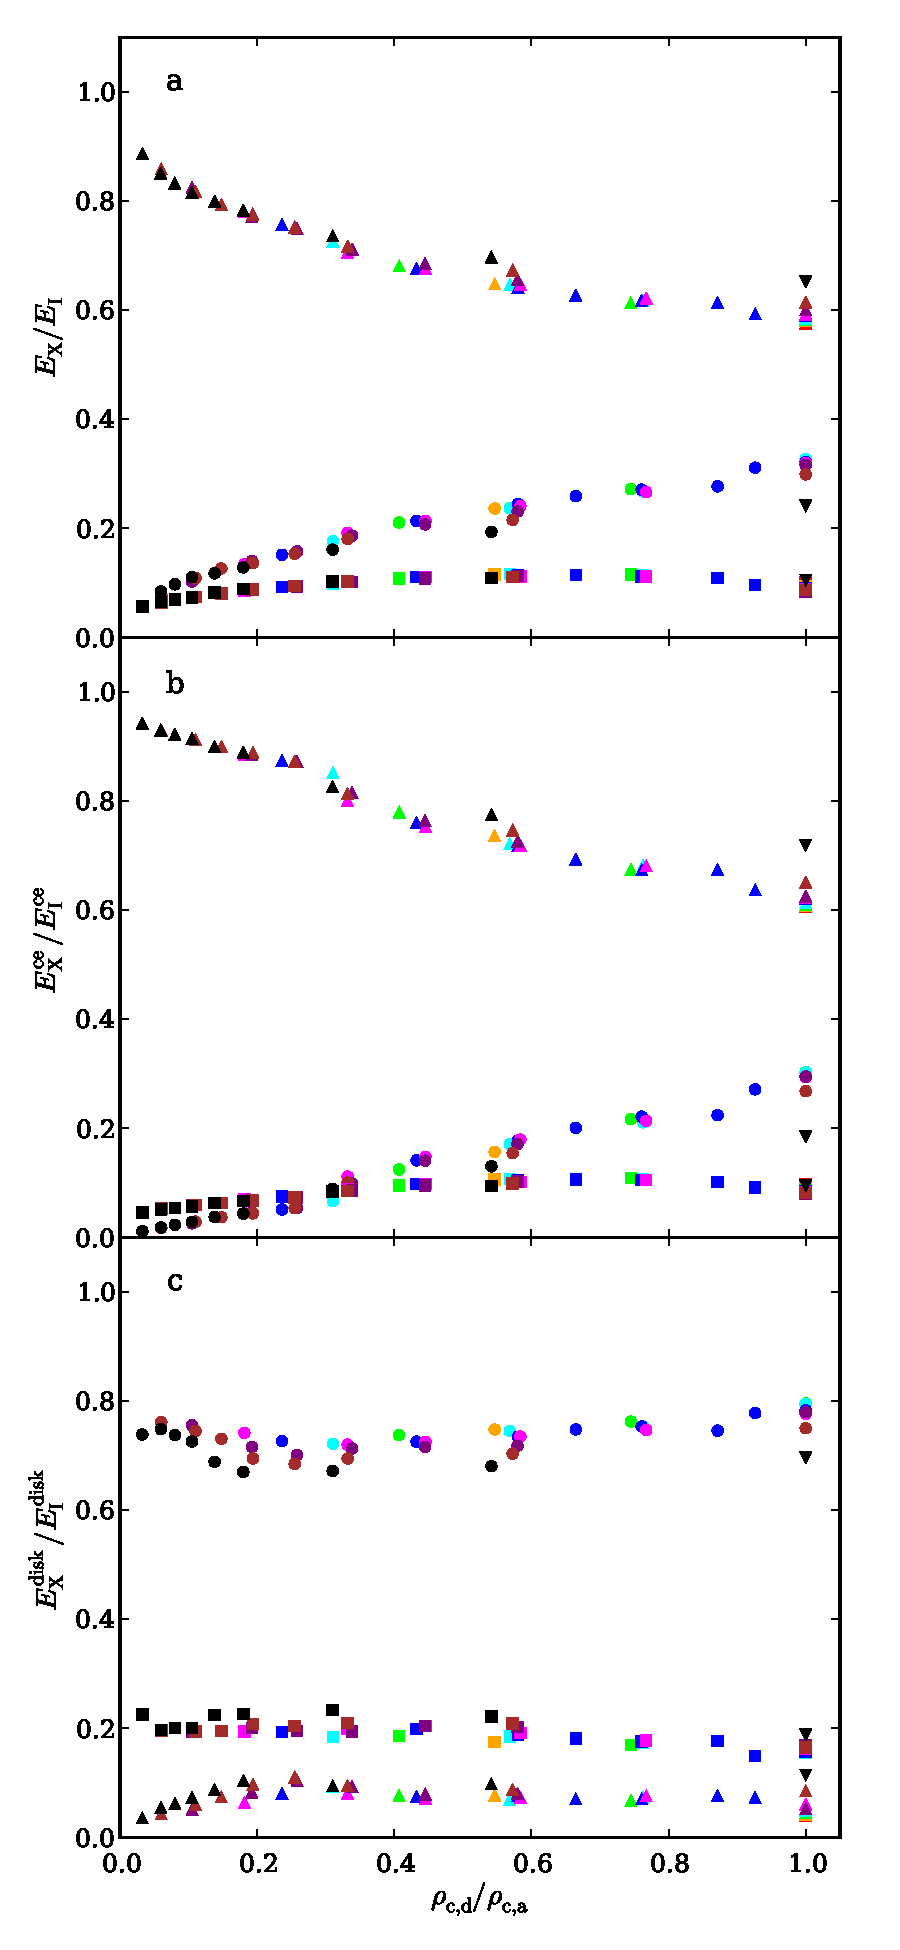
\includegraphics[width=0.6\columnwidth]{chapter2_zhu+13/figures/EnergyTrendsq.pdf}
\caption{Partition of energies in (a) the overall merger remnant, (b) the remnant core plus envelope, and (c) the remnant disk.  In each panel, the fraction of total energy carried in degeneracy (triangles), thermal (squares), and rotational (circles) energy is shown.  Colors represent different accretor masses, encoded as in Fig.~\ref{fig:c2_constacc}.  Triangles represent the 1.0 - 1.0\,\Msun\ merger.}
\label{fig:c2_energytrends}
\end{figure}

\subsubsection{Temperature and Thermal Energy}
\label{sssec:c2_thermtrends}

Since heating of the remnant is achieved through shocks and viscous dissipation, the most heavily mixed regions should also be the hottest.  We focus on equatorial thermodynamic values, but consider the rotational axis as well for similar-mass mergers.

\paragraph{The maximum temperature.} We find that the maximum temperature on the equatorial plane, \Tmax, scales with the potential of the accretor (Fig.~\ref{fig:c2_restoftrends}e),
\eqbegin
\frac{k\Tmax}{G\Ma m_\mathrm{p}/\Ra} = 0.20
\qquad(\pm0.03).
\eqend
This scaling is natural in the limit of highly dissimilar-mass merger -- for each nucleon, of order $G\Ma m_\mathrm{p}/\Ra$ is liberated and converted into thermal energy.  The temperature and thermal energy profiles in Fig.~\ref{fig:c2_constacc} show that with increasing {\qrho}, additional thermal energy is deposited into the remnant, but this energy is spread over a larger region, such that the maximum temperature remains roughly the same even as {\qrho} approaches unity.  

For a dissimilar-mass merger, the highest temperature along the rotational axis, \zTmax, is found at the tenuous outer edge of the hot envelope.  It is slightly higher than the maximum temperature found in the equatorial plane.  With increasing \qrho, however, the difference increases noticeably due to the two off-center hot spots found along the rotational axis in similar-mass mergers.  Fitting \zTmax, we find $k\zTmax/(G\Ma m_{\rm p}/\Ra) = 0.24\pm0.03$, though this does not capture the upturn for similar masses well.

All remnants with $q_\rho\gtrsim0.8$ have convectively unstable cores along the equatorial plane.  Artificially mixing these cores to make them isentropic decreases their maximum temperatures by 10 -- 50\% (not shown in Fig.~\ref{fig:c2_restoftrends}, but see the left panel of Fig.~\ref{fig:c2_willitexplode}).  All remnants are stable against convection along the rotational axis.

\paragraph{The density at the point of maximum temperature.}  For dissimilar-mass mergers, the density at the hottest equatorial point, \rhoTmax, depends mostly on the donor (see Fig.~\ref{fig:c2_restoftrends}f).  For $\qrho\lesssim0.5$, we find
\eqbegin
\frac{\rho(T_\mathrm{max})}{\rhocd} = 0.34
\qquad(\pm0.02).
\eqend
This proportionality again suggests that, at least for dissimilar-mass mergers, the donor mixes with the accretor up to a fraction of the central density of the donor, as alluded to earlier.  

At $\qrho\gtrsim0.6$, the dependence becomes less obvious, with \rhoTmax\ varying from $\sim\!25$ -- 90\% of \rhocd.  Since for these density ratios,  the donor material starts to penetrate the central core of the accretor -- and the accretor starts to disrupt as well -- the simple picture of the donor mixing up to a fraction of its own central density may be breaking down.  Furthermore, part of the spread in density reflects that for high \qrho\ the equatorial temperature profiles become nearly flat (see Fig.~\ref{fig:c2_constacc}, left column), thus increasing the sensitivity to noise in the determination of the location (but not the value) of maximum temperature.  This also affects our results for the enclosed mass, \MencTmax, below.

Since for dissimilar-mass mergers, \zTmax\ is located near the tenuous outermost regions of the hot envelope, where particle noise is high, the density at the point of maximum rotational axis temperature, \zrhoTmax\ (plus symbols in Fig. \ref{fig:c2_restoftrends}f), varies wildly between about \rhoTmax\ and one order of magnitude below \rhoTmax.  For similar-mass mergers, \zrhoTmax\ appears to be $\sim\!20$ -- 50\% of {\rhoTmax}.

\paragraph{The mass enclosed within the radius of maximum temperature.}  For dissimilar-mass mergers, the radius of maximum temperature occurs at an enclosed mass of $\MencTmax\simeq\Ma$, while for mergers with $\qrho\gtrsim0.8$, maximum temperature occurs at the center and $\MencTmax\simeq0$ (see Fig.~\ref{fig:c2_restoftrends}g).  For $\qrho\lesssim0.5$, we find
\eqbegin
\frac{\MencTmax}{\Ma} = 1-0.28\qrho
\qquad(\pm 0.01),
\eqend
where the fit's $y$-intercept is forced to unity.  Note that maximum temperature occurs near the bottom of the mixed zone, which is why \MencTmax\ is substantially smaller than \MMfifty.  The reasons it starts to deviate from a tight trend at $\qrho\simeq0.6$ are the same as those for \rhoTmax: the break-down of the simple mixing picture and the difficulty in determining the location of peak temperature for a broader plateau.

Since $\MencTmax<\Ma$, it may be surprising that \rhoTmax\ is not higher than \rhocd.  This is because the additional thermal and rotational support against gravity reduces the density gradient that would be required if degeneracy pressure were the only source of support.

For dissimilar-mass mergers, \zMencTmax\ is only slightly higher than \MencTmax, since the remnant core is nearly spherically symmetric, apart from the fact that the hot envelope is slightly more extended in the vertical direction.  For similar-mass mergers, the difference increases, reflecting the development of the off-center hot spots, until $\zMencTmax/\Ma\simeq0.25$ for equal-mass mergers.

\paragraph{The mass enclosing half the remnant thermal energy.}  As a more robust measure of where thermal energy is deposited during the merger, we consider the mass enclosing half the remnant thermal energy, \MEthermfifty\ (see Fig.~\ref{fig:c2_restoftrends}h).  We find this is very close to the mass of the accretor,
\eqbegin
\frac{\MEthermfifty}{\Ma}= 1.06
\qquad(\pm 0.04),
\eqend
if the 1.0 - 1.0 {\Msun} merger is neglected.  One sees turnovers at the extremes, for $\qrho\lesssim0.2$ and $\qrho\gtrsim0.8$.  The former likely is because thermal energy is deposited into a narrow strip right on the surface of the accretor, while the latter is probably due to the disruption of the accretor.

While smaller than \MMfifty, \MEthermfifty\ is always larger than \MencTmax.  This reflects that high density degenerate material has lower specific heat, so that for the same energy per unit mass the temperature is higher (see Fig.~\ref{fig:c2_constacc}).  

\paragraph{The width of the remnant thermal energy.}  The mass enclosed between the 25$^{\rm th}$ and 75$^{\rm th}$ percentiles of thermal energy, $\MEthermthick = M_{\rm enc}(\frac{3}{4}E_\mathrm{th}) - M_{\rm enc}(\frac{1}{4}E_\mathrm{th})$, is a measure of the extent of the remnant that has been heated (see Fig.~\ref{fig:c2_restoftrends}i).  Ignoring the 1.0 - 1.0 \Msun\ merger, it can be fit by,
\eqbegin
\frac{\MEthermthick}{\Ma} = 0.11+0.94\qrho
\qquad(\pm0.03).
\eqend
Here, we did not force the $y$-intercept to go to zero, which is expected physically but gives a substantially poorer trend.

%{\bf MHvK: please clarify the next sentence; what is the point?} {\MEthermthick} is also about \emph{DOUBLE???} the width of the ``bumps'' of high temperature seen in Fig.~\ref{fig:c2_constacc}.  

%\textbf{I don't think the 0.306 is physical.  For a zero-mass donor, {\MEthermthick} is non-zero (it doesn't matter how much thermal energy the accretor has, {\MEthermthick} will be non-zero), but describes something totally different than {\MEthermthick} during a merger.  Supposedly there's a transition zone between the zero-mass donor and our regime, where it describes the temperature bump, but since we have no data on this we can't say anything about this zone.  0.281, then isn't anything more than a way to make this section of the trend fit, and doesn't represent {\MEthermthick} for a zero-mass donor.}

%\begin{figure}
%\centering
%\includegraphics[angle=0,width=0.7\columnwidth]{ThermTrendsq.pdf}
%\caption{Top left: maximum equatorial temperature {\Tmax} with best fit {\Tmax} = $0.202GM_\mathrm{a}m_\mathrm{p}/(R_\mathrm{a}k_B)$.  Top right: equatorial density at the point where {\Tmax} occurs, {\rhoTmax}.  Middle left: mass enclosed within the radius containing {\Tmax}, {\MencTmax}.  Middle right: mass enclosing half of the remnant thermal energy scaled to the accretor mass, {\MEthermfifty}.  Bottom left: width of the remnant thermal energy $\Delta M(E_\mathrm{therm})$ normalized by the accretor mass.  Plus symbols represent values on the $z$-axis.  Colors (Fig. \ref{fig:c2_constacc} caption) represent different accretor masses.  Upside-down triangles and x symbols represent points on the $xy$-plane and $z$-axis, respectively, that are likely outliers; in particular the ``tails'' of the {\MEthermfifty} and $\Delta M(E_\mathrm{therm})$ plots are probably due to spurious heating.}
%\label{fig:c2_thermtrends}
%\end{figure}

\subsubsection{Angular Velocity and Rotational Energy}
\label{sssec:c2_rottrends}

For a dissimilar-mass merger, the donor carries most of the angular momentum.  As a result, the hot envelope contains more angular momentum and features higher angular velocities than the core, since the envelope is where most of the accreted donor material resides.  Spin-up of the accretor is accomplished through shocks, $PdV$ work and shearing forces.  For a similar-mass merger, the two stars carry similar amounts of angular momentum and thoroughly mix.  Conservation of angular momentum then implies that the entire remnant rotates rapidly.

\paragraph{The maximum angular velocity.}  On the equatorial plane, the highest angular velocity, \Omegamax, scales linearly with the orbital angular velocity of the pre-merger binary, $\Omegaorb = 2\pi/P_\mrm{orb}$ (see Fig.~\ref{fig:c2_restoftrends}j),
\eqbegin
\frac{\Omegamax}{\Omegaorb} = 3.8
\qquad(\pm0.6).
\eqend

\paragraph{The ratio of core-envelope to total angular momentum.} For more similar-mass mergers, more angular momentum is deposited in the accretor and ends up in the core and envelope (see Fig.~\ref{fig:c2_restoftrends}k).  The ratio of core-envelope to total angular momentum, \Lrat, is approximately,
\eqbegin
\frac{L_\mrm{ce}}{L_\mrm{tot}} = 0.70\qrho
\qquad(\pm 0.03),
\eqend
where we fit only for $\qrho > 0.25$ and ignore the 1.0 - 1.0 {\Msun} merger.  For $\qrho\lesssim0.25$, the trend becomes shallower, resulting in a non-zero intercept.  This suggests that even in cases where the donor has negligible mass some angular momentum is transferred to the accretor.

\paragraph{The mass enclosed inside the radius of maximum angular velocity.}  
%MHvK: don't like this trend at all!
%\eqbegin
%\M_\mathrm{enc}(\Omega_\mathrm{max}) = 1.25(M_\mrm{a} - \frac{1}{4}M_\mrm{d})\,%\,(\pm0.04)
%\eqend
%\noindent for $q_\rho < 0.55$.  
For dissimilar-mass mergers, both \MencOmax\ and \MencTmax\ are about equal to \Ma, with \MencOmax\ slightly larger than \MencTmax: for $\qrho\lesssim0.55$, $\MencOmax/\Ma\,=\,1.05\pm0.06$.  This is consistent with the idea that the hottest and most spun-up regions are those where the donor mixed most strongly with the accretor.  For $\qrho\simeq0.6$, the off-center angular velocity peak is replaced by a plateau, and \MencOmax\ becomes ill-defined; for even larger \qrho, the highest velocities occur in the center, and $\MencOmax\simeq0$.  See Fig.~\ref{fig:c2_restoftrends}l.

%If there was no viscous redistribution of angular momentum, we would expect {\MencOmax} to equal {\Ma}, since conservation of angular momentum would require the interior donor material to have the highest angular velocity.  Since angular momentum is redistributed due to mixing during merger, {\MencOmax} moves inward slightly as {\qrho} increases.  Angular momentum is also redistributed by viscous diffusion after the merger; this effect also benefits from greater mixing, giving more equal mass mergers greater core spin-up, until {\Omegamax} no longer has a well defined position.
%\textbf{I'm actually unsure if {\MencOmax} moves inward because mixing grants more efficient transfer of angular momentum, or because for more equal mass mergers the accretor begins to acquire more angular momentum.}
%\textbf{{\Ma} actually works a little better here.  Everything I do works a bit better if the y-intercept isn't zero.}  Like for {\MencTmax}, we expect maximum mixing to be associated with maximum spin-up, and this is the case: 1.32({\Ma} - $\frac{1}{4}${\Md}) is equivalent to 0.969({\Mc}$ + \frac{1}{2}(M_\mathrm{tot} -${\Mc}).

\paragraph{The mass enclosing half the remnant rotational energy.} Like for the thermal energy, for very dissimilar masses, the mass enclosing half the rotational energy, \MErotfifty, is similar to the accretor mass (see Fig.~\ref{fig:c2_restoftrends}m).  For $\qrho\lesssim0.8$, we find
\eqbegin
\frac{\MErotfifty}{\Ma} = 1.12+0.27\qrho^{1/2}
\qquad(\pm0.01)
\eqend
Note that unlike {\MencOmax}, \MErotfifty\ continues to increase with \qrho\ (except for exactly equal-mass mergers), a consequence of particles with lower angular velocity but large lever arm that carry substantial rotational energy (see Fig.~\ref{fig:c2_constacc}).  Near $\qrho\simeq0.8$, the trend breaks as both stars are significantly disrupted.  However, even exactly equal-mass mergers have more of their rotational energy stored in the outskirts (otherwise one would have $\MErotfifty/\Ma\simeq1$).  

\paragraph{The width of the remnant rotational energy.}  We measure the extent to which the remnant is affected by spin-up through the difference between the masses enclosing 25 and 75\% of the rotational energy, $\MErotthick = M_{\rm enc}(\frac{3}{4}E_\mathrm{rot}) - M_{\rm enc}(\frac{1}{4}E_\mathrm{rot})$ (see Fig.~\ref{fig:c2_restoftrends}n).  Ignoring the 1.0 - 1.0 {\Msun} merger, it is well-described by,
\eqbegin
\frac{\MErotthick}{\Ma} = 0.12+0.77\qrho
\qquad(\pm0.03).
\eqend
Like for the thermal energy, one sees that for more similar-mass mergers, rotational energy is spread more widely throughout the remnant.

%\textbf{An alternate picture of why equal mass mergers have highest $\Omega$ at their center: during the merger of an equal mass binary both stars disrupt simultaneously, funneling material through their L1 points.  Both streams overshoot due to the asynchronisity of the binary, and end up colliding with each other.  Due to conservation of angular momentum for those individual particles (the $L$ diffusion timescale is longer than it takes for both to disrupt), they are moving with much higher $\Omega$ than at the start of merger.  As the remnant is formed, this material begins to interact with the material around it and spin down, but before much of that occurs axisymmetry is achieved and we call the merger ``complete''.  It's interesting to note that Loren-Aguilar et al. took 514 s to call their equal mass merger complete, while in our case (see the Big Chart) it's always the case that equal mass mergers take the least amount of time to equilibrate.  This bias might be because a light WD has trouble ``smearing out'' into a torus, while equal mass mergers have no such problem, or just because the symmetry of masses makes the system more symmetric in general.  Marten suggested that we switch to outputting all our mergers after $X$ number of orbits - this might be a good idea, though it would require we rewrite a lot of things.}

%\begin{figure}
%\centering
%\includegraphics[angle=0,width=0.7\columnwidth]{RotTrendsq.pdf}
%\caption{Top left: maximum (cylindrically averaged) angular velocity {\Omegamax} with best fit $\Omega_\mrm{max} = 3.56\Omega_\mrm{orb}$, where {\Omegaorb} is the orbital angular velocity of the pre-merger binary.  Top right: ratio of remnant to total angular momentum {\Lrat}.  Middle left: enclosed mass inside the radius of maximum angular velocity {\MencOmax}.  Middle right: mass enclosing half of the total remnant rotational energ {\MErotfifty}.  Lower left: width of the remnant rotational energy scaled with the accretor mass $\Delta M(E_\mathrm{rot})$/{\Ma}.  Colors (Fig. \ref{fig:c2_constacc} caption) represent different accretor masses.  Upside-down triangles represent points that are likely outliers.}
%\label{fig:c2_rottrends}
%\end{figure}

\subsection{A Qualitative Picture of the Merger}
\label{ssec:c2_qualitative}

From our empirical results above, a qualitative picture of a merger emerges.  A dissimilar-mass merger has the donor overflowing its Roche lobe and forming an accretion stream.  This stream mixes with the accretor up to approximately the central density of the donor pre-merger, \rhocd.  Those layers of the accretor that are denser than \rhocd\ are hardly affected, and form the cold core of the merger remnant, while the mixed material will form a partly-thermally supported outer envelope, which somewhat compresses the core, as well as a rotationally supported disk.

At $\qrho\gtrsim0.6$, the above picture begins to break down, as portions of the donor start to penetrate to the center of the accretor.  This results in substantial heating and spin-up of the central core: the merger becomes a similar-mass merger.  As the masses become more similar, the distinction between donor and accretor is lost and both stars disrupt and form accretion streams.  For all $\qrho\gtrsim0.6$, the remnants are similar: a large, ellipsoidal and partly rotationally supported hot core with two hotspots off the equatorial plane, surrounded by a small, hot disk.

For all mergers, the maximum temperature reached by dissipation of orbital energy is proportional to the accretor's gravitational potential energy.  For increasing \qrho, the maximum temperature remains similar, but the region over which the thermal energy is deposited widens.  The density at maximum temperature is of the same order of magnitude as the central density of the donor, consistent with the mixing picture discussed above.  The latter no longer holds for $\qrho\gtrsim0.6$, when the entire remnant is mixed and heated.

For a dissimilar-mass merger, the angular momentum remains in the outer regions, since most of it was originally carried by the donor.  Angular momentum can be transferred between regions through shocks, $PdV$ work or shearing forces, all of which becomes increasingly important as the donor penetrates deeper.  As a result, with increasing \qrho, the remnant core is spun up further.  Where both WDs disrupt, leading to colliding accretion streams, even the densest regions of the remnant have high rotational velocities.

%Spin-up, which is also due to mixing, occurs in approximately the same region as heating (it is slightly outward), and for unequal mass mergers this is a very small region.  As mixing increases, the increase in angular velocity of the core does also, though {\Omegamax} increases slowly.  For unequal mass mergers thermal and Fermi pressure dominate over rotation in dictating the overall structure of the remnant core.  As {\qrho} increases the spin-up of the core results in rotation playing a greater role in determining the structure of the core.  For an equal mass merger, rotation support dominates greatly over thermal support.

%\textbf{ Why does the thermal energy dumped into the system DROP as the merger becomes more equal mass (this is not totally obvious from the figures in the paper due to normalization of the x-axis, but it's obvious from the big output chart when plotting Etherm for the total remnant)?  Since mixing presumably means more thermal energy generation, I would expect the total thermal energy to increase, even if the rotational energy increased more.  What sets how much heating the remnant receives?  This issue may be related to why our Omega curves for equal mass mergers look totally different than other people's, which is our remnant has yet to "finish" evolving - the center has yet to spin down, which would generate more heat for the remnant.  If this were the case, the energy balance oddity might disappear (or at least diminish), but at the same time Omega will no longer look different for equal mass mergers than sort of equal mass mergers (i.e. they'll all just have a plateau), and rotation would play a less prominent role in the remnant.  This would weaken the case for equal mass mergers being a separate class of mergers since there would be a smoother evolution of remnant properties from unequal to equal masses.}


\section{Variation of Merger Parameters and Robustness of Results}
\label{sec:variation}

In our parameter space study, we focused on the effects of varying the masses of the two WDs, fixing the initial separation {\azero}, merger completion time criterion, and WD composition.  To determine how robust our results are, we ran simulations varying these assumptions.

\subsection{Changing the Composition}

\begin{figure}
\centering
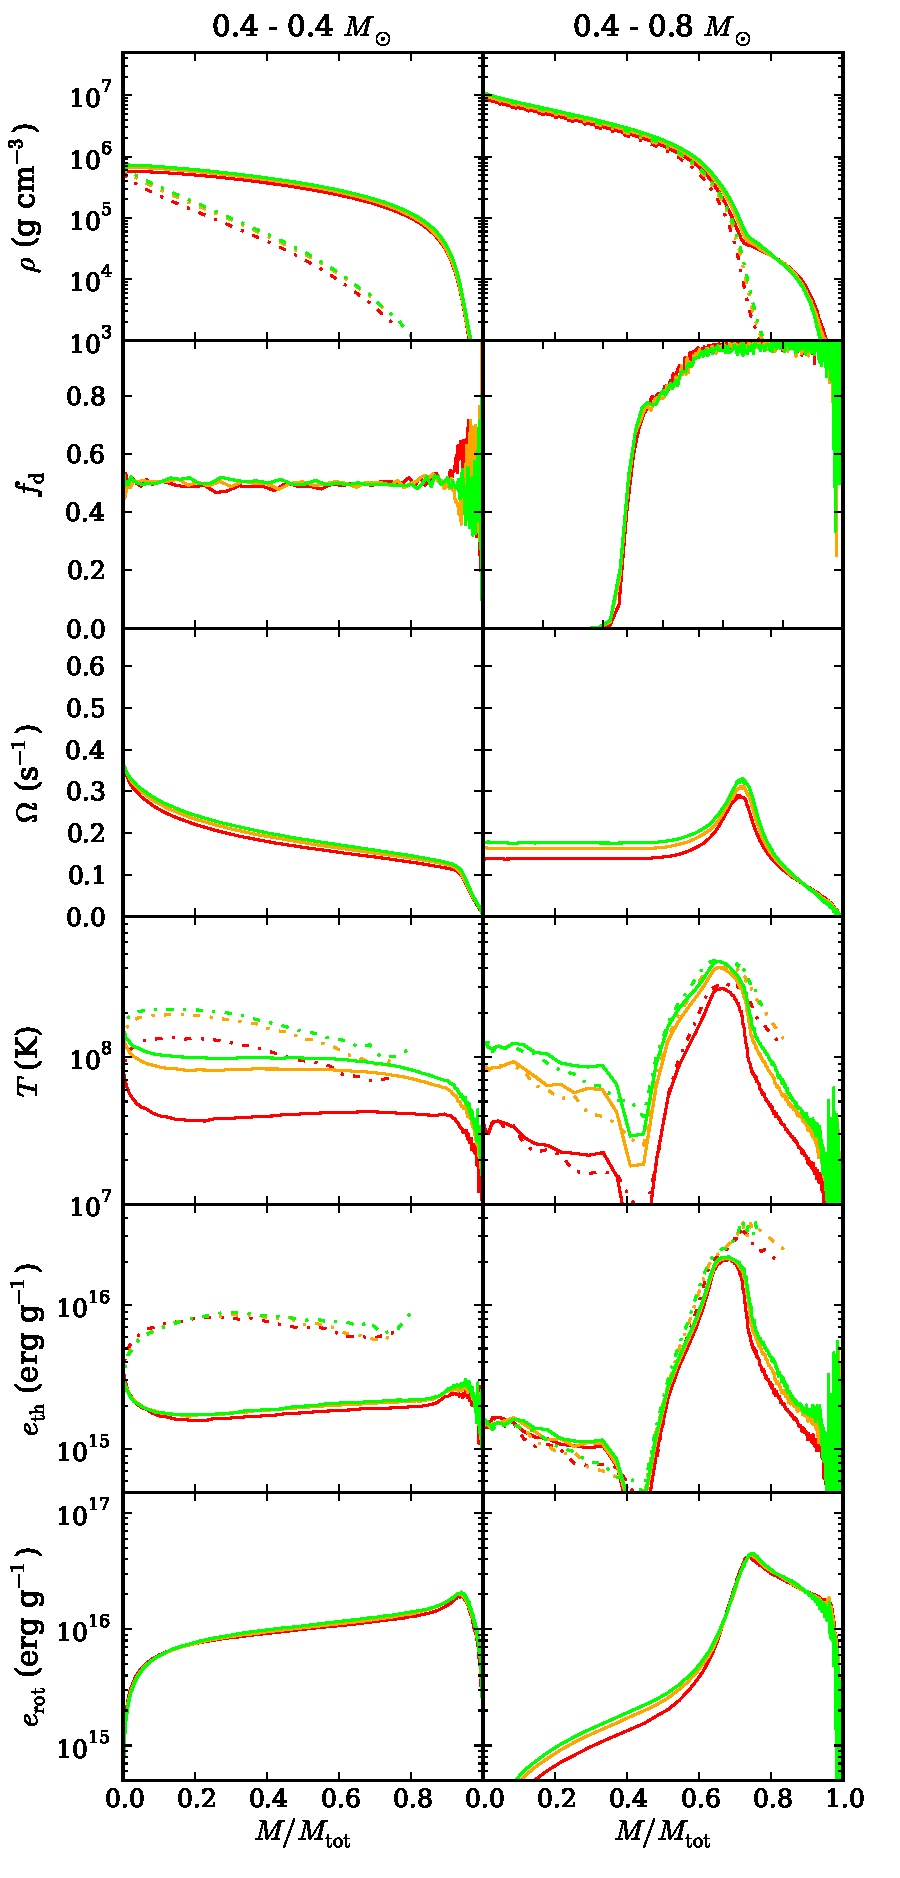
\includegraphics[angle=0,width=1.0\columnwidth]{compcomp.pdf}
\caption{As Fig.~\ref{fig:constacc}, but for 0.4 - 0.4 {\Msun} (left) and 0.4 - 0.8 {\Msun} (right) mergers with different compositions: pure $^4$He (red), CO (orange), and pure $^{24}$Mg (lime).  Dash-dotted lines represent profiles along the rotational axis rather than the equatorial plane.}
\label{fig:compcomp}
\end{figure}

Ignoring fusion, WD mergers should be insensitive to changes in composition, since the dominant electron degeneracy pressure only depends on the mean molecular weight per electron, which is close to $\mu_e\simeq2$ for all likely compositions.  To confirm this, we ran simulations assuming pure helium and pure magnesium for an equal-mass case (0.4 - 0.4\,\Msun) and an dissimilar one (0.4 - 0.8\,\Msun).  The results are shown in Figure \ref{fig:compcomp}.  One sees that most quantities indeed have very similar profiles.

The set of profiles showing most variation are those of the temperature.  These have similar shape, but different normalization.  Since the thermal energy curves are very similar, it is clear that this reflects differences in heat capacity, which does depend on composition: for He composition, there are more (non-degenerate) ions than for our standard CO mixture, boosting the heat capacity (and thus lowering the temperature for given thermal energy), while for Mg composition, there are fewer, lowering the heat capacity (and increasing the temperature).  As a result, the maximum equatorial plane temperatures for the 0.4 - 0.4\,\Msun\ simulations are 0.95, 1.48 and $1.68\times10^8$ K for He, CO, and Mg, respectively, while for the 0.4 - 0.8\,\Msun\ simulations, they are 2.92, 4.05, and $4.47\times10^8\,$K.

%MHvK: with changes to above paragraph, this one became superfluous.
%A comparison of the specific thermal energy profiles hammers home this point.  Here, the thermal energy profiles, $E_{\rm therm}$ are nearly identical for the different compositions.  In particular, for the $0.4\,-\,0.8\,M_\odot$ simulations we find maximum thermal energies of $2.1\times10^{16}{\rm\,erg\,g^{-1}}$ with a deviation of about 4\%, while in the $0.4\,-\,0.4\,M_\odot$ simulations we find maximum thermal energies of $3.7\times10^15{\rm\,erg\,g^{-1}}$ with a deviation of about 10\%.  The well behaved nature of our results to variations in composition, while not realistic in nature, demonstrates that the properties of WD mergers is fairly well-understood.

The smaller differences seen for the other profiles reflect small differences in initial conditions.  All WDs are constructed assuming $T=5\times10^6\,$K throughout, which implies more thermal energy for higher heat capacity.  As a result, the relaxed He and Mg WDs are slightly larger and smaller, respectively, than the CO WD.  These slight differences in radius translate into differences in initial separation, which in turn cause small differences in the angular velocity and rotational energy curves.

\subsection{Varying the Initial Binary Separation}
\label{ssec:varyingazero}

\begin{figure}
\centering
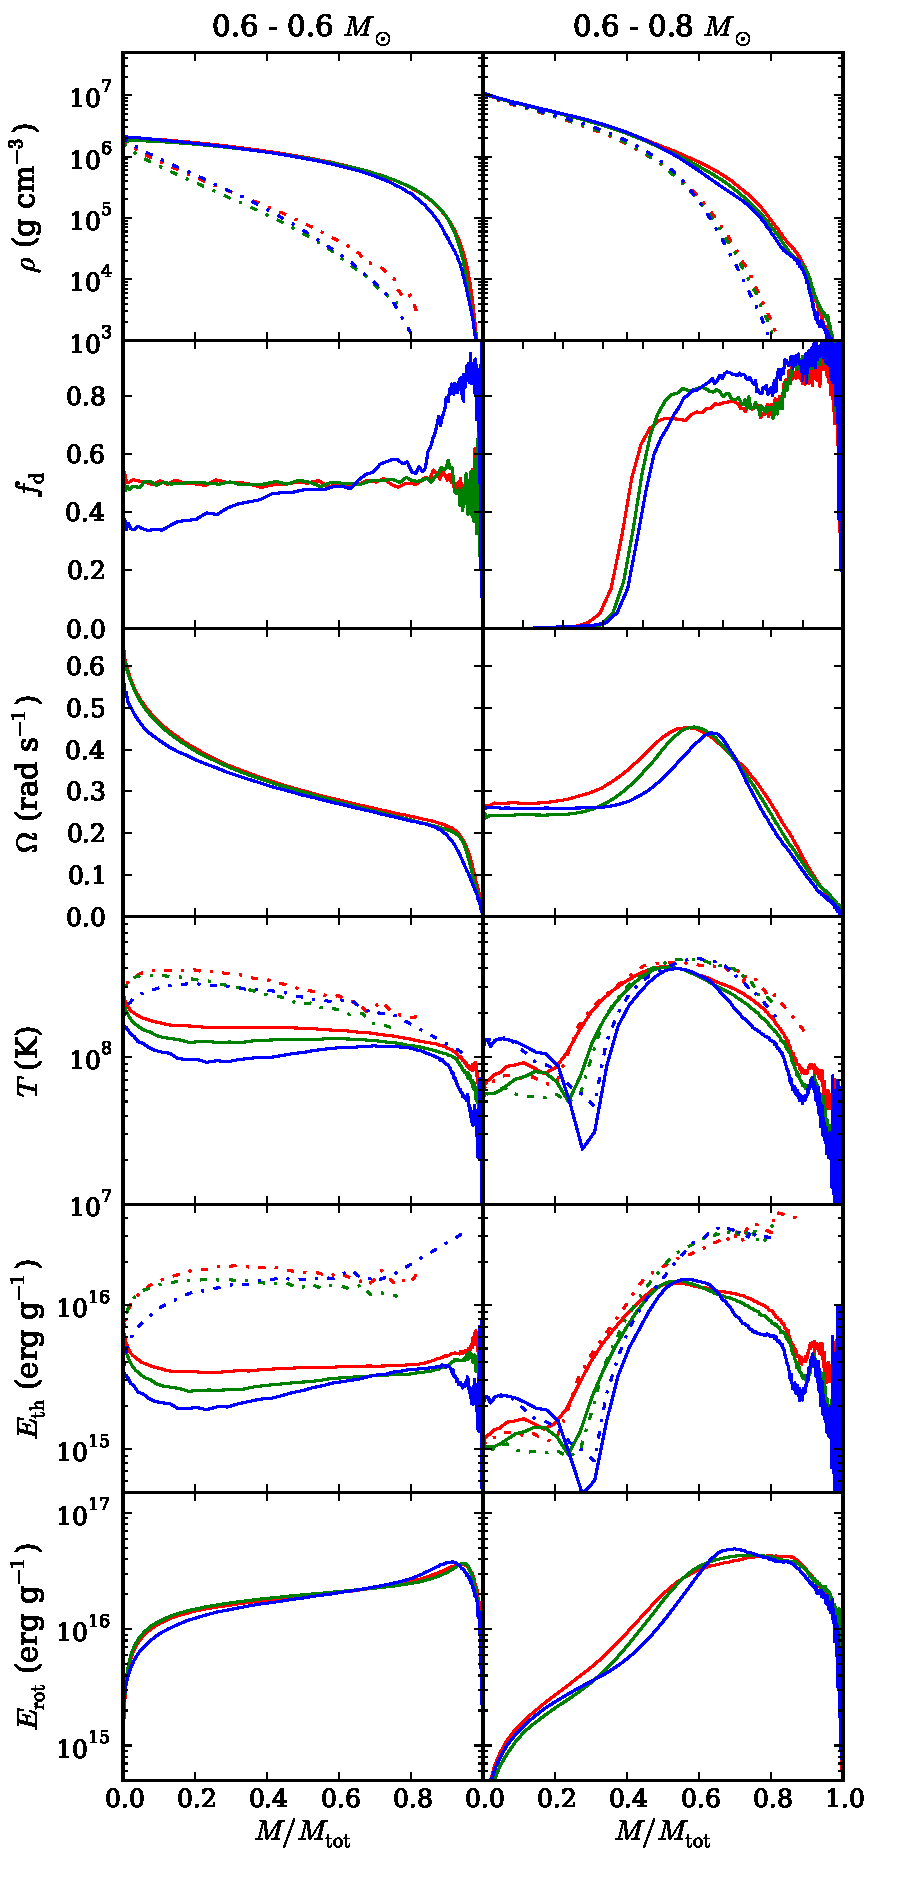
\includegraphics[angle=0,width=1.0\columnwidth]{distcomp.pdf}
\caption{As Fig.~\ref{fig:compcomp}, but for 0.6 - 0.6 {\Msun} (left) and 0.6 - 0.8 {\Msun} (right) mergers with varying initial orbital separation: 0.9 (red), 1.0 (green), and 1.1 (blue) times the value used for the parameter space study.}
\label{fig:distcomp}
\end{figure}

For our simulations, we chose an initial orbital separation {\azero} for which a co-rotating donor would fill its Roche lobe.  Since our (non-rotating) WDs are equilibrated in isolation, once the simulation starts they immediately begin to adjust to the tides and hence disrupt quickly.  Ideally, one would allow them to adjust to the binary potential and start mass transfer properly.  For non-synchronous rotation, however, this is not straightforward (see Sec.~\ref{ssec:compwithothers}).  Nevertheless, we try to get a sense of the influence of this by running simulations for two cases -- 0.6 - 0.6\,\Msun\ and 0.6 - 0.8\,\Msun\ -- with \azero\ increased and decreased by 10\% (see Fig.~\ref{fig:distcomp}).

Our default simulations were considered complete at 6 orbits of the initial binary.  For runs where \azero\ was changed, we used 2.5\% non-axisymmetry, and a requirement for the density to be highest at the remnant's center, as the completion criteria\footnote{The 2.5\% non-axisymmetry convergence time is 312 s (6.6 orbits) for our default 0.6 - 0.6 {\Msun} run, and 250 s (5.2 orbits) for our default 0.6 - 0.8 {\Msun} run.}.  Not surprisingly, runs with larger {\azero} needed longer to achieve these criteria: with a 10\% increase, the 0.6 - 0.8 {\Msun} merger required 861 seconds, or $\sim\!15$ orbits, to complete, while the one with a 10\% decrease required 230 s, or $\sim\!5.5$ orbits.  Similarly, the 0.6 - 0.6 {\Msun} merger with a 10\% increase in {\azero} required $\sim\!13$ orbits (725 s) to complete, compared to the 7 orbits of a 10\% decrease (283 s).  In both cases, the increase simply reflects that it takes longer for the donor to be disrupted fully if \azero\ is increased\footnote{Of course, if placed far enough, the binary does not merge.  For a 0.6 - 0.8 {\Msun} binary, no mass transfer occurred within 500 s if \azero\ was increased by 20\%.}.  For instance, for the 0.6 - 0.8 {\Msun} binary with increased separation, it took almost a dozen orbits before full disruption, while at the standard separation disruption occurred after just 1.5 orbits.  This feature is of particular interest because for mergers of synchronously rotating WDs \cite{dan+11,dan+12} and \cite{rask+12} all note almost immediate disruption of the donor when approximate initial conditions are used, and much delayed disruption for more accurate initial conditions (up to $\sim\!30$ orbits; see Sec.~\ref{ssec:compwithothers}).

We find that the density profiles of the merger remnants are remarkably insensitive to varying \azero\ (\rhoc\ changing by $\lesssim2$\% for the 0.6 - 0.8 {\Msun} merger, and $\sim20$\% for the 0.6 - 0.6 {\Msun} merger), and show substantial systematic changes only in the outer regions.  The latter can be understood from the mixing and rotational profiles, where one sees that with increasing \azero, donor material is mixed less deeply into the accretor, and rotational energy is shifted outward, causing the rotational frequency to peak at lower values and larger radii.  This reflects the increase in angular momentum with increasing \azero, which creates a more rotationally supported remnant (for both our systems, a 10\% increase (decrease) in \azero\ results in a 5\% increase (decrease) in angular momentum).  In the 0.6 - 0.8\,\Msun\ merger, the decreased mixing causes the accretor to be spun up less, thus lowering the rotational energy of the core, and narrowing the thermal energy plateau.  These effects are also seen in the similar-mass case, where the center of the remnant receives less rotational support and becomes denser with increasing separation, and the mixing becomes less uniform.

Qualitatively, with increasing \azero, the properties change in a way that is similar to the changes seen with decreasing \qrho, i.e., similar to mergers with more dissimilar mass: reduced mixing, larger disks and less core rotational support, and shifts in the thermal and rotational energies toward larger radii.  The converse is also true, decreasing \azero\ has similar effects as increasing \qrho, i.e., the mergers become similar to those with more equal masses.  The changes are substantial at times: e.g. with a 10\% increase in {\azero} for the 0.6 - 0.6 {\Msun} remnant, the maximum equatorial temperature is reduced by 40\%, while the corresponding density increases by 25\% (for the rotational axis hotspots, the values are a 13\% and 30\% reduction, respectively), and the mass of the disk increases by 65\%.  Similar, though far less extreme, changes are seen for the properties of the 0.6 - 0.8 {\Msun} remnant.  All this makes {\azero} one of the parameters our mergers are most sensitive to.

%For a 10\% change in \azero, many remnant properties change substantially: e.g., {\rhoTmax} changes by $\sim\!15$\% for both mergers, while {\Tmax} decreases by 35\% for the 0.6 - 0.6\,\Msun\ merger when {\azero} is increased by 10\% (along the equatorial plane, along the rotational axis, the decrease in temperature is $\sim10$\%, and density $\sim30$\%).  For the 0.6 - 0.6 \Msun\ merger, the mass of the (very small) disk increased by 65\% for the 10\% increase in \azero, while for the 0.6 - 0.8\,\Msun\ merger, the effect was around 4\%.  Thermodynamic properties around temperature maxima are in general more robust to changes in {\azero} for the 0.6 - 0.8\,\Msun\ merger than in the 0.6 - 0.6 \Msun\ merger, while the reverse is true for core-envelope energy and angular momentum.  {\bf CZ: does this paragraph have any use??}

%CZ: This is not true (and you can tell from the figure that the equal mass and unequal mass mergers both change substantially)!!!
%In general, the similar-mass merger changed more drastically than the unequal mass one: for the former, only the central scale height and global energy balance did not change, while for the latter, the maximum temperature, maximum angular velocity, their enclosed masses, and generally most properties of the remnant core changed by less than 10\%.  Hence, if more accurate initial conditions would substantially change the effective initial separation, we expect nearly equal mass mergers to be affected more than unequal mass ones.

%change on average by $\sim20$\% \emph{THIS IS AN AVERAGE OVER ALL REMNANT PROPERTIES, NOT JUST ONES WE CARE ABOUT}, roughly the same as, with the notable exceptions of central temperature and $\Omega$, the location of maximum $\Omega$, and energies in the disk, all of which change by $\sim20$\%.  A few properties, such as central density, pressure and entropy, scale heights, {\Tmax}, {\MencTmax}, {\Omegamax}, disk radius and remnant energies, do not change by more than $\sim15$\% even if {\azero}

%This does not directly translate to an increased number of orbits completed by the binary before total disruption of the donor, but increasing the separation even further does produce an extended survival time for the binary before coalescence, the time when the donor is totally disrupted.  Preliminary tests with suggest that past $\sim1.7a_\mathrm{0,Egg}$, the binary survives for dozens of orbits, during which a small trickle of mass transfers from the donor to the accretor.  This feature is of particular interest because \cite{dan+11}, \cite{dan+12} and \cite{rask+12} all note almost immediate coalescence for their co-rotating WD mergers when approximate initial conditions are used, and much longer (\citet{dan+11,dan+12} give up to $\sim30$ orbits for some systems) times when more accurate initial conditions are substituted.  This is discussed further in Sec. \ref{ssec:compwithothers}.

%The extra time is due to the extra several orbits the two WDs complete before the 0.6 {\Msun} WD is fully disrupted.  \cite{dan+11}, \cite{dan+12} and \cite{rask+12} all note an artificially short coalescence time for their synchronized systems when approximate initial conditions are used, and suggest that a long (\citet{dan+11,dan+12} give up to $\sim30$ for some systems) coalescence time is the hallmark result of a simulation proper initial conditions.  Since placing individually relax WDs in a binary where one WD is overflowing its Roche lobe is to some degree unphysical, placing the WDs further apart should be more realistic, and therefore this result may hint at a similar effect for unsynchronized systems.

%the rotation and surface density curves and how much of the donor and accretor mass make up the disk and core all vary significantly with separation distance.  Near the Eggleton separation and above it, these values vary much more slowly: for a 10\% increase or decrease in {\azero}, properties of the remnant (listed in Tables \ref{table1} - \ref{table6}) all change by less than 10\% except for the central temperature ($\sim15$\%), moments of inertia ($\sim20$\%), rotational energy of the remnant ($\sim15$\%), and density, temperature, average angular velocity and rotational of the disk (all $\sim20$\%).  Using separations much larger than given in Eqn. \ref{eggletonrad} (by more than about 25\%) changes the number of orbits the accretor survives before it is disrupted, and affects significantly the central temperature ($\sim50$\%), central angular velocity ($\sim20$\%), density of the disk ($\sim25$\%), and total moment of inertia ($\sim$60\%) of the merger remnant (all to be expected from adding more angular momentum into the system), while leaving the general curve shapes of the remnant roughly the same.  We therefore feel using Eqn. \ref{eggletonrad} is sensible.

%Table \ref{tab:sync_async} show a few of the global quantities of this merger.

%\begin{deluxetable}{lcccc}%\tabletypesize{\tiny}
%\tablecaption{Synchronous vs asynchronous endpoints\label{tab:sync_async}}
%\tablehead{
%	\colhead{Property} &
%	\colhead{0.6-0.6a} &
%	\colhead{0.6-0.6s} &
%	\colhead{0.8-0.6a} &
%	\colhead{0.8-0.6s}
%}
%\startdata
%$L_{\rm tot}$ ($\times 10^{50}$) & 3.53 & 3.94 & 4.09 & 4.50 \\
%$L_{\rm rem}$ ($\times 10^{50}$) & 2.68 & 2.19 & 1.30 & 1.37 \\
%$M_{\rm rem}$ & 1.12 & 1.02 & 1.08 & 1.05 \\
%$M_{\rm disk}$ & 0.084 & 0.182 & 0.326 & 0.351 \\
%$M(0.5 M_{\rm d})$ & 0.597 & 0.577 & 1.02 & 1.03 \\
%$T_{\rm max}$ ($\times 10^8$ K) & 3.44 & 2.35 & 5.00 & 3.76 \\
%$M_{\rm enc}(T_{\rm max})$ & 0.001 & 0.000 & 0.683 & 0.789 \\
%$M_{\rm enc}(0.5 E_{\rm therm})$ & 0.436 & 0.496 & 0.824 & 0.836 \\
%$\Omega_{\rm max}$ & 0.804 & 0.593 & 0.502 & 0.466 \\
%$M_{\rm enc}(\Omega_{\rm max})$ & 0.000 & 0.000 & 0.887 & 0.872 \\
%$M_{\rm enc}(0.5 E_{\rm rot})$ & 0.764 & 0.836 & 1.09 & 1.06 \\
%$E_{\rm rot,rem}$ ($\times 10^{49}$ ergs) & 4.15 & 3.35 & 3.08 & 3.00
%\enddata
%\end{deluxetable}

\subsection{Synchronization}
\label{ssec:synchronization}

\begin{figure}
\centering
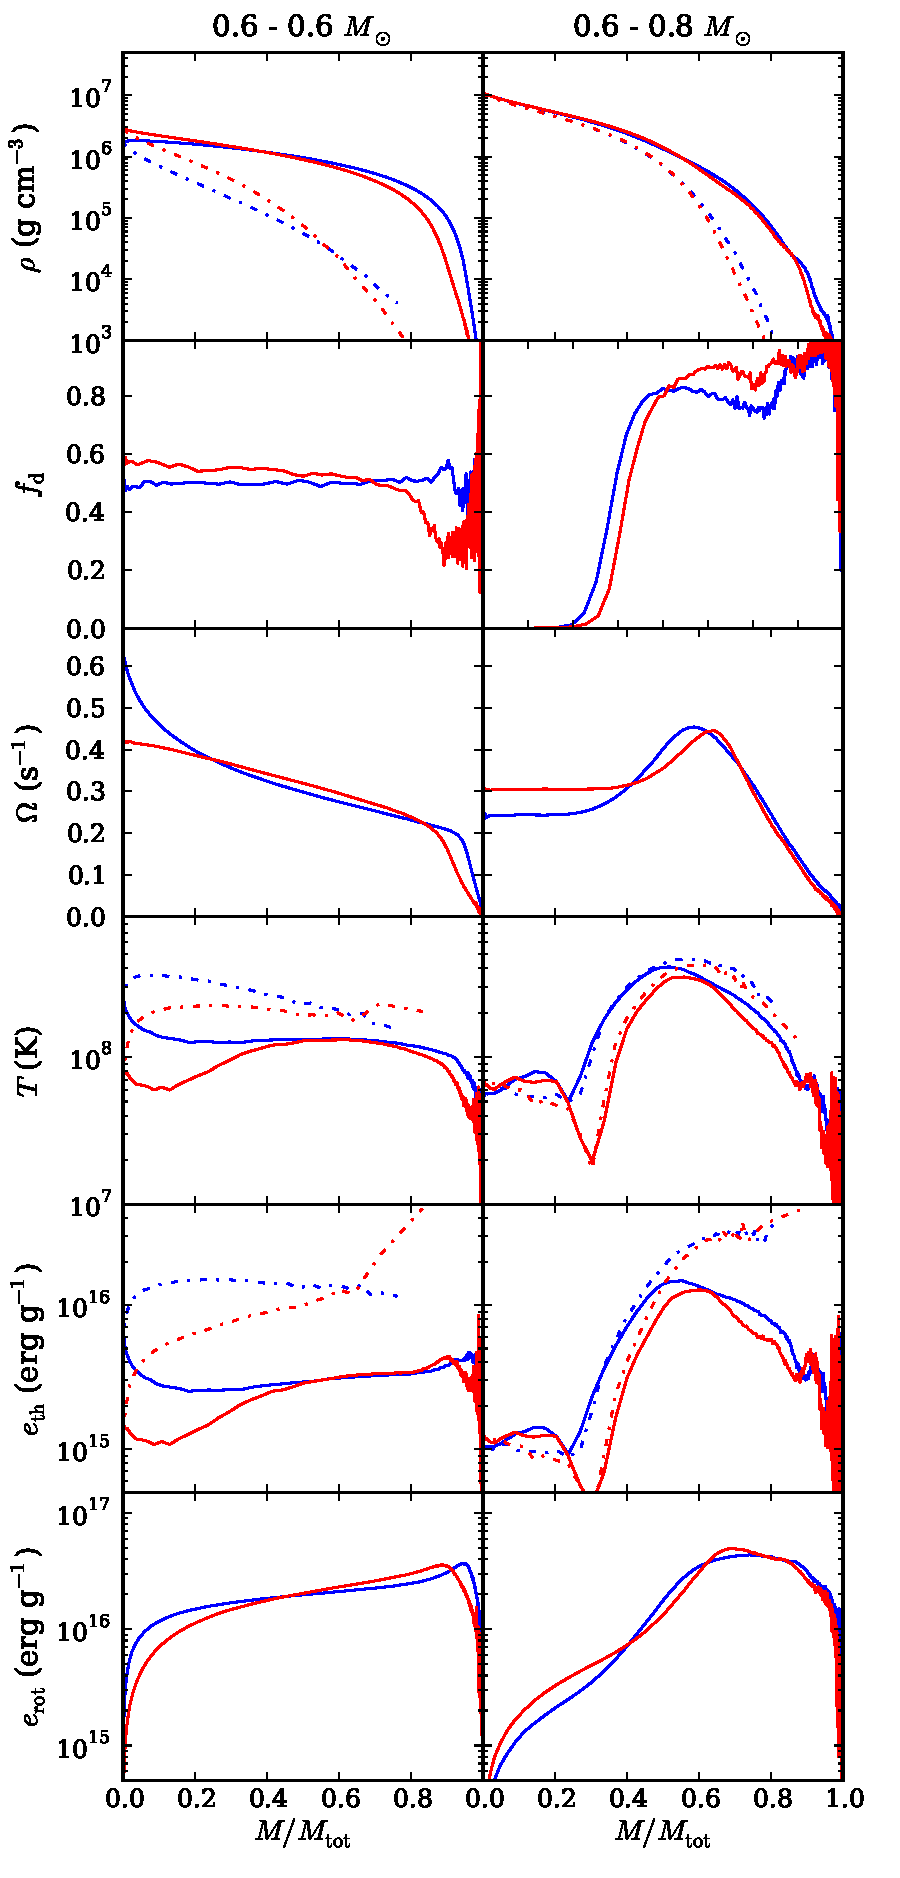
\includegraphics[angle=0,width=1.0\columnwidth]{synchcomp.pdf}
\caption{As Fig.~\ref{fig:compcomp}, but for 0.6 - 0.6 {\Msun} (left) and 0.6 - 0.8 {\Msun} (right) mergers, comparing our default, irrotational case (blue) with that assuming synchronous rotation (red).}
\label{fig:synchcomp}
\end{figure}

In our simulations, the WDs have zero spin, i.e., we assume that tidal dissipation is too weak to synchronize their rotation.  Whether or not this is correct is currently unknown, but to see what the effect could be, we ran simulations assuming synchronized rotation for 0.6 - 0.6\,\Msun\ and 0.6 - 0.8\,\Msun\ binaries (see Fig.~\ref{fig:synchcomp}).  We used approximate initial conditions for these systems, identical to those of Sec. \ref{ssec:initcond} except that the stars rotate at the orbital angular frequency.

As in Sec.~\ref{ssec:varyingazero}, our unsynchronized runs are from our parameter space study, and use 6 orbits as their completion criterion, while our synchronized runs use 2.5\% non-axisymmetry, and a requirement for the density to be highest at the remnant's center.  Completion occurred at 407 s ($\sim$8.5 orbits) for the synchronized 0.6 - 0.6 {\Msun} simulation, and 314 s ($\sim$6.5) orbits for the synchronized 0.6 - 0.8 {\Msun}.

The asynchronous and synchronous mergers differ mostly in the amount of heating and spin-up.  This has two causes.  First, for the synchronized binary, the total amount of angular momentum is about 10\% larger, and high angular momentum material has more difficulty penetrating the accretor, as is evident in the 0.6 - 0.8 {\Msun} mixing profile (because of the larger amount of angular momentum, the mergers also take about 1.5 orbits longer to achieve 2.5\% non-axisymmetry).  Second, in a synchronized binary, the donor and accretor have much less differential rotation with respect to each other, leading to much less spin-up and heating.

Both effects are largest for the equal-mass case.  In particular, in a synchronized, equal-mass binary contact can occur without any friction, while in an unsynchronized one it involves shocks at the full orbital velocity.  In consequence, for the synchronized case, rotational support is weaker in the center and stronger in the outskirts, causing the central density of our 0.6 - 0.6 {\Msun} remnant to increase by $\sim70$\% and the disk mass to increase by a factor of 2.  Furthermore, while for the non-synchronized case, the maximum temperature along the equatorial plane was found in the center, for the synchronized case it is found in the outskirts, and is more than a factor two lower ($1.3\times10^8\,$K instead of $2.9\times10^8\,$K).  The hotspots on the rotational axis also have much reduced temperature, $2.3\times 10^8$\,K instead of $3.6 \times 10^8$\,K.  
%This overall lowering of temperature, and change in the location of equatorial maximum temperature, are due to the initial accretion streams and dense torus produced during equal mass mergers experiencing much less heating in the synchronous case.

For the dissimilar-mass merger, the effects of synchronization are less dramatic: the accretor still spins up substantially, and rotational and thermal energy are deposited in roughly the same way.  The main difference is that the synchronized case has slightly less mixing, causing a drop in total thermal energy and maximum temperature (from $4.1\times10^8$ K to $3.5\times10^8$ K on the equatorial plane, and from $4.6\times10^8$ K to $4.3\times10^8$ K on the rotational axis).

%The main difference between the asynchronous and synchronous cases is the total amount of angular momentum in the system: $L_{\rm tot}$ is about 10\% larger in the synchronous case compared to the asynchronous case.  This does not necessarily translate to greater angular momentum in the remnant, $L_{\rm rem}$, because high angular momentum material has difficult accreting.  This is seen in the masses of the remnants where the masses of the synchronous cases is smaller than that of the asynchronous cases, while the masses of the disk is larger (at least in the 0.6-0.6 case).  The reduced angular momentum of the remnants translates into a lower value of $\Omega_{\rm max}$ and $E_{\rm rot,rem}$ in the synchronous case, while the mass coordinate of $\Omega_{\rm max}$ seems unaffected.  The smaller masses of the remnants also appears to translate to a lowering of the maximum temperature in the synchronous cases and in moving its mass coordinate in the case of the 0.8-0.6 merger.

\subsection{Running the Simulation Longer}
\label{ssec:runninglonger}

\begin{figure}
\centering
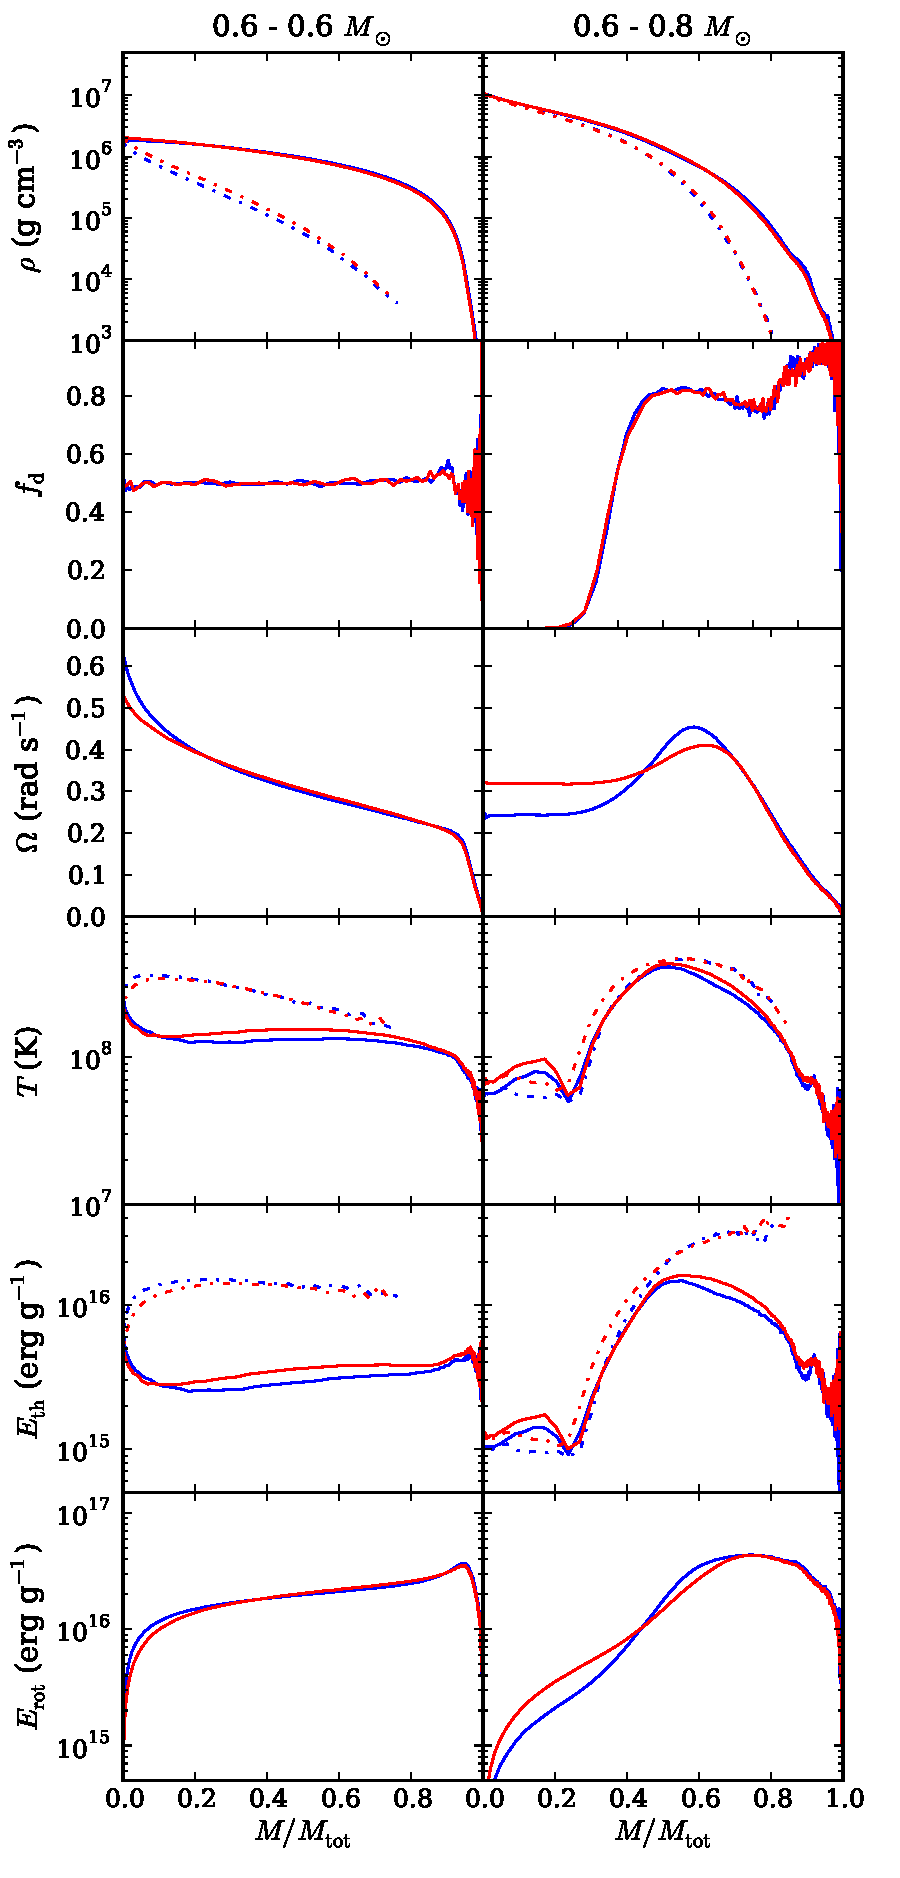
\includegraphics[angle=0,width=1.0\columnwidth]{timecomp.pdf}
\caption{As Fig.~\ref{fig:compcomp}, but for 0.6 - 0.6 {\Msun} (left) and 0.6 - 0.8 {\Msun} (right) mergers, comparing properties for our default simulation time of 6 initial orbital periods (blue) with those obtained after 8 orbital periods (red).}
\label{fig:timecomp}
\end{figure}

We considered our mergers completed after 6 orbits, since in that time they on average had reached our convergence criterion of 2.5\% non-axisymmetry (see Sec.~\ref{ssec:mergercomplete}).  To test the robustness of our results, we also determined properties attained after 8 orbits.  In Fig.~\ref{fig:timecomp}, we compare the 6 and 8 orbit results for 0.6 - 0.6\,\Msun\ and 0.6 - 0.8\,\Msun\ binaries.

We find our mergers show little evolution between 6 and 8 orbits, with the largest changes seen for the angular velocity profiles.  For the 0.6 - 0.8 {\Msun} merger, the rigidly rotating core sped up and the off-center peak decreased in height and moved out, while for the 0.6 - 0.6 {\Msun} merger, the center spun down and the rotational profile became flatter.  In the dissimilar-mass merger, \Tmax\ and \rhoTmax\ changed by $\lesssim\!5$\% and the density and temperature structures nearly overlap, while in the equal-mass merger \Tmax\ and \rhoTmax\ changed by $\sim\!20$\% ($2.9$ to $2.3\times10^8\,$K and $1.7$ to $2.0\times10^6\,\gcc$), reflecting an increase in central density and a shifting of the temperature profile, with temperature decreasing in the center but increasing elsewhere.  The evolution of all properties is consistent with viscous evolution -- expected to follow the merger proper -- with the core driven into rigid rotation, and angular momentum transferred outward to the disk.  In the dissimilar-mass merger, the net effect is spin-up of the core and spin-down of the envelope, while in the equal-mass case it is the reverse.  Of course, in the process, rotational energy is turned into thermal energy, heating the remnants.

One curious aspect for equal-mass mergers is the evolution of the off-center hot spots (Fig.~\ref{fig:mergersampling2}).  Over time, these broaden parallel to the equatorial plane, yet become narrower along the rotational axis.  As a result, the hourglass shape is lost, and the center of the remnant stops being one of the hottest point in the system.  After 8 orbits, the system resembles more closely what we find for typical similar-mass mergers, which have more pancake-shaped hot spots flanking a colder, denser region on the equatorial plane.

%Comparing more broadly the 6 and 8-orbit results, we find changes at the $\lesssim\!5$\% level.  Exceptions include the central temperature, which changes by 20\% (for unequal masses this is due to a combination of spurious heating and heating due to spin-up, while for equal mass mergers the reason is detailed above), \Tmax\ by 7\%, \rhoTmax\ by 9\%, and \Omegamax\ by 9\%.  The density and enclosed mass of the hottest point along the $z$-axis can also shift substantially, partly due to the evolution of the off-center hotspot in equal mass mergers, and partly due to noise in the tenuous envelope.  With viscous evolution towards rigid rotation, we also see changes of up to 10\% in the core-envelope and disk rotational energy and angular momentum.

%When comparing the entire set of merger remants found using 2.5\% non-axisymmetry to those found using 1\%, the central density has increased $\sim$15\% for equal mass mergers (negligibly for unequal mass mergers), while the central temperature has increased $\sim$9\% for unequal mass mergers (though this may be due to spurious heating; see Sec. \ref{ssec:spheat}).  The maximum temperature has not changed significantly, but {\rhoTmax} has increased by $\sim$13\% for all mergers.  The disk has decreased by $\sim$5\% for unequal mass mergers (more than $\sim$10\% for highly unequal mass mergers), and increased by $\sim3$\% for equal mass mergers.  For unequal mass mergers the central $\Omega$ has increased by an average of $\sim$16\% with a corresponding drop in {\Omegamax} by $\sim$4\%, while for equal mass mergers the central $\Omega$ has dropped by $\sim$10\%.  All these trends are consistent with those seen in Fig. \ref{fig:timecomp}, indicating the figure's curves as being generalizable to all equal and non-equal mass mergers.  \textbf{CUT THIS PARAGRAPH?}

Comparing more broadly the 6 and 8-orbit results, we find changes at the $\sim\!5$\% level.  The trends presented in Sec.~\ref{ssec:mergertrends} continue to hold to within $\sim\!10$\% except for \hxy\ (which becomes $\hxy/h_{\rm a} = 0.98 + 0.74q_\rho^2~(\pm0.07)$), the fraction of disk energy in degeneracy energy ($E_\mathrm{deg,disk}/E_\mathrm{I,disk} = 0.07~(\pm0.02)$), mass enclosed within the radius of maximum temperature ($\MencTmax/\Ma = 1-0.21q_\rho~(\pm 0.01)$), maximum rotational frequency ($\Omegamax/\Omegaorb = 3.4~(\pm0.5)$) and the widths of the regions in which thermal and rotational energy are deposited ($\MEthermthick/\Ma = 0.13 + 0.87q_\rho ~(\pm0.03)$; $\MErotthick/\Ma = 0.15 + 0.70q_\rho ~(\pm0.02)$).  Changes to these trends are consistent with the viscous evolution described above: the remnant is beginning to spin down, lose its rotational support, and energy is being redistributed.

\subsection{Viscosity Prescription}
\label{ssec:viscprescrip}

The addition of artificial viscosity is required in SPH to accurately capture shocks, but no consensus exists on how best to implement it.  We ran two additional simulations of a 0.6 - 0.8\,\Msun\ merger to check the robustness of our results with respect to changes in the viscosity, one with small and one with large artificial viscosity (fixed $(\alpha,\beta)=(0.05,0.1)$ and $(1,2)$, respectively).  As before, these additional runs use 2.5\% non-axisymmetry and a requirement for the density to be highest at the remnant's center as their completion criteria, and the low viscosity run completed at 198 s while the high completed at 242 s.  Here, we expect that low values of $\alpha$ will lead to large particle noise and inaccurate shock capturing, while high values result in large viscous heating and rapid loss of differential rotation.  Our results confirm this (Fig.~\ref{fig:viscnumcomp}): the simulation with low artificial viscosity leads to a remnant with stronger differential rotation, with the disk carrying 34\% more rotational energy (and the remnant 33\% less) than in the standard variable $\alpha$ simulation.  Lower viscosity also leads to greater mixing of donor and accretor material, reflecting the stronger diffusion associated with the larger particle noise inherent to low viscosity.

Aside from the mixing and spin-up, the results for the three different viscosity prescriptions do not differ greatly.  While one might have expected greater dissipation of rotational into thermal energy for higher viscosity, the maximum temperatures and rotation rates vary by $\lesssim\!10$\%, and the thermal and rotational profiles are quite similar.  The density profiles are virtually identical except near the outer parts, where the low viscosity simulation leaves matter with greater rotational support.  

%CZ: This is wrong, according to James - his e-mails indicate he does not think spurious heating goes up with lower viscosity.  "The largest and initially most curious difference between the three simulations is that of central temperature, where for high viscosity we find a low central temperature and for low viscosity a high one.  This reflects the changes in spurious heating due to particle noise, which we discuss next."

%MHvK: keeping this sentence about equal-mass mergers is an invitation for a referee to ask why we do not test that...
%Both the density and temperature curves, however, might change more for equal mass mergers, since mixing of the entire remnant is a more important contributor to the final remnant structure in those cases.

%To determine how much our viscosity prescription can affect the outcome of our merger, we ran a 0.6 - 0.8 {\Msun} merger with the viscosity artificially low ($\alpha\,=\,0.05$, $\beta\,=\,0.1$) and artificially high ($\alpha\,=\,1.0$, $\beta\,=\,2.0$).  The former should be unable to properly capture any shocks that arise during the initial merger, while the latter will produce unphysically large viscous heating and reduction of differential rotation following the merger.  The results reflect this (Fig. \ref{fig:viscnumcomp}): mixing in the low-viscosity run is more thorough than in the high-viscosity one (where friction stops the donor from penetrating into the accretor).  The spin-up of the remnant core is much greater in the high-viscosity run, and the temperature peak is also higher and more narrow (due to lack of donor penetration).  Since most of the support of the remnant against gravity is due to degeneracy pressure, the density curves do not differ significantly.  Curiously, while most of the variable $\alpha$ curves resemble their low viscosity counterparts, the rotation and rotational energy curves more closely match the high viscosity ones.  This is perhaps because the angular velocity curve structure is set during the first few seconds of merger, just after the donor is disrupted, or perhaps during the latter stages of the merger $\alpha$ is still high in the $\Omega$ peak.  \textbf{I'M MAKING MOVIES TO SEE WHICH IS TRUE.}

%Many of the merger remnant properties change by more than 20\% between the different viscosity runs, including the number of orbits required to complete merger ($\sim25$\%), the central and maximum temperature ($\sim30$\% for {\Tc} and $\sim25$\% for {\Tmax}), {\MencTmax} ($\sim25$\%), and the disk energies ($\sim20$\% on average).  Density values unassociated with {\Tmax} and {\Omegamax} remain largely unchanged (ex. {\rhoc} changes by 2\% from variable $\alpha$ for both high and low viscosity).  Comparative runs for our entire parameter space have not been completed, so it is not certain if the remnant trends will still scale as they do in Sec. \ref{ssec:mergertrends}.

\begin{figure}
\centering
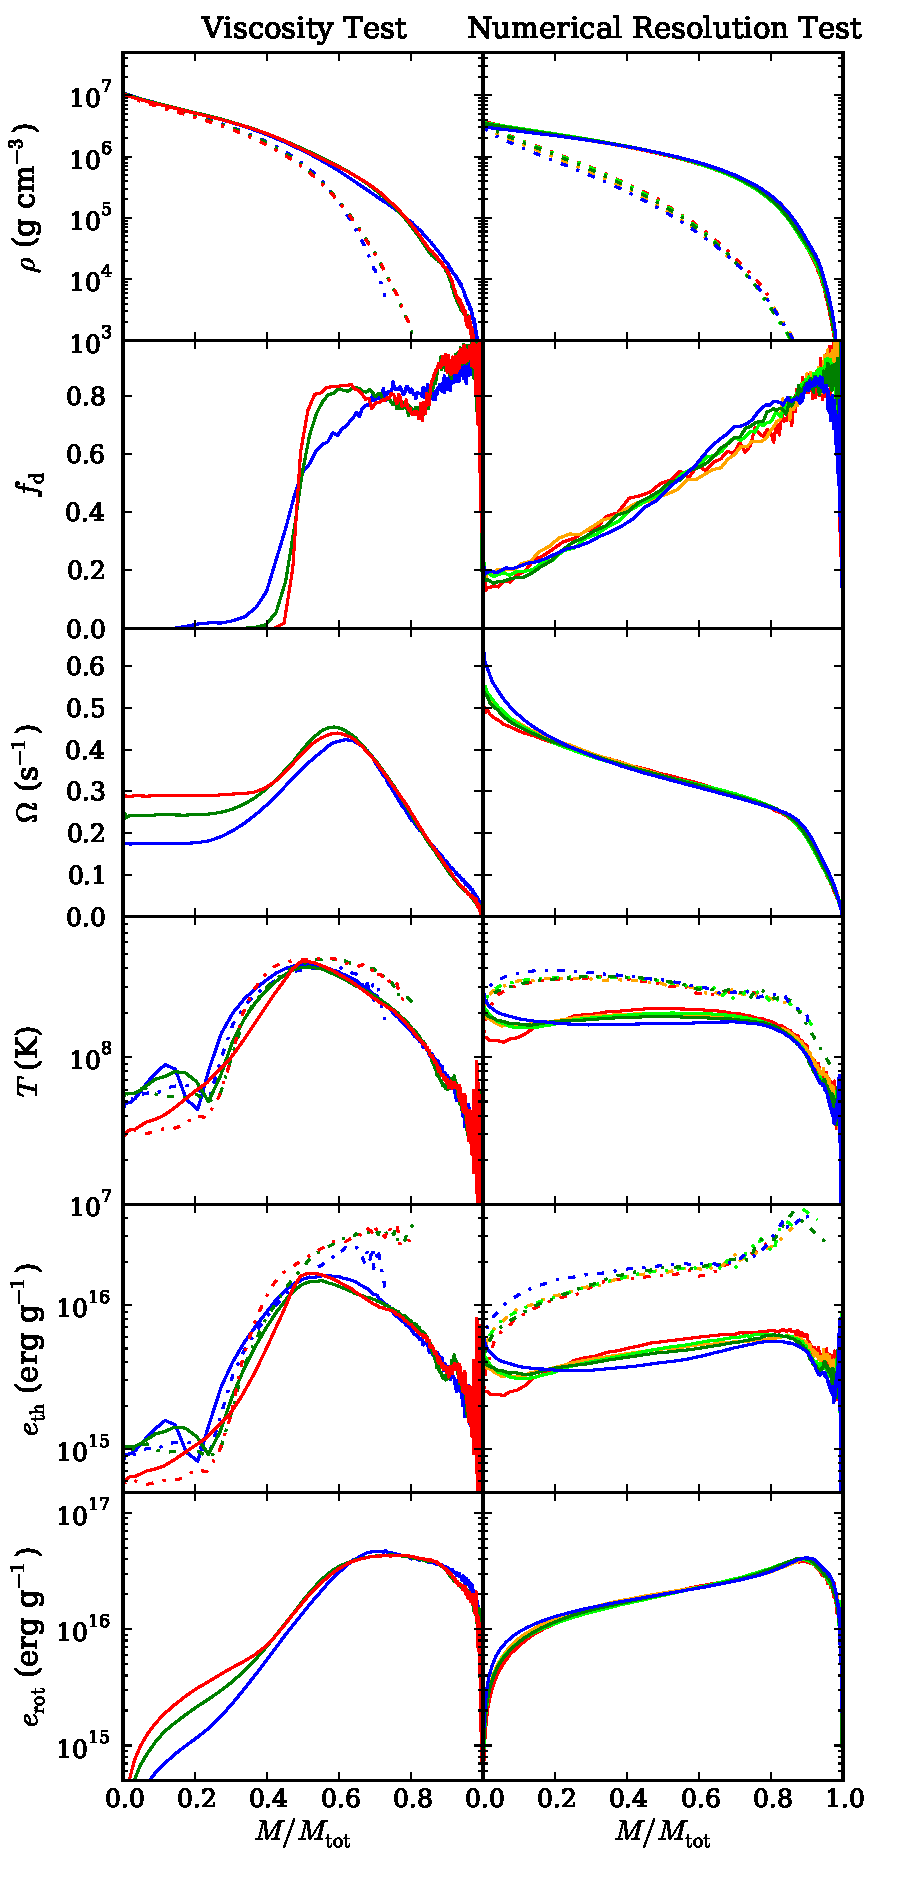
\includegraphics[angle=0,width=1.0\columnwidth]{viscnumcomp.pdf}
\caption{As Fig.~\ref{fig:compcomp}, but comparing simulations of a 0.6 - 0.8\,\Msun\ merger with different viscosity prescriptions (left) and simulations of a 0.625 - 0.65\,\Msun\ merger with different numbers of particles (right).  For the viscosity, we compare fixed low viscosity ($\alpha=0.05$, $\beta=0.1$; blue), standard variable viscosity (green), and fixed high viscosity ($\alpha=1.0$, $\beta=2.0$; red).  For particle numbers, we show simulations at one quarter (red), half (orange), and double (blue) the default number of particles, as well as the default simulation (lime) and a rerun of the default simulation (green) to determine the effect of order-of-execution differences, round-off errors and other such numerical effects.}
\label{fig:viscnumcomp}
\end{figure}

\subsection{Spurious Heating}
\label{ssec:spheat}

As discussed in Sec.~\ref{ssec:sphcode} and throughout Sec.~\ref{sec:results}, noise combined with a pressure floor in the equation of state lead to small increases in internal energy.  While this energy has a negligible effect on most remnant properties, in the most degenerate regions of the remnant it can cause significant temperature increases.  Here, we discuss the extent to which spurious heating affects our results.

As a comparison for the spurious heating seen in some of the simulations, we relaxed a 0.8\,\Msun\ isolated white dwarf for $489\,$s longer than the standard 81\,s we used for relaxing single stars.  While the total energy of the WD (potential, degeneracy and thermal energy combined) increased by $\sim\!1$\% of the original total energy over the additional period of time, the change in thermal energy was enough to raise the central WD temperature from $1.2\times 10^7$ K (increased from $5\times 10^6$ K due to particle noise) to $1.2\times 10^8\,$K.  In Fig.~\ref{fig:heating}, we compare the thermal energy profile of this isolated 0.8 {\Msun} WD with those of a 0.4 - 0.8\,\Msun\ and a 0.7 - 0.8\,\Msun\ merger, with the times for the isolated WD taken at 489 and 224\,s (the mergers' respective completion times) longer than the standard 81\,s.  The total thermal energy generated in the WD at an additional 489\,s is $\sim$10\% of the thermal energy generated in a 0.4 - 0.8\,\Msun\ merger.\footnote{A $\sim$10\% increase in thermal energy corresponds to $\sim\!1$\% increase in the overall energy of the 0.4 - 0.8\,\Msun\ remnant, somewhat larger than the typical $\sim\!0.3$\% level at which Gasoline conserves total energy in our simulations.  We find that similar-mass simulations tend to lose total energy at the 0.05\% level, while some of the low {\qrho} mergers gain more than 1\% in total energy due to spurious heating.}  Indeed, given how well the specific thermal energy profiles match in the interior, it is clear that spurious heating dominates there.  

Spurious heating is much less important for the 0.7 - 0.8\,\Msun\ merger, since its core has mixed to much greater extent and less time was needed for the merger to complete.  The total thermal energy generated in the isolated WD at 224\,s is only $\sim\!3$\% of the thermal energy generated during merger, and even at the very center spurious heating contributes $\sim\!35$\% (rather than nearly all) of the thermal energy.  As a result, the central temperature of the merger, $1.4 \times 10^8\,$K, is substantially higher than that of the isolated WD, $7.8 \times 10^7\,$K.  It is important to note this comparison overestimates spurious heating, since the isolated WD will have had many more particles that dip below the Fermi energy than the much hotter merger remnant core. 

%MHvK: bit unclear about point of this, so shortened
%We note that post merger heating of remnant cores is at least partly also due to spin-up of the core, and that in equal mass mergers there is little in terms of thermal evolution of the core to suggest spurious heating is actually occurring.  We therefore do not know for certain if spurious heating results from a lone, inert WD can directly be applied to our merger remnants.  Nevertheless, when the center of a merger remnant has not been heated by the merger to temperatures above $10^8$ K, we believe spurious heating provides a substantial contribution to the total energy of the core.  This renders core temperature would be higher than expected for these systems.  The effect should not be significant for high density material with $T\gtrsim3\times10^8$ K where spurious heating is small compared to the thermal energy, and for low-density ($\rho \lesssim10^5$ {\gcc}) material where the material is non-degenerate.    

Overall, we conclude that spurious heating is present, but is recognized fairly easily and does not influence our conclusions.  In particular, its effects on remnants should be small in both high-density regions with $T\gtrsim3\times10^8$\,K and in lower-density $\lesssim\!10^6\,\gcc$ regions.  Other simulations may suffer from spurious heating as well.  In this respect, it is intriguing that our equatorial temperature curves for a 0.6 - 0.8\,\Msun\ merger are a good match those of \citetalias{loreig09}, even in the center (Fig.~\ref{fig:compwithloreig}; Sec.~\ref{ssec:compwithloreig}).

%The spurious heating may be minimized by an appropriate choice of the viscosity prescription.  For instance, a larger viscosity would reduce particle noise, which in turn would reduce spurious heating.  However, a large viscosity would also increase dissipation of differential rotation.  Other simulations may suffer from spurious heating as well.  In this respect, it is intriguing that our equatorial temperature curves for a 0.6 - 0.8\,\Msun\ merger are a good match those of \citetalias{loreig09}, even in the center (Fig.~\ref{fig:compwithloreig}; Sec.~\ref{ssec:compwithloreig}).

\begin{figure}
\centering
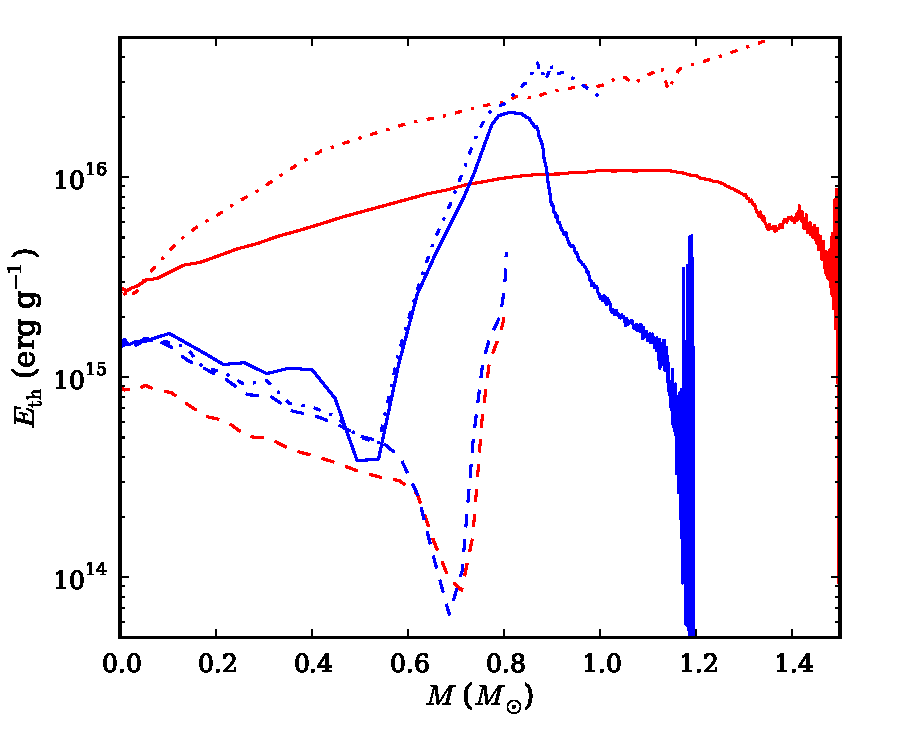
\includegraphics[angle=0,width=1.0\columnwidth]{heatingTEC.pdf}
\caption{Specific thermal energy as a function of enclosed mass for a 0.4 - 0.8 {\Msun} (blue) and a 0.7 - 0.8 {\Msun} merger (red), shown both along the equatorial plane (solid curves) and along the rotational axis (dot-dashed).  Also shown are the (spherical) profiles found for an isolated 0.8\,\Msun\ white dwarf (dashed) simulated using the same parameters, and for the same completion times (six initial orbital periods, equivalent to 489 s and 224 s).  Spurious heating is estimated to be responsible for nearly all the thermal energy in the core of the 0.4 - 0.8\,\Msun\ remnant, and for about one third in the core of the 0.7 - 0.8\,\Msun\ remnant.  It is not important in regions heated by interaction.  (The ``hook'' in the outer layers of the white dwarf profile reflects the high initial temperature chosen; in a merger, this is erased by the interaction.)}
\label{fig:heating}
\end{figure}

\subsection{Resolution}
\label{ssec:restest}

%\begin{figure}
%\centering
%\includegraphics[angle=0,width=0.35\columnwidth]{numcomp.pdf}
%\caption{Comparison of 0.625 - 0.65 {\Msun} mergers performed at different numerical resolutions.  Red indicates 63,736 (1 particle = $4\times10^{28}$ g), orange 127,525 ($2\times10^{28}$ g), lime and green 255,035 ($1\times10^{28}$ g) and blue 510,047 particles ($5\times10^{27}$ g).  The 255,035 particle run was completed twice using identical initial conditions to determine the effect of random errors on our simulation.  Completion time was set to 270 s (6 orbits of the 255,035 run) for all simulations.  See Fig. \ref{fig:constacc}'s caption for details on each subplot.}
%\label{fig:numcomp}
%\end{figure}

To determine whether or not the numerical resolution matters for our results, we ran three additional simulations of a 0.625 - 0.65 {\Msun} merger, with roughly a quarter, half, and double the number of particles (63,736, 127,525 and 510,047, respectively), corresponding to 0.63, 0.79 and 1.26 times the SPH smoothing length (resolution) we normally use.  We also ran a second simulation with the same number of particles (255,035 particles).  Here, we chose 0.625 - 0.65\,\Msun\ to see if numerical resolution has any effect on whether a merger is ``similar-mass''.  All simulations were considered complete at 6 orbits of the initial binary, though we also checked the 2.5\% non-axisymmetry convergence times.

From Fig.~\ref{fig:viscnumcomp}, one sees that the two runs using the same number of particles -- and identical initial conditions and the same version of Gasoline -- still give slightly different results.  This is due to the inherent non-linear nature of fluid dynamics, coupled with small, random perturbations, e.g., from differences in the order of force addition in parallel processing, round-off errors and slight inconsistencies in converting thermal energy to temperature.  Overall, merger remnant properties change by $\sim3.5$\% between the two runs.  The most prominent differences are seen in properties determined from low numbers of particles, such as {\Tc} (varies by $\sim10$\%), and those involving finding maxima of temperature plateaus, such as \zrhoTmax\ (40\%) and $\rho(T^\mathrm{cv}_\mathrm{max})$ (a factor of 3 -- in one case convection shifts the temperature maximum off-center).

%The most prominent differences are seen in the temperature and thermal energy profiles: maximum thermal energy differs by 4\% between the two simulations.  

The differences for different resolutions are larger.  While to first order, the equatorial density and mixing profiles are very similar, there is a systematic $\sim\!20$\% drop in the equatorial density -- $\sim\!25$\% in the rotational axis density -- near the center of the remnant with increasing numerical resolution (top right panel of Fig.~\ref{fig:viscnumcomp}).  The angular velocity and rotational energy profiles are again very similar, except in the central regions, where there is a $\sim\!20$\% increase in \Omegamax.  For the temperature the effects are larger: with higher resolutions, most of the equatorial plane is colder, with a $\sim20\!$\% drop in the value of the temperature plateau near $M/M_\mrm{tot}\,=\,0.5$.  The temperatures along the rotational axis, however, increase with increasing resolution, by $\sim\!10$\% across the range of resolutions, as does the upturn in equatorial temperature near the center of the remnant, by $\sim\!50$\% ($\sim\!30$\% if we do not include the lowest resolution run).  The latter effects are due to increasing prominence of the off-center hotspots at higher resolutions, which also tend to look more hourglass-shaped.  Indeed, for our lowest resolution, the densest material in the two stars remains relatively cold throughout the entire merger, resembling the synchronized systems described in Sec.~\ref{ssec:synchronization}.  Finally, we find that if we do not consider the lowest resolution run, the disk half-mass radius varies by 4\%, angular velocity at the half-mass radius varies by 4\%, and the core-envelope mass changes by 3\%.  This is similar to the results of the resolution tests of \cite{rask+12}.

%\emph{rask+12 say this is disk mass, but they labeled their figure with Mc, and disks aren't a solar mass}

The 2.5\% non-axisymmetry convergence times for the half and double-particle number runs are within 14 s of the 275 s non-axisymmetry convergence time of the default run, a small difference that implies a negligible amount of post-merger evolution.  Only the quarter-particle number run deviated substantially, converging 57 s earlier.  This may simply reflect the smaller number of particles in the disk, where the system is most asymmetric.

We stress that even though the order-of-magnitude change in particle number (factor of two change in resolution) generates 10 -- 30\% variations in some remnant properties, the overall shapes of the profiles in Fig.~\ref{fig:viscnumcomp} are very similar.  In particular, the merger remnant does not look more or less ``similar-mass'' (except, arguably, the temperature curve at the lowest resolution).  Exact values of properties, therefore, will vary depending on resolution (and will vary on similar or larger levels if initial conditions like \azero\ are changed), but the overall picture of the merger and trends should be more robust.

%We thus conclude that our trends should be robust.

% Since the general conclusions of this work are not dependent on exact values of merger remnant properties, numerical resolution should not drastically change our conclusions.

\section{Comparison With Others}
\label{sec:compwithothers}

%{\bf note that Loren-Aug is much more viscous than our results}

\subsection{Comparison With \cite{loreig09}}
\label{ssec:compwithloreig}

\citeal{loreig09} simulated a number of WD mergers, and gave detailed temperature, surface density, and rotational frequency curves for three.   In Fig.~\ref{fig:compwithloreig}, we compare their results (from their Figs. 3 and 4) with ours for two of these, 0.6 - 0.6\,\Msun\ and 0.6 - 0.8\,\Msun\ (the third was a 0.4 - 0.8\,\Msun\ He - CO WD merger, whose temperature profile cannot be compared directly).  We note that they used different initial conditions, starting their systems with an orbital separation too large for mass transfer to begin, and then slowly reducing the separation until it does.  This point defines their $t = 0$ and the start of the merger simulation proper.  Given this different setup, their merger completion times cannot be compared directly to ours.  In their simulations, however, coalescence (the final consolidation of the two WDs into one) also occurs after just about one orbit, so the differences should not be too large.  To give a sense of the effect of different completion criteria, we compare their results both with our standard results, taken after 6 orbits, and our results taken at their merger completion times.

For both mergers, the surface density curves are similar, although in their 0.6 - 0.6\,\Msun\ merger, the central peak is $\sim\!30$\% higher ($\sim\!10$\% if we use their completion time of 514\,s).  For the 0.6 - 0.8\,\Msun\ merger, the temperature profiles are also very similar, with maxima\footnote{Maximum temperatures given in Table 1 of \citeal{loreig09} refer to hot spots in their simulations, and are about a factor of 2 higher than the hottest points on their temperature curves.  As we have not done hot-spot finding, we cannot compare with those values.} differing by only $\sim$10 - 15\%, and having nearly identical shapes.  Larger differences are seen for the 0.6 - 0.8\,\Msun\ rotational frequency profile, where the angular velocity peaks further out and at lower value ($\sim\!0.3\,\psec$ compared to our $0.45\psec$ -- or $0.50\,\psec$ using their completion time of 164 s).  Indeed, our entire remnant is more spun-up than theirs.  

For the 0.6 - 0.6\,\Msun\ merger, \citeal{loreig09} have a plateau in their angular frequency profile, with $\Omegamax\simeq0.25\,\psec$, while our profile is much more peaked and reaches a much higher frequency, of $0.60\,\psec$.  By their completion time, our rotation curve is not as sharply peaked, but still reaches $0.44\,\psec$.  The temperature profiles are also much less similar: our maximum temperature in the equatorial plane is a factor of 2 lower than theirs (factor of 3.3 at their completion time), and even our maximum temperature along the rotational axis is a factor 1.6 lower (factor 1.9 at their completion time).  

Finally, we can compare how mass is distributed.  In both our simulations and those of \citeal{loreig09}, negligible mass is lost, so only the distribution between disk and core-envelope matters.  For our 0.4 - 0.8\,\Msun, 0.6 - 0.6\,\Msun, and 0.6 - 0.8\,\Msun\ simulations, we infer disk masses  of 0.31, 0.10, and 0.40\,\Msun, respectively, which are reasonably close to the 0.28, 0.10, and 0.30\,\Msun, respectively, listed by \citeal{loreig09} (their Table~1), especially considering that we likely use a different definition of what is ``disk''.

Overall, the primary differences between our simulations appear to be the amount of spin-up and heating of the equal-mass merger.  We believe it is unlikely that this reflects differences in initial conditions: we found much smaller changes in the angular velocity profile with increasing {\azero} (see Fig.~\ref{fig:distcomp}), and in the simulation of \citeal{loreig09} the stars still seem to be quite close to spherically symmetric at the start and disrupt quickly (their Fig.~1), even though they were more properly relaxed.  Instead, we believe the more likely explanation is that the viscosity prescription of \citeal{loreig09}, based on Riemann solvers, yields larger effective viscosity.  This would explain both the reduction in angular velocity and increase in temperature (since viscous evolution converts rotational into thermal energy), as well as the fact that similar-mass mergers are affected more (they mix more, and \citeal{loreig09} ran their equal-mass merger for a very long time).  If we ran our simulations longer and thus included further viscous evolution, the similarity with their simulations would likely be closer.

\begin{figure}
\centering
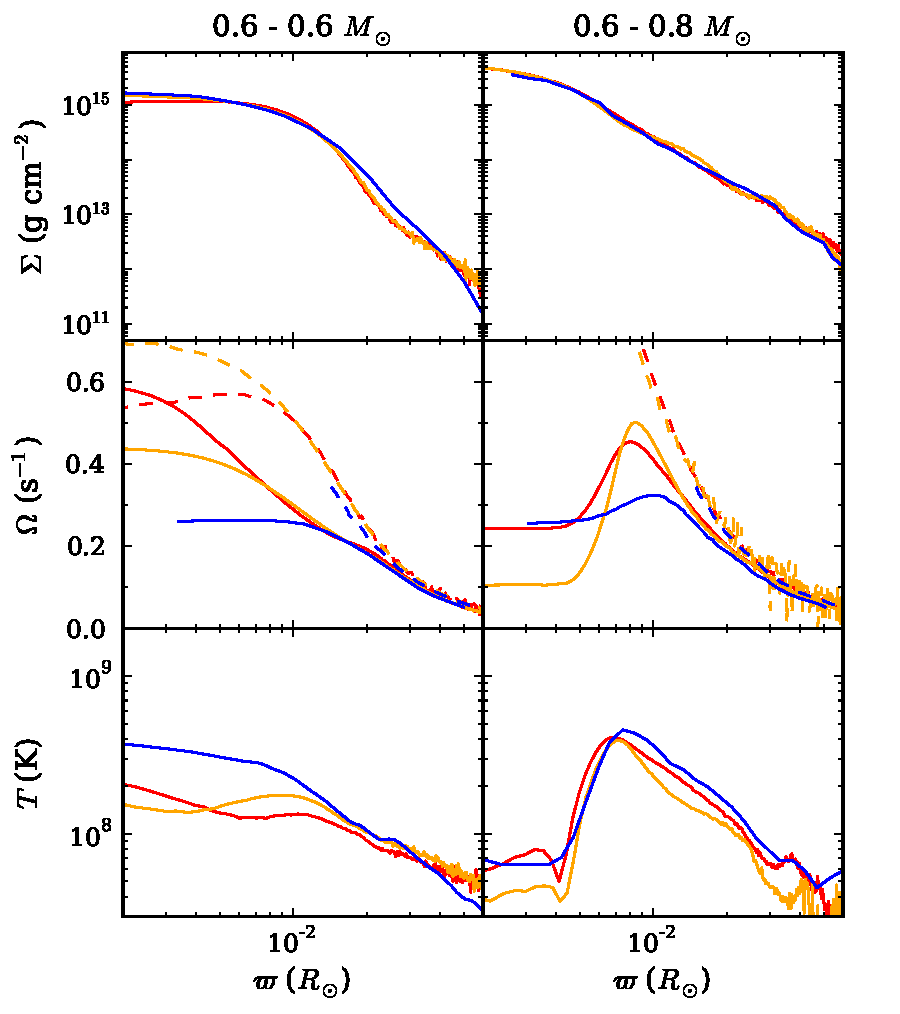
\includegraphics[angle=0,width=1.0\columnwidth]{compwithloreig.pdf}
\caption{Comparison of our results with those of \citetalias{loreig09}, for a 0.6 - 0.6\,\Msun\ (left) and a 0.6 - 0.8\,\Msun\ (right) merger.  Shown are surface density, remnant (solid) and Keplerian (dashed) angular frequency, and temperature, with profiles from \citetalias{loreig09} in blue, and our equivalent ones in red and orange.  Here, the former are for our default completion time of 6 initial orbital periods and the latter for their completion times (514 s or 10.9 orbital periods for the 0.6 - 0.6\,\Msun\ merger, and 164 s or 3.4 orbits for the 0.6 - 0.8\,\Msun\ merger).}
\label{fig:compwithloreig}
\end{figure}

%The differences between our results and those of \citetalias{loreig09} are not because of our 2.5\% non-axisymmetry merger completion criterion - Fig. \ref{fig:compwithloreig} also shows curves from our simulations at \citeal{loreig09}'s stated completion times, and these curves look a more similar to our results than \citeal{loreig09}'s.  Our differences could be due to differences in the artificial viscosity implementation, as we use the variable $\alpha$ scheme while \citetalias{loreig09} uses a method based on Riemann solvers.  They could also be due to initial condition setup.  \citeal{loreig09}'s binaries do not start close enough to each other to immediately prompt Roche Lobe overflow; instead, an artificial radial acceleration is used to slowly bring the two stars in until one begins to transfer mass to the other.

\subsection{Comparison with Others}
\label{ssec:compwithothers}

Simulations of WD mergers have also been presented by \citet{yoonpr07}, \citet{pakm+10,pakm+11,pakm+12}, \citet{dan+11,dan+12}, and \citet{rask+12}.  Unfortunately, comparison with those results is difficult, since, unlike \citeal{loreig09}, all these authors are sparse with quantitative details about their results.

%run Analyzer.py pt8pt9o.36000.ascii
%[massR,massM] = getmassr(gasr, gasmass, dR)
%[densoutputR_S, densoutputval_S] = getsphericaldensity(gasx, gasy, gasz, gasdens, dR)
%[TempoutputR_S, Tempoutputval_S] = gettemphelm(gasx, gasy, gasz, gastemp, gasdens, dR)
%plt.plot(massR*6.95508e9/1e9,massM/1.9891e33,'r-')
%plt.semilogy(densoutputR_S*6.95508e9/1e9,densoutputval_S)
%plt.semilogy(TempoutputR_S*6.95508e9/1e9,Tempoutputval_S)

An exception is the 0.81 - 0.9 {\Msun} merger simulated by \cite{dan+12}, shown in their Fig.~1.  While that simulation is for synchronized WDs, it is still particularly useful to compare with, since \citeauthor{dan+12} show results for both approximate and accurate initial conditions.  We find that their spherically enclosed mass profile is very similar to ours, with, e.g., $M=0.9\,\Msun$ at $4.5\times10^8\,$cm in both (though since spherically enclosed mass is a cumulative quantity, significant structural differences can remain hidden).  Our spherically averaged density profile looks most similar to the profile they found using approximate initial conditions.  Our central density, $1.9\times10^7\,\gcc$, is within $\sim\!10$\% of theirs, and the density profile remains similar up to $r \simeq 5 \times 10^8\,$cm ($\rho\simeq10^6\,\gcc$).  Beyond, their profile becomes shallower while ours continues to decline; at $r=10^9\,$cm, they find $\rho\simeq3\times10^5\,\gcc$, while we find $\rho\simeq10^5\,\gcc$.  This may be a consequence of the additional angular momentum associated with synchronized rotation.  With accurate initial conditions, a difference with our results is that the density profile becomes flat beyond $10^9\,$cm.  

Comparing temperature profiles, we roughly reproduce their spherically averaged one for approximate initial conditions, including the off-center peak -- their \Tmax\ is $\sim\!20\%$ lower (to be expected since their binary is synchronized; see Sec.~\ref{ssec:synchronization}), but is also located at $4\times10^8\,$cm (or $M_r\simeq0.9\,\Msun$).  However, our central temperature ($2.2\times10^8$ K) is an order of magnitude higher than theirs ($2\times10^7$ K) and at $r\gtrsim10^9\,$cm our temperatures are systematically hotter, perhaps a result of the much larger dissipation expected for non-rotating WDs.  With accurate initial conditions they found an even narrower temperature peak than the one with approximate conditions, which thus deviates even more from our curve.  This trend is similar to what we see when increasing \azero\ (Sec.~\ref{ssec:varyingazero}), so it seems likely we would reproduce their simulations more closely if we used the same initial conditions.

\subsection{The Importance of Accurate Initial Conditions}
%MHvK: I felt this could use its own subsection.

Many of the recent simulations \citep{dan+11,dan+12,rask+12} assume co-rotating WDs.  This assumption is numerically convenient, in that it is relatively straightforward to start the simulation in the physically correct state: since in the co-rotating frame there are no flow velocities, one can easily relax a simulated binary within an appropriate potential in the co-rotating frame, damping out any velocities resulting from an initial mismatch.  

As a result, it has been possible to study the onset of mass transfer in detail.  As first pointed out by \citet{dsou+06} from simulations using a grid code, the disruption of the donor is preceded by a rather long -- dozens of orbits -- phase of mass transfer.  Further simulations by \cite{dan+11,dan+12} showed that in this initial phase a significant fraction, $\sim10\%$ of the donor mass, is transferred.  As a result, e.g., the disk is substantially colder and more extended.  The remnant core seems more subtly affected, in that its appearance becomes ``more dissimilar'', reflecting that coalescence is between two WDs whose masses have become more disparate than they were initially.  As a consequence, e.g., even for similar-mass binaries, the hottest point of the merger is found to be well outside the center.  Indeed, \citet{rask+12} find that even for equal-mass binaries, the final outcome for more massive mergers is one where the core of one of the WDs is virtually undisturbed.

%(i.e. evolution following full disruption of the donor)

%MHvK: not sure if we should remove it, but in the end I felt it distracted from the discussion; I added just a short sentence in the section above
%If the primary differences between our simulations and those of \cite{dan+12} are an extended period of mass transfer and synchronization, we can use the results of Sec. \ref{ssec:varyingazero} and Sec. \ref{ssec:synchronization}.  We found above that synchronized mergers have colder cores and slightly narrower off-center temperature plateaus, and an extended period of mass transfer has a similar effect.  For equal mass mergers, synchronizing and an extended period of mass transfer also have the effect of slightly increasing the spherical density of material at larger distances from the remnant center.  This suggests that we would much more closely reproduce the results of \cite{dan+12} if we used synchronized, accurate ICs.

%Nevertheless, we can use these {\azero} tests as a poor proxy of what the effect might be.  They show a trend toward less mixing between the two WDs and more narrowly peaked off-center temperature and angular velocity curves with increasing {\azero}.  A larger {\azero} also results in the binary surviving for many more orbits before total disruption of the donor is achieved.  Moreover, since a small amount of mass transfer occurs during this period of time, perhaps enough mass is transferred to render an equal mass merger ``dissimilar-mass'' at coalescence.  It is therefore possible that increasing {\azero} for equal mass mergers would allow us to qualitatively reproduce the results of \cite{dan+11,dan+12} and \citet{rask+12}.

At present, it is not clear how important accurate initial conditions would be for asynchronous mergers.  Qualitatively, we expect the effects to be smaller than for synchronous mergers, for three reasons.  First, from the analytic study of \cite{lairs94}, in which tidal and rotational distortion are approximated by ellipsoids, co-rotating binaries always reach contact or Roche lobe overflow before becoming dynamically unstable, while irrotational binaries become dynamically unstable first.  While an exact treatment of the irrotational case found that, in fact, Roche contact preceded dynamical instability \citep{uryue98}, it suggests that WDs in irrotational binaries will disrupt much sooner.  Second, the simulations of \citeal{loreig09} use initial conditions that should be quite close to correct, yet their WDs disrupt quickly (see Sec. \ref{ssec:compwithloreig}).  Third, the two components are counterrotating in the rotating frame.  Hence, any mass transferred will hit the accretor with a larger relative velocity than would be the case for co-rotating WDs.  Indeed, in the limit of equal-mass WDs, very little would happen for co-rotating WDs when one reaches contact, while a strong shock would be expected for the irrotational case.  In general, one expects part of the shocked material to enter a high-entropy halo around the accretor.  For co-rotating WDs, \cite{dan+11} found that this halo helps remove angular momentum from the orbit, leading to a shorter start-up phase.  For the irrotational case, given the stronger expected shocks, the start-up phase would likely be reduced even further.  On the other hand, we saw in Sec. \ref{ssec:varyingazero} that remnant properties are sensitive to changes in angular momentum content through changes in \azero.  Simulating more realistically the onset of mass transfer through accurate initial conditions will likely change \azero.

Ideally, one would still simulate the initial mass transfer phase accurately.  Unfortunately, even though the equilibrium solution is known \citep{uryue98}, it is not straightforward to set up the initial binary properly, since it is difficult to relax to a state that includes substantial fluid motion, and to slowly evolve such a state to contact, while ensuring viscosity remains low enough that there is no artificial tidal dissipation.  Such dissipation is seen in our tests with varying initial distance {\azero} in Sec.~\ref{ssec:varyingazero} (and may affect the simulations of \citeal{loreig09} as well).  Prior to coalescence, strong dissipation of tidal bulges heats the outer envelope of the donor (both stars for similar-mass mergers), and spin-orbit coupling due to both tides and the direct-impact accretion stream result in both donor and accretor becoming 25 - 50\% synchronized by coalescence.

Since it significantly affects the merger and merger outcome, whether or not tidal dissipation causes real CO WD binaries to synchronize before the merger remains a major source of uncertainty.  For the radiative stellar envelopes appropriate for WDs, tidal dissipation is expected to be inefficient, with a timescale $10^{12}$ to $10^{15}$ yrs, suggesting that WDs do not synchronize (\citealt{marsns04}, and references therein).  However, coupling of the tides to pulsations may dramatically increase dissipation \citep{fulll12}.  Fortunately, it may be possible to determine the rate of synchronization observationally.  For instance, \citet{piro11} suggested that tidal dissipation is responsible for the relatively high temperature of the primary WD in the 13-minute eclipsing binary SDSS J065133.33+284423.3, predicting that it would be about halfway to being synchronized.  This could be tested by either measuring the rotational broadening of the narrow cores of the hydrogen lines, or looking for velocity deviations through the transit of the more massive secondary.

%For discussion/outlook (mostly from my proposal; edit at will)

%A major uncertainty in all simulations is whether or not the white dwarfs co-rotate before the merger.  Theoretically, the rate of dissipation is difficult to estimate.  
%Probably not needed
% For convective envelopes, theory matches observations for giants, where convective turn-over times are slow compared to the orbit, but not for main-sequence stars, where they are fast, and hence we still do not understand, e.g., how main-sequence binaries can be
% circularized up to $\sim\!10\,$d periods (for a review, Zahn 2008).

%citation{dan+11}{2011ApJ...737...89D}
%citation{dan+12}{2012arXiv1201.2406D}
%citation{dsou+06}{2006ApJ...643..381D}
%citation{fryed08}{2008ASPC..391..335F}
%citation{fulll12}{2012MNRAS.tmp.2242F}
%citation{marsns04}{2004MNRAS.350..113M}
%citation{pakm+10}{2010Natur.463...61P}
%citation{pakm+11}{2011A&A...528A.117P}
%citation{pakm+12}{2012arXiv1201.5123P}
%citation{piro11}{2011ApJ...740L..53P}
%citation{rask+12}{2012ApJ...746...62R}
%citation{uryue98}{1998ApJS..118..563U}
%citation{yoonpr07}{2007MNRAS.380..933Y}

\section{Post-Merger Evolution}
\label{sec:c2_postmerger}

\begin{figure*}
\centering
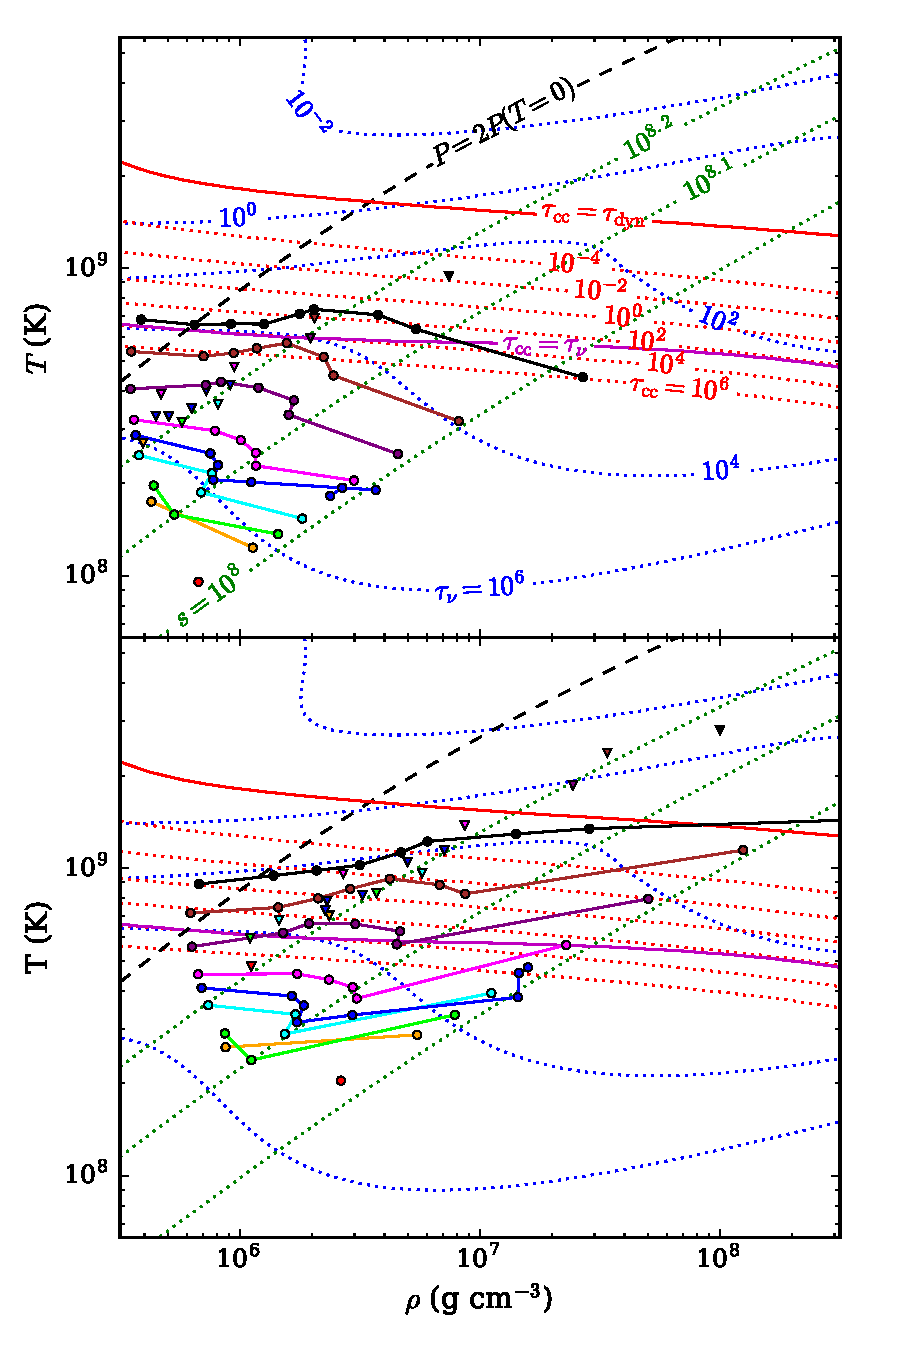
\includegraphics[angle=0,width=0.7\columnwidth]{chapter2_zhu+13/figures/Willitexplode.pdf}
\caption{Top: merger remnant maximum temperature {\Tmax} and corresponding density {\rhoTmax} for all merger remnants.  Values along the equatorial plane are marked with circles, with lines connecting points with the same accretor mass, while values along the rotational axis (only plotted for similar-mass mergers) are marked with triangles (for all, colors indicate accretor mass, encoded as in Fig.~\ref{fig:c2_constacc}).  For similar-mass mergers, equatorial temperatures have been adjusted to account for mixing in convectively unstable cores.  Bottom: maximum temperatures and corresponding densities following estimated post-merger evolution.  The estimate assumes that the remnant spins down completely, that all rotational energy is used to drive matter to large distances, and that the remainder adjusts adiabatically (see text).  Also shown are contours of constant neutrino cooling timescale $\tau_\mathrm{\nu}\equiv C_P T/\varepsilon_\nu$ and carbon fusion heating timescale $\tau_\mathrm{cc}\equiv C_P T/\varepsilon_{\rm CC}$, both in years, as well as entropy $S$ in ${\rm erg\,K^{-1}}$.  (Here, $C_P$ is the heat capacity at constant pressure and $\epsilon$ the specific energy loss/gain rate.)  The lines labeled $\tau_\mathrm{cc} = \tau_\mathrm{\nu}$ and $\tau_\mathrm{cc} = \tau_\mathrm{dyn}$ denote where the carbon fusion heating timescale balances the neutrino cooling and dynamical timescales, respectively.  Finally, the $P = 2P(T$=$0)$ line is shown as an approximate upper bound of the region where degeneracy pressure dominates.  All quantities were calculated using MESA \citep{paxt+11}.}
\label{fig:c2_willitexplode}
\end{figure*}

%\begin{figure}
%\centering
%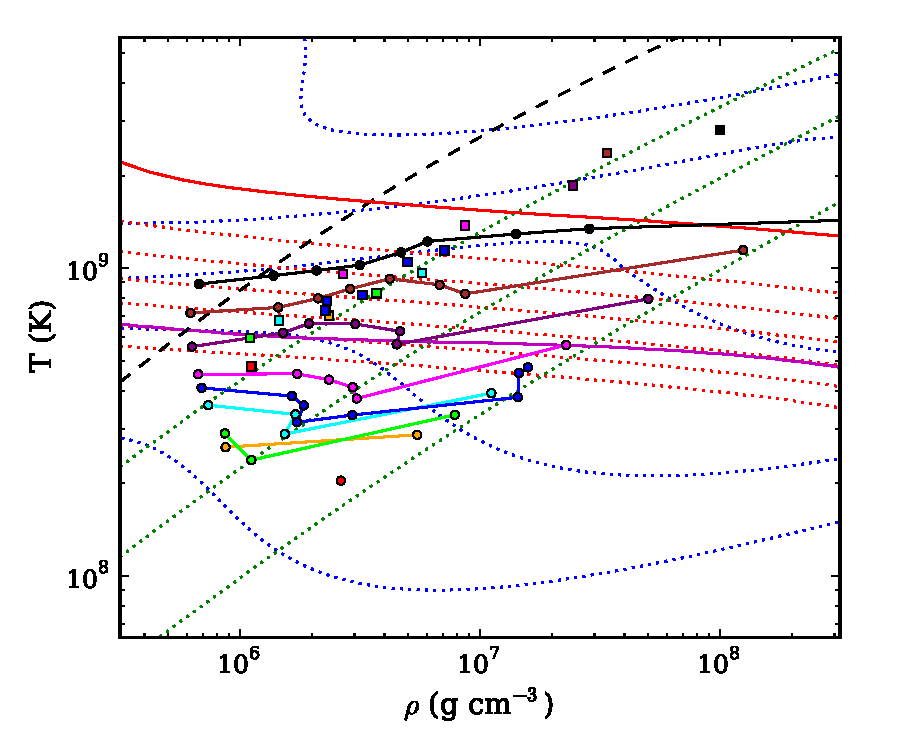
\includegraphics[angle=0,width=1.0\columnwidth]{Willitexplode2.pdf}
%\caption{As Fig. \ref{fig:willitexplode1}, except for maximum temperatures and corresponding densities following estimated post-merger evolution.  The estimate assumes that the remnant spins down completely, that all rotational energy is used to drive matter to large distances, and that the remainder adjusts adiabatically (see text).}
%\label{fig:willitexplode2}
%\end{figure}

%{\bf MHvK: CRAZY idea: for {\em all} mergers, show thin curves of $\Tmax(\phi)$; for dissimilar, this will visually look a bit like the circles, for equal, larger traces}

\begin{figure}
\centering
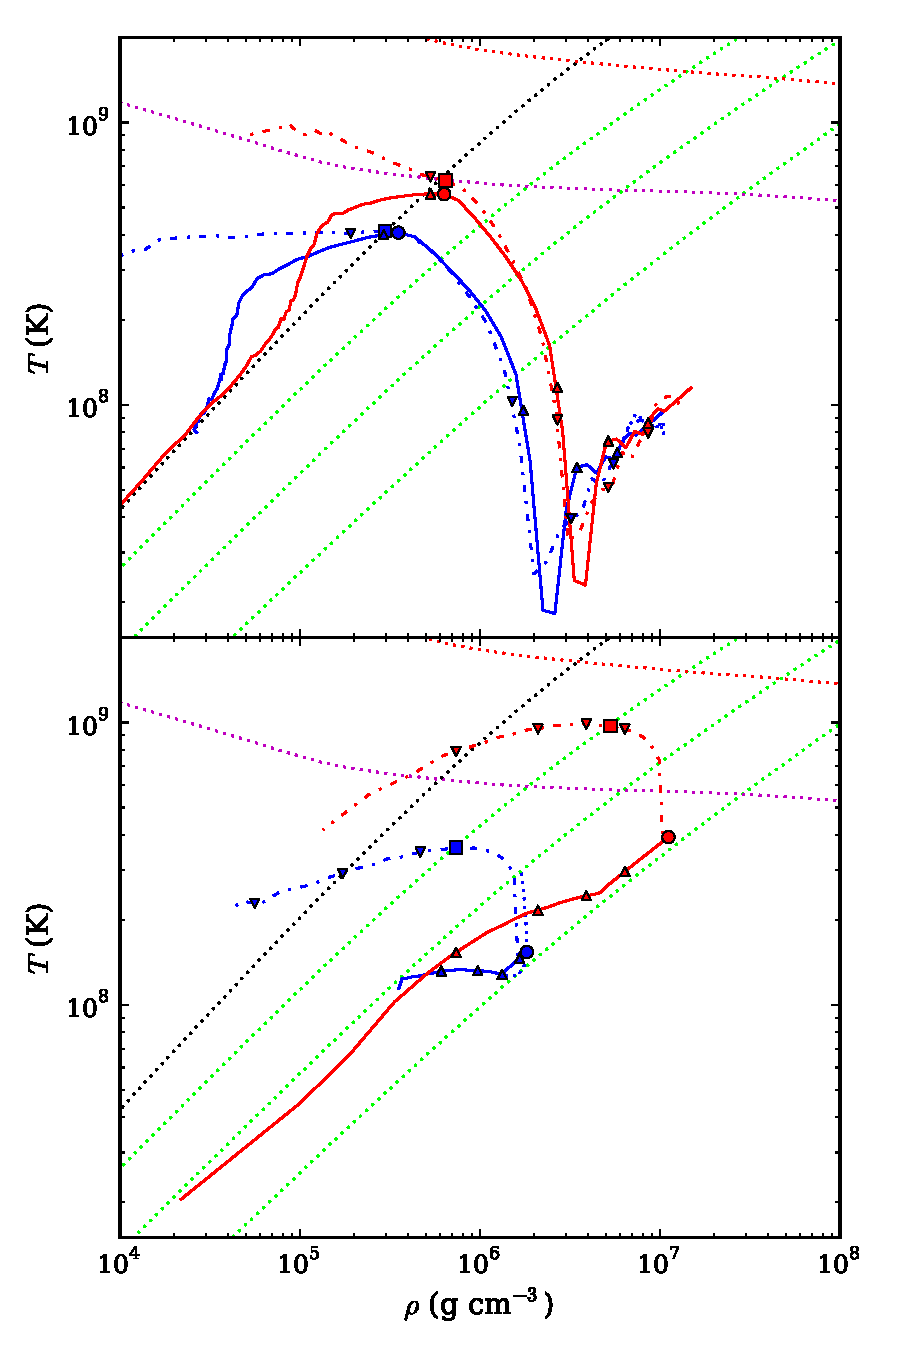
\includegraphics[angle=0,width=0.6\columnwidth]{chapter2_zhu+13/figures/PMEvolution.pdf}
\caption{Estimate of post-merger viscous evolution for 0.4 - 0.8 {\Msun} (top) and 0.6 - 0.6 {\Msun} (bottom) mergers.  In blue are shown the temperature-density structure of the merger remnant, on the equatorial plane before (dotted) and after (solid) correction for convection, as well as along the rotational axis (dot-dashed), with points marking the hottest locations (circles and squares) and steps of 0.2\,\Msun\ in spherical enclosed mass (triangles pointing up and down).  In red, estimates of the structure following viscous evolution are shown, where it is assumed that the remnant spins down completely, that all rotational energy is used to drive matter to large distances, and that the remainder adjusts adiabatically (see text).  For reference, also shown as dotted curves are the contours of constant entropy from Fig.~\ref{fig:c2_willitexplode} (green), as well as the dotted lines where $\tau_\mathrm{cc} = \tau_\mathrm{\nu}$ (magenta), $\tau_\mathrm{cc} = \tau_\mathrm{dyn}$ (red), and $P = 2P(T$=$0)$ (black).}
\label{fig:c2_pmevolution}
\end{figure}

We now turn to the question of how our merger remnants will evolve.  To set the stage, we show in the left panel of Fig.~\ref{fig:c2_willitexplode} for all remnants the maximum temperature \Tmax\ found along the equatorial plane\footnote{The central temperatures for the 0.625 - 0.65 \Msun\ and 1.0 - 1.0 \Msun\ mergers are $\sim\!4$\% and 10\% lower than their respective maximum temperatures.  In both cases, however, the center is much denser than the off-center hotspot, and since our estimated post-merger evolution more greatly affects central material, we show the central equatorial density and temperature for these two systems in Fig. \ref{fig:c2_willitexplode} left, rather than the maximum.} as a function of the corresponding density \rhoTmax.  Here, for the similar-mass mergers for which we found convectively unstable cores (Sec.~\ref{sssec:c2_thermtrends}), we show the (lower) temperatures reached after artificially mixing them.   For those mergers, the much higher temperatures reached along the rotational axis are shown as well (triangles).  One sees the trends identified earlier: \Tmax\ is mostly set by the accretor, while \rhoTmax\ depends more strongly on the donor.  As a result, maximum temperature occurs in less degenerate conditions for dissimilar-mass mergers, crossing the degeneracy line for our most disparate cases.  One also sees that for all but the most massive accretors, carbon fusion will not start: the neutrino cooling time is shorter than the fusion heating time.  This is consistent with what was found in previous work (see Sec.~\ref{sec:c2_intro}).

\subsection{Viscous Evolution and Possible Spin Down}
\label{ssec:ch2_viscevo_possiblespindown}

Following the merger, processes that happen on timescales slower than the dynamical time can become important.  These include viscous evolution, neutrino emission, radiative or convective thermal adjustment, and magnetic dipole radiation spin-down.  Out of these, convection acts on the fastest timescale, and we already included its effect on the core in Fig.~\ref{fig:c2_willitexplode} left.  Next fastest would almost certainly be viscous evolution.  The merger remnant is unstable to both the magneto-rotational instability \citep{balbh91} and Tayler-Spruit dynamo \citep{spru02}.  Radiative adjustment is expected to be much slower, except at the surface, where radiative losses may also lead to convection in some systems \citep{shen+12,schw+12,rask+12}.  Using the standard \cite{shaks73} $\alpha$-prescription for the viscosity $\nu = \alpha c_s H$, where $c_s$ is the local sound speed and $H$ is the scale height of the system, the viscous evolution timescale for the remnant disk is
\begin{equation}
t_\mathrm{visc} = \frac{R_\mathrm{disk}^2}{\nu} = \frac{1}{\alpha}\left(\frac{R_\mathrm{disk}}{H}\right)^2t_\mathrm{dyn} \sim \frac{10}{\alpha}t_\mathrm{dyn},
\end{equation}
implying a timescale $t_{\rm visc}\sim10^3-10^5{\rm\,s}$ for $\alpha\sim10^{-3}-10^{-1}$ and $t_\mrm{dyn} \sim 10$ s.  This is orders of magnitude smaller than both the neutrino loss timescale ($\gtrsim\!10^3$ yrs; see Fig.~\ref{fig:c2_willitexplode} left) and thermal adjustment timescale ($\gtrsim\!10^4$ yrs; \citealt{shen+12}).

It is possible that the strong differential rotation during a merger results in substantial amplification of magnetic fields.  The one known probable WD merger remnant, RE J0317$-$853, has a surface magnetic field of $3.4\times10^8\,$G \citep{bars+95,kube+10}.  If mergers lead to strongly magnetized WDs, and these WDs additionally drive an ionized outflow, the magnetic coupling between the outflow and the WD could serve to transport angular momentum out of the system, spinning down the WD.  The timescale for such a spin-down is roughly given by,
%
\begin{equation}
t_\mathrm{msd} \sim \frac{L}{\dot{M}R_A^2\Omega}
              \sim \frac{L}{(\dot M\Omega)^{3/5}(B^2R^6)^{2/5}},
\end{equation}
%
where $L$ is the angular momentum of the remnant, $\dot M$ the mass loss rate, $R_A$ the Alfv\'{e}n radius, and $\Omega$ the angular spin frequency.  For the second approximation, we used that $R_A\sim (B^2R^6/\dot M\Omega)^{1/5}$, with
$B$ the surface magnetic field and $R$ the remnant radius.  Scaling to  $B=B_810^8\,$G and $\dot M={\dot M}_{-7}10^{-7}\,\Msun{\rm\,yr^{-1}}$ (similar to what is observed for RE J0317$-$853 -- see above -- and [WR] cores of planetary nebulae [\citealt{hama97}]), and using the properties inferred for a 0.6 - 0.6 \Msun\ remnant ($L\simeq L_{\rm tot}\simeq10^{50.5}{\rm\,g\,cm^2\,s^{-1}}$, $R\simeq R_{\rm disk}\simeq10^9{\rm\,cm}$, $\Omega\simeq\Omega_{\rm max}\simeq10^{-0.3}{\rm\,s^{-1}}$, we find $t_{\rm msd}\simeq8\times10^3\,B_8^{-4/5}{\dot M}_{-7}^{-3/5}{\rm\,yr}$, which is of the same order as the neutrino cooling timescale of $\sim\!10^4{\rm\,yr}$ at the ignition line (for the whole range of remnants, $2\times10^3\lesssim t_{\rm msd}\lesssim 5\times10^4{\rm\,yr}$).

Accretion from the disk, loss of rotational support, and possible cooling of the hot envelope could all compress and heat the remnant core.  A detailed study of this is beyond the scope of this paper, but we can make first-order estimates of the effects on our merger remnants, and compare these with the more detailed analysis of \cite{schw+12} in one specific case.

For our estimates, we make four assumptions: (i) spin-down and accretion are much faster than thermal processes, and do not lead to local dissipation (i.e., particles entropies are constant in time); (ii) all angular momentum is carried away to large distances; and (iii) corresponding matter ends up with zero total energy (i.e., is at large distances and has negligible kinetic and internal energy).  From energy conservation, the last assumption implies that the remaining object will have the same total energy as our merger remnant (but a lower mass), the first that it will have the same entropy structure, and the second that it has no rotational support.  To determine the properties, we first determine the entropy profile of the merger remnant, by averaging entropy over isopotential surfaces.  We then use this entropy profile and an estimated central density to construct a spherically symmetric (non-spinning) hydrostatic model, iterating on the central density until it has the correct total energy (inside of the zero-pressure surface).  This automatically gives the mass contained in this object, which will be lower than our remnant mass, the remainder representing material that, due to dissipation of rotational energy, has expanded out to large distances and therefore provides negligible weight.  To determine the evolution of hot spots, we order remnant particles by potential, and map them to their new positions in the final object, calculating new temperatures from the new densities, again assuming their entropy did not change (entropy is not constant over isopotential surfaces, so these temperatures are not strictly consistent with the hydrostatic model).

In Fig.~\ref{fig:c2_pmevolution}, we show the results of our evolutionary estimate for our fiducial 0.4 - 0.8 and 0.6 - 0.6 {\Msun} systems.  For the former case, the core-envelope, originally 0.90\,\Msun, accretes 0.06\,\Msun\ from the disk, the remaining 0.25\,\Msun\ going to large distances.  The central core is not significantly heated, while the lower-density hot envelope is, with the outer hot envelope along the rotational axis passing the ignition line.  Since this material is almost non-degenerate, the resulting nuclear burning will likely be stable, or be extinguished by expansion.  Thus, not unexpectedly, the hot envelopes of dissimilar-mass mergers are not good candidates for a nuclear runaway.  

%MHvK: I removed: As loss of rotational support should result in compression mainly along the equatorial plane, much of the rotational axis hot envelope may instead remain unperturbed, or be squeezed out to larger distances and adiabatically cool.

For the 0.6 - 0.6 {\Msun} system, the center of the final, spun-down object is at much higher density and temperature than the remnant, while much of the outer regions have become less dense and cool.  The latter happens because similar-mass mergers have strong rotational support, and if this is removed their binding energy increases significantly.  To compensate for this, a large amount of mass has to expand to large distances, causing the core-envelope mass to decrease from 1.11 {\Msun} to 0.91 {\Msun}.  In the final object, the hottest point on the equatorial plane does not reach the ignition line, but the significantly hotter points above and below the equatorial plane do, at densities under which degeneracy pressure still dominates.  Hence, if the hot spots indeed compress with the rest of the remnant, a nuclear runaway could be triggered.  (Of course, a nuclear runaway would start as soon as the heating timescale becomes shorter than the compression timescale, which may happen closer to the ignition line.)

%MHvK: removed the sentence below since we do not really know the timescale; see added sentence above.  I also think we should remove the yellow line (perhaps instead include some heating timescale lines)
%The assumptions for our estimate break down for any degenerate points in the remnant that reach past the yellow $\tau_\mathrm{cc} = 10^{-4}$ yr curve: at this point the nuclear burning timescale becomes smaller than the viscous evolution timescale, and it becomes important to consider nuclear energy generation in addition to accretion, but at this point a nuclear runaway has occurred.

In the right panel of Fig.~\ref{fig:c2_willitexplode}, we show the results of applying our estimates to all our merger remnants.  One sees that all compress and heat, and almost every remnant whose accretor mass is above 0.8\,\Msun\ will reach ignition somewhere on the equatorial plane, in many cases under degenerate conditions.  We also chart the evolution of the off-center hot spots in similar-mass mergers (square points), and while they are at lower density, they remain degenerate and are all pushed substantially further above the ignition line than their counterparts on the equatorial plane.  Almost all similar-mass mergers with an accretor mass above 0.5 {\Msun} could therefore experience nuclear runaways due to their hot spots, though at least some of them will become non-degenerate before an explosion can occur.

The above suggests it is at least plausible that many of our mergers would eventually ignite in degenerate conditions, and that it thus is worthwhile to simulate their evolution in detail.  Suitable simulations have recently been pioneered by \cite{shen+12} and \cite{schw+12}.  \citeauthor{shen+12} started with a one-dimensional simulation, where they ported the remnant of a 0.6 - 0.9 {\Msun} merger (from \citealt{dan+11}), and evolved it assuming a $\gamma = 5/3$ polytropic equation of state and an $\alpha = 10^{-2}$ viscosity.  They find the system spins down completely due to outward angular momentum transport, and the rotationally-supported thick disk is transformed into a tenuous, thermally-supported envelope that hardly affects the core.  Over longer, thermal evolution timescales (simulated using MESA, \citealt{paxt+11}), this tenuous hot envelope cools, compresses the core, and lights off-center convective carbon burning, eventually turning the remnant into an ONe WD (that may end its life in an accretion induced collapse).

\cite{schw+12} went a step further, porting the same 0.6 - 0.9 {\Msun} simulation, as well as seven other systems, into two-dimensional ZEUS-MP2 simulations \citep{haye+06}, using the Helmholtz equation of state and an $\alpha=3\times10^{-2}$ viscosity.  They confirm the one-dimensional results, finding complete spin-down and transformation of the rotationally supported disk into a tenuous, spherically symmetric, hot envelope.  They find a 50\% increase in the temperature of the hottest point, and a factor of 3 increase in the corresponding density.  They also find entropy to roughly be constant in the remnant, except in the outer regions and at the very center, where dissipation of rotational energy leads to heating.

It is encouraging that the results of the above detailed simulations are similar to what we find using our first-order estimates.  For our 0.6 - 0.9 {\Msun} remnant, our estimate give increases for the hottest equatorial point of a factor of 2.5 in density and 1.6 in temperature, reasonably close to what is found by \citeauthor{schw+12}\footnote{For the hottest point along the rotational axis, we find a factor of 4.8 increase in density and 2.1 increase in temperature, suggesting our model does not depict as well the evolution of the outer hot envelope along the rotational axis.}.  Thus, our simplifying assumptions appear to be appropriate at least for dissimilar-mass mergers, where most of the rotational dissipation will be in the disk and envelope, and the structure of the remainder is roughly spherically symmetric (both in density and temperature).  It is not clear our estimates would be equally good for similar-mass mergers, where rotational dissipation should occur throughout the star, heating the entire remnant, and where there are substantial differences between the remnant's density and temperature structures.  In particular, the rotational axis hotspots may dissipate, which would potentially make it more difficult for a similar-mass system to achieve a runaway.  It will thus be particularly interesting to simulate the further evolution of those remnants in more detail.  Unfortunately, no such remnants were included by \citeauthor{shen+12} and \citeauthor{schw+12}.

\subsection{Possible Explosions?}

From our estimates, it seems that, as suggested by \citeal{vkercj10}, many merger remnants will ignite carbon fusion.  If a detonation is triggered, the resulting explosion may well resemble an SN Ia.  Indeed, if the remnants spun down before ignition, their structures are sufficiently close to that of a cold WD that the calculations of \cite{sim+10} should apply.  From our estimates, for mergers that have a total mass between 1.2 and 1.4\,\Msun\ (which should be the most common ones), the final objects have masses between $\sim\!0.9$ and $\sim\!1.1$ \Msun\, which matches fairly nicely the range of $\sim\!1$ to $\sim\!1.2$ \Msun\ required to reproduce the observed range of SN Ia luminosities \citep{sim+10}.

%MHvK: I think this is a bit too much detail, where we  add relatively little; replaced by a single sentence above

Of course, it is far from clear whether ignition leads to a detonation, since we do not currently understand how detonations are triggered (\citealt{seit+09,woos+11}, and references therein).  Generally, it should help that ignition in our remnants is at much lower density (a few $10^7\,{\rm\,g\,cm^{-3}}$) than is the case for near-Chandrasekhar models ($\sim\!10^9{\rm\,g\,cm^{-3}}$), because complete burning leads to much larger relative overpressures (e.g. \citealt{mazumw77}; \citealt{seit+09}).  Also, if a deflagration is started, plausible mechanisms to transition to a detonation all seem to require densities around $10^7\,{\rm\,g\,cm^{-3}}$, where the conductive flame speeds are slower and the separation between the various burning fronts increases (e.g., \citealt{woos+09,woos+11}).

An interesting aspect of our results is that for all cases ignition likely happens off-center: in shells for dissimilar-mass mergers and in hot spots along the rotational axis for similar-mass ones.  Previous one-dimensional simulations suggested off-center ignition would lead to a slow deflagration flame that turns the CO WD into a ONe WD (e.g., \citealt{saion85}).  However, these calculations assumed a hot spot many pressure scale heights above the center.  For ignition closer to the center, a deflagration plume is produced (e.g., \citealt{aspd+11}), which may transition to a detonation \citep{seitcr11} and unbind the star.   

Given our findings, it seems likely that, if a detonation occurs, it will be triggered off-center.  It would be interesting to simulate the resulting explosion, and see whether one could reproduce the observational evidence for asymmetries, which have been interpreted in terms of off-center ignition (though so far only in the context of near-Chandrasekhar models; \citealt{maed+10a,maed+10b}).

Finally, while we simulated only mergers of CO WDs, we can extrapolate our results to more massive ONe WDs.  For these, the temperatures would be at least as high as for our 1\,\Msun\ accretors, and, after further viscous evolution, the mergers should become hot enough to ignite Ne burning.  If this also leads to a detonation, the lower fusion energy released would likely lead to a less energetic explosion than expected for a CO WD merger, but it would produce far more $^{56}$Ni and have a very large mass.  Plausibly, it would resemble an SN Ia like SN 2009dc, which had unusually low ejecta velocities, produced $\sim\!1.8\,\Msun$ of $^{56}$Ni and had a total ejecta mass of $\sim\!2.8\,\Msun$ \citep{taub+09}.

%\subsection{Future Work}

%In Sec. \ref{ssec:initcond} we noted that we use approximate initial conditions, and it has been shown \citep{dan+12} that accurate initial conditions non-negligibly affect the structure of the merger remnant.  As discussed in Sec. \ref{ssec:varyingazero}, to first order we expect the extended period of quasi-stable mass transfer found in initial condition studies would result in more mergers across our parameter space resembling dissimilar mass mergers, since at final coalescence the donor would have become less massive, and the accretor more.  This could reduce the number of systems in our parameter space study that would resemble similar mass mergers, particularly if more than $\sim0.1$ {\Msun} is generally transferred before coalescence.  If the amount of mass transferred depends on total system mass (rather than just {\qrho}), then the homologies we presented in Sec. \ref{ssec:samplingofmergers} would also be affected.  No study of how accurate initial conditions for unsynchronized systems has thus far been published.  We are in the process of generating accurate initial conditions for our unsynchronized systems in order to quantify how the trends we have found would be affected.

%The structure of the remnant is affected by whether or not the merging binary was synchronized, a still-unresolved issue (Sec. \ref{ssec:compwithothers} \emph{PERHAPS WE SHOULD MOVE THAT ENTIRE DISCUSSION HERE, SINCE WE DON'T COMPARE WITH ANYONE EXCEPT LOREIG ANYMORE??}).  Perhaps the most effective way of investigating this issue is with observation.  Two very short (period on the order of minutes) binary systems are known to be eclipsing \citep{stei+10,brow+11}, allowing in principle measurement of the rotational velocity modulo the inclination to the observer (which may be different than the inclination of the orbital plane), $v\sin i$, of both stars through the Rossiter-McLaughlin effect.  Rotation could also be measured through the broadening in the narrow, non-LTE core of H$\alpha$.  We are currently performing such measurements on SDSS J065133.33+284423.3, in order to compare with theoretical tidal dissipation models.

%To determine the fate of our merger remnants, we must simulate the post merger evolution of our parameter space.  \citeauthor{schw+12} have already demonstrated the effectiveness of 2.5D grid-based simulations in realistically describing this evolution.  We are currently preparing to port our remnants into a code similar to that of \citeauthor{schw+12}'s, in order to extend their work by filling out the parameter space of CO WD mergers.  Most critically, we will simulate the evolution of similar mass mergers, which is missing from \citeauthor{schw+12}.  The entire structure of an similar mass merger remnant would be affected by spin-down (only the outer envelope is greatly affected for dissimilar mass mergers), and our estimates above indicated that these systems are most likely to experience a core nuclear runaway when compressed.

%Ultimately, the physical robustness of \citeal{vkercj10}'s SN Ia channel also depends on whether or not, even if a detonation can be triggered in an evolved remnant (Sec. \ref{ssec:postmerger}), the resulting explosion can reproduce observationally established properties of SNe Ia.  \cite{sim+10}'s are of bare, cold sub-{\Mch} WDs.  True merger remnants feature material in extended tenuous envelopes, and possibly outflows.  If the remnant core produced an SN Ia, the explosion ejecta will shock heat this material, changing the early-time light curve of the SN Ia \citep{frye+10}.  Because they are insufficiently dense and are thought not to have an extended deflagration phase before detonating, sub-{\Mch} objects also cannot produce stable $^{58}$Ni from electron capture during the explosion.  $^{22}$Ne pollution from burning of CNO cycle catalysts, however, can result in stable nickel production in the pure detonation of sub-{\Mch} WDs, though the amount generated, and the signature imprinted in the SN Ia's spectra, will differ from those of electron capture.  Since [Ni II] lines are indeed seen in the late-time spectra of SNe Ia \citep{gera+07, maed+10a}, it is not yet obvious which stable nickel generating method is more favored by observations (see discussion in \citealt{vker12}).  These questions remain to be investigated with regard to \citeal{vkercj10}'s channel.

%Stable, relatively slow moving $^{58}$Ni has been sighted in late-time SNe Ia spectra (ex. \citealt{gera+07}).  $^{58}$Ni can be generated either through electron capture during nuclear burning in high-density material, or by burning $^{22}$Ne.  While $^{22}$Ne is expected to gravitationally settle to the center of single WDs, it will re-mix during a merger, and in \citeal{vkercj10}'s channel there is insufficient time for it to settle before an explosive nuclear runaway occurs.  This means that, if an SN Ia occurs, the $^{22}$Ne distribution generated by the merger will determine where $^{58}$Ni is generated during the explosion.  There is therefore the potential for spectroscopic features distinguishing explosions due to \citealt{vkercj10}'s SN Ia channel from those due to other channels.  We are currently exploring the fate of the He atmosphere and Ne pollutants using tracer particles in our simulations.

\section{Conclusion}

We have performed a large, detailed parameter-space study of CO WD mergers, extracting pertinent properties and profiles for each remnant, and studying how these vary across parameter space.  For a merger involving dissimilar-mass WDs, with low {\qrho} = {\rhocrat}, the outcome is a cold, slowly rotating, degeneracy-supported remnant core, which is essentially unaffected by the merger, surrounded by a hot, roughly spherical envelope and, further out, by a sub-Keplerian disk.  For a similar-mass merger, with high {\qrho}, an ellipsoidal core is produced along with a small disk, and the entire remnant is hot and partly supported by rotation.  The transition between these two regimes is smooth, but occurs roughly at $\qrho\simeq0.6$, or equivalently a mass difference $\Delta M= \Ma-\Md \simeq 0.1$.  We found that for a fixed {\qrho}, merger remnant curves are roughly homologous.  We also presented trends for a number of merger remnant properties, providing linear scaling relations and best fits for most of them, hoping these can guide theoretical understanding and help analytical estimates.

We made first-order estimates of the post-merger viscous evolution and spindown, and found that it is plausible that a large fraction of the mergers simulated will eventually experience a nuclear runaway, as was suggested by \citeal{vkercj10}, and thus possibly end as thermonuclear supernovae.  Further, detailed, simulations of this evolution across the whole parameter space, using techniques similar to those of \citet{shen+12} and \citet{schw+12}, would be required to confirm this.  If the evolution of these remnants results in a detonation, a detailed comparison of the resulting light curve with observations must be carried out.

Our work represents one of the most detailed parameter studies of WD mergers to date.  It would benefit, however, from resolution of a number of topics.  First, for greater precision, it will be necessary to use better initial conditions.  For synchronized systems, it is already known this has nontrivial effect on the outcome \citep{dan+11,dan+12}, and our results suggest it is important also for non-synchronized systems.  Unfortunately, for the non-synchronized case, it is not trivial to implement the initial conditions, but better approximations are possible.  Second, it would be useful to try to compare with merger simulations done with a grid code, which should have become more straightforward now that good moving mesh codes have become available \citep{spri10,duffm11}.  More generally, whether or not WDs are synchronized before the merger remains unknown, yet clearly affects the resulting merger.  Hopefully, this can be resolved empirically, by measuring the spin frequency for WDs in the very short-period binaries that have recently been discovered (e.g., \citealt{brow+11}).

\vspace{5mm}

We thank Pablo Lor\'{e}n-Aguilar, Enrique Garc\'{i}a-Berro, Stuart Sim, Enrico Ramirez-Ruiz, Marius Dan, James Guillochon, Evan Scannapieco, Cody Raskin and Ken Shen for insight into their simulations and useful discussion on the physics of mergers and post-merger evolution.  We are grateful to Frank Timmes for creating the Helmholtz equation of state, and assisting us with its implementation in Gasoline, as well as to Bill Paxton and the MESA team for creating MESA and making it modular.  This work made extensive use of NASA's ADS and was supported by the Vanier and Discovery grants of Canada's Natural Sciences and Engineering Research Council (NSERC).

\section{Postscript: Post-Merger Evolution Revisited}
\label{sec:c2_postscript}

Since the publication of Ch. \ref{ch:ch2} as \citeal{zhu+13}, others have done work on the viscous evolution of merger remnants.  \cite{rask+14} uses the machinery of \cite{schw+12} to generate post-viscous remnant profiles for massive (mostly dissimilar-mass) mergers with $>0.9\,\Msun$ accretors, to determine their nucleosynthetic output if they then experienced a pure detonation.  They do not discuss their viscous simulations in detail.  Also published was \cite{ji+13}, a work of particular relevance to our investigations not only because they simulate the post-merger evolution of an equal-mass $0.6-0.6\,\Msun$ remnant, but also because they eschew the use of an $\alpha$-viscosity and instead directly evolve the magnetic field of the merger remnant.  We have not performed our own post-merger evolution simulations\footnote{We experimented with \flash-based 2.5D simulations that included an $\alpha$-viscosity, but did not follow up with a detailed investigation.}, and use \cite{schw+12} and \cite{ji+13}'s results extensively throughout this thesis.  Since this thesis has no dedicated chapter on post-merger evolution, we expand and update the discussion in Sec. \ref{ssec:ch2_viscevo_possiblespindown} below with \cite{ji+13}'s results.

%\cite{shen+12} flesh out the further evolution of \cite{dan+11}'s $0.6 -0.9\,\Msun$ dissimilar-mass merger.  They first use a 1D Lagrangian hydrodynamic simulator with a $\gamma = 5/3$ polytropic equation of state to evolve the (height-integrated) remnant surface density profile under the influence of a uniform $\alpha = 10^{-2}$ viscosity prescription.  This $\alpha$ value is chosen so the system evolves over $t_\mrm{visc} \sim 10^{4}\,\mrm{s}$, roughly consistent with the viscosity arising from either the magnetorotational instability (MRI; \citealt{balbh91}) or (in region where its onset is unfavourable) the Tayler-Spruit dyanamo (eg. \citealt{spru02}).  Material inside of $M_\mrm{enc} = 0.9\,\Msun$ is assumed to remain unchanged.  Note that $\alpha$ is likely to be non-uniform in space and time, as, for example, the Tayler-Spruit dynamo viscosity will not be identical to that of the MRI, but \cite{shen+12} argue this will only change the details of the evolution -- the qualitative results remain unchanged so long as the viscous timescale falls between the dynamical and thermal ones.  They find -- as expected from viscous evolution -- evolution toward a shear-free solid body rotation, with the sub-Keplerian disk converted to a thermally supported, near-virial, tenuous atmosphere.  This atmosphere ($\rho \lesssim 10^4\,\gcc$, $T \sim 10^9\,\mrm{K}$) is radiation-dominated, and so has a near-Eddington luminosity.  

%  Since the $0.6 - 0.9\,\Msun$ merger has a cold core with little rotational support, the loss of this support does not heat it substantially; the hottest point in the remnant is instead a ``hot ring'' residing at the boundary between the $0.9\,\Msun$ accretor and disrupted donor material, formed by shock-heated donor material falling onto the accretor.

%\cite{schw+12} replace \cite{shen+12}'s Lagrangian solver with the \textsc{ZEUS-MP2} \citep{haye+06} Eulerian hydrodynamics code, modified with the Helmholtz \citep{timms00} equation of state, a stress-tensor term with a dynamic viscosity coefficient given by $\alpha = 3\times10^{-2}$ ($\alpha = 10^{-4} - 10^{-1}$ lead to qualitatively similar end results) and a simplified five-isotope nuclear network.  They simulate eight dissimilar-mass merger remnants (from \citealt{dan+11}), including two CO-CO ones, and confirm \cite{shen+12}'s qualitative results, most notably that a combination of spin-down and viscous heating converts the rotationally-supported outer layers of the remnant to a spherically symmetric, thermally-supported and convectively unstable hot atmosphere.  For their fiducial $0.6 - 0.9\,\Msun$, spin-down increases the hot ring's temperature by a factor of $\sim1.5$, and density by a factor of $\sim3$, enough to push it above the carbon ignition line.  The other remnants they consider are either remnants of He-CO mergers with extreme mass ratios, those of low-mass He-He mergers, or massive, $\gtrsim1.7\,\Msun$ ones.  The results of these systems are very similar to their fiducial one, except for the contribution of He nuclear burning to the temperature structure of the spun-down remnant for He-CO remnants.

\cite{ji+13} run 2.5D magnetohydrodynamic simulations with the Eulerian grid code \flash\ \citep{fryx+00}, using the $0.6 - 0.6\,\Msun$ remnant of \citeal{loreig09} as initial conditions.  They utilize a axisymmetric cylindrical grid and the Helmholtz EOS.  Since \citeal{loreig09}'s remnants are unmagnetized, they artificially insert a purely poloidal magnetic field whose strength is $\sim10^8\,\mrm{G}$ in the remnant disk, and $\lesssim10^5\,\mrm{G}$ in the core (they determine their results are robust to changing initial field strength and spatial resolution by factors of 2).  They advance their simulation to $2\times10^4\,\mrm{s}$, comparable to the completion times in \cite{schw+12}.  They find that the magnetorotational instability (MRI) acts on the differentially rotating portions of the remnant to greatly amplify the field over several hundred seconds, until it reaches equilibrium with a peak field strength of $\sim10^9\,\mrm{G}$ in the disk and $\gtrsim10^{10}\,\mrm{G}$ in the core, as well as a total magnetic energy of $\sim10^{48}\,\mrm{erg}$, on par with the differential rotation energy of the system (see Ch. \ref{ch:ch4}).  This field produces Maxwell stresses that are roughly equivalent to a $\alpha \sim 10^{-2}$ viscosity, facilitating global outward angular momentum transport like in \cite{schw+12}.  It also generates a hot, magnetized corona by displacing disk material through magnetic buoyancy, and a biconal outflow along the remnant's rotational axis.  These outflows eject $10^{-3}\,\Msun$ of material at roughly twice the local escape speed (of $\sim1600\,\mrm{km}\psec$).  

Much like \cite{schw+12}, \cite{ji+13} find that the remnant loses most of its rotational support and evolves toward a spherically symmetric state with a dense, degeneracy-supported core and a more tenuous thermally-supported envelope.  By the end of the simulation $\sim0.08\,\Msun$ of material either resides in the magnetically dominated corona or has left the simulation domain, leaving $1.12\,\Msun$ remaining in the remnant, with $1.07\,\Msun$ of this residing within $r = 1.5\times10^9\,\mrm{cm}$ in the dense core (\bobjiprivcomm).  Accretion onto and loss of rotational support within the core leads to its center being compressionally heated by a factor of $\sim2.5$ in density and $\sim2$ in temperature.  As their initial conditions are a factor of $\sim2$ hotter than our $0.6 - 0.6\,\Msun$ remnant (Sec. \ref{ssec:c2_compwithloreig}), this additional compression ignites central nuclear fusion.

% The central density of schw+12's 0.6 - 0.9Msun remnant comes from Table 1 of dan+11; the spun-down value comes from Table 3 of schw+12.  For the 0.6 - 0.6 system, we use the central term in the xy-plane temperature-density relationship ("crho" and "cT" if using GitHubTemp/PaperRunaway/papercalc_other.py) rather than the max values.

We can compare the results of \cite{ji+13}, along with \cite{schw+12}, to our simple estimates of viscous evolution in Sec. \ref{ssec:ch2_viscevo_possiblespindown}.  The most relevant quantities are the density and temperature at the center and at the hottest point of the post-viscous remnant, to determine whether carbon fusion ignites under highly degenerate conditions and the amount of material that remains a part of the dense, degeneracy-dominated remnant core.  The latter is important for comparing against simmering WDs in Chapter \ref{ch:ch5}.  As stated in Sec. \ref{ssec:ch2_viscevo_possiblespindown}, we estimate the hottest point within our $0.6-0.9\,\Msun$ remnant increases by a factor of $2.5$ in density and $1.6$ in temperature, very similar to \cite{schw+12}'s results.  The central density of their remnant is $1.75\times10^7\,\gcc$ at the start of viscous evolution \citep{dan+11} and $2.8\times10^7\,\gcc$ at the end -- an factor of $1.6$ increase, while we find a factor of $2.0$.  We tend to estimate much larger amounts of compressional heating for similar-mass systems, however, finding that the $0.6 - 0.6\,\Msun$ one increases its central density and temperature by a factor of $6.6$ and $2.7$, respectively, substantially larger than the factors of $\sim2.5$ and $\sim2$ found by \cite{ji+13}.  Similarly, \cite{rask+14} find the central density of their $1.0-1.0\,\Msun$ remnant increases from $7.1\times10^7\,\gcc$ to $2.4\times10^8\,\gcc$, a much smaller compression than the factor of $\sim10$ we find.  This is likely because our simple estimates assume all rotational energy is deposited as heat solely in the outermost regions of the remnant, while in reality remnants, particularly those of similar mass, are rotationally supported throughout and thus will likely also be heated throughout during viscous evolution, reducing the amount of core compression and associated compressional heating.  We also note \cite{ji+13}'s remnant also has not fully lost core rotational support at the end of their simulation\footnote{We do not know if the same is true for \cite{rask+14}'s simulations.  \cite{ji+13} additionally note the central temperature at the end of evolution has not converged, increasing by $\sim20$\% with spatial resolution.}, still having $\Omegac \approx 0.15\,\psec$.  We conclude our estimates are reasonable dissimilar mass systems, but overestimate by a factor of a few the degree of compression and heating in similar-mass ones.

%There are unfortunately no other systems we can directly compare to, but we are able to use more of \cite{schw+12}'s results to determine the mass of the post-viscous core. 

\begin{figure}
\centering
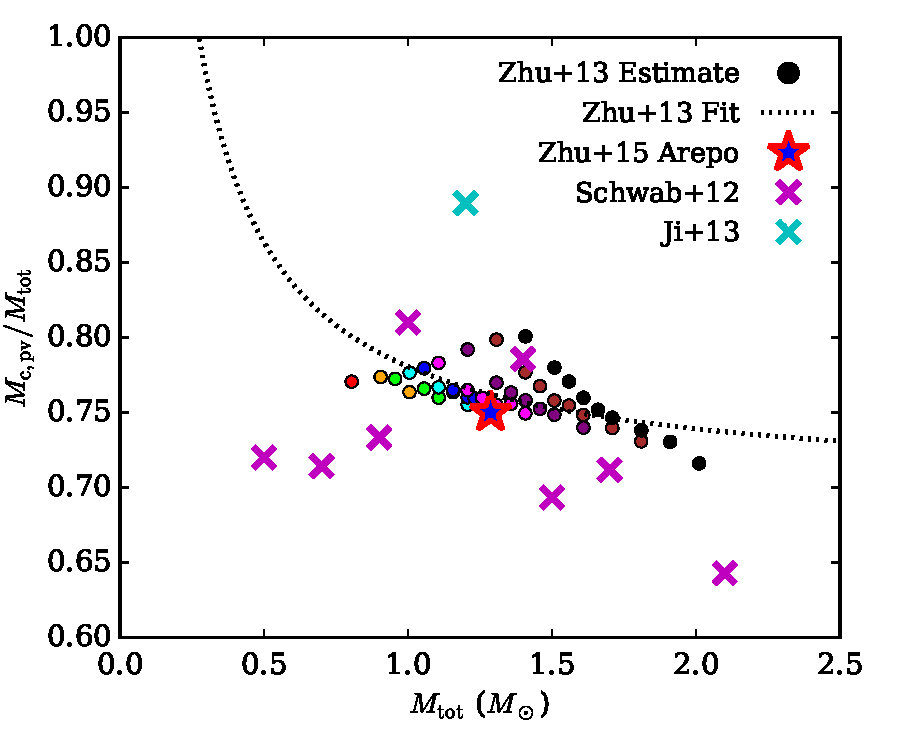
\includegraphics[angle=0,width=0.6\columnwidth]{chapter2_zhu+13/figures/c2a_mcpv.pdf}
\caption{Ratio of post-viscous degenerate core mass \Mcpv\ -- estimated using the simple viscous evolution prescription in Sec. \ref{ssec:ch2_viscevo_possiblespindown} -- to the remnant total mass \Mtot\ as a function of \Mtot\ for the systems of Ch. \ref{ch:ch2} (points; colors have the same meaning as in Fig. \ref{fig:c2_willitexplode}) and the $0.625 - 0.65\,\Msun$ remnant from the \arepo\ MHD simulation (Ch. \ref{ch:ch4}; red-blue star).  Also plotted are estimates of $\Mcpv/\Mtot$ from \citeauthor{schw+12} (\citeyear{schw+12}; using $M_\mrm{c} + M_\mrm{tp}$ in their Table 3) using magenta Xs and \cite{ji+13} using a cyan X.  The dotted line is a best fit to the Ch. \ref{ch:ch2} points given by Eqn. \ref{eq:c2a_mfit}.}
\label{fig:c2a_mcpvvsmtot}
\end{figure}

In our simple estimate, the mass of the post-viscous core, \Mcpv, is given by the mass of the spherically symmetric hydrostatic model representing the spun-down remnant (Sec. \ref{ssec:ch2_viscevo_possiblespindown}).  In Fig. \ref{fig:c2a_mcpvvsmtot}, we plot the ratio of \Mcpv\ to the total mass \Mtot\ of the merging binary, as well as a linear fit to the $\Mcpv-\Mtot$ relationship,

\eqbegin
\Mcpv = 0.70\Mtot + 0.08\,\Msun.
\label{eq:c2a_mfit}
\eqend

\noindent  We also perform our estimate on the $0.625 - 0.65\,\Msun$ remnant from our \arepo\ \citep{spri10} MHD simulation in Ch. \ref{ch:ch4}, and find little difference from its \gasoline\ counterpart.  For \cite{schw+12}, we estimate \Mcpv\ as the combined mass of the core and isothermal region ($M_\mrm{c} + M_\mrm{tp}$) in their Table 3.  We find these follow the overall pattern of our estimates, but tend to be $\sim0.05\,\Msun$ below it.  For \cite{ji+13}, $\Mcpv \approx 1.07\,\Msun$ (see above), which is $\sim0.15\,\Msun$ above our estimate.  Our estimate therefore only roughly reproduces (with errors of $\sim0.1\,\Msun$) the amount of mass remaining in the post-viscous core, partly because the assumption that material not in the core is marginally bound with $E = 0$ is overly simplistic, and partly because \Mcpv\ is somewhat difficult to define in a system that may be supported by both degeneracy and thermal pressure.

\begin{figure}
\centering
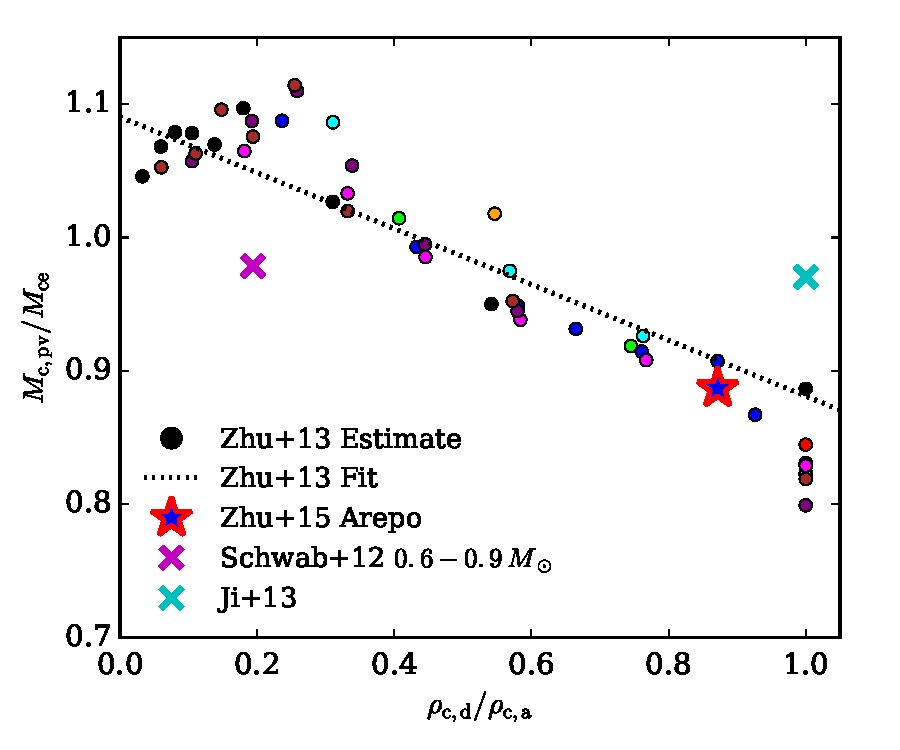
\includegraphics[angle=0,width=0.6\columnwidth]{chapter2_zhu+13/figures/c2a_McMce_vs_qrho.pdf}
\caption{Ratio of post-viscous degenerate core mass \Mcpv\ to remnant core-envelope mass \Mce\ (Sec. \ref{sssec:c2_masstrends}) as a function of \qrho\ for the systems of Ch. \ref{ch:ch2} (points), the $0.625 - 0.65\,\Msun$ remnant from the \arepo\ MHD simulation (red-blue star), the $0.6 - 0.6\,\Msun$ remnant of \citeauthor{ji+13} (\citeyear{ji+13}; cyan X) and the $0.6 - 0.9\,\Msun$ remnant of \citeauthor{schw+12} (\citeyear{schw+12}; magenta X).  The dotted line is a best fit to the Ch. \ref{ch:ch2} points given by Eqn. \ref{eq:c2a_mfit}.}
\label{fig:c2a_mcmce_qrho}
\end{figure}

In Fig. \ref{fig:c2a_mcmce_qrho}, we plot the ratio of \Mcpv\ to the core-envelope mass \Mce\ of the merger remnant (Sec. \ref{sssec:c2_masstrends}) as a function of \qrho, as well as a linear fit to the $\Mcpv/\Mce - \qrho$ relationship, 

\eqbegin
\frac{\Mcpv}{\Mce} = -0.21\qrho + 1.09
\label{eq:c2a_mfit}
\eqend

\noindent We use the $0.6 - 0.6\,\Msun$ remnant core mass ($1.1\,\Msun$) from \citealt{loreig09} for the \Mce\ of the \cite{ji+13}.  The core masses of the remnants used in \cite{schw+12} are not reported, so for their $0.6 - 0.9\,\Msun$ remnant (the sole system which overlaps with our parameter space) we substitute with our own \Mce.  Figs. \ref{fig:c2a_mcpvvsmtot} and \ref{fig:c2a_mcmce_qrho} show that, in all estimates of the viscous spin-down phase, a significant fraction of the total remnant mass is not accreted onto the core during viscous evolution.  For similar-mass mergers, both \cite{ji+13}'s simulation and our estimate suggest that the entire disk and a small amount of the core and envelope end up as a part of the hot envelope, leaving the core with slightly less mass than it had just after coalescence.  This runs counter to \citealt{vkercj10}'s assumption that the most of the disk will rapidly accrete onto the remnant, and explains why the increases in density and temperature during viscous evolution reported in this section are all a factor of a few smaller than that given in \citealt{vkercj10}.

%The $0.6 - 0.6\,\Msun$ remnant core mass from \citealt{loreig09} $\Mce$ for \citeauthor{ji+13}'s remnant

%\noindent (\Mcpv\ also has a weak inverse dependence on mass ratio \qm)
%and the amount of compressional heating the core experiences

%Our estimates' tendency to overestimate \Mcpv\ is likely because it assumes material not part of the remnant core is marginally bound with $E = 0$, leading to underestimation of the hot envelope mass.  Therefore our simple estimate overall does roughly produce the amount of mass remaining in the post-viscous core, and the amount of compressional heating the core experiences.(at least for dissimilar mass systems) attached to the degenerate core following spin down, but in detail tends to overestimate both effects.

For those systems that do not ignite nuclear fusion during the viscous phase, their next stage of evolution involves entropy being transported via neutrino cooling and radiative diffusion throughout and away from the remnant.  Since the remnant hot envelope ($\rho \lesssim 10^4\,\gcc$, $T \sim 10^9\,\mrm{K}$) is radiation-dominated, it has a near-Eddington luminosity, and thermal evolution will occur over a timescale \citep{shen+12}

\eqbegin
t_\mrm{therm} \sim E_\mrm{th, envelope}/L_\mrm{edd} \sim 10^4\,\mrm{yr}.
\eqend

\noindent (For those systems that do ignite fusion, the nuclear runaway time is $\lesssim10^2\,\mrm{yr}$, so this evolution will only occur to a very limited extent.)  \cite{shen+12} simulates this phase of thermal evolution using the \mesa\ \citep{paxt+11, paxt+13, paxt+15} stellar evolution code, starting with an artificial radial profile that approximates their $0.6-0.9\,\Msun$ post-viscous remnant.  Notably, they set the peak temperature at the base of the hot envelope (at $m \sim 0.9\,\Msun$) below the carbon ignition line.  They find the entropy from the remnant interior diffuses outward over $\sim10^4\,\mrm{yr}$, leading to the further compression and heating of the interior until carbon fusion ignites at the (non-degenerate) base of the envelope.  Meanwhile, convection rapidly redistributes entropy to much of the envelope, expanding it until its photosphere reaches $10^{12}-10^{13}\,\mrm{cm}$, comparable to giant stars.  They predict that their remnant will be converted into an ONe WD, much like in earlier calculations of near-Eddington accretion onto massive WDs (eg. \citealt{saion85}).

More recently, \cite{schw+16} have used \mesa\ to simulate the thermal evolution of their post-viscous $0.6-0.9\,\Msun$ remnant from \cite{schw+12}, and a more massive $0.64-0.96\,\Msun$ one from \cite{rask+14}.  The peak temperatures of both remnants are already high enough to ignite carbon nuclear fusion at the start; this generates a carbon-burning shell that propagates inward via conduction, reaching the center of the WD in $\sim2\times10^4\,\mrm{yr}$.  The result is a partly non-degenerate ONe proto-WD, which subsequently cools through neutrino losses and contracts.  For remnants with masses $\gtrsim1.35\,\Msun$, this leads to off-center \textit{oxygen-neon} burning to silicon-group elements, and for super-\Mch\ remnants, may even lead to fusion to iron followed by core-collapse into a neutron star.  For substantially sub-\Mch\ remnants that ignite non-explosive carbon burning, though, the likely end-result is a massive ONe WD.  The radiation-dominated envelope alongside the remnant's carbon-oxygen composition suggest that the remnant drives strong winds, complicating the thermal evolution and potentially leading to considerable mass loss \citep{shen+12, schw+16}.

%\cite{shen+12} simulate their $0.6-0.9\,\Msun$ remnant's thermal evolution in the \mesa\ \citep{paxt+11} 1D quasi-hydrostatic stellar evolution code.  Due to their viscous code using flattened cylindrical coordinates, they cannot directly port its output into \mesa, and instead evolve an artificial stellar profile that approximates the post-viscous remnant.  Notably, they set the peak temperature at the base of the hot envelope below the carbon ignition line.  They find the entropy from the remnant interior diffuses outward over $\sim10^4\,\mrm{yr}$, leading to the further compression and heating of the interior.  After $\sim6000\,\mrm{yr}$, carbon fusion ignites at the (non-degenerate) base of the envelope (at $m \sim 0.9\,\Msun$), though these values are of course dependent on their artificial initial conditions.  Whenever it is ignited, the nuclear burning zone will stably convert carbon into oxygen and neon, and will diffuse into the remnant interior over $10^4\,\mrm{yr}$.  Meanwhile, convection rapidly redistributes entropy to much of the envelope, expanding the envelope until its photosphere reaches $10^{12}-10^{13}\,\mrm{cm}$, comparable to giant stars.  

Thermal evolution of post-viscous remnants that are hottest at their \textit{center} have, to our knowledge, not yet been calculated.  We expect it would be qualitatively similar to what \cite{shen+12} and \cite{schw+16} found for their dissimilar-mass remnants: a further compression of the interior over $\sim10^4\,\mrm{yr}$, with compressional heating partially offset by radiative and neutrino cooling.  We thus expect that systems brought to the brink of ignition by viscous spin-down may subsequently ignite due to thermal contraction, though the number of such systems is likely small.  Those whose central temperatures are significantly below $6\times10^8\,\mrm{K}$ will cool too much during their compression to ignite; since neutrino cooling is density-dependent, they may experience off-center ignition instead.

%ch3
\chapter{Mergers in Smoothed-Particle and Moving Mesh Hydrodynamics}
\label{ch:ch3}

\begin{center}
\begin{minipage}[c]{4.75in}
Chenchong Zhu, R\"{u}diger Pakmor, Marten H. van Kerkwijk, Philip Chang\\
\vspace{2em}
\end{minipage}
\end{center}

The physics and final outcomes of the merger of two white dwarfs can currently only be directly studied in detail through 3D hydrodynamic simulations, and to date merger simulations have largely relied on smoothed-particle hydrodynamics, a method known to produce numerical artefacts under certain conditions.  In order to determine if the outcome of these simulations depend on the code being used, we followed the merger of a $0.625 - 0.65\,\Msun$ carbon-oxygen white dwarf binary in both the SPH code \gasoline\ and the moving mesh code \arepo.  We find that the two agree well with one another until the merger is complete.  Afterward, the merger remnant becomes axisymmetric over the course of a few hundred seconds in \gasoline, with most of its mass comprising a dense, oblate-spheroidal core.  The remnant in \arepo, on the other hand, remains non-axisymmetric and features a crescent-shaped core flanked on one side by a hot, underdense ``void''.  This configuration has an offset gravitational potential, which launches an $m = 1$ spiral mode within the surrounding disk that transports disk angular momentum over a timescale of $\sim10^3\,\mrm{s}$, substantially faster than suggested by other post-merger evolution studies.  These code-dependent differences could affect processes that occur early-on during post-merger viscous evolution.  The final product, of the merging process, however, likely remains a spherically symmetric dense core surrounded by a hot, non-degenerate envelope, regardless of which code is used.

%Since we performed our study, SPH codes, including \gasoline, have been updated to resolve many of their classic deficiencies, and a comparison with modern codes may yield different results.

\section{Introduction}
\label{sec:c3_intro}

%According to Loren-Aguilar et al. 2009, the very, very first WD simulations were made by Mochkovitch and Livio 1989 (1989A%26A...209..111M) using the self-consistent field method (SCF).  SCF isn't, as far as I can tell, time-dependent, so really they were just calculating the self-consistent structure of the merger remnant.  They do cite earlier RLOF work by Gingold and Monaghan 1979, but those simulations aren't of WD mergers per se.

Simulations of white dwarf (WD) mergers are a window into the detailed dynamics of the merging process and -- since mergers cannot directly be seen using current observational capabilities -- a link between observations of strange stars and explosive transients and theories about their formation.  Since the pioneering work of \cite{benz+90}, these simulations have overwhelmingly used a single numerical hydrodynamics implementation, smoothed-particle hydrodynamics (SPH).  Within SPH, regions of high density are automatically more resolved and advection is simulated without errors; its equations of motion also inherently conserve energy, linear and angular momentum.  These features make it attractive for modelling the bulk fluid flows and complicated geometry present in mergers.  Building on \citeauthor{benz+90} and other early works such as \cite{segrcm97} and \cite{guerig04}, more recent efforts have focused on more precise binary initial conditions \citep{dan+11}, exploration of remnant properties across parameter space (Ch. \ref{ch:ch2}; \citealt{loreig09, rask+12, dan+14}) and exploring the possible instigation and consequences of a nuclear explosion caused by the merger (eg. \citealt{pakm+10, dan+12, pakm+13, moll+14, rask+14}).

The traditional SPH formulation, however, is not without its problems (eg. \citealt{spri10,hopk15}): to be able to capture shocks, it uses an artificial viscosity, which can produce spurious heating and angular momentum transport in shear flows; it is known to suppress hydrodynamic instabilties; and captures shocks and steep gradients relatively poorly compared to other schemes at the same resolution.  Shocks, large-scale shear flows and the formation of instabilities are all expected for WD mergers, and comparisons between SPH and Eulerian grid codes for other astrophysical phenomena (eg. \citealt{dval+06, tracsp07, mitc+09}) have often shown qualitative and resolution-independent differences.  Reproducing simulations across different types of codes is essential both for development of numerical hydrodynamic schemes and for ensuring the physical validity of their results, and so we are motivated to simulate mergers with other hydrodynamic schemes.

%This suggests the need to simulate WD mergers with other hydrodynamics schemes.
%and incorrectly represent subsonic turbulence \citep{baues12}

A recent alternative to SPH, as well as Eulerian grid codes, is \arepo\ \citep{spri10}, one of a growing class of codes (eg. \citealt{duffm11, gabujl12, vandr16}) that render fluid evolution on a dynamically moving, unstructured mesh.  \arepo\ retains the accurate treatment of shocks and instabilities as well as negligible artificial viscosity that Eulerian grid codes feature, while gaining the automatic refinement and Galilean invariance inherent to SPH.  These features, coupled with a tree-based self-gravity solver, make it particularly attractive for astrophysical simulations (eg. \citealt{voge+12, pakms13, hayw+14, marips14, ohlm+16}), and, with the notable exception of formal angular momentum conservation, ideal for simulating WD mergers.  \cite{pakm+13} has already used \arepo\ to investigate initial mass transfer, and the possibility it sets off a helium detonation, in a 0.9 - 1.1 \Msun\ CO WD merger.

In this work, we compare the merger of a $0.625 - 0.65\,\Msun$ carbon-oxygen (CO) WD binary simulated in \arepo\ with one simulated in the SPH code \gasoline\ \citep{wadssq04}.  We generate identical initial conditions for both simulations, and disable chemical and nuclear evolution to focus solely on the hydrodynamic differences, aiming to learn whether critical hydrodynamic phenomena might have been missing or misrepresented in past SPH-based merger simulations.  Our results show that the two simulations closely resemble one another until the two WDs coalesce, after which the \gasoline\ merger remnant becomes axisymmetric over several hundred seconds, while the \arepo\ one remains asymmetric for much longer, potentially altering post-merger evolution.

%This work is also a companion to \citeauthor{zhu+15} (\citeyear{zhu+15}; henceforth \citeal{zhu+15}), which presents the growth of a seed magnetic field within the \arepo-based merger to amplitudes of $\sim10^{10}-10^{11}\,\mrm{G}$, which also has significant consequences for post-merger evolution.

In Section~\ref{sec:c3_codes}, we review the hydrodynamic schemes of SPH and \arepo, and discuss the parameters and initial conditions used in each simulation.  In Section~\ref{sec:c3_fixingarepo}, we summarize efforts to improve angular momentum conservation within \arepo.  In Section~\ref{sec:c3_results}, we present results for each code and compare their outcomes.  Lastly, in Sections~\ref{sec:c3_discussion} and \ref{sec:c3_conclusion}, we discuss which code represents the more physical result, and implications for mergers.

\section{Codes and Initial Conditions}
\label{sec:c3_codes}

All hydrodynamic and magnetohydrodynamic codes seek to properly evolve the continuum dynamics of a fluid on a discrete set of points in space and time.  Most astrophysical fluid codes (including the two we use) explore the simpler regimes of ideal hydro- or magnetohydrodynamics, where molecular viscosity and electrical resistance are negligible, as such is generally the case in astrophysical settings outside of planetary interiors.  The coupled partial differential equations of ideal magnetohydrodynamics, in their conservative form and with Gaussian units (eg. \citealt{goedp04, pakmbs11, pakms13, spru13}), is

%\citealt{feidc12} Sec. 3 is also useful; see also https://trac.princeton.edu/Athena/wiki/AthenaEqns for the full set of MHD equations.

\begin{eqnarray}
\ptl_t\rho + \ptl_j(\rho u^j) &=& 0 \nonumber \\
\ptl_t(\rho u^i) + \ptl_j(\rho u^iu^j + \delta^{ij}P_\mrm{tot} - \frac{1}{4\pi}B^iB^j) &=& -\rho \ptl^i\Phi \nonumber \\
\ptl_t(\rho e) + \ptl_j\left(u^j (\rho e + P_\mrm{tot}) - \frac{B^j}{4\pi}(u^lB_l)\right) &=& -\rho u^j\ptl_j\Phi \nonumber \\
\ptl_t B^i + \ptl_j(u^jB^i - u^iB^j) &=& 0,
\label{eqn:c3_mhd_eqns}
\end{eqnarray}

\noindent where $\rho$, $u^i$, $B^i$, and $\Phi$ are the density, velocity, magnetic field and gravitational potential, respectively, $P_\mathrm{tot} = P + \frac{1}{8\pi}B_jB^j$ is the total pressure, $e = \frac{1}{2}u_iu^i + e_\mathrm{int} + \frac{1}{8\pi\rho}B_jB^j$ is the specific total energy, and the usual Einstein summation convention holds.  This can be written in compact form:

\eqbegin
\frac{\ptl {\bf U}}{\ptl t} + \nabla\cdot{\bf F(U)} = {\bf G}
\label{eqn:c3_mhd_eqns_compact}
\eqend

\noindent where

\eqbegin
{\bf U} = 
\left( \begin{array}{c}
\rho \\
\rho {\bf u} \\
\rho e \\
{\bf B} \end{array} \right),
\label{eqn:c3_mhd_eqns_u}
\eqend

\eqbegin
{\bf F(U)} = 
\left( \begin{array}{c}
\rho {\bf u} \\
\rho {\bf u}{\bf u}^T + P_\mathrm{tot} - \frac{1}{4\pi}{\bf B}{\bf B}^T \\
{\bf u} (\rho e + P_\mathrm{tot}) - \frac{{\bf B}}{4\pi}({\bf u}\cdot{\bf B}) \\
{\bf B}{\bf u}^T - {\bf u}{\bf B}^T\end{array} \right),
\label{eqn:c3_mhd_eqns_fu}
\eqend

\eqbegin
{\bf G} = 
\left( \begin{array}{c}
0 \\
\rho {\bf g} \\
\rho {\bf u}\cdot {\bf g} \\
0 \end{array} \right)
\label{eqn:c3_mhd_eqns_g},
\eqend

\noindent and ${\bf g} = -\nabla\Phi$ is the gravitational acceleration.  Eqn. \ref{eqn:c3_mhd_eqns_compact} shows that the time-derivative of the fluid's values is given by the sum of a flux term (since, by the Green-Gauss theorem, the integral of $\nabla\cdot{\bf F(U)}$ within a volume is equivalent to a flux across its boundary) and a (self-)gravitational source term ${\bf G}$.  These are generally calculated separately, and then combined.

To better understand the code comparison in this chapter, and to preface the discussion of improving \arepo's angular momentum conservation in Sec. \ref{sec:c3_fixingarepo}, we present an extremely short and semi-qualitative discussion of how these equations are implemented within SPH and \arepo.  The historical development of both methods is long and involved, and, as improving hydrodynamic schemes is not the focus of this thesis, we will refer the reader to the review articles referenced throughout this section for further details.

\subsection{Traditional Smoothed-Particle Hydrodynamics}
\label{ssec:c3_sph}

SPH, first introduced in \cite{lucy77} and \cite{gingm77}, is a mature simulation method used in a host of astrophysical contexts ranging from star formation to cosmology.  Our overview summarizes the first few sections of \citep{spri10rev}; we also refer readers to \cite{mona05}, \cite{ross09} and \cite{pric12} for further details.

SPH represents a fluid with a set of particles.  The fluid's continuum properties at some point ${\bf r}$ in the simulation are sampled by using these particles as interpolation points.  Representing any given continuum property (the most important of which is density, since it factors into the equations of motion) as $F({\bf r})$, we can use a ``kernel'' $W({\bf r}, h)$ to generate its approximate, locally-averaged value

\eqbegin
F_s({\bf r}) = \int F({\bf r'})W({\bf r} - {\bf r'}, h)d{\bf r'}.
\eqend

\noindent In the (computationally impossible) case of infinite resolution, we can choose $W({\bf r}, h)$ to be a Dirac delta, and $F_s({\bf r}) = F({\bf r})$, but in practice we choose $W({\bf r}, h)$ to extend over some characteristic ``smoothing length'' $h$.  If $W({\bf r}, h)$ were a Gaussian, $h = \sigma$, the standard deviation.  The most popular form of $W({\bf r}, h)$ is a cubic spline that goes to zero when ${\bf r} > 2h$, and $h$ is generally set to ensure a user-defined number of neighboring particles $N$ fall within the kernel.  For a set of particles with associated mass $m_i$ and known values of $F_i = F({\bf r}_i)$, we can discretize the integral as

\eqbegin
F_s({\bf r}) \simeq \sum_j\frac{m_j}{\rho_j}F_j W({\bf r} - {\bf r}_j, h).
\label{eq:c3_kernelavg}
\eqend

\noindent where $\rho_i$ can be estimated using 

\eqbegin
\rho_i \simeq \sum_j m_j W({\bf r}_i - {\bf r}_j, h)
\label{eq:c3_kernelavg_rho}
\eqend

\noindent Derivatives of the field can also be determined using the gradient of the kernel $\nabla_i W_{ij}$.

Meanwhile, the Euler equations (Eqn. \ref{eqn:c3_mhd_eqns_compact} without the gravitational and magnetic terms) can be shown to follow the Lagrangian:

\eqbegin
L = \int \rho\left(\frac{{\bf u}^2}{2} - e\right)dV
\label{eqn:c3_lagrangian}
\eqend

\noindent which can be discretized for a set of particles as

\eqbegin
L_\mathrm{SPH} = \sum_i \frac{1}{2}m_i {\bf u_i}^2 - m_i e_i.
\eqend

\noindent This suggests a time-evolution scheme for the fluid.  Each particle representing the fluid is given a (time-independent) mass $m_i$, position ${\bf r}_i$, velocity ${\bf u}_i$ and specific internal energy $e_i$; the fluid can then be simulated by time-evolving the latter three terms for all particles.  The equations governing ${\bf u}_i$ and $e_i$ are derived by applying the Euler-Lagrange equation ($\frac{d}{dt}\frac{\ptl L}{\ptl \dot{{\bf r}}_i} - \frac{\ptl L}{\ptl {\bf r}_i} = 0$) to $L_\mathrm{SPH}$.  They traditionally take the form:\footnote{We state \cite{wadssq04}'s formulation of Eqns. \ref{eqn:c3_spheqnm} and \ref{eqn:c3_spheqne}, as \cite{spri10rev} assumes a different method of controlling the smoothing length $h_i$.}

\eqbegin
\frac{d{\bf u}_i}{dt} = -\sum_j m_j\left(\frac{P_i}{\rho_i^2} + \frac{P_j}{\rho_j^2} \right)\nabla_i W_{ij}
\label{eqn:c3_spheqnm}
\eqend

\eqbegin
\frac{d e_i}{dt} = \frac{P_i}{\rho_i^2}\sum_j m_j\left({\bf u}_{i} - {\bf u}_{j}\right)\cdot\nabla_i W_{ij}
\label{eqn:c3_spheqne}
\eqend

\noindent where pressure $P_i$ is determined from $\rho_i$ and $e_i$ using a user-prescribed equation of state.  The left panel of Fig. \ref{fig:c3_codediag} summarizes this scheme.  Note that since Eqn. \ref{eqn:c3_lagrangian} has no time-dependence and is translationally and rotationally invariant, SPH naturally conserves total energy, momentum and angular momentum.  Self-gravity can be added as an additional force to Eqn. \ref{eqn:c3_spheqnm} (see \citealt{spri10rev}, Sec. 2.4, and \citealt{wadssq04}, Sec. 2.1) using methods originally developed for $N$-body simulations.  Magnetic fields can also be included (eg. \citealt{pric12, lewibt16}), but the resulting ``SPMHD'' formulation is not used in this thesis.

% Eqn. \ref{eqn:c3_spheqne} can actually be replaced with $d s_i/dt = 0$, except in the presence of shocks

%(as the differential form of the Euler equations breaks down across a shock front)

As given, the SPH equations of motion conserve entropy, but entropy must increase in the presence of shocks.  The most popular solution is to add an artificial viscosity term

\eqbegin
-\sum_j m_j \Pi_{ij} \nabla_i W_{ij}
\eqend

\noindent to Eqn. \ref{eqn:c3_spheqnm}, where, defining ${\bf r}_{ij} = {\bf r}_i - {\bf r}_j$ and ${\bf u}_{ij} = {\bf u}_i - {\bf u}_j$,

\eqbegin
\Pi_{ij} =
    \begin{cases}
      \frac{-\alpha\frac{1}{2}(c_i + c_j)\mu_{ij} + \beta\mu_{ij}^2}{\frac{1}{2}(\rho_i + \rho_j)} & \mrm{for\,} {\bf u}_{ij}\cdot{\bf r}_{ij} < 0 \\
      0 & \mrm{otherwise},
    \end{cases}
\label{eq:c3_artificialvisc}
\eqend

\noindent where $\mu_{ij} = \bar{h}{\bf u}_{ij}\cdot{\bf r}_{ij}/(|{\bf r}_{ij}|^2 + 0.04\bar{h}^2)$, $\bar{h} = \frac{1}{2}(h_i + h_j)$, $c_i$ is the sound speed and $\alpha$ and $\beta$ are tunable parameters ($\beta = 2\alpha$ is used in \gasoline).  In addition to facilitating shock capture, $\Pi_{ij}$ also prevents spurious particle interpenetration between interacting flows \citep{hernk89}.  It, however, can also introduce spurious viscous forces, and so must be damped in the absence of shocks.  In shear flows, this can be done with a ``Balsara switch'', which multiplies $\Pi_{ij}$ with a prefactor, proportional to the ratio between the divergence and curl of velocity, that goes to zero in the presence of a pure shear flow.  It is also possible to make the $\alpha$ and $\beta$ coefficients in $\Pi_{ij}$ time-variable (eg. \citealt{morrm97, dola+05}) with

\eqbegin
\frac{d\alpha_i}{dt} = -\frac{\alpha_i - \alpha_\mrm{min}}{\tau_i} + S_i
\label{eq:c3_timevariablealpha}
\eqend

\noindent where $\tau_i = h_i/(c_i l)$, $l$ is a tunable parameter of order unity, $S_i$ is a source term that becomes large in the presence of shocks, and $\alpha_\mrm{min} > 0$ is a minimum $\alpha$ value to negate noise and spurious particle interpenetration in smooth flows.  Eqn. \ref{eq:c3_timevariablealpha} exponentially damps $\alpha_i$ to its minimum value over timescale $\tau_i$ in the absence of shocks, and increases it via the source term when shocks are present.  Both these methods are used in \gasoline.

%{eq:c3_artificialvisc}

As explained in the introduction, SPH's Lagrangian nature allows it to automatically resolve regions of high density, simulate advection without errors, and conserve energy, linear and angular momentum to high accuracy.  These features make it much easier to model mergers in SPH than in Eulerian grid schemes, which discretize the simulation volume on a static grid, and time-evolve the system by tracking fluid fluxes between grid cells.  These traditionally have issues with simulating advection and adaptively increasing the spatial resolution ahead of moving fluids, such as orbiting binary stars, except under specific coordinate systems and symmetries.  Thus, they have rarely been used to simulate WD mergers (see \cite{katz+16} for recent developments).

The limitations of SPH (and Eulerian codes) have also been well-covered in literature (see, eg., the introductions to \citealt{spri10, hopk15, katz+16}).  Chief among them is the artificial viscosity discussed above, which can produce spurious heating and angular momentum transport in shear flows even in codes that utilize the Balsara switch and time-variable viscosity \citep{culld10}.  Classical formulations of SPH have also been known to suppress hydrodynamic instabilities (eg. \citealt{ager+07}) due to poor treatment of contact discontinuities manifesting as a ``surface tension'' (eg. \citealt{readha10, hesss10}).  While this has subsequently been resolved (eg. \citealt{hopk13, hu+14, kell+14}) by introducing artificial mixing terms \citep{pric08} and smoothing the pressure as well as the density across discontinuities (eg. by replacing the $P_i/\rho_i^2 + P_j/\rho_j^2$ term in Eqn. \ref{eqn:c3_spheqnm} with $(P_i + P_j)/(\rho_i\rho_j)$; \citealt{kell+14}) the vast majority of merger simulations in the literature come from before these alterations became widely used.  SPH resolves shocks and steep gradients relatively poorly compared to Eulerian schemes due to kernel smoothing of the density, and can corrupt smooth flows with particle velocity noise \citep{spri10rev}.  Lastly, SPH particles naturally tend toward a locally isotropic and regular configuration \citep{pric12}, and in physical systems where they are irregularly distributed, such as in shear flows and in shocked material, Eqn. \ref{eqn:c3_spheqnm} produces spurious forces to restore regularity (eg. \citealt{readha10, dehna12}).  In some situations, this resolution-independent ``$E_0$ error'' produces enough noise to drown out large-scale structures \citep{hopk15}.  All of these issues motivate both the further development of SPH and competing hydrodynamic schemes, and simulating mergers in a diversity of codes.

%the E0 error also contributes to poor treatment of discontinuities; 

\subsection{GASOLINE SPH Code}
\label{ssec:c3_gasoline}

\gasoline\ is a modular, tree-based SPH code that we previously used to explore the parameter space of CO WD mergers in Ch. \ref{ch:ch2}.  Code settings and initial conditions used in this work are nearly identical to those used in Ch. \ref{ch:ch2}.  We utilize \gasoline's default \cite{hernk89} kernel with 100 neighbors, and use the asymmetric energy formulation (\citeauthor{wadssq04} Eqn. 8) to evolve particle internal energy.  Artificial viscosity is dynamically controlled using a combination of the Balsara switch and time-variable coefficients for the $\alpha$ and $\beta$ viscosity terms ($\alpha\,=0.05$, $\beta\,=0.1$ when shocks are not present, and approximately unity when they are).  We utilize the Helmholtz equation of state (EOS; \citealt{timms00}) to properly represent arbitrarily degenerate and relativistic gases.  Since \gasoline\ tracks the particle internal energy, while Helmholtz uses temperature as an input, a Newton-Raphson inverter is included in the EOS to determine the latter from the former.  Helmholtz includes analytic expressions for Coulomb corrections that lead to negative entropy values for cold and dense material (eg. $T\lesssim10^6\,\mrm{K}$ when $\rho\sim10^7\,\gcc$).  When this occurs, the EOS sets all Coulomb contributions to zero, but this produces a jump in the pressure and internal energy of order $1$\%, which can cause the Newton-Raphson inverter to fail.  To keep the energy-temperature relation monotonic for the inverter, we enable Coulomb corrections even when the total entropy becomes negative.  SPH noise occasionally brings highly degenerate particles to below the Fermi energy.  Under these conditions we set the pressure to the Fermi pressure, but let the energy freely evolve (see Sec. \ref{ssec:c2_sphcode}).

Like in our previous work, we ignore outer hydrogen and helium layers, composition gradients, and any nuclear reactions, in order to focus on the merger hydrodynamics.  Previous work that did include nuclear reactions (\citeal{loreig09}; \citealt{dan+12}), and in one case an outer helium layer \citep{rask+12}, have shown that they play a negligible role in the hydrodynamics of a $0.625 - 0.65\,\Msun$ CO WD merger.  More massive binaries, as well as less massive ones involving a CO-He hybrid WD, may experience He or CO detonations during the merger \citep{pakm+10, rask+12, dan+12, pakm+13}.

We use the same version of \gasoline\ as in Ch. \ref{ch:ch2}, which does not include the improvements recently introduced in \textsc{Gasoline2} \citep{kell+15, tamb+15} and \textsc{ChaNGa/Gasoline} \citep{gove+15}.  These include a turbulent diffusion scheme to facilitate fluid mixing \citep{shen+10} and the use of the $(P_i + P_j)/(\rho_i\rho_j)$ density-averaged pressure term in the SPH force expression \citep{kell+14} to properly treat contact discontinuities.  We also do not consider more advanced prescriptions for viscosity, such as Godunov-SPH (eg. \citealt{chaw16}), as these are generally not implemented in SPH codes.  We again stress that the purpose of this work is to compare the traditional SPH formulation, used in almost all merger simulations to date, to \arepo, and we leave comparisons with improved and modified SPH schemes to future work.

%kell+14 is practically equivalent to the pressure-entropy formulation of \cite{hopk13})

\subsection{AREPO Moving Mesh Code}
\label{ssec:c3_arepo}

\begin{figure}
\centering
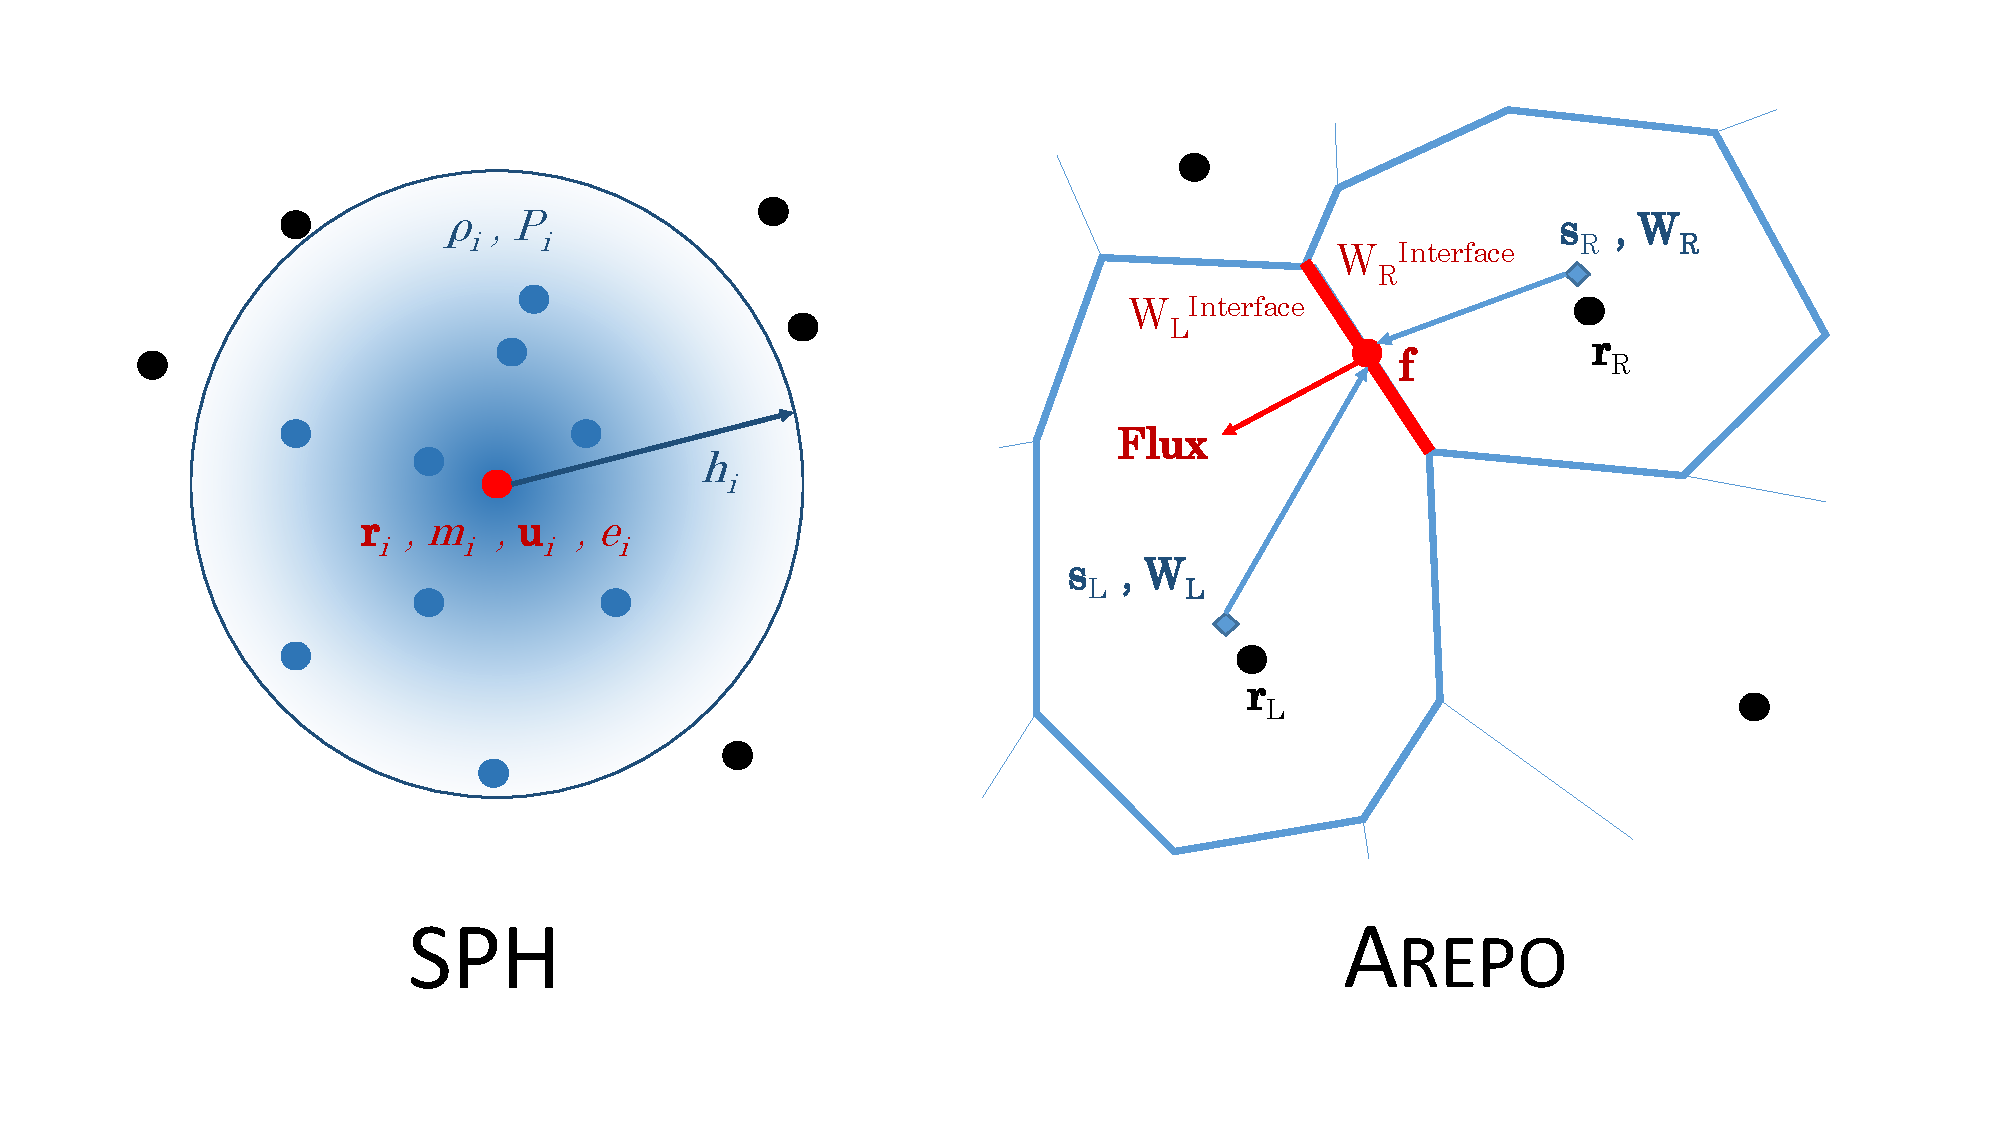
\includegraphics[angle=0,width=1.0\columnwidth]{chapter3_zhu+u/figures/SPHArepoFig.pdf}
\caption{Schematics for the SPH and \arepo\ hydrodynamic schemes.  In SPH (left), the fluid is discretized into particles, each of which possesses a position ${\bf r}_i$, mass $m_i$, velocity ${\bf u}_i$ and specific internal energy $e_i$.  The density $\rho_i$ of a given particle (red point) is determined by kernel sampling its neighbors (blue) within a smoothing length $h_i$ (Eqn. \ref{eq:c3_kernelavg_rho}); pressure $P_i$ is then obtained using the density and internal energy.  The particle is evolved by kernel sampling nearby pressures and densities, and applying the SPH equations of motion (Eqns. \ref{eqn:c3_spheqnm} and \ref{eqn:c3_spheqne}).  In \arepo\ (right), the fluid is discretized using an unstructured mesh defined by Voronoi tessellation.  Each Voronoi cell possesses a mesh-generating point ${\bf r}_i$ and a set of conserved quantities equivalent to ``primitive variables'' ${\bf W}_i = \left(\rho_i, {\bf u}_i, P_i, {\bf B}_i\right)$, i.e. the values of density, velocity, pressure and magnetic field amplitude at the cell's center of mass ${\bf s}_i$.  Note that ${\bf r}_i \neq {\bf s}_i$, but their separation is typically a few percent of the cell's radius, and has been exaggerated above.  Fluxes between two cells $\mrm{L}$ and $\mrm{R}$ are calculated by propagating their primitive variables ${\bf W}_\mrm{L,R}$ to the centroid of their interface ${\bf f}$ to obtain ${\bf W}_\mrm{L,R}^\mrm{interface}$ (Eqn. \ref{eq:c3_muscl_hancock}, or Eqn. \ref{eq:c3_rk2_timeevo} following \citealt{pakm+16}), and then solving the Riemann problem (in the frame of the interface).  The mesh is evolved by moving the mesh generating points ${\bf r}_i$ at roughly the fluid velocity ${\bf u}_i$, calculating fluxes between all cells, and then updating each cell's conserved quantities.  While evolving an SPH particle requires the use of dozens of its neighbors for kernel averaging, evolving an \arepo\ cell only requires those neighbors directly adjacent to it.}
\label{fig:c3_codediag}
\end{figure}

We now introduce \arepo's moving-mesh magnetohydrodynamics scheme, summarizing \cite{spri10}, \cite{pakmbs11} and \cite{pakms13}.  \arepo\ discretizes a fluid using a mesh (i.e. a grid), much like static Eulerian codes.  To overcome the traditional Eulerian code shortcomings of not being Galilean invariant, having large advection errors and having difficulty adjusting spatial resolution for complex flows, \arepo\ moves the mesh to follow local fluid motion.  Fluxes between mesh cells are calculated in the frame of the (moving) cell walls that divide them -- this preferred frame choice, in addition to the moving mesh, give the scheme a Lagrangian nature and automatic spatial refinement similar to SPH.  Allowing a structured grid to move with the fluid can lead to severe mesh deformation that prevent its further evolution.  \arepo\ circumvents this by utilizing an unstructured mesh defined by Voronoi tessellation of a set of ``mesh-generating points'', each of which corresponds to a single mesh cell (see \citealt{spri10}, Sec. 2).  The mesh-generating points are given the velocities of the fluid they represent, and the tessellation is redone at each timestep.  The result is a moving mesh that, due to the mathematical properties of Voronoi tessellation, does not suffer from mesh-tangling effects.  To keep the Voronoi mesh regular (improving computational efficiency), mesh-generating point velocities are slightly altered from their pure Lagrangian values, and additional velocity adjustments can be made to keep cells near a constant mass or volume.  This representation of the fluid also couples more naturally to $N$-body based gravity solvers (see \citealt{spri10}, Sec. 3), with \arepo\ using a nearly identical TreePM solver as the SPH code \textsc{gadget2} \citep{spri05}.

%The mesh is constructed by Voronoi tesselation of a set of mesh generating points, and these points are given velocities to follow local fluid motion in a Lagrangian fashion.  This results in a mesh that deforms over time to track the evolution of the fluid, without the mesh-tangling effects that hindered previous moving mesh schemes.  Mesh generating point velocities are slightly altered from their pure Lagrangian values to keep the Voronoi mesh regular, reducing flux calculation errors.  Additional velocity adjustments can be made to keep cells near a constant mass or volume, but in practice this becomes ineffective for highly non-linear flows.  Fluid fluxes between cells are calculated using a second-order Godunov scheme with an exact Riemann solver (in our case HLLD), while self-gravity is handled using a TreePM solver, nearly identical to the one used by SPH code \textsc{gadget2} \citep{spri05}.

On the Voronoi mesh, \arepo\ tracks the finite volume integral of ${\bf U}$ (Eqn. \ref{eqn:c3_mhd_eqns_u}) for each cell, i.e. 

\eqbegin
{\bf Q}_i = \int_{V_i} {\bf U}dV = \left( \begin{array}{c}
m_i \\
{\bf p}_i \\
E_i \\
{\bf B}_i V_i \end{array} \right),
\eqend

\noindent where $m_i$ is the cell mass, ${\bf p}_i$ its momentum, $E_i$ its total energy and ${\bf B}_i V_i$ the magnetic field multiplied by the cell volume.  The time-evolution for cell $i$ from timestep $n$ to $n+1$ is then given by

\eqbegin
{\bf Q}_i^{n+1} = {\bf Q}_i^n - \Delta t\sum_j A_{ij} {\bf \hat{F}}_{ij}^{n + 1/2}
\label{eq:c3_arepo_timeadv}
\eqend

\noindent where $\Delta t$ is the timestep, $j$ stands for all cells that border cell $i$, $A_{ij}$ is the oriented area of the face dividing cells $i$ and $j$ and ${\bf \hat{F}}_{ij}$ is the estimated flux between them (positive flux means escaping from $i$).  In practice fluxes are more easily calculated using primitive variables 

% They're more easily calculated because of the Galilean transforms needed to determine cell fluxes, and to make self-gravity easier to calculate.

\eqbegin
{\bf W}_i = \left( \begin{array}{c}
\rho_i \\
{\bf u}_i \\
P_i \\
{\bf B}_i \end{array} \right)
\eqend

%(then boosted back into the simulation frame of reference) to maintain Galilean invariance.  This means that each hydrodynamic step first calculates the Voronoi mesh and assigns velocities ${\bf w}_i$ to the mesh-generating points before calculating $W$ and ${\bf \hat{F}}$ and then advancing time using Eqn. \ref{eq:c3_arepo_timeadv} (\citealt{spri10}, Sec. 3).  Under standard \arepo\ operation, ${\bf w}_i$ is the same as cell fluid speed ${\bf v_i}$, with a small corrective term to keep the mesh regular, but ${\bf w}_i$ could also be set to zero, turning \arepo\ into a static unstructured-grid code.  Once the velocities are set, the flux across $A_{ij}$ can be determined from the (boosted) primitive values at either side -- which we term the ``left'' and ``right'' states, respectively -- of the face's centroid.  

\noindent and then converted back to ${\bf Q}$.  As noted earlier, fluxes are calculated in the frame of face $A_{ij}$ to maintain Galilean invariance, so ${\bf W}$ on either side of the face -- which we term the ``left'' and ``right'' cells -- are boosted by $A_{ij}$'s velocity before being used.  The geometry of this setup can be seen in the right panel of Fig. \ref{fig:c3_codediag}. In \arepo's original formulation \citep{spri10}, the values of ${\bf W}^\mrm{interface}$ on the left and right sides of $A_{ij}$'s centroid are determined from their respective cell's ${\bf W}$ using the MUSCL-Hancock (eg. \citealt{vlee06}; MUSCL stands for ``Monotonic Upstream-Centered Scheme for Conservation Laws'')  approach of a piecewise linear spatial reconstruction and a first-order time-extrapolation by half a timestep:

\eqbegin
{\bf W}_\mrm{L,R}^\mrm{interface} = {\bf W}_\mrm{L,R} + {\bf \frac{\partial W}{\partial r}}\Bigr|_\mrm{L,R}({\bf f} - {\bf s}_\mrm{L,R}) + {\bf \frac{\partial W}{\partial t}}\Bigr|_\mrm{L,R}\frac{\Delta t}{2},
\label{eq:c3_muscl_hancock}
\eqend

\noindent where ${\bf f}$ is the position of $A_{ij}$'s centroid, and ${\bf s}$ each cell's center of mass.  We note that the cell center of mass is not identical to the cell's mesh generating point position ${\bf r}$ (Fig. \ref{fig:c3_codediag}), but is generally a few percent the radius of the cell.  The spatial gradient is estimated by taking advantage of the Green-Gauss theorem.  Given some scalar field $\phi$, its gradient is given by

\eqbegin
\left\langle \nabla \phi \right\rangle_i \simeq -\frac{1}{V_i} \sum_j \phi({\bf f}_{ij}){\bf A_{ij}}.
\label{eq:c3_gauss_green}
\eqend

\noindent $\phi({\bf f}_{ij})$ is $\phi$ at $A_{ij}$'s centroid, and can be estimated by appealing to the geometric properties of Voronoi cells (see \cite{spri10}, Sec 3.1).  The temporal gradient is determined by relating it to the spatial gradient using the Euler equations.  Finally, the flux is resolved from ${\bf W}_\mrm{L,R}^\mrm{interface}$ with a Riemann solver (in all our simulations, the Harten-Lax-van Leer -- Discontinuities, or HLLD, solver; \citealt{miyok05}).  Eqns. \ref{eq:c3_muscl_hancock} and \ref{eq:c3_gauss_green} were replaced in \cite{pakm+16} order to resolve \arepo's angular momentum conservation issue (Sec. \ref{sec:c3_fixingarepo}), but the overall flux calculation procedure remains the same as above.

%Once calculated, the gradient estimate is slope-limited before being used in Eqn. \ref{eq:c3_muscl_hancock} (\cite{spri10} Eqns. 28 - 30)

The self-gravity term ${\bf G}$ from Eqn. \ref{eqn:c3_mhd_eqns_compact} can easily be added to the flux calculation, since, when using ${\bf W}$, gravity only changes the momentum.  This change, and the corresponding one for kinetic energy, can then be appended to ${\bf Q}$ (\citealt{spri10}, Sec. 5.2).  

%The advantages of \arepo\ -- automatic adaptive resolution enhancement, Galilean invariance, accurate shock capture, low velocity noise and artificial viscosity in smooth flows, and a natural coupling to particle-based gravity solvers -- make it an excellent platform with which to simulate mergers.

For the simulations in this chapter, we set ${\bf B} = 0$, reducing \arepo\ to a purely hydrodynamic simulation (Ch. \ref{ch:ch4} considers the MHD case).  We use the same Helmholtz EOS in \arepo\ that we installed into \gasoline\ and also ignore composition gradients and any nuclear reactions.  To assure reasonably constant mass and volume resolutions, we use an explicit refinement scheme \citep{voge+12} that adds or subtracts mesh-generating points to the grid.  

%This keeps cell masses near a fixed value, and keeps all cell volumes within one order of magnitude of each other.

\subsection{Initial Conditions and Completion Time}
\label{ssec:c3_initcond}

Our chosen WD masses are typical of the narrowly peaked empirical mass distribution of field CO WDs \citep{tremb09, klei+13}.  As in Ch. \ref{ch:ch2}, we generated WDs by rescaling a sphere of particles to the proper enclosed mass-radius relation determined from 1D hydrostatic integration.  We used a 50\% C, 50\% O composition by mass uniform throughout the star, and assumed a uniform temperature of $5\times 10^6$ K.  The stars were placed into \gasoline\ for approximately 11 dynamical times (33.3 s for the $0.625\,\Msun$ WD and 31.3 s for the $0.65\,\Msun$ WD).  Thermal energy and particle velocity were damped to $\sim 5 \times 10^6$ K and 0 cm s$^{-1}$ during the first dynamical time, and left free during the remaining 10.  64 neighbors, rather than 100, were used during relaxation to minimize the number of particle pairs generated.  These pairs (ex. \citealt{dehna12}, \citealt{spri10rev}) do not change global properties of the relaxed WDs, but do effectively reduce spatial resolution and having too many of them make transferring SPH initial conditions into \arepo\ problematic.  Following relaxation, the density profile of both stars were consistent with the hydrostatic equilibrium solution, with the numerical central densities deviating from the 1D integrated ones by less than 1\%.  Since all particles have identical mass, the tenuous outer layers of the WDs are difficult to capture in \gasoline; consequently the radii of the relaxed stars, as defined by the outermost particle, were $\sim 5$\% smaller than the integrated ones.  Even after energy damping, particle noise prevents the central temperature of the relaxed stars from reaching below $\sim 1\times 10^7$ K, so all particle temperatures were artificially reset to $\sim 5 \times 10^6$ K.

We then placed the relaxed stars in a circular, unsynchronized binary, with initial separation $\azero = 2.2\times10^9\,\mrm{cm}$ chosen (using the approximation of \citealt{eggl83}) so that the $0.625\,\Msun$ donor just overflows its Roche lobe.\footnote{The 1D integrated radius was used to calculate \azero, rather than the smaller relaxed SPH radius.  This accounts for the small differences in initial conditions between this work and the equivalent simulation in Ch. \ref{ch:ch2}.}  The corresponding orbital period is $49.5\,\mrm{s}$.  These initial conditions do not account for the tidal bulges of the stars, and so are not fully equilibrated (eg. \citealt{dan+11}).  While this makes our initial conditions less realistic, it should suffice for our purpose of discovering any code dependence on merger evolution.

We generate initial conditions in \arepo\ by converting the SPH particles of the \gasoline\ initial conditions into mesh-generating points, while retaining their conserved quantities (mass, momentum and energy).  These initial conditions are not guaranteed to be regular, but \arepo\ regularizes the mesh over just a few timesteps by nudging each cell's mesh-generating points to their cell's center of mass.

%Factor of 2 - 3 in resolution comes from gasoline needing 100 neighbors, so its resolution R is given by 100V = 4/3piR^3 -> R = 2.88V^1/3 , while arepo has R = V^1/3, where V is the characteristic volume for a single point.  Gasoline technically has a better resolution than that, since a cubic spline kernel counts nearby particles more highly, but there's some ambiguity in comparing between the two codes (for example, should R = 0.5V^1/3 for arepo?)

Our SPH particles all have the same mass of $2\times10^{27}\,\mrm{g}$ ($1.3\times10^{6}$ particles represent the system), comparable to the highest resolutions used in other recent work \citep{pakm+12, rask+14}.  We likewise use \arepo's refinement scheme to keep cell masses within a factor of $2$ of this value, and to keep adjacent cell volumes to within a relative factor of 10.  \arepo's grid refinement scheme naturally increases the resolution of our simulations over time, though, and so all resolutions stated in this work are for the start of the simulation.  We additionally initialize a background grid of $10^{-5}\,\gcc$ cells in \arepo\ to fill the vacuum surrounding the WDs -- this adds only $\sim0.005\,\Msun$ of material to the simulation.  At identical mass resolution, the spatial resolution in \gasoline\ is about a factor of $2-3$ lower than that in \arepo\ due to \gasoline's use of more neighboring particles to obtain smoothed quantities.  The two codes differ greatly regardless of resolution, however, and we believe equivalent mass resolution to be the most appropriate comparison (see \citeauthor{voge+12} Sec. 2.3 for complications in achieving equivalent accuracy in SPH and grid codes).  In Sec. \ref{ssec:c3_restest} we check if our results are resolution-dependent.

We run both simulations to $1000\,\mrm{s}$, substantially beyond the time when the WDs merge (at $\sim200\,\mrm{s}$).  At this point, the \gasoline\ simulation has reached a quasi-hydrostatic equilibrium.  As we shall see in Sec. \ref{sec:c3_results}, the \arepo\ simulation continues its hydrodynamic evolution long after this time.

% it begins a phase of slow secular spin-down due to artificial viscosity redistributing angular momentum  ydrodynamic evolution has also ended for the \arepo\ simulation by $\sim400\,\mrm{s}$, and the merger remnant also subsequently evolves much more slowly, 

%our two high resolution runs to a \gasoline\ run with $1\times10^{28}\,\mrm{g}$ particle mass, comparable to those used in parameter-space sweeps \citep{dan+12, zhu+13, dan+14}, and an \arepo\ simulation with the same target cell mass.

\section{Improving Angular Momentum Conservation in Arepo}
\label{sec:c3_fixingarepo}

Before we describe our results, we summarize the discovery and resolution of a critical angular momentum conservation issue in \arepo.

% DON'T WRITE THIS: in your 2013 simulations the initial binary separation wasn't consistent for initial conditions.  As a result, coalescence times tend to be slightly longer
% In your 2014 NoVolRef production runs you solved this problem.  At that point Arepo was disrupting earlier, but since you don't use those runs anywhere in the chapter, you shouldn't mention these times.
% In it, the $0.625\,\Msun$ donor WD was destroyed by tidal forces within $\sim2.6$ orbital periods ($\sim130\,\mrm{s}$), versus the \gasoline\ simulation's $\sim3.7$ ($\sim180\,\mrm{s}$).  

The first simulation we performed in \arepo\ showed dramatic differences from our \gasoline\ ones.  Following the final phase of the merger, when the two WDs coalesce into one, the \arepo\ merger remnant featured a dense, crescent-shaped region formed from accretor material that retained its pre-merger temperature of $\lesssim10^7\,\mrm{K}$, while the \gasoline\ remnant was relatively hot throughout its interior, with an average temperature of $\sim2\times10^8\,\mrm{K}$.  Most prominently, the \gasoline\ one became axisymmetric within several hundred seconds after the merger, while the \arepo\ remnant maintained the integrity of its non-axisymmetric crescent while launching one, and then multiple trailing spiral waves into the surrounding medium.

%and in this section we summarize our attempts at isolating the cause of this angular momentum leak, and which features discussed above turned out to be spurious once the leak was plugged.

\begin{figure}
\centering
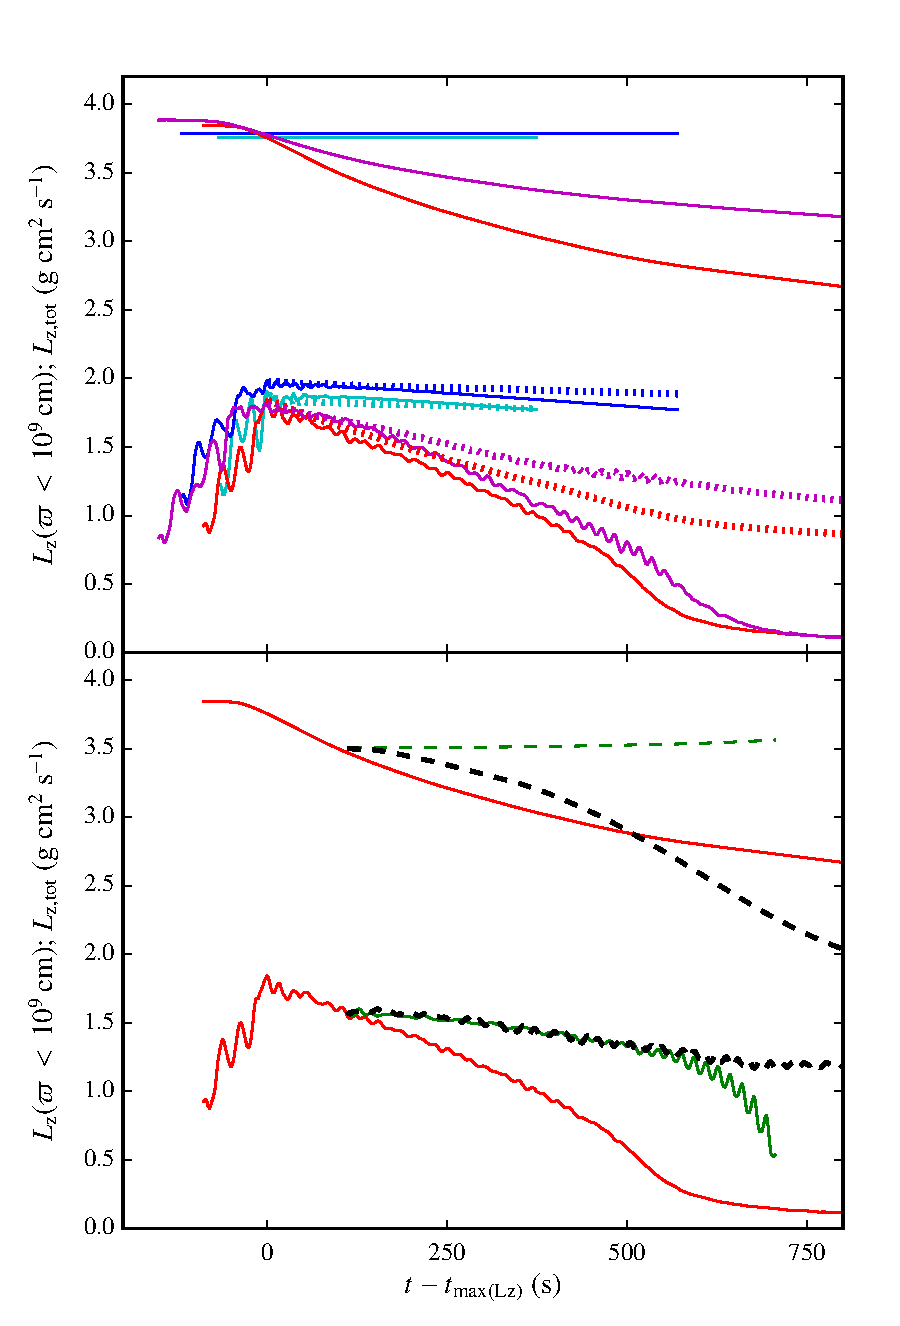
\includegraphics[angle=0,width=0.6\columnwidth]{chapter3_zhu+u/figures/lz_development.pdf}
\caption{Evolution of total $z$-axis angular momentum \Lztot\ (top cluster of lines in each panel) and that within a cylinder of radius $\varpi = 10^9\,\mrm{cm}$, \Lzinner\ (bottom cluster), for various simulations in 2013-2014, before \arepo\ was updated to better conserve angular momentum.  All curves are shifted in time by \tlm, the time in each simulation at which \Lzinner\ achieved its maximum value, to synchronize the start of post-merger evolution.  In the top panel, red and magenta lines represent the low and standard-resolution \arepo\ simulations, respectively, while the cyan and blue ones represents low and standard-resolution \gasoline\ ones, respectively.  Dotted lines represent angular momentum balance $\Lbal(\winnercyl)$, which should be flat in the absence of spurious angular momentum losses.  (Slightly different initial amounts of total angular momentum between \arepo\ and \gasoline\ runs are due to inconsistencies in their initial conditions that have subsequently been eliminated.)  In the bottom panel, the red line is again the low-resolution \arepo\ simulation, while the green line is an \arepo\ low-resolution run where the mesh is held static after $t = 200\,\mrm{s}$.  The dashed black line is a \flash\ simulation that uses the \arepo\ low-resolution run at $t = 200\,\mrm{s}$ for initial conditions; its loss of total angular momentum is due to having outflow boundaries.}
\label{fig:c3_fix_angmo}
\end{figure}

In the top panel of Fig. \ref{fig:c3_fix_angmo}, we show the evolution of the total $z$-axis angular momentum \Lztot\ (top cluster of lines) for low-resolution ($1\times10^{28}\,\mrm{g}$ particles or cells) and standard-resolution ($2\times10^{27}\,\mrm{g}$) \gasoline\ and \arepo\ simulations.  We also show the angular momentum within a cylinder oriented along the rotational axis with radius \innercyl, \Lzinner, which represents the angular momentum within the dense core of the merger remnant.  Coalescence occurs at somewhat different times in the two codes (partly due to slight inconsistencies in their initial conditions that have subsequently been eliminated), so each simulation's curve is shifted by \tlm, the time at which \Lzinner\ achieves its maximum value (a rough proxy for the end of coalescence).  We see that, over $\sim1000\,\mrm{s}$, the \arepo\ remnant's angular momentum drops by a factor of $\sim20$ at both resolutions, behavior that is not reproduced by either \gasoline\ run.  The spiral waves generated in \arepo\ are a mechanism for transporting angular momentum (eg. \citealt{balb03}) and were initially presumed to be the cause of this remnant spin-down.  Global angular momentum in \arepo, however, is not conserved: the low-resolution run loses a \textit{third} of its angular momentum over $\sim1000\,\mrm{s}$, and the standard-resolution one about a fifth.  SPH formally conserves angular momentum, and we find the \Lztot\ for \gasoline\ varies in time by $\lesssim5\times10^{-5}$ from its mean values at either resolution.

% Arepo doesn't have a fixed resolution, and so the number of mesh generating points will increase with time.  The low-res NoVolRef run on magny starts at 255,035 and and ends at 1000 s with 6,397,501 points (remember to remove the background grid with dc.d["backgrid"] < 0.5!).  The high-res one starts at 1,275,092 points and ends with 1,607,823 points.

A moving mesh that refines in regions of high density may not properly resolve the disk of the merger remnant (which is at low-density but carries much of the remnant's angular momentum).  To better pinpoint where the angular momentum was being spuriously lost, we computed (similar to \citealt{ji+13}, their Sec. 2.2.4) the theoretically expected change in \Lz.  For a cylinder $V$ oriented along the rotational axis, this is given (via the Euler equations) by

\eqbegin
\frac{\ptl \Lz}{\ptl t} = - \oint_V \rho \varpi v_\phi v_\varpi dS + \int_V {\boldmath \varpi}\times{\bf \nabla}\Phi dV
\label{eq:c3_angmobalance}
\eqend

%\eqbegin
%\frac{\ptl L_i}{\ptl t} = - \oint_V \epsilon_{ijk} \rho x^ju^k u_l dl^l + \int_V \epsilon_{ijk} x^j F^k dV - \int_V \epsilon_{ijk} x^j \ptl^kP dV
%\label{eq:angmobalance}
%\eqend

% PROOF PRESSURE TORQUE IS ZERO (http://adama.astro.utoronto.ca/~cczhu/mergerwiki/doku.php?id=nov2013&#november_8th):
%\begin{eqnarray}
%\left(\int_V \epsilon_{ijk} x^j \partial^kP dV\right)_z &=&\int_r\int_\phi r \frac{\partial P}{\partial \phi} rdrd\phi \nonumber \\
%&=& \int_r r^2 (\int_\phi \frac{\partial P}{\partial \phi} d\phi)dr \nonumber \\
%&=& \int_r r^2 (P(2\pi) - P(0))dr \nonumber \\
%&=& 0 \nonumber
%\end{eqnarray}

\noindent where the first term encapsulates advection out of the volume (including the Reynolds stress associated with wave motion; \citealt{balb03, kratl16}) and the second term external torque -- in our case gravitational.\footnote{A third, pressure torque term also arises in general, but for a cylinder oriented along the axis of rotation it is analytically zero (and numerically negligible as well).}  Subtracting the time-integral of Eqn. \ref{eq:c3_angmobalance} (i.e. the cumulative angular momentum change $\Delta \Lz$) from the volume's angular momentum gives us the ``balance''

\eqbegin
\Lbal(t) = \Lz(t) - \Delta \Lz = \Lz(t) - \int_{t_0}^{t}\frac{\ptl \Lz}{\ptl t'}dt'.
\label{eq:c3_angmobalance2}
\eqend

\noindent In a system with perfect angular momentum conservation, $\Delta \Lz$ would account for all changes in $\Lz(t)$ and $\Lbal(t) = \Lbal(t_0)$ would be a constant.  

In Fig. \ref{fig:c3_fix_angmo}, we show using dashed lines the balance for the cylinder of $\varpi = 10^9\,\mrm{cm}$, $\Lbal(\winnercyl)$, for each of the four simulations, to check for spurious changes to the angular momentum of the merger remnant cores.  While $\Lbal(\winnercyl)$ decreases by $\sim5$\% in the \gasoline\ simulations (likely due to artificial viscosity, not included in Eqn. \ref{eq:c3_angmobalance}), the change in \Lbal\ accounts for approximately \textit{all} of the total spurious losses in \arepo\ at high resolution (compare the \Lztot\ and \Lbal\ lines), invalidating the hypothesis that it is the outer regions of the simulation spuriously losing angular momentum.  

% Arepo Lz losses determined by taking the first and last points in the balance.p files, eg. "arl_old.d["Lz"][-1,-1]/arl_old.d["Lz"][0,-1]"

We then hypothesized that low-density regions near \innercyl\ that interact with the remnant core were under-resolved. To rectify this, we performed a run which, after coalescence, included a volume refinement scheme for cells within $\varpi\,=\,10^9\,\mrm{cm}$.  This led to a dramatic increase in resolution over time, with the simulation eventually exceeding $2\times10^7$ cells.  This run loses $\sim5$\% of \Lztot\ in $\sim500\,\mrm{s}$, but $\sim30$\% of the change in \Lzinner\ over the same timespan is still spurious, meaning losses would only be rendered negligible at impractically high resolutions.

% From Phil Chang: "The grid that I used was an outer grid of 256^3 in a box whose size was 1.6e5 km on the side (\Delta x = 624 km).  Two refined grids were deployed.  First level of refinement was at a scale < 50000 km from the center and a factor of 4 enhancement (Delta x = 156 km).  Second level was at a scale of 30000 km from the center and was a factor of 2 enhancement in resolution (Delta x = 78 km).  The second level basically covered the remnant. Effective resolution was 2048^3.  Gravity was solved using the multipole method with an lmax=50 (check was used with a multigrid method and a multipole with lmax=200 and no real differences were found). Solver was unsplit with a HLLC Riemann solver for HD and HLLD for MHD."

%$\sim10^7\,\mrm{cm}$

%(chosen to be $\sim2$ orbital periods after coalescence)

We finally turned to simulating post-merger evolution in other codes.  In the bottom panel of Fig. \ref{fig:c3_fix_angmo}, we show our simulation in the Eulerian code \flash\ (\citealt{fryx+00, dube+09}) that uses the low-resolution \arepo\ run at $t = 200\,\mrm{s}$ for initial conditions.  In \flash, we used a 3D Cartesian grid $1.6\times10^{10}\,\mrm{cm}$ to a side, with multiple levels of fixed-mesh refinement centered on the merger remnant so that its core is resolved with cells $7.8\times10^6\,\mrm{cm}$ to a side (comparable to the low-resolution \arepo\ run).  Gravity was solved using a multipole solver with $l_\mrm{max} = 50$, and fluxes propagated with the HLLC (Harten-Lax-van Leer -- Contact) Riemann solver.  We also show a low-resolution \arepo\ run where, at $t = 200\,\mrm{s}$, the mesh's velocities were forced to zero, transforming \arepo\ into a static grid code operating on an unstructured mesh.  Considering the sheer number of differences between the two simulations, they agree remarkably on the rate of change of \Lzinner\ until very late times (when mesh drift issues corrupt the \arepo\ simulation).  \Lztot\ for the \arepo-static run also changes by only $\sim1$\% over $\sim500\,\mrm{s}$.  These simulations suggested \arepo's moving mesh scheme cause spurious angular momentum loss.

%\footnote{We also attempted to transport \arepo\ simulation snapshots following coalescence into \gasoline, and vice versa.  The former showed angular momentum transport and the spiral pattern fading away within $\sim150$ s, while the latter showed the onset of Kelvin-Helmholtz instabilities at the interface between the rigidly rotating and sub-Keplerian portions of the remnant, followed by angular momentum loss.  This was the case even when the \gasoline\ initial conditions were nearly axisymmetric, and stable to hydrodynamic instability by \cite{maed+13}'s modified Solberg-H{\o}iland criterion.}

Eventually, \cite{pakm+16} found two aspects of \arepo's original hydrodynamic scheme (Sec. \ref{ssec:c3_arepo}) were responsible for making the code only \textit{first-order} convergent for non-trivial moving meshes.  First, while Eqn. \ref{eq:c3_muscl_hancock} provides second-order convergence on static meshes of arbitrary geometry, it only uses the initial state of the mesh itself, and so reduces to first-order on moving meshes.  Second, \arepo's estimate for $\phi({\bf f}_{ij})$ in Eqn. \ref{eq:c3_gauss_green} assumes that the cell centers of mass ${\bf s}_i$ -- where the value of ${\bf W}_i$ is defined -- and mesh-generating points ${\bf r}_i$ align, which is not true for elongated cells.  This first-order convergence does not inevitably cause major errors -- the galaxy formation study of \cite{marips14} is not affected, for example -- but for a rotation-dominated system being simulated over many tens of dynamical times, such as the accretion disk in \cite{pakm+16}, systematic deviations in angular momentum conservation become large.

The solution is correspondingly two-fold: first, replace Eqns. \ref{eq:c3_arepo_timeadv} and \ref{eq:c3_muscl_hancock} by a hybrid of the MUSCL and 2nd order Runge-Kutta methods:

\begin{eqnarray}
{\bf W}^\prime_i &=& {\bf W}^n_i + \Delta t \, \frac{\ptl {\bf W}}{\ptl t} \nonumber \\
{\bf r}_i^\prime &=& {\bf r}_i^n +  \Delta t \, {\bf w}_i^n \nonumber \\
{\bf Q}^{n+1}_i &=& {\bf Q}^n_i - \frac{\Delta t}{2} \, \left( \sum_j A^n_{ij} {\bf \hat{F}}_{ij}^{n} \left( {\bf W}^n \right) + \sum_j A^\prime_{ij} {\bf \hat{F}}_{ij}^{\prime} \left( {\bf W}_i^\prime \right) \right) \nonumber \\
{\bf r}_i^{n+1} &=& {\bf r}_i^\prime,
\label{eq:c3_rk2_timeevo}
\end{eqnarray}

\noindent where ${\bf w}_i$ is the velocity of the mesh-generating point (and is, as discussed above, roughly the speed of the fluid within the cell).  With this method, we first make a prediction of the cell's future primitive variables ${\bf W}^\prime$, as well as the future Voronoi mesh.  We then use both the current and predicted values to calculate an average flux (spatial extrapolation to the cell interface is implicit when calculating $\hat{F}_{ij}$) and evolve the cell.  The mesh velocities are assumed to be constant over $\Delta t$, so the predicted and true future mesh are identical.  Second, the Green-Gauss gradient estimate is replaced with a linear least-squares one, which determines slope $\left\langle \nabla \phi \right\rangle_i$ by minimizing

\eqbegin
\sum_j g_j \left(\phi_j - \phi_i - \left\langle \nabla \phi \right\rangle_i({\bf s}_j - {\bf s}_i)\right)^2,
\label{eq:c3_leastsq_grad}
\eqend

\noindent where $g_j \equiv A_{ij}/|{\bf s}_j - {\bf s}_i|^2$ is a weighting function.  This estimate gives the value that best reproduces the change in $\phi$ when traveling from cell $i$ to any of its neighbors, and relies on cell centers of mass rather than mesh generating points.  Working in concert, these Runge-Kutta and Least-Squares Fitting (RKLSF) methods make \arepo\ second-order convergent.

\begin{figure}
\centering
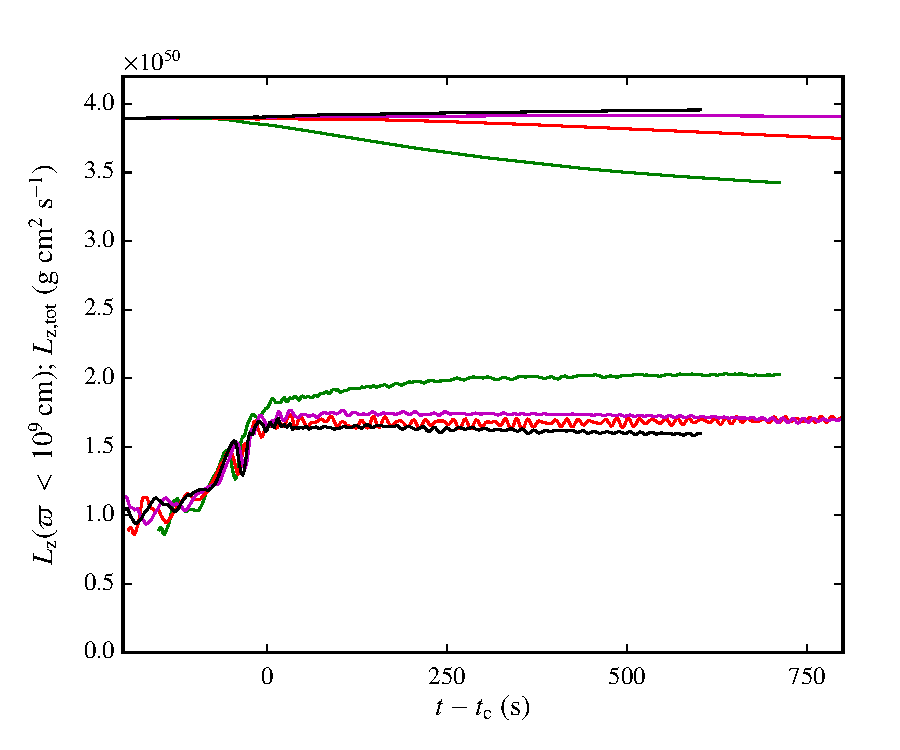
\includegraphics[angle=0,width=0.6\columnwidth]{chapter3_zhu+u/figures/lz_development2.pdf}
\caption{Evolution of total $z$-axis angular momentum \Lztot\ (top cluster of lines) and that within a cylinder of radius $\varpi = 10^9\,\mrm{cm}$, \Lzinner\ (bottom cluster) for the \arepo-RKLSF simulations.  All curves are shifted in time by \tcoal\ (rather than \tlm\ like in Fig. \ref{fig:c3_fix_angmo}), the time when average separation between donor and accretor material reaches a tenth of its initial value.  Colors indicate initial mass resolutions of $5\times10^{28}\,\mrm{g}$ (red lines), $1\times10^{28}\,\mrm{g}$ (green) $2\times10^{27}\,\mrm{g}$ (cyan) and $1\times10^{27}\,\mrm{g}$ (blue).}
\label{fig:c3_fix_angmo_nar}
\end{figure}

% green is for $5.1\times10^4$ cells, red for $2.5\times10^{5}$, magenta for $1.3\times10^{6}$ and black for $2.5\times10^6$.

In Fig. \ref{fig:c3_fix_angmo_nar}, we show the evolution of angular momentum for \arepo-RKLSF runs (from Sec. \ref{ssec:c3_restest}) at resolutions ranging from $5\times10^{28}\,\mrm{g}$ to $1\times10^{27}\,\mrm{g}$.  We immediately notice that \Lzinner\ no longer decreases with time, cementing the fact that the rapid spin-down seen in Fig. \ref{fig:c3_fix_angmo} was an artefact of spurious angular momentum loss.  Indeed, this makes it impossible to calculate \tlm\ -- we instead use ``\tcoal'' (discussed further in Sec. \ref{sec:c3_results}), the time when the average separation between donor and accretor material reaches a tenth of its value at the beginning of the simulation, to synchronize the start of post-merger evolution.  In all but the lowest-resolution run, \Lztot\ deviates by less than $\sim4$\% from its initial value, and at the highest resolution run of $1\times10^{27}\,\mrm{g}$, or $2.5\times10^6$ cells, it deviates by $\sim1.5$\% over $\sim840\,\mrm{s}$, an order of magnitude better than the $2\times10^7$ cell simulation without RKLSF.

The density and temperature profiles of the merger in the \arepo-RKLSF simulations also generally agree better with their \gasoline\ counterparts up until the end of coalescence, but the dense crescent and spiral wave that distinguish the \arepo\ merger remnant remain.

\section{Results}
\label{sec:c3_results}

% One orbit is 49.5 s

\begin{figure}
\centering
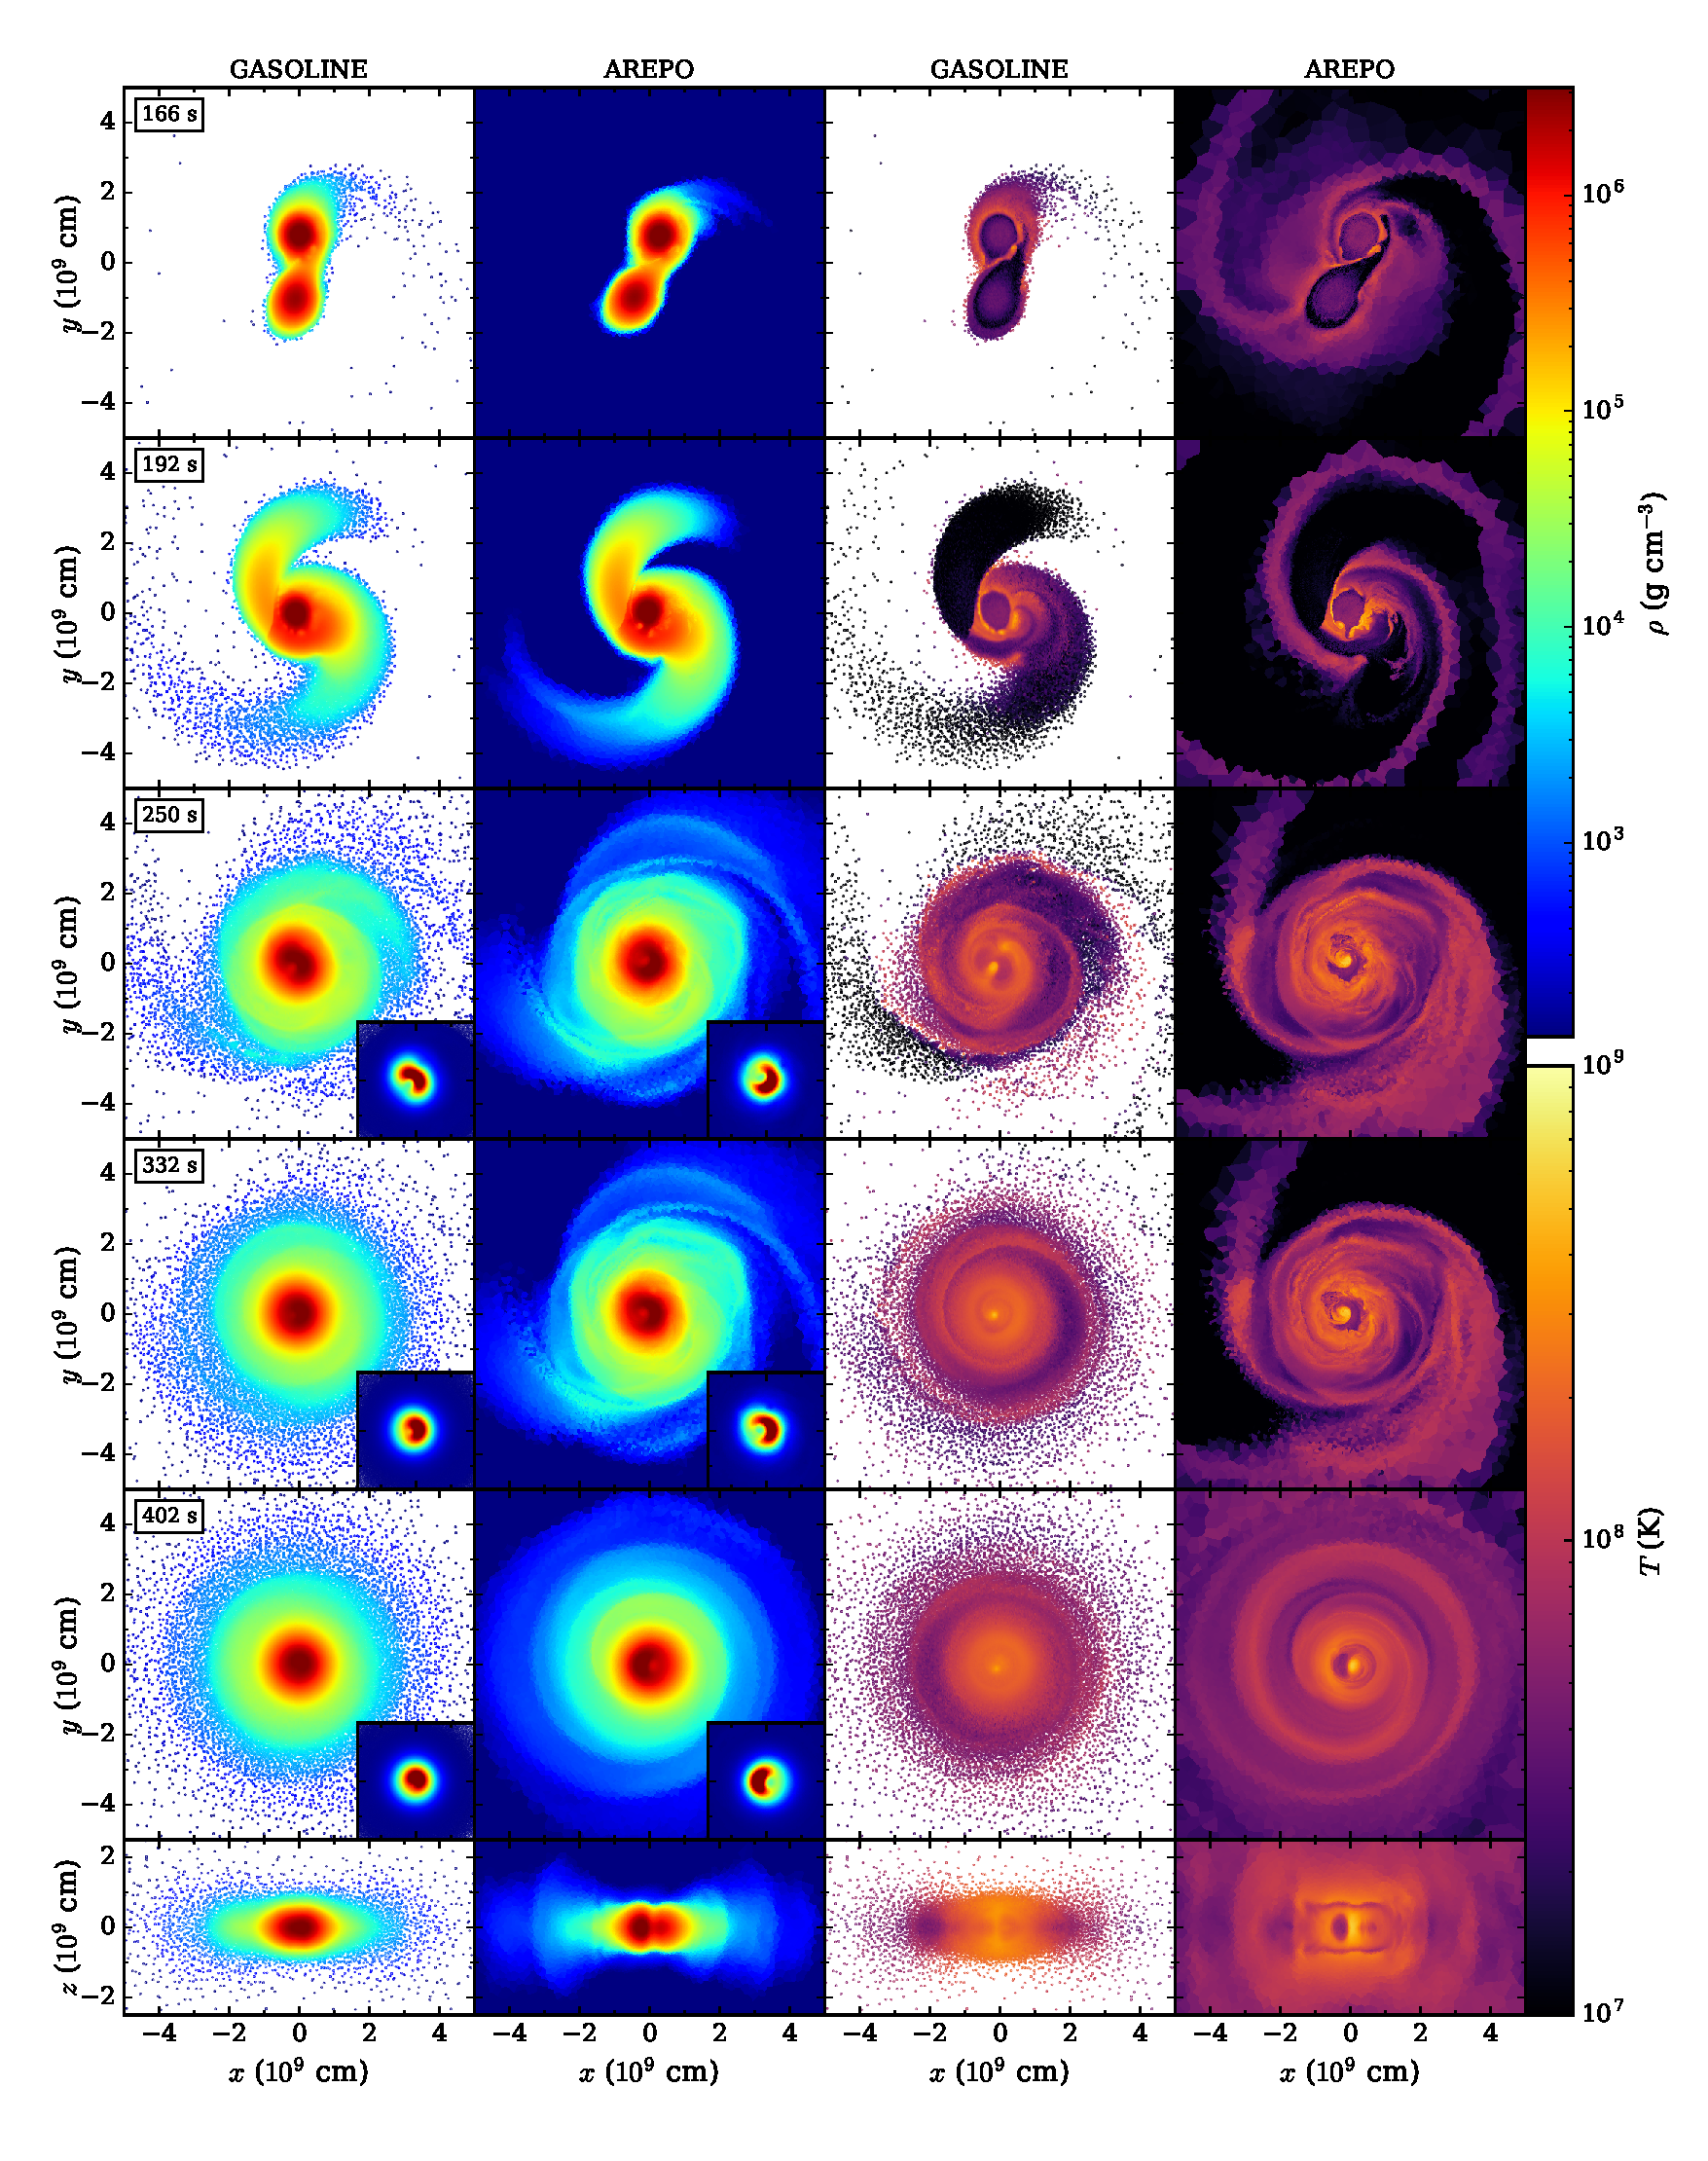
\includegraphics[angle=0,width=1.0\columnwidth]{chapter3_zhu+u/figures/snapshots.pdf}
\caption{Series of equatorial ($xy$) plane density (left two columns) and temperature (right two columns) intensity plots for five snapshots in time (rows; the time for each snapshot is indicated at the top left of the density plots) during the \gasoline\ and \arepo\ simulations.  $xz$-plane plots are also included for the final snapshot.}
\label{fig:c3_diagslice}
\end{figure}

We now compare in detail our new \arepo\ simulation with a \gasoline\ one.  Fig. \ref{fig:c3_diagslice} compares snapshots of the two at various times.

The initial evolution of the two systems, shown in row 1 of Fig. \ref{fig:c3_diagslice}, is qualitatively similar.  Our initial conditions are approximate, so both stars immediately are tidally stretched by the binary potential, overshooting their Roche lobes in the process and transferring mass to each other in spurts.  This eventually dies down for the $0.65\,\Msun$ accretor, and becomes steady mass transfer for the $0.625\,\Msun$ donor, just prior to it becoming fully disrupted.  In reality, the donor WD should overflow first and begin a period of quasi-stable mass transfer over potentially dozens of orbits, and so our simulations, both of which experience full donor disruption in just a few orbits, overestimate the rate of early mass transfer \citep{dan+11}.

% To check the mach number, I compared the velocity of the stream (in the frame of the accretor's center 2.5x10^8 cm/s) with the sound-speed of the outer layers of the accretor (1.3x10^8 cm/s).  Hot atmosphere temperatures from paper_propsatdisruption(frame="early")

The accretion streams in both codes are travelling at supersonic speeds ($\mathcal{M} \approx 2$) relative to the accretor when they impact, and the resulting shocks cause rapid thermalization.  By the time the donor is fully disrupted a hot atmosphere has formed around the accretor, with temperatures of $1.6 \times 10^8\,\mrm{K}$ in  \arepo\ and $1.9\times 10^8\,\mrm{K}$ in \gasoline\ -- both about a quarter of the virial temperature, $GM_am_P\mu/3R_ak_B \approx 7 \times 10^8\,\mrm{K}$ -- and densities of $1.8\times10^5\,\gcc$ and $2.3\times10^5\,\gcc$, respectively.  As can be seen in Fig. \ref{fig:c3_diagslice} row 1, \arepo's hot atmosphere is somewhat less extended and has more localized hotspots in temperature compared to the extended and uniform one in \gasoline.  This may be due to a combination of \arepo\ not oversmoothing the gradients within the atmosphere, and having superior spatial resolution for the same mass resolution.

% Note to self: M = 10 is cited by Guillochon et al. 2010 by comparing the Keplerian velocity to the local soundspeed.  I'm using the actual velocity compared to the soundspeed, which is apparently much lower.  At best, we can get M = 3.

As mass transfer continues to expand the donor and draw it closer to the accretor, eventually tidal forces between the two are strong enough to fully disrupt the donor, stretching it out into a thick stream of material that wraps around the accretor (see Fig. \ref{fig:c3_diagslice}, row 1).  In both simulations, this occurs after $\sim3.6$ orbital periods of the initial binary, or $\sim180\,\mrm{s}$, by which time the donor has transferred $\sim0.05\,\Msun$ to the accretor.  During coalescence, both the density and temperature profiles appear very similar between the codes, and the destruction of the donor takes place over the same amount of time -- about one orbital period ($49.5\,\mrm{s}$).

%Just read the KH blob temperatures off from the intensity plots at the disruption time of t = 180 s.  Lengths and widths were manually measured from the intensity plots with a temperature range of [3e8 to 6e8] and averaged between the three blobs for each simulation.  Peak temperatures visually read out of each blob and averaged for reported values.

Once the donor is fully disrupted, and coalescence begins, a portion of it forms an accretion stream that slides across the accretor at supersonic speeds, creating a string of Kelvin-Helmholtz vorticies.  In \arepo\ these vorticies are markedly more pronounced, being both larger by $\sim30$\% in radius, and having a slightly higher temperature of $\sim5\times10^8$ K compared to \gasoline's $\sim4\times10^8$ K.  The stream continues to inspiral toward the center of the accretor, severely deforming the accretor while carrying the string of Kelvin-Helmholtz vorticies toward the center of the system.  The two WDs have nearly equal masses, so material near the surface of the accretor is dredged up and mixes with the stream, and the shape of the accretor changes from a sphere into a crescent.  Meanwhile, the remainder of the donor material forms a thick sub-Keplerian disk around the accretor.  Coalescence is approximately complete when the average separation between material from the donor and accretor changes from its initial value of $2.2\times10^9\,\mrm{cm}$ to its equilibrium value of $\sim1\times10^8\,\mrm{cm}$.  We thus estimate the time when coalescence is complete, \tcoal, by determining the time when average donor-accretor separation reaches a tenth of its initial value.  We find $\tcoal = 228\,\mrm{s}$ for \gasoline, and $220\,\mrm{s}$ for \arepo\ (roughly Fig. \ref{fig:c3_diagslice}, row 3).

\begin{figure}
\centering
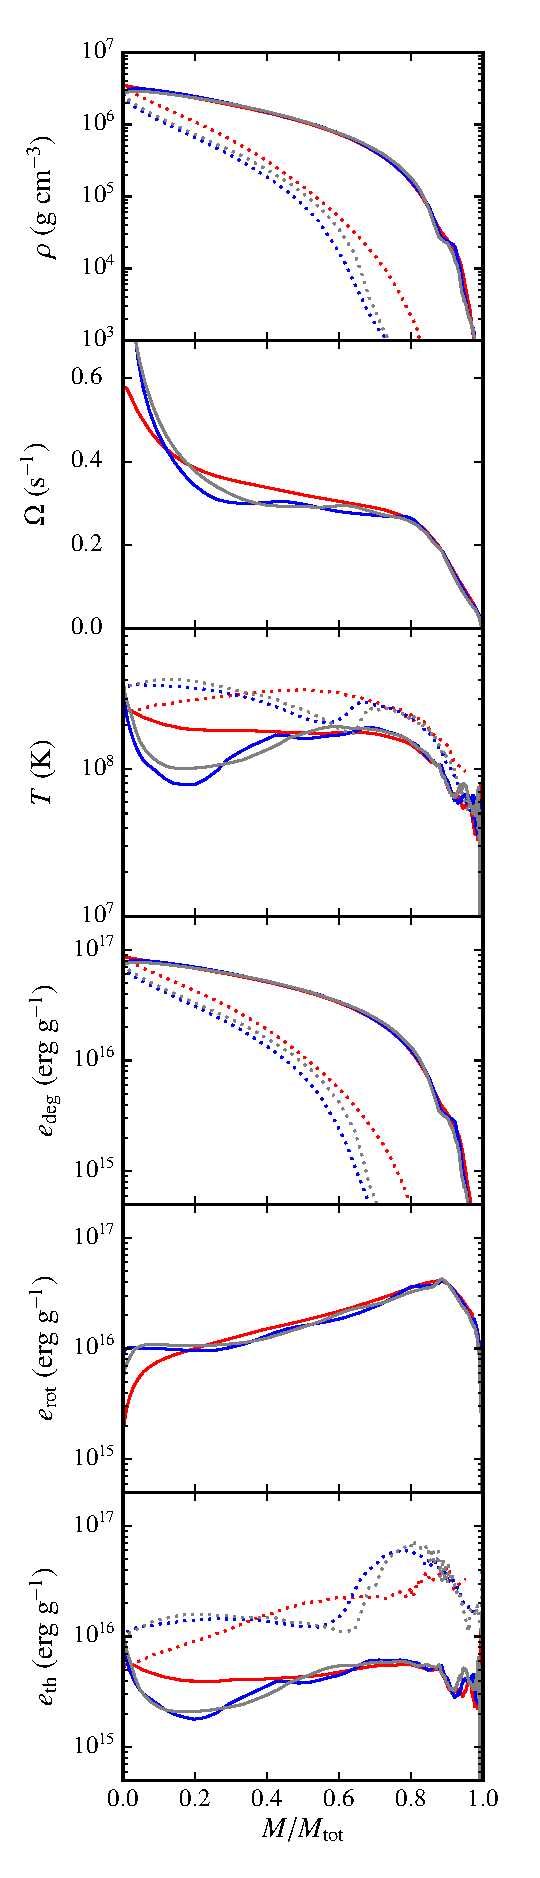
\includegraphics[angle=0,width=0.35\columnwidth]{chapter3_zhu+u/figures/curves.pdf}
\caption{Merger remnant profiles from the \gasoline\ (red), \arepo\ (blue) and \arepo\ MHD (gray; Ch. \ref{ch:ch4}) simulations $99\,\mrm{s}$ after coalescence (around row four of Fig. \ref{fig:c3_diagslice}).  The profiles are, from top to bottom, density $\rho$, angular rotation speed $\Omega$, temperature $T$, specific degeneracy energy  $e_{\rm deg}$, specific thermal energy $e_{\rm th}$, and specific rotational energy $e_{\rm rot}$, all as a function of the ratio of spherical enclosed to total mass $M/M_{\rm tot}$.  Solid lines represent profiles on the original binary's orbital plane, while dash-dotted lines represent profiles along the rotational axis.}
\label{fig:c3_curves}
\end{figure}

In Fig. \ref{fig:c3_curves}, we show profiles of density, temperature and energy for the merger remnants at $99\,\mrm{s}$ ($2$ orbital periods) after coalescence, roughly equivalent to row 4 of Fig. \ref{fig:c3_diagslice}.  Profiles both along the orbital plane of the original binary, or ``equatorial plane'' (solid lines) and rotational axis (dotted) are considered, and like in Ch. \ref{ch:ch2} we map (equatorial) $\varpi$ and (rotational) $z$ positions to the corresponding ratio of spherical enclosed mass to total mass $M/M_{\rm tot}$.  The equatorial profiles are axisymmetrically averaged, while the rotational axis ones are averaged from the profiles above and below the equatorial plane.  Overall, the two remnants have very similar structures: both feature a degeneracy-supported core surrounded by a rotationally supported thick disk along the equatorial plane and by a hot, thermally supported atmosphere along the axis of rotation.  Following Sec. \ref{sssec:c2_masstrends}, we find the disk mass $\Mdisk = 0.24\,\Msun$ and the core-envelope mass $\Mrem = 1.05\,\Msun$ in both simulations, though we note that the core-envelope also has substantial rotational support throughout.\footnote{The mass of material whose specific degeneracy energy is $>50$\% of their total specific energy is $\sim0.8\,\Msun$ in both simulations, as it is in Ch. \ref{ch:ch4}.}  Both remnants' total internal energies ($1.5\times10^{50}\,\mrm{erg}$) are also identically divided into $\sim30$\% rotational, $\sim10$\% thermal and $\sim60$\% degeneracy energy.  One minor difference between the two codes is the total amount of material unbound by the merger -- $1.4\times10^{-3}$ \Msun\ in \gasoline, and $5.0\times10^{-4}$ \Msun\ in \arepo -- though this value is much smaller and harder to constrain than the bulk values above.

% The unbound values take total energy into account, not just kinetic!

% Values below read off Fig fig:curves using ipython.  If you just look at the 1000 densest particles/cells, the density is 4e6 gcc (from snapshots 99 sec after coalescence).

The simulations' profiles in Fig. \ref{fig:c3_curves} are likewise very similar in shape to one another: both, for example, have a peak density of $\sim3\times10^6\,\gcc$ and a large fraction of their mass rotating nearly rigidly at $\sim0.3\,\psec$.  We also show the \arepo\ MHD simulation from Ch. \ref{ch:ch4} in grey, and find it is similar as well, indicating that including magnetic dynamo effects lead only to minor changes in the \textit{hydrodynamics} of the merger.  The greatest discrepancy is in the temperature at small $M/M_{\rm tot}$: it is a factor of $\sim2$ smaller in the \arepo\ simulation than in the \gasoline\ one.

% Used max values from paper_cicomp_hotmix(res="high"), double checked by examining images.  Void size obtained from examining images.  Gasoline final temperature obtained by averaging temperature of material >1e5 gcc in the 100000.ascii snapshot; structure obtained by examining xy AND xz temperature structures for snapshots after 100000.ascii.

% Pattern speed determined by watching movies and timing the spiral wave and crescent; base of spiral determined using paper_spiralwave()

That discrepancy, however, reflects a growing difference visible in rows 4 - 6 of Fig. \ref{fig:c3_diagslice}.  Just after coalescence, the center of the merger remnant in both simulations is clearly divided between a dense and cold crescent-shaped region, formed from the perturbed accretor WD, and a low-density void that is an order of magnitude hotter, formed by material roughly evenly mixed between donor and accretor (this void appears as a column in the $xz$ plots of Fig. \ref{fig:c3_diagslice}).  $99\,\mrm{s}$ after coalescense, the hot void has a temperature of $\sim6\times10^8\,\mrm{K}$ in both codes, but the \arepo\ void is $\sim80$\% larger in radius and slightly less dense at $\sim1.5\times10^6\,\gcc$ versus \gasoline's $\sim2\times10^6\,\gcc$.  The cold crescent, meanwhile, has a density of $\sim4\times10^6\,\gcc$ in both codes, but has a temperature of $\sim2\times10^8\,\mrm{K}$ in \gasoline\ versus $\sim5\times10^7\,\mrm{K}$ in \arepo.  Over the next several hundred seconds, the \gasoline\ remnant's crescent becomes axisymmetric, eliminating the hot void in the process; material from the void moves off of the equatorial plane to form two $\sim3.5\times10^8\,\mrm{K}$ hotspots along the rotational axis (row 6 of Fig. \ref{fig:c3_diagslice}).  By $t\approx500\,\mrm{s}$, the \gasoline\ remnant structure -- an oblate spheroidal core with a roughly uniform temperature of $\sim 2 \times 10^8\,\mrm{K}$ (outside of the hotspots) surrounded by a stubby disk -- has stopped changing on a hydrodynamic timescale (roughly equal to one binary orbital period).  \arepo, on the other hand, maintains the distinction between the crescent and void, and consequently remains non-axisymmetric until the end of the simulation at $1000\,\mrm{s}$.  The system's center of rotation and mass are at the midpoint along the boundary between the crescent and void, and the dense crescent revolves around this point (rather than spinning about it).  This generates a lopsided gravitational potential that perturbs the surrounding disk, launching an $m = 1$ one-armed spiral wave into the surrounding medium.  The pattern speed is $\Omega_p \approx 0.4\,\mrm{s}^{-1}$ (as is the angular speed of the crescent), and the base of the spiral wave is at $\varpi \approx 1.5\times10^9\,\mrm{cm}$, where $\Omega \approx 0.2\,\mrm{s}^{-1}$ -- in 2:1 resonance with the crescent.

\begin{figure}
\centering
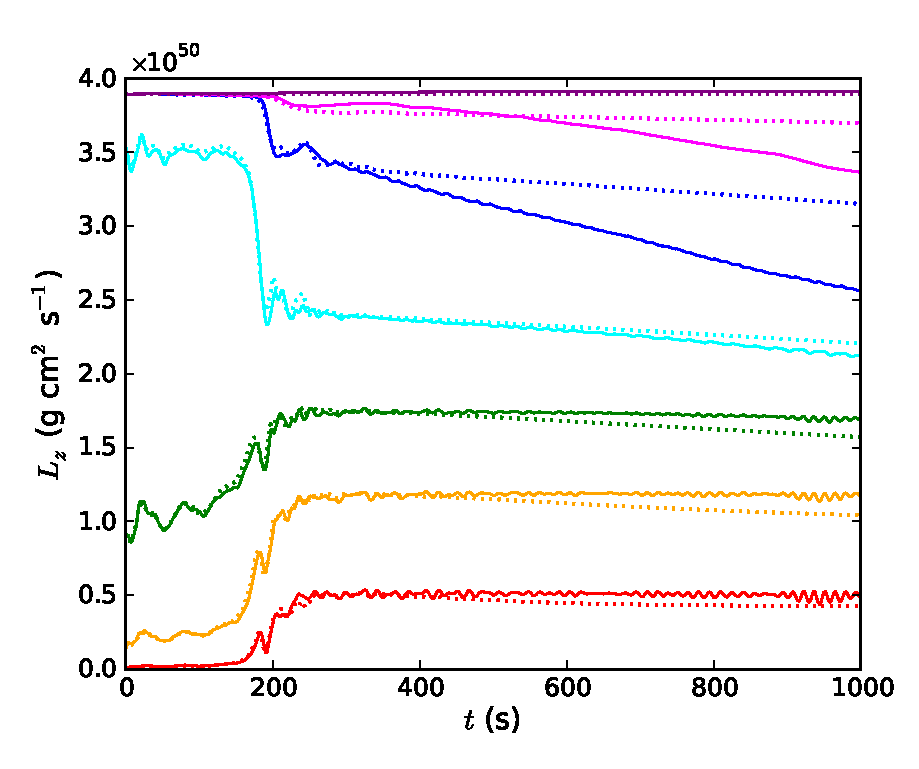
\includegraphics[angle=0,width=0.6\columnwidth]{chapter3_zhu+u/figures/Lz.pdf}
\caption{Time evolution of $z$-axis angular momentum \Lz\ for \arepo\ (solid lines) and \gasoline\ (dashed) simulations.  The purple line represents total \Lz, while the others represent angular momentum within concentric cylinders aligned along the rotation axis and with radii $\varpi = 5\times10^8$ (red), $7.5\times10^8$ (yellow), $1\times10^9$ (green), $1.5\times10^9$ (cyan), $3\times10^9$ (blue) and $6\times10^9\,\mrm{cm}$ (magenta).}
\label{fig:c3_angmo}
\end{figure}

Since spiral waves can transport angular momentum, we show in Fig. \ref{fig:c3_angmo} the evolution of $z$-axis angular momentum \Lz\ within concentric cylinders centered on the rotational axis for the two simulations.  We see that all cylinders slowly lose angular momentum after colaescence in the \gasoline\ simulation, consistent with the effect of artificial viscosity.  In \arepo, $\Lz(\varpi < 3\times10^9\,\mrm{cm})$ decreases at a rate of $d\Lz/dt = 1.2\times10^{47}\,\mrm{g}\,\mrm{cm}^2\,\mrm{s}^{-2}$ (compared to $3.3\times10^{46}\,\mrm{g}\,\mrm{cm}^2\,\mrm{s}^{-2}$ in \gasoline), reflecting the wave's angular momentum transport.  Applying Eqn. \ref{eq:c3_angmobalance} to the cylinder, we estimate around $\sim85$\% of this decrease can be accounted for by advection, suggesting the spiral wave transports angular momentum through Reynolds stresses (rather than gravitational torque; \citealt{kratl16}).  The angular momentum within \innercyl\ decreases by $\sim5$\% by the end of the simulation at $t = 1000\,\mrm{s}$, but the loss of angular momentum in the disk also results in the enclosed mass within \innercyl\ increasing by $0.02\,\Msun$ over the same timeframe.  In fact, the remnant disk has transported about half of its angular momentum to much larger distances by this time; the corresponding timescale is roughly equal to that for an $\alpha$-viscosity disk with $\alpha \sim 10^{-1}$.  For comparison, \cite{ji+13} simulate the magnetically-mediated viscous evolution of a $0.6-0.6\,\Msun$ merger remnant, and find angular momentum transport at a rate equivalent to an $\alpha = 10^{-2}$ disk, an order of magnitude smaller.  At $t = 1000\,\mrm{s}$, \arepo's void has shrunk by about a quarter of its initial radius, but the remnant core remains non-axisymmetric and the spiral wave persists, and so angular momentum transport should continue on a hydrodynamic timescale beyond the end of the simulation.

Preliminary attempts to carry the simulation even further in time in \arepo, however, have been stymied by the spurious formation of a $<10^7\,\mrm{K}$ ring of material at the interface between donor and accretor at $\sim1000\,\mrm{s}$.  The appearance of this numerical artefact, which appears at an earlier time at the lower-resolution simulations in Sec. \ref{ssec:c3_restest}, is troubling, and suggests that \arepo\ must be further refined before the full hydrodynamic spin-down of the remnant can be simulated.  We therefore caution that the values stated above may not be accurate, particularly close to the end of the simulation, though (since our highest resolution run in Sec. \ref{ssec:c3_restest} does not develop this issue) our qualitative results are more robust.

%Under both codes, the remnant core is a cresent-shaped object off of the centre of rotation, flanked on one side by a low-density hot void, and therefore features a prominent $m = 1$ non-axisymmetric mode that we expect to either gravitationally torque or hydrodynamically stir the surrounding medium.  Disturbances generated by the core will naturally be stretched out into a trailing spiral pattern due to the differential rotation of the sub-Keplerian disk.

%\arepo, on the other hand, maintains the integrity of the cresent and void for hundreds of seconds.  In the high-resolution simulation, by $t = 200$ s, a single spiral with a $\delta \rho/\left\langle\rho\right\rangle$ of $\sim1$ and Mach number $\mathcal{M} \approx 2$ is generated, either through ram pressure, tides, or by a combination of the two, near the transition between the remnant core and disk.  Once generated, they hydrodynamically transport angular momentum outward before disappearing past $10^{10}$ cm, accounting for the strong \Lzinner\ loss seen in Fig. \ref{fig:angmo}.  Some dissipation occurs before the shock reaches $10^{10}$ cm, though, as we also find an outward mass flux throughout the entire disk, and a gain in angular momentum for material past $\sim3\times10^9$ cm.  These shocks also do not propagate only along the mid-disk: they trace out expanding semicircular arcs in the $r_\mrm{xy}-z$ plane, spreading material beyond the plane of the disk in a fan shape.

%\arepo, on the other hand, maintains the coherency of its void over hundreds of seconds as the torus of dense material deforms into a crescent and hydrodynamically launches a single spiral wave into the surrounding medium.  Over time, this spiral wave transports angular momentum away from the core, allowing the crescent to sink toward the remnant center of mass.  This is radically different than what we see in \gasoline, and has not been reported by other SPH simulation works, which suggests that there is a phase of hydrodynamic evolution following coalescence that is not properly captured by traditional SPH.  Unfortunately, issues with angular momentum conservation in \arepo\ prevent us from reliably following this post-merger hydrodynamic evolution further than a few hundred seconds, and we cannot definitely say if the remnant core is able to lose much of its angular momentum via spiral waves.  This issue is further discussed in Sec. \ref{ssec:pmeloss}.

%We have attempted to extend this simulation by several thousand seconds to probe the long-term stability of the remnant's structure, but find instead the spontaneous development of a dense $<10^7\,\mrm{K}$ layer (much colder than any material surrounding it) at the boundary between the remnant core and disk.  

\section{Discussion}
\label{sec:c3_discussion}

To determine the robustness of our results, and provide clues to the sources of the differences between \arepo\ and \gasoline\ simulations, we ran a number of tests varying code parameters.

\subsection{Resolution Test}
\label{ssec:c3_restest}

%low and high-resolution \arepo\ simulations experience initial mass transfer at about twice the rate of their \gasoline\ counterparts -- the accretion stream is correspondingly denser -- and experience donor disruption at approximately three orbits of the binary, rather than {\gasoline}'s four.  Two factors can contribute to this difference.  First (and based on Sec. \ref{ssec:restest}, perhaps most important), because steep density gradients near the surface of the WDs are treated differently in the two codes, and \arepo\ requires a background grid, stars relaxed in {\gasoline} tend to expand a little when transferred to {\arepo}.  Second, mass transfer in SPH can only occur by passing particles between the WDs, imposing a mass resolution limit, while in \arepo\ no such limitation exists.  This second issue exists even at the highest resolution SPH simulations performed to date, and detailed studies of the accretion stream are best done using a grid code to complement or supplement the SPH simulation \citep{guil+10, ross14}.

As noted in Sec. \ref{ssec:c3_initcond}, an \arepo\ simulation with identical mass resolution to a \gasoline\ one will have roughly a factor of {\charles $3$} higher spatial resolution because of the 100 neighboring particles used by the kernel.  It is possible that the differences we observe between our simulations are not due to fundamental differences between the codes, but because our \gasoline\ simulation insufficiently resolves the merger.  To address this, we perform a series of \gasoline\ and \arepo\ simulations with a mass resolutions of $5\times10^{28}\,\mrm{g}$ (equivalent to $5.1\times10^4$ particles/cells and comparable to resolutions used in parameter-space sweeps \citealt{dan+12,dan+14}), $1\times10^{28}\,\mrm{g}$ ($2.6\times10^{5}$) and $1\times10^{27}\,\mrm{g}$ ($2.6\times10^{6}$).  This factor of $50$ range in mass resolution ($\sim4$ in spatial resolution) allows us to both determine the degree to which mergers in each code change with resolution, and to compare \arepo\ runs to \gasoline\ ones at finer mass resolution.

At all four resolutions, the \gasoline\ simulations exhibit very similar behavior prior to coalescence.  The donor fully disrupts in at $\sim3.5$ orbits of the initial binary for the two higher resolution runs, while the two lower-resolution ones disrupt slightly earlier at $\sim3.2$ orbits ($\sim155-160\,\mrm{s}$).  Coalescence for the highest resolution run occurs at $\tcoal = 230\,\mrm{s}$, within $2$ seconds of the standard resolution one, while it occurs $15 - 30$ seconds earlier for the two lower resolution runs (we note the way we determine coalescence is somewhat sensitive to changes in the detailed configuration of the remnant).  Just after coalescence, all reproduce the crescent-and-void configuration, with the void being least prominent in the lowest-resolution run.  

\arepo\ also reproduces the same qualitative evolution up to coalescence at all resolutions, but donor disruption occurs within only $\sim2$ orbits at its lowest resolution, and in $\sim3$ at its second lowest.  The time of coalescence is likewise much sooner in the lowest resolution simulation, with $\tcoal = 150\,\mrm{s}$.  The highest resolution run, however, is very similar to the standard resolution one, with donor disruption occuring at $\sim180\,\mrm{s}$ and $\tcoal$ occuring at $234\,\mrm{s}$, close to the standard run's values.  These differences are in part due to our initial conditions setup, where \gasoline\ SPH particles are directly mapped to \arepo\ cells.  WDs that are hydrostatic in \gasoline\ are not precisely so in \arepo, particularly in the poorly resolved atmosphere, and we see the WDs spuriously expanding in the first few seconds.  This effect leads to larger mass-transfer rates early in the merger, and is magnified with decreasing resolution.  Just after coalescence, all reproduce the crescent-and-void configuration except in the lowest-resolution run.

% Personal note on initial conditions: as described by Agertz et al. 2007 and Hess & Springel 2010, surface tension applies at the interface between two fluids of differing densities but the same pressure.  As particles from the less dense fluid approach the interface, they begin sampling only the density of the denser fluid (since they comprise the majority of nearby particles).  This overestimates incoming particles' densities, leading to an additional repulsive force that inhibits mixing.  I understand the qualitative picture (the SPH equation of motion uses only the density of the local particle, not its mass, so an increase in density is equivalent to an increase in mass, and this becomes a bigger and bigger problem as the particle approaches the interface, thereby reducing accelerations; these accelerations "go back to normal" as the particle moves away).  I'm unable to replicate it in equations though.  I suspect that for hydrostatic equilibrium, what's happening is that particles at the surface of the star will both have spuriously high densities and forces coming from only one side.  The latter is simply a poor estimate, but the former is a systematic offset that will shrink the size of the star and, when we map our SPH initial conditions into Arepo, create systematically high densities in the outermost layers of the star.  This means we're making a star that's missing its outer layers (because SPH doesn't have the mass resolution) and piling that material slightly deeper down in the star.  In Arepo, this would act like a spring, leading to more violent oscillations.  I'm not certain why the final state of the relaxed star in Arepo has lower central density - perhaps because the atmosphere is heated more from the oscillations, the center sees less weight?

% The lowest resolution merger in Arepo also seems to heat a bit more prior to the merger, which might be due to a combination of the hydrostatic equilibrium issue and 

\begin{figure}
\centering
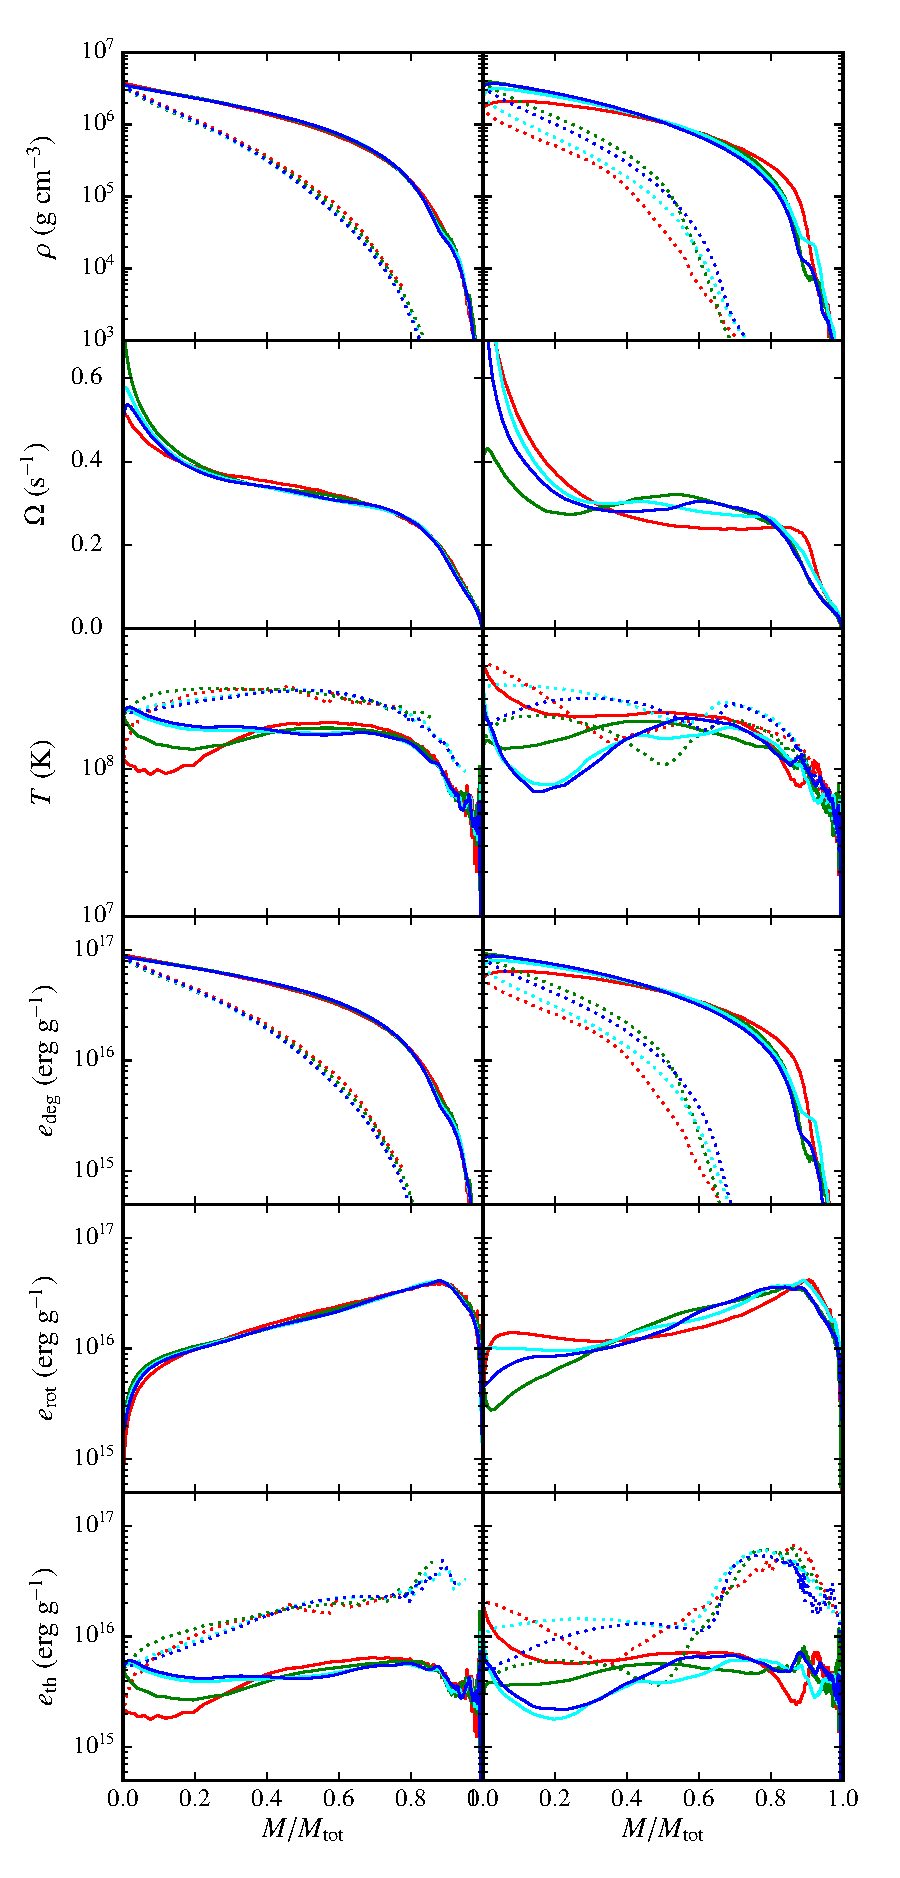
\includegraphics[angle=0,width=0.6\columnwidth]{chapter3_zhu+u/figures/curves_res.pdf}
\caption{Merger remnant profiles, as in Fig. \ref{fig:c3_curves}, for \gasoline\ (left column) and \arepo\ (right) simulations of various (initial, for \arepo) mass resolutions.  The resolutions are $5\times10^{28}\,\mrm{g}$ (equivalent to $5.1\times10^4$ particles/cells; red lines), $1\times10^{28}\,\mrm{g}$ ($2.6\times10^{5}$; green) $2\times10^{27}\,\mrm{g}$ ($1.3\times10^{6}$; cyan) and $1\times10^{27}\,\mrm{g}$ ($2.6\times10^{6}$; blue).}
\label{fig:c3_res_curves}
\end{figure}

In Fig. \ref{fig:c3_res_curves}, we plot the equatorial and rotational axis profiles of all simulations $99\,\mrm{s}$ after \tcoal.  The \gasoline\ remnants (left column) are all remarkably similar to one another, with the sole exception of the temperature structure at the lowest resolution.  The disk and core-envelope masses as well as the partitioning of internal energy are all within $1$\% of their values at standard resolution reported in Sec. \ref{sec:c3_results}.  The central density also deviates by $\lesssim3$\% from $3.6\times10^{6}\,\gcc$ in all remnants.  The \arepo\ remnants (right column) are less uniform: masses and energies vary by $\sim10$\% from those in Sec. \ref{sec:c3_results}, and the maximum density ranges from $3-4\times10^6\,\gcc$ for all resolutions except the lowest one, where it is $\sim2\times10^6\,\gcc$.  The variations between \arepo\ curves in Fig. \ref{fig:c3_res_curves} reflect variations their crescent and void.  While at the highest two resolutions the crescent is clearly colder, with a temperature of $\sim6\times10^7\,\mrm{K}$, at a resolution of $1\times10^{28}\,\mrm{g}$ the crescent's temperature is $3\times10^8\,\mrm{K}$, and at the lowest resolution the remnant's core never forms a crescent at all, instead appearing as a dumbbell-shaped object that transforms into a spherically symmetric one within $500\,\mrm{s}$ of coalescence.  During this time, global angular momentum decreases by $\sim10$\% (Fig. \ref{fig:c3_fix_angmo_nar}), and a $<10^7\,\mrm{K}$ ring of material spurious forms at the interface between donor and accretor, both indicating that the \arepo\ is too poorly resolved to simulate the merger.  At all other resolutions, however, the crescent and void survive until the end of the simulation at $1000\,\mrm{s}$.

The crescent-void configuration also appears, but then fades away over several hundred seconds, in all \gasoline\ simulations.  To check if the longevity of the configuration is resolution-dependent, we turn to \citeal{zhu+13}'s measurement of non-axisymmetry using $|f_i|/|f_0|$, the ratio of largest non-zero to zeroth Fourier coefficient of particles or cells binned in azimuth.  For all simulations, the largest non-zero Fourier coefficient is the first, and the time when the hot void disappears roughly matches the time when $|f_1|/|f_0| = 0.01$, which we call $t_f$.  We find, from lowest to highest resolution, $t_f = 425\,\mrm{s}$, $483\,\mrm{s}$, $515\,\mrm{s}$ and $513\,\mrm{s}$, which suggests $t_f$ is resolution dependent, but convergence at $t_f \approx 500\,\mrm{s}$.   All \arepo\ simulations maintain $|f_1|/|f_0| \gtrsim 0.1$ for $\gtrsim 1000\,\mrm{s}$, except for the lowest-resolution run, which drops to $|f_1|/|f_0| \approx 0.02$ by the end of the simulation.

%-- roughly corroborated by visual inspection of the remnant's non-axisymmetry --

We thus conclude that the largest difference between the \gasoline\ and \arepo\ simulations -- the survival of the crescent-void configuration long after the merger -- is the case for all resolutions.  The void persists for hundreds of seconds in all but the lowest-resolution \arepo\ simulation, while even in the highest-resolution \gasoline\ one it smears away, disappearing within $\sim 250$ s after coalescence.  This is evidence that spatial resolution alone is insufficient to explain the diverging behavior of the codes.  We also find that \gasoline's results change little between all resolutions, while \arepo's results only appear to agree at higher resolutions.  This bodes well for merger parameter-space studies using low-resolution SPH simulations (eg. \citeal{zhu+13}, \citealt{dan+14}; the latter finds similar results in their resolution study unless nuclear burning becomes important during the merger), but an equivalent study in \arepo\ would require a mass resolution finer than $\sim1\times10^{28}\,\mrm{g}$ (and ideally closer to our standard resolution of $2\times10^{27}\,\mrm{g}$) to guarantee qualitative accuracy with higher-resolution runs.

\subsection{Varying Viscosity in \gasoline}
\label{ssec:c3_vary_visc}

Artificial viscosity, which is essential in SPH for proper shock capture, has been a major issue for white dwarf merger simulations for decades (eg. \citealt{guerig04, loreig09}) because it spuriously shears differential rotation into rigid rotation, dumping excess energy into heat.  This viscosity cannot simply be mitigated by resolution, and we cannot run our mergers with zero artifical viscosity without neglecting shock heating and introducing unphysical particle behavior (Sec. \ref{ssec:c3_sph}).  We can, however, increase and reduce its strength to see what effect it has on our simulation results, as in \citeal{zhu+13} {\charles Sec. XXX}.

We ran \gasoline\ simulations of our merger with a mass resolution of $1\times10^{28}\,\mrm{g}$ and artificial viscosity with fixed coefficients of either $\alpha\,=0.05$, $\beta\,=0.1$, or $\alpha\,=1$, $\beta\,=2$ (the Balsara switch is still active), comparing them to the variable-viscosity run at the same resolution in Sec. \ref{ssec:c3_restest}.  These simulations both experience donor disruption after $\sim3.2$ binary orbits, similar to the variable-viscosity one, and coalescence occurs at $205\,\mrm{s}$ and $219\,\mrm{s}$ for the low and high-viscosity runs, respectively.  This similarity is to be expected, since mass transfer and donor disruption are governed by tidal forces, which are unchanged between the simulations.  During coalescence, the evolution of the variable and high-viscosity runs is similar.  In the low-viscosity run, however, the donor's accretion stream produces a contiguous hot ring around the accretor during coalescence, rather than the string of vortices seen in row 2 of Fig. \ref{fig:c3_diagslice}, and perturbes the accretor far less.  As a result, no distinct void ever forms, though the remnant core is distorted into a bean shape.  Within $\sim25\,\mrm{s}$ of coalescence, the void in the high-viscosity simulation is already fast-disappearing, having a radius less than half that of the variable-viscosity run.  $t_f = 358\,\mrm{s}$ and $486\,\mrm{s}$ for the high and low-viscosity runs, respectively, compared to $483\,\mrm{s}$ for the variable one.  The similarity of the latter two values is likely because the variable-viscosity run tends toward the same $\alpha$ and $\beta$ values as the low-viscosity one in the absence of shocks (though it may also partly be coincidence, since the low-viscosity remnant does not have a hot void to begin with).  At $\sim500\,\mrm{s}$, the remnant has become axisymmetric in all three codes, but in the high-viscosity run the interior $\sim0.8\,\Msun$ of the remnant is also rigidly rotating with $\Omega = 0.33\,\mrm{s}^{-1}$, and features a nearly uniform temperature of $2 - 2.5\times10^8\,\mrm{K}$. 

As expected, then, the high-viscosity simulation rapidly spins down to axisymmetry while eliminating differential rotation, showing that excess artificial viscosity contributes to the disappearance of the crescent-void configuration.  The low-viscosity simulation, on the other hand, primarily shows the importance of increasing $\alpha$ and $\beta$ during coalescence in order to properly capture shocks and shearing interactions between donor and accretor.

% Void sizes use the DENSITY intensity maps, not temperature.

\subsection{Differences in the Merger Process}
\label{ssec:c3_differences_merger_process}

What explains the differences between simulations in \gasoline\ and \arepo, and, critically, which is more physically accurate?  This question boils down to whether or not the crescent-and-void configuration should be long-lived, as seen in \arepo, or should disappear over several hundred seconds as the remnant becomes axisymmetric, as seen in \gasoline.

Instabilities generating persistent $m = 1$ spiral waves that carry away angular momentum are a common feature of astrophysical disks, and have been studied, for example, in the contexts of star formation \citep{adamrs89, shu+90, lin15, kratl16} and supermassive black hole accretion \citep{hopkq10}.  We are, however, aware of only one other WD merger simulation with these features: \citep{kash+15} map the merger of a (highly super-\Mch) $1.0-1.1\,\Msun$ CO WD merger immediately after coalescence into \flash, and find that the merger remnant core, though not crescent-shaped, drifts off of the center of rotation and drives an $m = 1$ spiral perturbation in the disk around it for $\sim100\,\mrm{s}$.  They argue this is a variant of the ``ARS'' instability \citep{adamrs89, shu+90}, where, for a star surrounded by a Keplerian disk that is Toomre-stable ($Q \lesssim 3$), non-axisymmetric displace the central body off the system's center of mass and generate a gravitational instability in the disk that manifests as an $m = 1$ spiral wave.  Meanwhile, recent Eulerian simulations of binary neutron star (NS) mergers \citep{pasc15, radibo16} do see the formation of a crescent-and-void configuration with corresponding $m = 1$ spiral instabilities.  \citep{pasc15} attributes the formation of their spiral wave to a dynamic instability \citep{cent+11, saibs03} found to occur in axisymmetric equilibrium polytropes with toroidal density structures that have $T/|W| \gtrsim 0.14$, a relatively soft $n \lesssim 2$ polytropic EOS and high differential rotation \citep{saibs03}.  A similar phenomenon was observed by \cite{ott+05} to spontaneously develop in their post-bounce core-collapse supernova core of $T/|W| \approx 0.08$.  \cite{watt05} and \cite{wattaj05} note this instability may be a corotational shear instability, related to the \cite{papap84} instability for thick accretion torii.

% The cent+11 doesn't last forever - once the spiral destroys the crescent, it dies away (Saijo+03)

The conditions within our remnant are somewhat different than either of these instabilities: unlike the ARS setup, our inner disk is thick (scale height and disk radius are within an order of magnitude of each other) and has a Toomre paraometer of $Q \approx c_s\Omega/\pi G \Sigma \gtrsim 5$ for $\varpi \gtrsim 1\times10^9\,\mrm{cm}$ (where $\Sigma$ is the disk surface density; this is a factor of a few higher than those in \citealt{kash+15}).  The remnant core is already heavily perturbed at the start of post-merger evolution, and the spiral mode visible once the trasient features from the merger itself dissipate, making it difficult to identify a period of growth for the instability.  The behavior of our \arepo\ merger remnant may represent some combination of these instabilities, or possibly a novel, but related, phenomenon.  Further analysis is needed, but for now the existence of other $m = 1$ instabilities that drive angular momentum transport lends support to the physical validity of our results.

Note that in \citep{kash+15}, the spiral wave drives an inflow of hot material into the dense remnant core, and at $109\,\mrm{s}$ the base of the inflow detonates, driving a shockwave through the remnant that destroys it and synthesizes $\sim0.65\,\Msun$ of \Ni.  The spiral wave accretion in our sub-\Mch\ remnant reaches $\sim3\times10^8\,\mrm{K}$, well below the $\sim6\times10^8\,\mrm{K}$ neede for carbon ignition.

At the time of this writing, we have not yet conclusively pinpointed which features in \gasoline\ cause its simulations to differ from \arepo's.  Nevertheless, we discuss below a few hints that may point the way forward.  It should first be said that simulations of gravitational instability in protoplanetary disks have long been successfully simulated in SPH \citep{ricela05, merub10, rogew12}, and for the $\sim200\,\mrm{s}$ that the remnant core is visibly non-axisymmetric, an $m = 1$ spiral mode is also visible.  This leads us to suspect that the difference resides in how the crescent is evolved in SPH (though we leave open the possibility that the smearing out of the wavefront due to poor resolution in the disk is also a contributing factor).  The high-viscosity run in Sec. \ref{ssec:c3_vary_visc} suggests artificial viscosity may play a role in prematurely smearing out the crescent even when $\alpha$ and $\beta$ are being dynamically controlled.  Another possible culprit is the surface tension that results from poor discontinuity treatment in traditional SPH, which \cite{hesss10} shows can lead to an overdense ellipse at pressure equilibrium with its underdense surroundings spuriously deforming into a sphere.  While the boundary between the crescent and void is not as sharp a discontinuity, the temperature and density do change by a factor of $3$ over a single smoothing length, and so may be influenced by this effect.  We can test if this is the case by performing the same SPH merger using \textsc{Gasoline2}, which has improved entropy mixing and pressure-averaging across discontinuities.

%\cite{dval+06} performed an extensive battery of tests on 17 independent codes, 15 Eulerian and 2 SPH, simulating in two dimensions a planet on a circular orbit interacting with a protoplanetary disk.  The planet is expected to tidally excite a spiral wave from each of its two Lindblad resonances and open a density gap in the disk.  The Eulerian codes all reproduced these broad features as well as a number of non-linear ones such as vorticies at the, and their azimuthal and radial density profiles broadly agreed in shape - in many cases they numerically agree to within a few percent \textbf{check with pavel?}.  The SPH codes, on the other hand, produce gaps with poorly resolved boundaries (or in the case of shallow gaps, a poorly resolved gap in its entirety) and highly diminished spiral waves.  SPH density density profile had both different shapes and substantial systematic offsets.  Consequently, the tidal torques between the sprial waves and the planet measured by the Eulerian codes was far stronger than the torques measured by the SPH codes.  \cite{dval+06} speculated these differences were due to the diffusive nature of SPH, as well as code features like the Balsara switch designed to reduce viscosity in shear flows also leading to poor shock capture in those same regions.

%Artificial viscosity has long been cited as hindering the formation of spiral shocks under conditions theoretically favourable to their production (ex. \citealt{yukabm97, lanzb97, lanz03}).  In particular, sprial waves more readily develop in 2D disk simulations than in 3D due to the reduced effect of artificial viscosity in 2D \citep{lanz03}.  \cite{lanz10} attempts a more physically realistic implementations of artificial viscosity, and find stronger spiral waves develop in accretion disks as a result.

%%\lanza 10 a attempt to mitigate artificial viscosity by, and \lanza 10 replaced artificial viscosity in the SPH momentum and energy equations with an equation of state that captures the increase in pressure due to physical dissipation.  Tests using these modifications show much stronger accretion disk spiral waves than equivalent standard SPH simulations.

%%COMMENT: The papers cited above are annoyingly hard to read.  In lanza 10 b, the general implementation of the EOS results in an accretion ring rather than a disk.  Lanzafame cites this as being because physical dissipation is necessary for maintaining an accretion disk.

%-In early stages, artificial viscosity in Gasoline greatly increase core heating \textbf{reanalyze low and high viscosity SPH runs}
%-\textbf{Check that T/|W| is not applicable by looking at FLASH100}
%-

%\begin{figure*}
%\centering
%\includegraphics[angle=0,width=1.0\columnwidth]{temp.pdf}
%\caption{T/|W| (instability criterion).  Bar amplitudes (Fourier moments)?}
%\label{fig:toverw}
%\end{figure*}

%Spiral waves has long been cited as an alternative to magneto-rotational instability for transporting angular momentum in accretion disks (\citealt{}, \citealt{balb03} and references therein), in particular to accrete material from a disk onto a white dwarf (eg. \citealt{}) and facilitate the inward migration of terrestrial planets (eg. \citealt{kleyn12}). 

\section{Conclusions and Ramifications for Mergers}
\label{sec:c3_conclusion}

We simulated the merger of a $0.625-0.65\,\Msun$ CO WD merger in the SPH code \gasoline\ and moving mesh code \arepo, to determine if the outcome of these simulations depend on the code being used.  We find differences between the simulations to be small for all phases of the merger up to coalescence.  Immediately following coalescence, there is a greater temperature contrast between the void and dense remnant core material in \arepo\ than in \gasoline, but otherwise the remnants look remarkably similar to one another.  Over the next several hundred seconds, however, the \gasoline\ remnant spins down to axisymmetry, and the remnant's temperature becomes roughly uniform.  The \arepo\ remnant, on the other hand, maintains the integrity of a dense, crescent-shaped cold core surrounded by a hot, tenuous void, for at least $\sim1000\,\mrm{s}$.  The core generates a lopsided gravitational potential, which launches an $m = 1$ spiral mode into the disk.  This mode rapidly transports angular momentum in the disk, at a rate equivalent to an $\alpha$-viscosity disk with $\alpha = 10^{-1}$.  We suggest that this non-axisymmetric perturbation may related to the low $T/|W|$ instability seen in neutron star mergers and core-collapse supernova remnants, and possibly the ARS instability found in the disks of massive WD merger remnants, and that the perturbation may not captured as well in \gasoline\ because of SPH surface tension and artificial viscosity.  If so, we expect a longer-lived crescent in simulations using SPH codes updated for improved handling of mixing and contact discontinuity, including \textsc{Gasoline2}.

Our results are of greatest consequence for post-merger evolution, which until now has been believed to occur on a viscous timescale (\citeal{vkercj10}, \citealt{shen+12}), and has been simulated using Eulerian codes on axisymmetric cylindrical grids \citep{schw+12,ji+13}.  These are, of course, unable to directly capture non-axisymmetric features of the remnant, and we therefore stress the need to extend post-merger evolution simulations to three dimensions.  A simulation that extends to $10^4\,\mrm{s}$ could realistically be performed on \arepo.  We are currently investigating the source of the spurious cold ring it seen at late times, to ensure \arepo\ does not generate systematic errors over this timespan.  Our results likely do not qualitatively change previous conclusions about the outcome of post-merger evolution \citep{schw+12,ji+13}, as the disk angular momentum transport by hydrodynamic waves will simply hasten the general loss of remnant angular momentum and the transformation of the disk into a hot envelope.  The details of evolution may differ, though, since wave trasport appears most relevant for regions of the disk beyond $\varpi \approx 1.5\times10^9\,\mrm{K}$, while viscosity will also affect the remnant core.  Also, travelling waves do not necessarily dissipate their energy while passing through a medium, whereas viscosity locally dissipates differential rotational energy, and so the heating of the remnant disk due to angular momentum loss may also change.

On the other hand, we find that bulk properties of the merger remnant immediately following coalescence do not substantially differ between our \gasoline\ and \arepo\ simulations.  Many of the conclusions reached by prior SPH merger studies (eg. \citeal{loreig09}, Ch. \ref{ch:ch2}) might therefore be robust.  Definitive evidence, however, will only come by extending our work with \arepo\ to mergers of CO WDs with other masses.  It also remains to be seen if non-axisymmetric perturbations during post-merger evolution depend on the total mass or mass ratio of the merging binary.  A parameter-space study could also pinpoint the range of remnants that experience a detonation due to rapid accretion via spiral modes, as seen in \cite{kash+15}.

Finally, our simulation does not contain magnetic fields, which, as will be discussed in Ch. \ref{ch:ch4}, are likely to be significantly amplified during the merger and early phases of post-merger evolution.  This could substantially affect the remnant's non-axisymmetric features: for differentially-rotating magnetized NSs that feature the low $T/|W|$ instability, \cite{muhl+14} find fields had either a suppressive and an \textit{amplifying} effect on the instability, depending on their strength.  In our own magnetized merger simulations, the remnant becomes axisymmetric within $\sim300\,\mrm{s}$ after coalescence, but we use the Powell scheme for divergence cleaning (Sec. \ref{sec:c4_postscript}) and likely resolve the remnant disk too poorly to capture the fastest growing magnetorotational instability mode \citep{ji+13}.  Future investigation of post-merger MHD evolution is, therefore, also warranted.

\vspace{5mm}

We thank Christopher Matzner, Volker Springel, James Wadsley, Ue-Li Pen and Stephen Ro for their insight into hydrodynamics and simulations.  This work was supported by the Natural Sciences and Engineering Research Council (NSERC) Vanier Canada Graduate Scholarship and Reinhardt Endownment Travel Fund.  Computations were performed on the GPC supercomputer at the SciNet HPC Consortium.  SciNet \citep{loke+10} is funded by the Canada Foundation for Innovation under the auspices of Compute Canada, the Government of Ontario, Ontario Research Fund - Research Excellence and the University of Toronto.

%The more impactful change to the conclusion of other works we make is that hydrodynamic evolution does not stop at coalescence, and a spiral wave-mediated spin down of the merger remnant occurs over several thousand seconds.  This spin-down originates from the non-axisymmetry of the remnant core, which itself originates from material from the tidally destroyed donor impacting the accretor.  Merger remnants of dissimilar-mass mergers will experience far less accretor disruption than the system we present here, but we find for a low-resolution 0.5 - 1.0 \Msun\ CO WD merger that the \textit{donor} does not disrupt into a completely axisymmetric disk around the accretor, and this non-axisymmetry powers a spiral wave propagating into the disk.  Hydrodynamic spin down is therefore likely prevalent throughout the majority of the WD merger parameter space.

%Because previous works found hydrodynamic evolution to stop at coalescence, it was expected that the next phase of evolution for the remnant would be a magnetically-driven spin-down phase lasting of order hours to days \citep{vkercj10, shen+12}.  \cite{schw+12} and \cite{ji+13} have both simulated this evolution by porting SPH merger results into 2.5D hydrodynamic simulations.  \citeauthor{schw+12} use \textsc{zeus-mp2} fitted with the Helmholtz EoS, a \cite{shaks73} shear viscosity set to $\alpha = 3 \times 10^{-2}$ and a five-isotope nuclear network in order to evolve merger remnants imported from \cite{dan+11} with a span of masses and compositions.  For their fiducial 0.6 - 0.9 \Msun\ remnant, they find it nearly completely spins down over $3\times10^4$ s, transferring its disk mass and most of its angular momentum into a thermally supported thin envelope (the remnant core barely changes in mass).  The material at interface between core and disk, where there is a temperature peak, is compressed by loss of rotational support such that its temperature increases from $5\times10^8$ K to $7.5\times10^8$ K, and its density from $2\times10^5$ \gcc\ to $6\times10^5$ \gcc.  Very little mass is lost.  \citeauthor{ji+13} use \flash\ in AMR mode to simululate the full magnetohydrodynamic evolution of a 0.6 - 0.6 \Msun remnant ported from \citeauthor{loreig09} and augmented with a weak poloidal seed magnetic field.  Over $2\times10^4$ s, the remnant core loses 70\% of its angular momentum, the magnetic field strengthens from $3\times10^5$ G to $2\times10^8$ G, most of the disk mass is accreted onto the remnant (with 0.06 \Msun\ forming a thin envelope at large distance).  The core's central density and temperature rise from $\sim2\times10^6$ \gcc and $\sim4\times10^8$ K to $\sim5\times10^6$ \gcc and $\sim9\times10^8$ K, leading to a core nuclear runaway.

%In addition to being more than an order-of-magnitude faster, our hydrodynamic spin-down phase results in a somewhat different remnant.  All three simulations agree that disk material will spread outward from the disk plane, and that much of the disk will turn into a thermally-supported hot envelope.  The core-envelope interface, which is the location of the off-centre temperature peak, increases in density and temperature from , and the center of the remnant also compresses by a factor of 3.  On the other hand, while \citeauthor{ji+13} find their ``white dwarf merger'' (roughly equivalent to our merger core and dense portion of the thermal envelope \gcc ) accretes 0.16 {\Msun}, and \citeauthor{schw+12} find theirs remains at approximately 1 {\Msun} (their Fig. 4), our \arepo\ ``WD merger'' actually loses mass, from 1.1 \Msun to 0.95 \Msun\ (and of this, only 0.65 \Msun\ is degeneracy energy dominated; see Fig. \ref{fig:comp}).  We also find no unbound outflow of mass, even though our mass resolution, $10^{-6}$ \Msun\, is three orders of magnitude below the mass loss reported by \citeauthor{ji+13} and one below that reported by \citeauthor{schw+12}.  That \cite{ji+13} find a central nuclear runaway, and we do not, is primarily due to their use of \cite{loreig09}'s 0.6 - 0.6 {\Msun} remnant, than differences in post-coalescence evolution.  At \citeauthor{loreig09}'s remnant has its highest temperature at the center of the core, and is overall much hotter than our \arepo\ (and even our \gasoline) remnant just after coalescence.

%With most of the rotational energy in the entire system converted to thermal energy, viscous evolution will be unimportant to the spun-down remnant.  As discussed in \cite{shen+12}, thermal evolution will now dominate the system.  Throughout much of the envelope, radiation pressure is comparable or exceeds gas pressure, and so the remnant's luminosity will be of order the Eddington luminosity \citep{shen+12}, and may also launch a wind.  Our spun-down remnant contains a shell of $\sim10^6$ \gcc\ material at $\sim8\times10^7$ K, which is sufficient to generate a convective carbon burning shell.  The end state of this evolution is likely an oxygen-neon WD \citep{nomoi85, shen+12}.  Since the total system mass is far below the Chandrasekhar mass, the densities required for accretion-induced collapse will not be reached.  While we substitute a viscous angular momentum transport phase for a hydrodynamic one, we do not predict, based on the results in this paper, the final outcome of a merger to be all that different from previous expectations.


%ch4
\chapter{Magnetized Moving Mesh Merger of a Carbon-Oxygen White Dwarf Binary}

\begin{center}
\begin{minipage}[c]{4.75in}
Chenchong Zhu, R\"{u}diger Pakmor, Marten H. van Kerkwijk, Philip Chang\\
The Astrophysical Journal Letters {\charles some crap} (\citeal{zhu+15})
\vspace{2em}
\end{minipage}
\end{center}

While simulations of white dwarf mergers are numerous (Sec. \ref{XXX}), to date they have not included magnetic fields, even though they are believed to play a significant role in the evolution of the merger remnant.  We simulated a 0.625 - 0.65 {\Msun} carbon-oxygen WD binary merger in the magnetohydrodynamic moving mesh code {\arepo}.  Each WD was given an initial dipole field with a surface value of $\sim10^3$ G.  As in simulations of merging double neutron star binaries, we find exponential field growth within Kelvin-Helmholtz instability-generated vortices during the coalescence of the two stars.  The final field has complex geometry, and a strength $>10^{10}$ G at the center of the merger remnant.  Its energy is $\sim2\times10^{47}$ ergs, $\sim0.2$\% of the remnant's total energy.  The strong field likely influences further evolution of the merger remnant by providing a mechanism for angular momentum transfer and additional heating, potentially helping to ignite carbon fusion.

\section{Introduction}
\label{sec:c4_intro}

The merging process has, in the last decade, been investigated with increasingly sophisticated 3D hydrodynamic simulations (Ch. \ref{ch:ch2}, \citeal{loreig09}; \citealt{pakm+10, dan+12, dan+14, rask+12, moll+14}).  However, one fundamental piece missing in WD merger studies so far is magnetic fields.

Mergers (that do not immediately explode) are expected to produce remnants that are susceptible to magnetic dynamo processes such as the magnetorotational instability (MRI; \citealt{balbh91}), Tayler-Spruit dynamo (e.g. \citealt{spru02}), and the $\alpha\omega$ dynamo (if convection occurs in the inner disk; \citealt{garc+12}).  It has therefore long been suspected that they can generate strong fields, and recent 2D simulations of MRI in the remnant \citep{ji+13} have indeed shown amplification of a weak seed field to $>10^{10}$ G.  Magnetic shear from these fields transports angular momentum over a timescale of $\sim10^4 - 10^8$ s (\citeal{vkercj10}; \citealt{shen+12}) -- far shorter than the thermal timescale of the remnant -- and also (non-locally) heats the remnant.  The latter, combined with loss of rotational support from angular momentum transport, could push remnant temperatures past the point of carbon ignition ($\sim6\times10^8$ K for densities between $10^5 - 10^7$ \gcc), leading to either stable nuclear burning or a runaway.  This mechanism could potentially drive nuclear runaways even in remnants with masses below the Chandrasekhar Mass \Mch\ that have traditionally been considered stable (\citeal{vkercj10}).

While field growth after the merger has been explored, field growth \textit{during} the merger is also expected, and can have a profound impact on the post-merger magnetic evolution.  Magnetohydrodynamic (MHD) double neutron star (NS) binary merger simulations (eg. \citealt{pricr06, kiuc+14, giac+15}) have found that Kelvin-Helmholtz vortices produced along the shear interface between the coalescing stars can amplify field strengths by orders of magnitude \citep{oberam10, zrakm13}.  The same should hold true for WD mergers.  Motivated by this, we present the first MHD simulation of a CO WD binary merger.

%To put it another way, the differential rotation that powers a post-merger field growth already exists during coalescence, so we should not be surprised that the field grows during the merger as well as after.

This chapter is organized as follows: in Section~\ref{sec:c4_codes}, we describe \arepo\ and our initial conditions.  The results of our simulation are in Section~\ref{sec:c4_results}.  In Section~\ref{sec:c4_robust}, we test our simulation's robustness, and finally in Section~\ref{sec:c4_discussion} we discuss implications for merger outcomes and possible avenues for future research.

\section{Methods} 
\label{sec:c4_codes}

We employ the moving-mesh code \arepo\ \citep{spri10}, which solves the equations of ideal MHD on a Voronoi mesh coupled with self-gravity.  We operate the code in its pseudo-Lagrangian mode, so that the mesh-generating points that define the Voronoi grid move with the local velocity of the fluid.  To conserve angular momentum to within $\sim2$\% of its initial value, we use the latest improvements to time integration and gradient estimate \citep{pakm+16}.  \arepo's MHD implementation is described in \cite{pakmbv11} and \cite{pakmv13}; we use the \cite{powe+99} eight-wave scheme for divergence control.  Our simulation ignores outer hydrogen and helium layers, composition gradients, and nuclear reactions (negligible for sub-\Mch\ CO WD mergers; \citealt{loreig09,rask+12}).

We model the merger of two CO WDs with masses of 0.625 and 0.65 \Msun, respectively, in a circular, unsynchronized binary with initial separation $\azero = 2.20\times10^9$ cm (corresponding period $\pzero = 49.5$ s), chosen (using the estimate of \citealt{eggl83}) such that the lower-mass WD just fills its Roche lobe.  We chose masses typical of the narrowly peaked empirical mass distribution of field CO WDs \citep{klei+13}.  Our initial conditions are very similar to those of the 0.625 - 0.65 \Msun\ binary simulated with smoothed particle hydrodynamics (SPH) in \citeauthor{zhu+13} (\citeyear{zhu+13}; henceforth \citeal{zhu+13}).  As in \citeal{zhu+13}, both WDs are generated with a uniform initial temperature of $5\times10^6$ K (the corresponding thermal pressure is dynamically irrelevant) and a uniform composition of equal parts carbon and oxygen by mass.  They are separately relaxed to hydrostatic equilibrium using the SPH code \gasoline\ \citep{wadssq04} and added to \arepo\ by converting the SPH particles to mesh-generating points while retaining their conservative quantities (mass, momentum and energy).  A uniform $10^{-5}$ \gcc\ background grid fills up a $10^{12}$ cm box centered on the binary. Each WD is given a (dynamically irrelevant) dipole seed magnetic field with an equatorial surface value of $10^3$ G (and corresponding central field of $\sim2\times10^7$ G). The fields are overlapped when the two stars are placed into a binary.

The mass resolution of our simulation is $m_\mathrm{cell} \approx 1\times10^{-6}$ \Msun.  We utilize explicit refinement and derefinement \citep{voge+12} to keep cell masses within a factor of two of $10^{-6}$ \Msun\ and to ensure adjacent cells differ by less than a factor of 10 in volume.

%comparable to the highest resolutions used in recent SPH simulations \citep{pakm+12b, rask+13}

\section{Results}
\label{sec:c4_results}

\begin{figure}
\centering
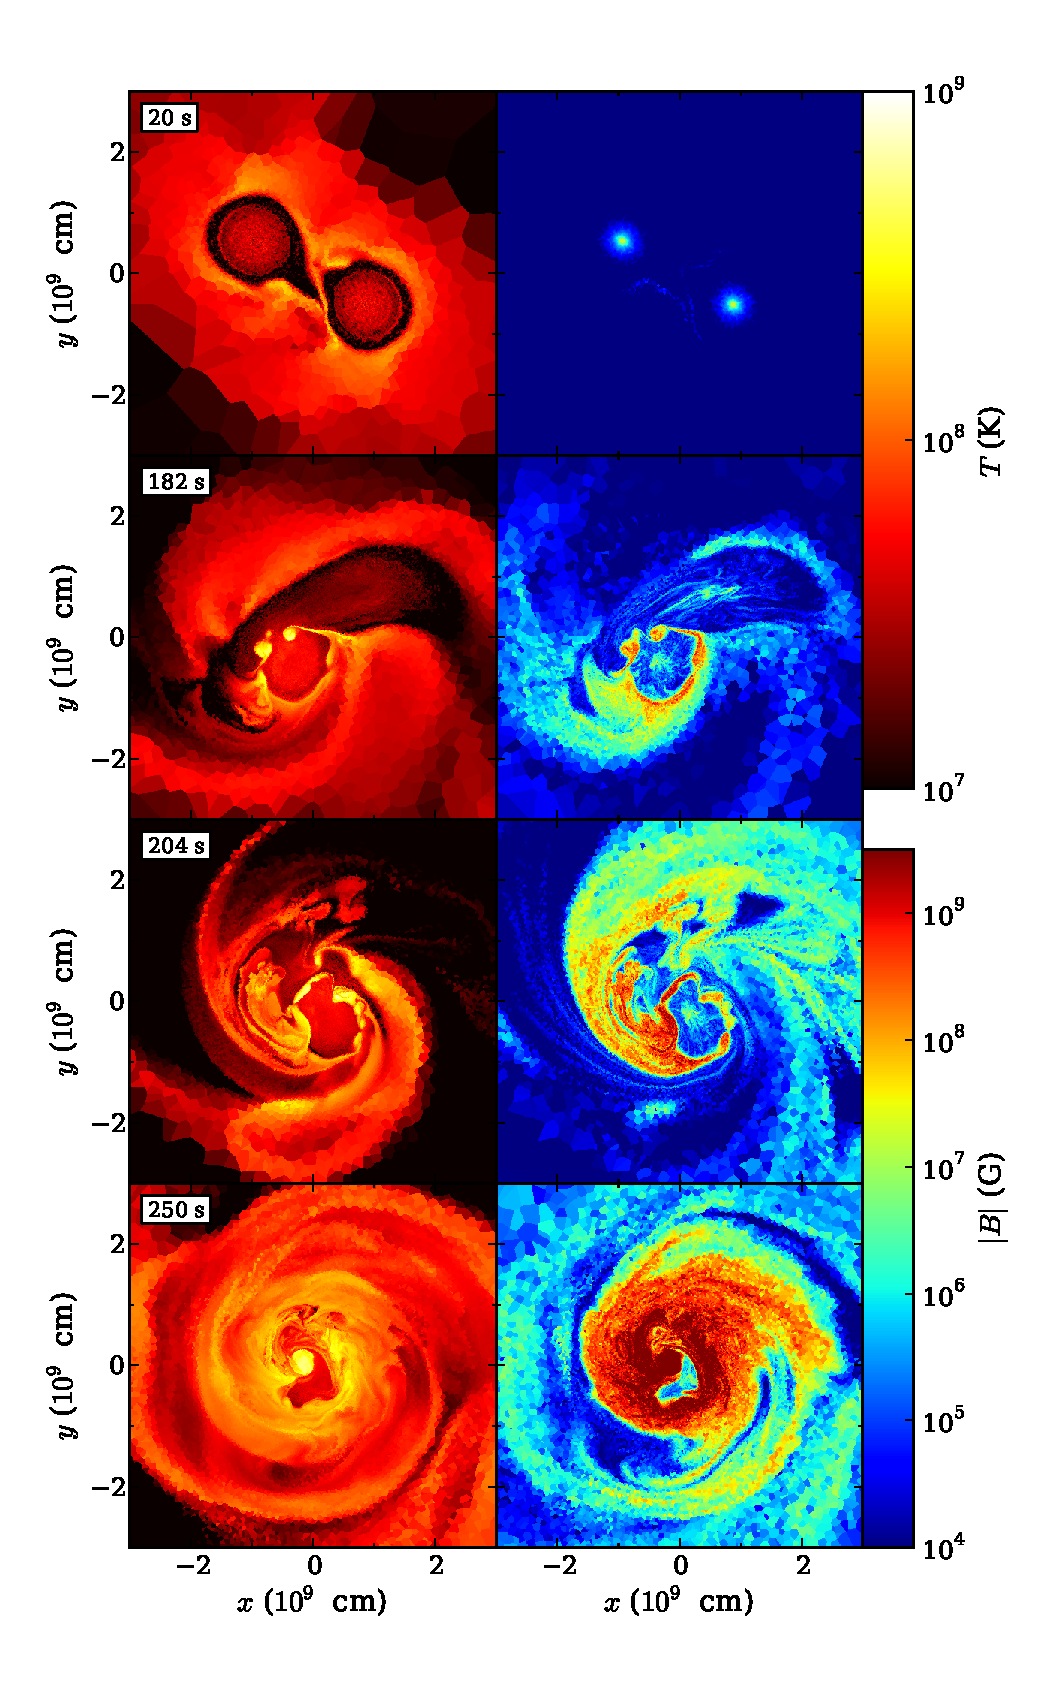
\includegraphics[angle=0,width=0.8\columnwidth]{chapter4_zhu+15/figures/snapshots.pdf}
\caption{Series of temperature $T$ (left column) and magnetic field strength \Bmag\ (right) logarithmic intensity profiles in the equatorial plane of the merger for four snapshots in time (rows; time indicated at the top left of each row).}
\label{fig:c4_snapshots}
\end{figure}

\begin{figure}
\centering
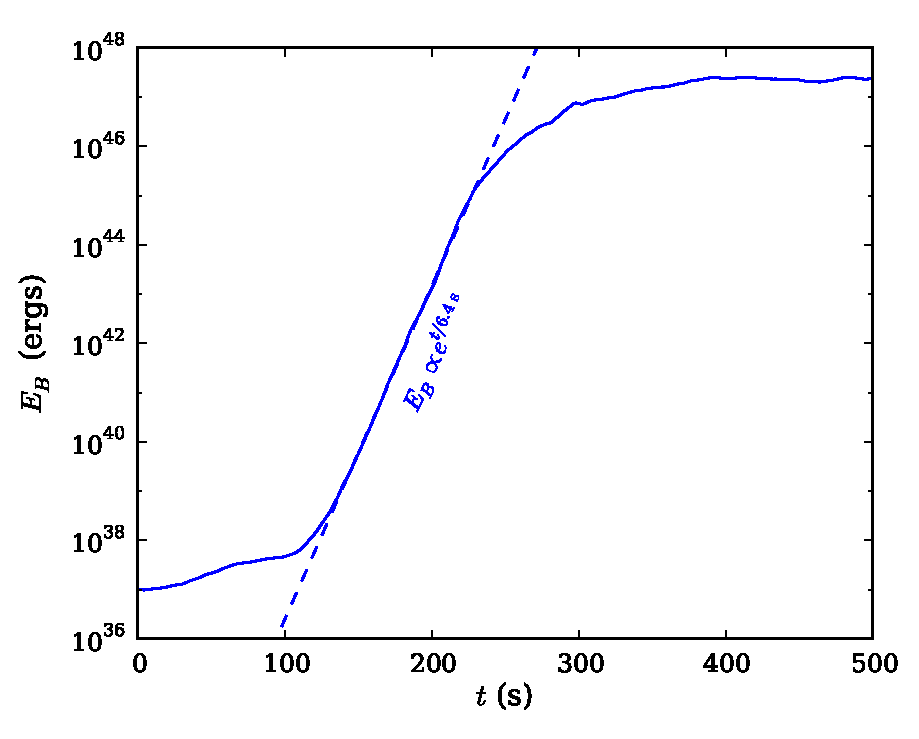
\includegraphics[angle=0,width=0.7\columnwidth]{chapter4_zhu+15/figures/bgrowth.pdf}
\caption{Total magnetic energy \EB\ over time, with a best fit to the rapid exponential growth (dashed $\EB \propto e^{t/6.4\,\mrm{s}}$ line).}
\label{fig:c4_bgrowth}
\end{figure}

We depict the evolution of the binary in Fig. \ref{fig:c4_snapshots}, highlighting temperature $T$ and magnetic field strength \Bmag.  Fig. \ref{fig:c4_bgrowth} shows the growth of total magnetic energy \EB\ over time.

In the first stage of the merger, up to $\sim180$ s, the 0.625 \Msun\ donor WD transfers mass to the 0.65 \Msun\ accretor for about 3.5 orbits before fully disrupting.  Because our initial conditions are approximate -- the WDs are not initially tidally deformed -- mass transfer begins in spurts as the WDs stretch in response to the binary potential, and occurs at a rate that is artificially high \citep{dan+11}.  The early mass transfer shears the atmospheres of both WDs.  As a result, \EB\ grows roughly linearly in the first $\sim100$ s, reaching about quadruple its initial value.  Since the initial mass transfer rate is artificially high, this growth is likely an overestimate, but remains negligible compared to what follows.

%\EB\ could also be a very shallow exponential - the linear fit is marginally better

By $\sim120$ s, mass transfer becomes steady, and a stream of material from the donor wraps around the accretor, forming a shear layer.  Along it, the Kelvin-Helmholtz instability generates a string of hot vortices that exponentially amplify their entrained magnetic fields.  This is illustrated in Fig. \ref{fig:c4_snapshots} (row 2), where the hot vortices along the donor-accretor interface correspond to regions of high field strength.  At $\sim180$ s, tidal forces between the two WDs become strong enough to fully disrupt the donor, which then coalesces with the accretor over $\sim50$ s.  During this time, infalling donor material spirals into the accretor, severely deforming the accretor while carrying the string of magnetized vortices toward the system's center of mass (CM).  Fig. \ref{fig:c4_bgrowth} shows \EB\ growing exponentially by a factor of $\sim10^7$ over $\sim100$ s, with an $e$-folding time $\tau = 6.4$ s, comparable to the typical turnover timescale of the largest eddies $2\pi R_\mrm{eddy}/\Delta v_\mrm{shear} \sim 3\,\mrm{s}$, where $\Delta v_\mrm{shear}$ is the velocity difference across the shear layer.

%2\pi/\Omega_\mrm{eddy} approximated using the three largest eddies in snapshot_092 with 2*pi*r_eddy/v_eddy; r_eddy ~ 1e8 cm, v_eddy ~ 2e8 cm/s.  Similar (slightly smaller) number achieved by looking at the shear layer thickness and delta v.

By $\sim250$ s many of the vortices have merged together into a hot, rapidly rotating underdense void at the CM (Fig. \ref{fig:c4_snapshots}, row 4).  Magnetic growth within the void begins to saturate as its magnetic and kinetic energy approach equipartition.  The rate of field growth slows as well, with \EB\ growing another two orders of magnitude over $\sim150$ s before plateauing at $\sim2\times10^{47}$ ergs at $\sim400$ s.

%Time-averaged E_B between 400 - 500 s to get equilibrium value

\begin{figure}
\centering
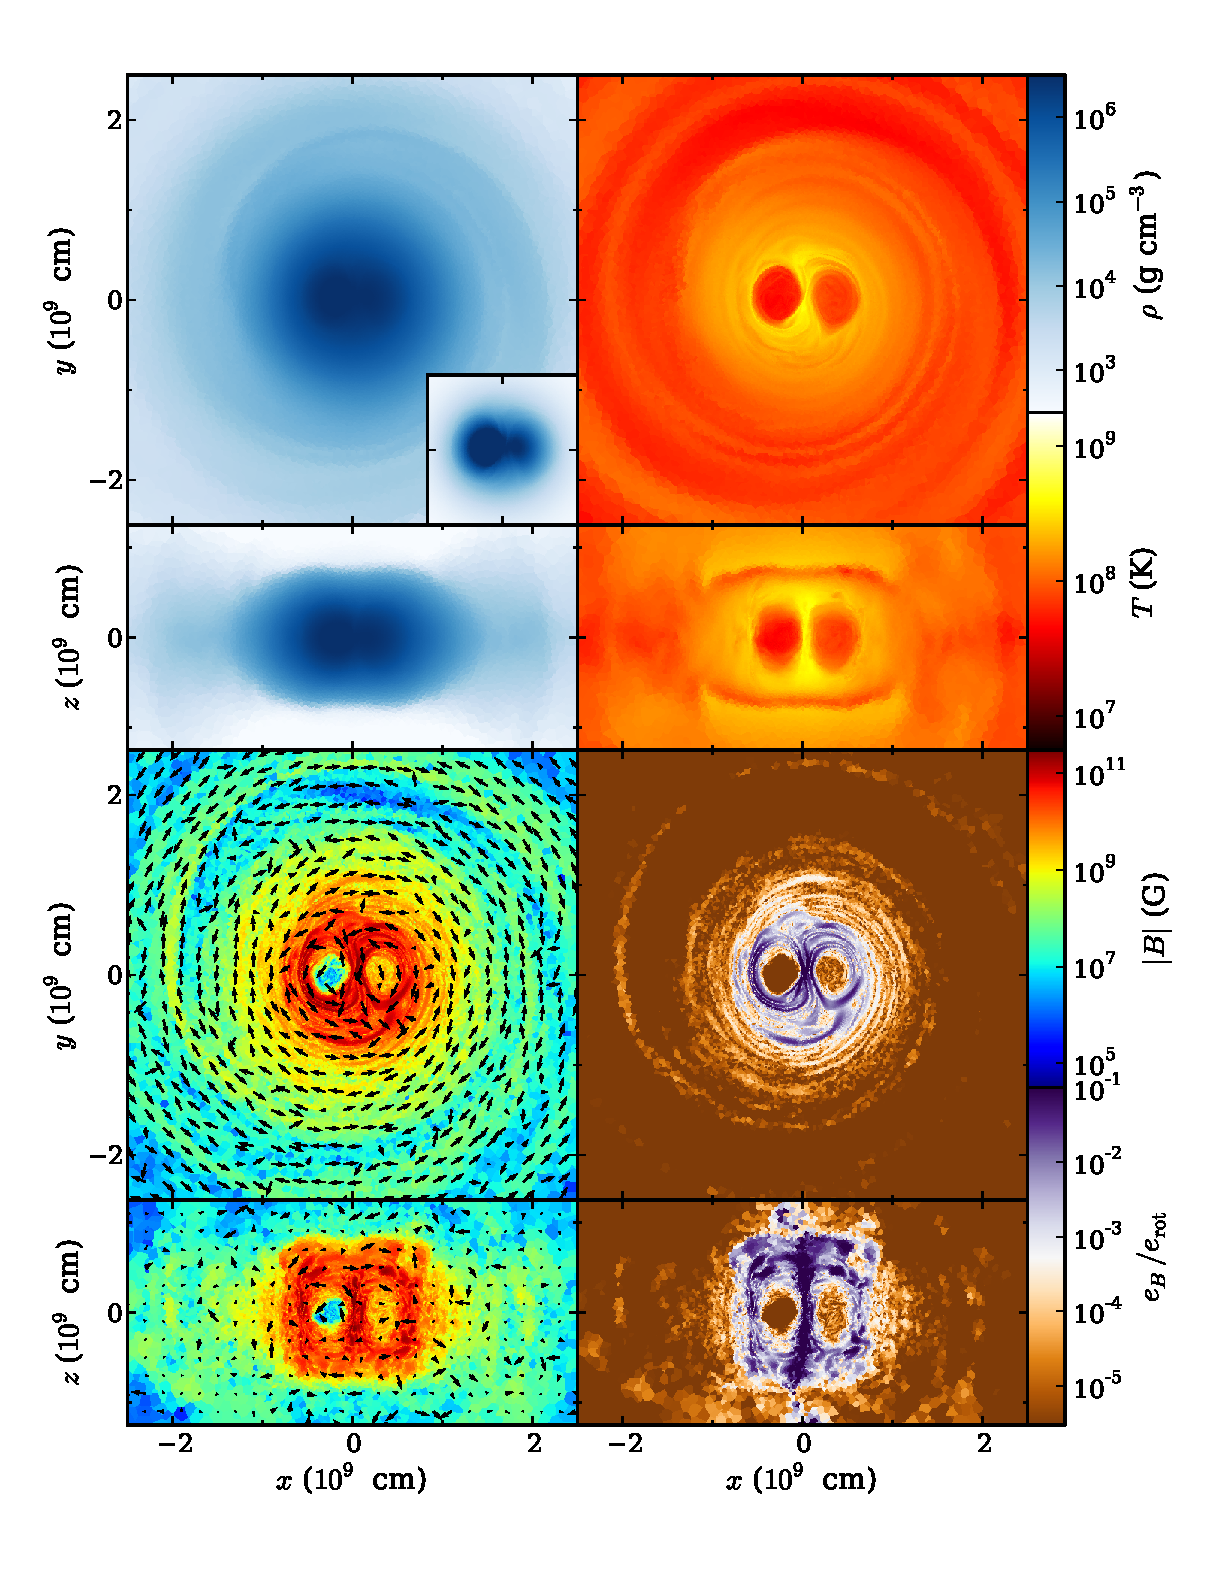
\includegraphics[angle=0,width=0.9\columnwidth]{chapter4_zhu+15/figures/remnant.pdf}
\caption{From leftmost to rightmost column, equatorial plane (top row) and polar (bottom) logarithmic intensity profiles of density $\rho$, temperature $T$, magnetic field strength \Bmag\ and ratio of magnetic to rotational energy density \eberot\ for the simulation at 400 s ($\sim170$ s after coalescence).  The equatorial plane density plot includes a linear profile of the remnant core (with the same $x$ and $y$ scale as the logarithmic profile) to show its shape.  Arrows in the magnetic field strength plots indicate field directions, with their lengths equal to the fraction of the field that lies along the $xy$ plane (top frame) and $xz$ plane (bottom).}
\label{fig:c4_remnant}
\end{figure}

%The core is defined as e_deg/e_tot >= 0.5.  The core essentially consists of all material below r = 7e8 cm, including material at ~3e5 g/cm^3.

In Fig. \ref{fig:c4_remnant} we show the density $\rho$, $T$, \Bmag\ and ratio of magnetic to rotational energy density \eberot\ of the merger remnant at 400 s.  The remnant consists of a dense, degeneracy-supported core containing $\sim60$\% of the remnant's mass, a partly thermally supported hot envelope that surrounds the core, and a rotationally supported disk, a configuration similar to the SPH 0.625-0.65 \Msun\ remnant from Ch. \ref{ch:ch2}.  The \arepo\ remnant core, however, has distinctly non-axisymmetric density and temperature structures, unlike the SPH simulation which achieves axisymmetry $\sim170$ s after coalescence (\citealt{zhu+13}, online figure set Fig. 1.16).  The magnetic fields are too weak during the merger to have an effect on merger dynamics, so these contrasts are due to differences in the \textit{hydrodynamic} schemes between \arepo\ and SPH (Ch. \ref{ch:ch3}).

%From data used in Z13, 2.5% non-axisymmetry is achieved at ~270 s (frame 54000), while coalescence finishes at ~100 s.

%We find running the \arepo\ simulation without any magnetic field still produces a remnant with density and temperature structures similar to those in Fig. \ref{fig:c4_remnant}, and so magnetic fields have a negligible effect on the dynamics of the merger.  Contrasts between the SPH and \arepo\ simulations are due to differences in the \textit{hydrodynamic} schemes between \arepo\ and SPH \Zhuprep.

The remnant magnetic field configuration is complex: while field lines are coherent along ``strands'' of high field strength, neighboring strands often point in opposite directions (see Fig. \ref{fig:c4_remnant}).  In the core, the volume-averaged field strength is $4\times10^{10}$ G, but strands of $>10^{11}$ G field perforate the core.  The field remains $>10^9$ G near the core-disk interface at $\sim 10^9$ cm, before dropping below $10^7$ G at $\gtrsim 3\times10^9$ cm.  The total magnetic field energy is $\sim0.2$\% the total, $\sim0.6$\% the total rotational, and $\sim6$\% the total differential rotation energy of the remnant.\footnote{Differential rotation energy of a cell is estimated with $E_\mrm{drot} = m_\mrm{cell}|\boldsymbol{v}||\nabla\times\boldsymbol{v}|V_\mrm{cell}^{1/3}$.}  This energy is roughly equally partitioned into toroidal and poloidal field components, with the ratio of poloidal to total magnetic energy $\EBphiEB = 0.62$.  Studies of local field amplification within Kelvin-Helmholtz vortices predict magnetic growth saturates when the magnetic and kinetic energy densities are close to equipartition \citep{oberam10, zrakm13}.  In our simulation, this is only the case for the strands of $>10^{11}$ G field, where magnetic energy density is $\sim7$\% ($\sim47$\%) the rotational (differential rotation) energy density (see Fig. \ref{fig:c4_remnant}, column 4).  It is possible that because the strands are distributed throughout the core, they drive the core's overall evolution and inhibit further magnetic amplification in their surroundings.

%In post-merger magnetic amplification scenarios where a dynamo acts upon the inner disk, the field produced remains confined to the inner disk because the diffusion time into the core, $\sim10^9$ yr, exceeds even the remnant thermal cooling time, $\sim10^{7.5}$ yr \citep{garc+12}.  Our fundamentally different configuration results from strong fields being advected into the core during coalescence.  We note, however, that \Bmag\ remains relatively low in the densest parts of the core, and post-merger evolution may shift these regions toward the center, displacing highly magnetized material in the process.

Some of the magnetized accretion stream is ejected during coalescence and integrates into the inner disk ($\sim1 - 3\times10^9$ cm), producing a $10^7 - 10^8$ G field by 400 s.  This field has a negligible hydrodynamic effect on the disk (magnetic energy density to pressure ratio $e_\mrm{B}/P \approx 3\times10^{-5}$ at $2\times10^9$ cm), and, unlike the field in the core, has \textit{not} saturated: \Bmag\ continues to grow exponentially with $\tau \sim 200$ s.\footnote{The remnant disk is generally poorly resolved, even at the highest resolution used in Sec. \ref{ssec:c4_restest}; this may artificially slow the disk field growth rate.}

\section{Robustness Tests}
\label{sec:c4_robust}

\begin{figure}
\centering
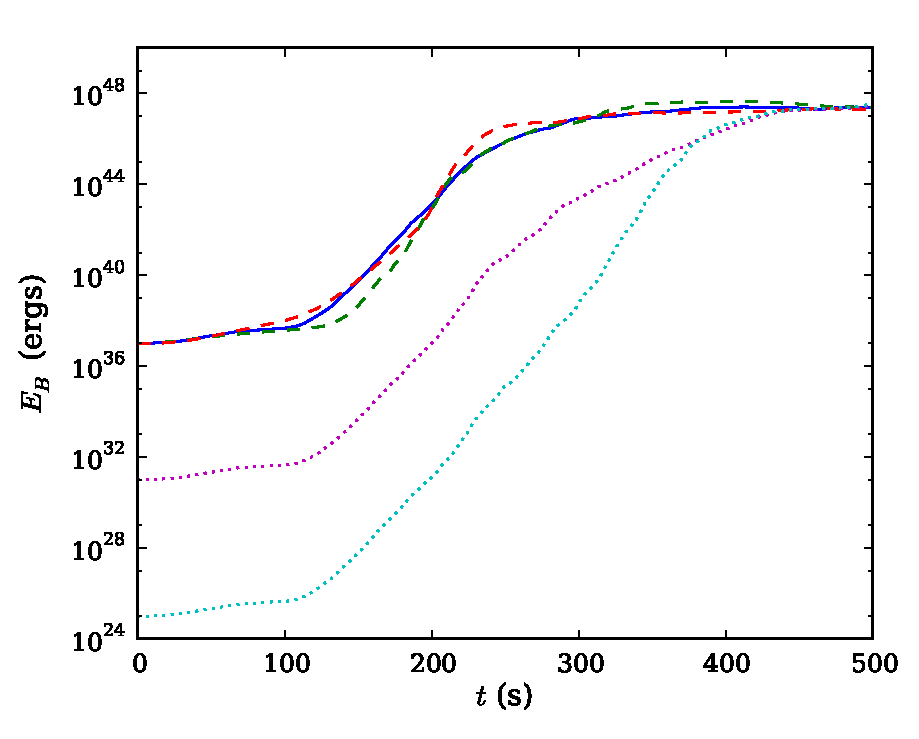
\includegraphics[angle=0,width=0.7\columnwidth]{chapter4_zhu+15/figures/bcomp.pdf}
\caption{Total magnetic energy \EB\ over time for the fiducial (solid blue; $m_\mathrm{cell} \approx 1\times10^{-6}$ \Msun, equatorial surface field strength $10^3$ G) simulation and the robustness tests.  Dashed lines represent low (green; $m_\mathrm{cell} \approx 5\times10^{-6}$ \Msun) and high resolution (red; $m_\mathrm{cell} \approx 2\times10^{-7}$ \Msun) simulations.  Dotted lines represent $1$ G (magenta) and $10^{-3}$ G (cyan) low initial field simulations.}
\label{fig:c4_bcomp}
\end{figure}

\subsection{Resolution Test}
\label{ssec:c4_restest}

To check that our results are not resolution-limited, we performed simulations, otherwise identical to the fiducial one in Sec. \ref{sec:c4_results}, with lower and higher mass resolutions of $m_\mathrm{cell} \approx 5\times10^{-6}$ \Msun\ and $m_\mathrm{cell} \approx 2\times10^{-7}$ \Msun, respectively.  Fig. \ref{fig:c4_bcomp} compares the \EB\ evolution between these simulations (dashed lines) and the fiducial one (solid).

The three runs are qualitatively identical.  Donor disruption and the start of exponential field growth occurs $\sim0.75$ orbital periods earlier at low resolution, and $\sim0.5$ periods later at high, because the outer layers of the WDs are better captured and the differences in hydrostatic equilibrium between \arepo\ and \gasoline\ are less pronounced at higher resolution.  Exponential growth rates are similar between the runs - the \EB\ $e$-folding time is $\tau = 4.9$ s for the low resolution run, faster than $\tau = 6.4$ s for the fiducial.  At high resolution, the growth curve appears to be separated into two phases, with $\tau = 7.8$ s before coalescence, and $\tau = 3.9$ s during it.  The total magnetic energy at the end of exponential growth is also similar - at 400 s, \EB\ is $\sim4\times10^{47}$ ergs in the low resolution run and $\sim1.5\times10^{47}$ ergs in the high, compared to $\sim2\times10^{47}$ ergs at the fiducial resolution.  The fiducial and high resolution runs also qualitatively have very similar magnetic field structures by 400 s.  Our fiducial resolution of $1\times10^{-6}$ \Msun\ therefore appears sufficient for qualitatively capturing the growth and final field configuration of the merger.

In their MHD disk galaxy simulations, \cite{pakms13} find faster field growth and higher field strength at saturation in their lowest resolution run, which they attribute to larger divergence errors at lower resolution.  We perform a similar test, and also see a trend of decreasing divergence error (and more accurate magnetic evolution) at higher resolution, though the errors of all our simulations are at least a factor of two smaller than any reported in \cite{pakms13}.  The errors are highly localized in space and trace steep magnetic gradients, suggesting they contribute only to small-scale variations in the magnetic field.

%In their MHD disk galaxy simulations, \cite{pakms13} find faster field growth and higher field strength at saturation in their lowest resolution run, which they attribute to larger divergence errors at lower resolution.  Performing a similar test, we find the time-averaged \divBrat\ (\divBratnorm) to be $-9.6\times10^{-4}$ ($1.9\times10^{-1}$) for the low resolution, $2.0\times10^{-4}$ ($1.4\times10^{-1}$) for the fiducial, and $7.7\times10^{-5}$ ($1.0\times10^{-1}$) for the high resolution run.  As expected, we see a trend of decreasing divergence error (and more accurate magnetic evolution) at higher resolution, but we note that the errors of all our simulations are at least a factor of two smaller than any reported in \cite{pakms13}.  The errors are highly localized in space and trace steep magnetic gradients, suggesting they contribute only to small-scale variations in the magnetic field.

\subsection{Changing the Seed Field Strength}
\label{ssec:c4_seed}

To understand the dependence of our results on the initial seed field, we ran two additional simulations in which we decreased the strength of the seed field by $3$ and $6$ orders of magnitude leading to an initial equatorial surface field of $1$ G (central field $\sim2\times10^{4}$ G), and $10^{-3}$ G ($\sim20$ G), respectively.  Fig. \ref{fig:c4_bcomp} shows their \EB\ evolution (dotted lines).  We find the growth curves to be homologous between both low initial field runs and the fiducial one -- differing only by the ratios of seed \EB\ -- up to $\sim200$ s, with the $e$-folding time for exponential amplification approximately $6.5$ s for all three runs.  By $\sim250$ s, the field in the fiducial simulation begins to plateau, while amplification (of initially weaker fields) continues for several hundred more seconds in the low initial field runs.  For both runs, \EB\ plateaus at $\sim3\times10^{47}$ ergs, comparable to the fiducial $\sim2\times10^{47}$ ergs.  Because the fields in the low initial field runs remain dynamically irrelevant for longer, however, their structures differ from that of the fiducial run and resemble more the crescent in Fig. \ref{fig:c4_snapshots}, row 4.  The disk field does not saturate in any simulation -- its strength is proportional to the strength of the seed field, and is thus much weaker in the low initial field runs.  Our tests thus suggest that the exponential growth, growth timescale and plateau \EB\ are robust to changes in initial field strength, while the remnant field configuration is more sensitive to the choice of seed field.

\section{Discussion}
\label{sec:c4_discussion}

We have shown that the merger of a 0.625 - 0.65 \Msun\ CO WD binary produces a strong, $>10^{10}$ G magnetic field with a complex structure that winds through the remnant core and into the inner disk.  Similar to previous simulations of binary NS mergers, the strong field is generated by dynamo action within Kelvin-Helmholtz vortices formed during the coalescence of the two WDs.  Since these vortices are ubiquitous in WD mergers, strong magnetic fields are a likely feature of all merger remnants.  The degree to which a field permeates the remnant core depends on how thoroughly the donor and accretor mix during coalescence, which itself is sensitive to initial conditions such as the degree of synchronization between the WDs, or how accurately their tidal bulges and early mass transfer are captured \citep{dan+11, dan+14}.  A parameter space study of magnetized mergers is needed to investigate the range of possible remnant field configurations.

%The highest-resolution NS merger simulations resolve their stars with $\sim100^3$ grid cells, which is approximately the same resolution we use, and a factor of $10^3$ too small to reach the spatial resolution of local vortex simulations.

We note that NS mergers simulated in Eulerian grid codes generally show \EB\ growing by only a factor of $\sim10^2-10^3$ during coalescence, compared to the $\sim10^9$ we see, despite these simulations having resolutions comparable or superior to our low resolution \arepo\ run.  This weaker growth is also inconsistent with the amplification to local kinetic equipartition seen in small-scale simulations \citep{oberam10, zrakm13}, and is attributed to insufficient resolution in the NS merger simulations (\citealt{kiuc+14,giac+15}, though see \citealt{dionar15}).  \cite{giac+15} incorporated a subgrid magnetic amplification model, calibrated using \cite{zrakm13}'s results, into their Eulerian NS merger simulation, and found \EB\ amplification by a factor of $\sim10^{10}$ over a single dynamical time.\footnote{\cite{pricr06}'s SPH simulations also show strong amplification; while runs using their Euler potential MHD method suffer exaggerated field growth from improper boundary conditions, their $\boldsymbol{B}$-based runs show similar results \citep{pric12}.}  This suggests \arepo\ may be better able to resolve small-scale velocity structures than an Eulerian code at comparable resolution, or better able to couple these structures to magnetic growth.  Further work is needed to understand the magnetic field growth in detail.

The density profile of the remnant remains non-axisymmetric for hundreds of seconds after coalescence.  As a result, the core continues to evolve dynamically, and by 400 s has begun to launch a pair of spiral waves into the surrounding medium (see the density panel of Fig. \ref{fig:c4_remnant}), which transport angular momentum on a timescale rivalling that for magnetic shear.  While \cite{kash+15} report a similar spiral instability in their Eulerian remnant evolution simulation, SPH simulations like those of Ch. \ref{ch:ch2} rapidly achieve axisymmetry after coalescence and do not form spiral waves.  As noted earlier, this difference between \arepo\ and SPH simulations is a product of the differences between their hydrodynamic schemes.  Further study is needed to understand these differences and their consequences for remnant evolution (Ch. \ref{ch:ch3}).

%While \cite{schw+12} use an $\alpha$-viscosity to emulate magnetic viscosity

The post-merger evolution of the remnant has been followed to $\sim3\times10^4$ s with axisymmetric cylindrical (two-dimensional) Eulerian grid simulations \citep{schw+12,ji+13}.  As described earlier, \cite{ji+13}'s MHD simulation of a 0.6 - 0.6 \Msun\ remnant shows the development of a strong magnetic field due to MRI.  The subsequent heating and angular momentum transport due to the fields pushes core temperatures to ignition, supporting the possibility of a nuclear runaway within sub-\Mch\ remnants.  Their results are, however, likely sensitive both to their initial hydrodynamic conditions -- which may have artificially high core temperatures -- and their chosen seed magnetic field, a pure poloidal one to optimize the onset of MRI.  Our much stronger poloidal-toroidal field could substantially change post-merger evolution.  Moreover, the persistence of a non-axisymmetric remnant core will lead to evolution that clearly cannot be captured in a axisymmetric cylindrical grid.  We therefore stress the need to perform high-resolution three-dimensional simulations of post-merger evolution to determine the final fate of the remnant.

%Schwab et al. doesn't make any mention of a jet, though in our old 2D PME simulations we did find one with only an alpha viscosity installed (those sims aren't to be trusted though).  Their outflow is also limited to < 10^-5 Msun.

There are a number of potentially observable consequences of the magnetic fields produced by the merger.  \cite{ji+13} note the creation of a magnetized corona and biconal jet in their simulations, which act in concert to cause an outflow of material near the remnant's poles.  This outflow eventually unbinds $\sim10^{-3}$ \Msun\ of material, and \cite{belo14} estimates it should lead to an optical transient with a duration of $\sim1$ day and peak $L \sim10^{8}$ \Lsun, which should be detectable by optical surveys.

If a remnant later experiences a nuclear runaway and explodes as a SN Ia, its magnetic field will increase the late-time emission by trapping positrons (produced by $^{56}$Co $\beta^+$ decay) that would otherwise escape the ejecta.  The trapping efficiency depends on the strength and configuration of the remnant magnetic field, with a locally entangled $\sim10^{11}$ G field -- similar to our findings -- well able to trap positrons past 1000 days \citep{ruizs98}.  This is in line with observed late-time SN Ia light curves (most recently \citealt{kerz+14}).

Those remnants that do not explode will retain strong fields when they reach quiescence, and populate the high-mass tail of the distribution of isolated high-field magnetic WDs \citep{garc+12,kule+13,wicktf14,brig+15}.  Since these remnants will have temperatures high enough to fuse any remaining hydrogen and helium they possess, their properties might eventually be akin to the recently discovered hot DQ WDs (e.g. \citealt{dufo+13}).  These WDs have carbon-dominated atmospheres and $T_\mrm{eff} \approx 2\times10^4$ K, are often strongly magnetized ($\sim1$ MG) and sometimes have monoperiodic photometric variability (possibly due to rapid rotation).  Their origins remain unclear \citep{alth+09, lawr+13, will+13}.  \cite{dunlc15} recently found that, if most known hot DQs are massive ($M \gtrsim 0.95\Msun$), their population's velocity dispersion corresponds to a kinematic age much older than what would be inferred from their temperatures, suggesting that at least some hot DQs are WD-WD merger remnants.  If so, their observed properties would constrain merger and remnant evolutionary models, and double-degenerate channels for SNe Ia.

\vspace{5mm}

We thank Christopher Thompson, Christopher Matzner, Volker Springel, Bart Dunlap, Yuri Levin, Henk Spruit, Ue-Li Pen and Stephen Ro for their insights into magnetohydrodynamics and simulations.  This work utilized the SciNet HPC Consortium's GPC supercomputer \citep{loke+10}.  C.Z. acknowledges support from the Natural Sciences and Engineering Research Council (NSERC) Vanier Canada Graduate Scholarship.  R.P. acknowledges support by the European Research Council under ERC-StG grant EXAGAL-308037 and by the Klaus Tschira Foundation.  P.C. is supported by the NASA ATP program through NASA grant NNX13AH43G, and NSF grant AST-1255469.  

\section{Postscript: Reconsidering Divergence Cleaning in \arepo}
\label{sec:c4_postscript}

In Sec. \ref{sec:c4_discussion} we discussed why \arepo\ might be capturing (at least some proxy of) rapid magnetic amplification during the merger when Eulerian simulations of NS mergers at similar resolutions do not.  Since the publication of Ch. \ref{ch:ch4} as \cite{zhu+15}, it has been pointed out that the amplification could be the spurious result of \arepo's divergence cleaning mechanism.

%The MHD equations of motion (Eqn. \ref{eqn:c3_mhd_eqns}) do not contain $\bf{\nabla\cdot B}$, since they are identically zero according to Maxwell's Equations.

In most multidimensional numerical MHD schemes, the ``divergence constraint'' of $\bf{\nabla\cdot B} = 0$ is not guaranteed, and if the implicit divergence terms in Eqn. \ref{eqn:c3_mhd_eqns} are not considered, these schemes can in practice lead to spurious forces and magnetic instabilities \citep{toth00, hopkr16}.  A number of solutions exist (eg. \citealt{toth00}), and the most widely-used is \cite{evanh88}'s constrained transport method, which staggers the different components of the magnetic field within the discretization to maintain the divergence constraint to round-off errors.  This reliance on grid geometry, however, has made it challenging to implement in a moving mesh code \citep{moczvh14}.  Until the recent adoption of constrained transport in \arepo\ in \citep{mocz+16}, the code instead used either the \cite{dedn+02} or \cite{powe+99} divergence control schemes.  The former introduces an additional conserved scalar term $\psi$ to ${\bf U}$ in Eqn. \ref{eqn:c3_mhd_eqns_compact} which is coupled to $\bf{\nabla\cdot B}$ while simultaneously being advected and forced to exponentially decay.  The latter adds a source term to the righthand side of Eqn. \ref{eqn:c3_mhd_eqns_compact} that is proportional to $\bf{\nabla\cdot B}$, which passively advects divergence errors but does not damp them.  The Dedner method is superior because it actively minimizes divergence errors rather than simply preventing their local accumulation, but its implementation in \arepo\ required prohibitively small timesteps and tended to become unstable in highly dynamic environments \citep{pakms13}, hence our use of the Powell scheme.

% DEFENCE NOTE: CT actually keeps the divergence constant, making it only necessary to initialize the simulation with $\bf{\nabla\cdot B} = 0$; see \citealt{toth00}, Sec. 4.1

% DEFENSE NOTE: if the implicit divergence terms in Eqn. \ref{eqn:c3_mhd_eqns} are not considered, these schemes can in practice lead to spurious forces and magnetic instabilities that do not become negligible even at infinite resolution

% DEFENSE NOTE: Pakmor+11 uses the GLM-MHD method, though I find Eqn. 10 of Hopkins and Eqn. 24 of Dedner+02 to be the cleanest representations of this method.  Note that \psi is not proportional to B, but rather just coupled to it - see Eqn. 5 of Dedner, and the explanation around Eqn. 18, which shows that \psi in general has parabolic and hyperbolic (exponentially decreasing) components, leading to both exponential damping as well as transport via waves.

\begin{figure}
\centering
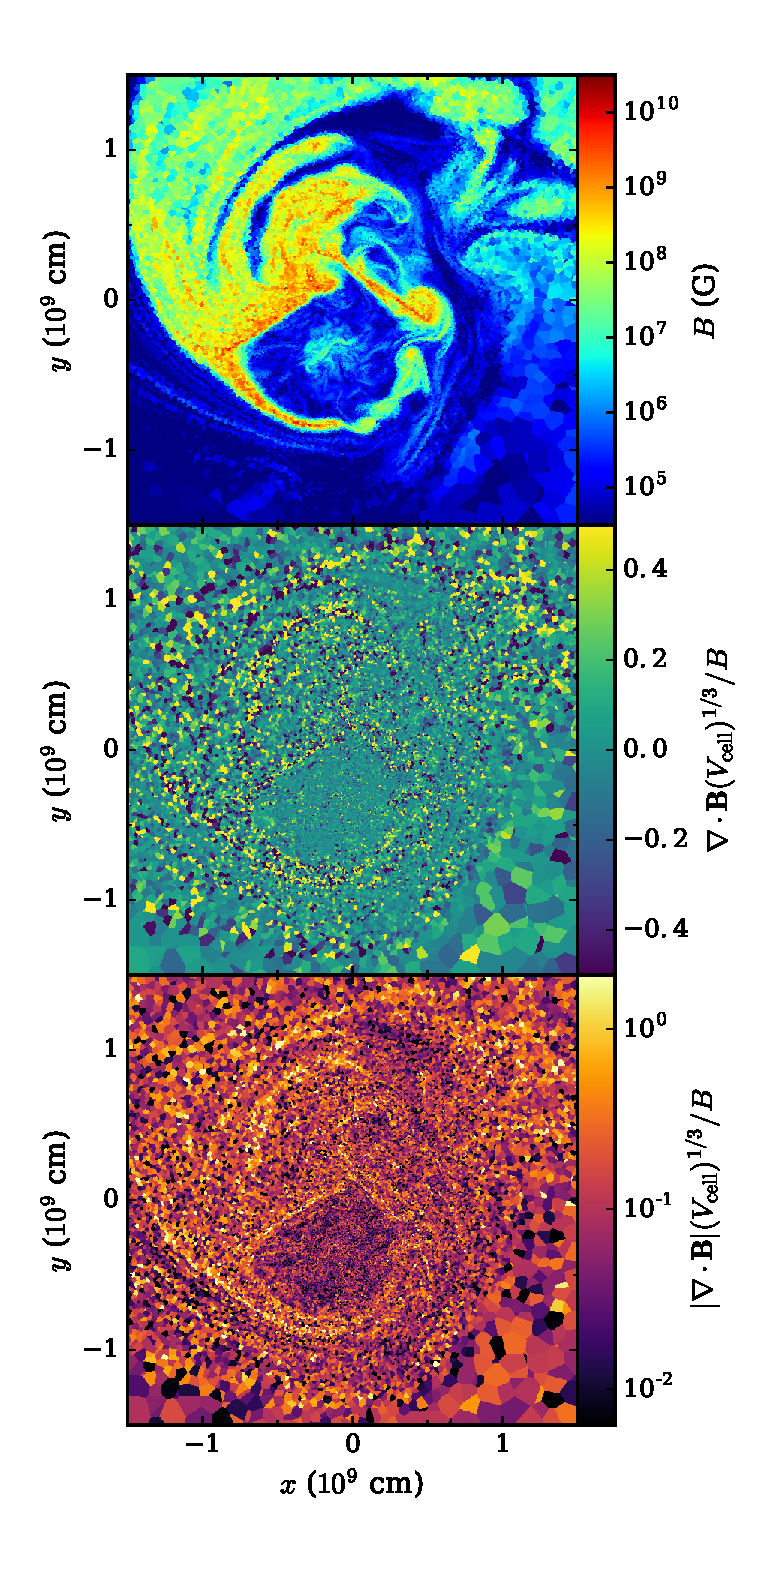
\includegraphics[angle=0,width=0.6\columnwidth]{chapter4_zhu+15/figures/bdiv.pdf}
\caption{From top to bottom, equatorial plane intensity profiles for the magnetic field strength, relative divergence error (linear scale) and absolute relative divergence error (logarithmic) for the simulation at $200\,\mrm{s}$.}
\label{fig:c4_bdiv}
\end{figure}

In Fig. \ref{fig:c4_bdiv}, we show the magnetic field strength, relative divergence error and absolute relative divergence error of our fiducial merger simulation at $t = 200\,\mrm{s}$, when the donor has just been disrupted.  The (mass-weighted) average relative divergence error $\left\langle|\mathbf{\nabla\cdot B}|(V_\mrm{cell})^{1/3}/B\right\rangle = 0.18$ (where $V_\mrm{cell}$ is the Voronoi cell volume) is typical of both this simulation and \cite{pakms13}'s galaxy disk evolution one, but much larger than typical results from Dedner cleaning-based codes \citep{tric15, hopkr16}.  As in \cite{pakms13}, the divergence error alternates on very small scales (Fig. \ref{fig:c4_bdiv} middle panel), and peaks near large magnetic gradients (comparing top and bottom panels).  While errors cancel over large scales (the average relative error with the sign of the divergence included is $\left\langle\mathbf{\nabla\cdot B}(V_\mrm{cell})^{1/3}/B\right\rangle = -1.4\times10^{-3}$), the regions of highest magnetic gradient correspond to the shear interface between donor and accretor, where we believe the field is amplified.  It is therefore plausible that errors at small scales spuriously magnify the magnetic dynamo associated with the shear layer and Kelvin-Helmholtz vortices.  

This hypothesis is supported by \cite{hopkr16}, who perform a battery of tests comparing the Dedner and Powell mechanisms for their mesh-free finite-volume code \textsc{GIZMO}, and show divergence errors in Powell-based simulations of advection and hydromagnetic instability lead to spurious and unstable field growth.  Moreover, comparisons between Powell and constrained transport-based \arepo\ using simulations of MHD turbulence and disk galaxy evolution show that the Powell scheme leads to greater magnetic field amplification by up to an order of magnitude, as well as a qualitatively different field topology \citep{mocz+16}.

%while \cite{pakms13} find good agreement between Powell-based \arepo\ simulations and CT-based Eulerian ones for the Orzag-Tang vortex problem and magneto-rotational instability within a disk

%In Hopkins's most extreme test, SPH returns divergence errors of order 0.1 - 1 (Gizmo 0.01 - 0.1), but Arepo (pakmor+13) gives errors of order unity!

Caution is therefore in order when using this chapter's results, at least until they have been compared with simulations using \arepo's new constrained transport scheme.  Given that the results will likely be different, it may also be useful to conduct a simpler test case of field evolution within a single Kelvin-Helholtz vortex at various resolutions and compare the results with those of \cite{oberam10} and \cite{zrakm13}.  Nevertheless, as discussed in Sec. \ref{sec:c4_results}, the remnant magnetic field's bulk properties following coalescence are physically plausible, and are likely to be more robust than the detailed field configuration.  We use these bulk properties (alongside \cite{ji+13}'s work) when considering magnetic simmering WDs the next chapter.

%\cite{pakmv13} find qualitative differences in their resolution test, which they attribute to large divergence errors artificially accelerating magnetic field growth in their low resolution simulations.  While we find no substantial difference in our test, we also check the divergence errors of our two simulations.  We find the time-averaged $\left\langle(\mrm{div} \vec{B}) r/B\right\rangle$ ($\left\langle|\mrm{div} \vec{B}| r/B\right\rangle$ during coalescence only) to be $1.1\times10^{-4}$ ($1.3\times10^{-1}$) for the fiducial run, and $2.0\times10^{-4}$ ($1.4\times10^{-1}$) for the low resolution run.  These errors are comparable to each other, and much smaller than any reported in \cite{pakmv13}.  Divergence errors are spatially highly localized and trace steep magnetic gradients, suggesting that these errors contribute only to small-scale variations in the magnetic field.  \textbf{Editors: $\left\langle(\mrm{div} \vec{B}) r/B\right\rangle$ begins at an enormous $10^{12}$; Ruediger, why would this be?  Did you see something similar in your simulations?}



%%ch5
\chapter{The Evolution of Simmering Sub-Chandrasekhar Mass WDs}
\label{ch:ch5}

\begin{center}
\begin{minipage}[c]{4.75in}
Chenchong Zhu, Philip Chang and Marten H. van Kerkwijk\\
In preparation
\vspace{2em}
\end{minipage}
\end{center}

When fusion is lit in the degenerate interior of a carbon-oxygen white dwarf, the resulting nuclear runaway starts with a ``simmering phase'', in which convection transports energy out of the burning region.  While simmering inevitably leads to some form of explosion for white dwarfs near the Chandrasekhar mass, in ones with lower mass it may instead lead to the lifting of degeneracy and expansion into a carbon-burning star.  Using analytical arguments and simple models, we determine that the critical mass for explosions to be possible is $\Mcrit = 1.135\,\Msun$.  In principle, effects from rotation and magnetic fields might lead to a change in the critical mass.  For the rotation rates found in merger remnant simulations, the effect is almost certainly minimal, $\lesssim0.01\,\Msun$.  For magnetic fields the case is less clear, since interaction with convection is poorly understood, but simple order-of-magnitude arguments again suggests only a small effect.

\section{Introduction}
\label{sec:c5_intro}

Type Ia supernovae (SNe Ia) are generally thought to be the thermonuclear explosions of carbon-oxygen white dwarfs (CO WDs).  While the current body of observational evidence has greatly strengthened this hypothesis, the mechanism(s) by which a WD is agitated into exploding remains mysterious (see \citealt{howe11, hill+13, maozmn14} for recent reviews).  

The traditional scenario involves slow accretion of material onto the CO WD from either a non-degenerate companion or another WD.  As the CO WD approaches the Chandrasekhar mass \Mch, its central density becomes sufficiently high that the rate of heating from pycnonuclear carbon fusion exceeds that of neutrino cooling.  The resulting increase in central entropy establishes a convection zone that transports the heat of the nuclear burning region to the rest of the WD interior.  The WD is highly degenerate, however, and does not expand in response to the heating.  Instead, a nuclear runaway ensues over the next thousand years as the WD grows ever hotter, a period of evolution referred to as the simmering phase.  Near-\Mch\ WDs eventually become hot enough that the timescale for nuclear burning becomes shorter than the dynamical time -- we call this ``dynamical burning'' -- at which point an explosion becomes inevitable.

This scenario is beset by two major issues: an apparent paucity of accreting or merging CO WDs that can achieve \Mch, and the difficulty for the thermonuclear explosion of a \Mch\ WD to reproduce the properties and population-level trends of observed SN Ia (\citealt{vkercj10}, henceforth \citeal{vkercj10}, and references therein).  These, in turn, have spurred research into alternative formation channels where CO WDs with masses significantly \textit{below} \Mch\ also explode.  Including them would bolster substantially the number of progenitors (eg. \citealt{badem12}), and their explosions could closely resemble ordinary SNe Ia \citep{shig+92, sim+10}.

Since hydrostatic sub-\Mch\ WDs do not possess central densities high enough for pycnonuclear fusion, burning must be prompted either by a shockwave (that immediately triggers dynamical burning), or by heating material to $T\approx6\times10^8\,\mrm{K}$ to induce fusion through high temperatures, rather than high densities.  The former is presumed in eg. the double-detonation (eg. \citealt{fink+07, woosk11}), violent merger (eg. \citealt{pakm+10}) and collision (eg. \citealt{loreig10}) scenarios.  The latter is presumed in the sub-\Mch\ CO WD merger scenario of \citeal{vkercj10}, in which two CO WDs of mass $\sim0.65$ \Msun\ merge, forming a merger remnant that is differentially rotating throughout its structure, and so is suceptible to magnetohydrodynamic instabilities \citep{shen+12, ji+13}.  It subsequently becomes strongly magnetized, leading to outward transport of angular momentum over a viscous timescale of $\sim10^4 - 10^8\,\mrm{s}$ that robs the remnant of its rotational support (\citeal{vkercj10}, \citealt{shen+12}; though see Ch. \ref{ch:ch3}, \citealt{kash+15} for evidence of transport through spiral hydrodynamic waves).  This viscous evolution compresses and adiabatically heats the remnant's interior, which the simulation of \cite{ji+13} suggests leads to central carbon ignition.

In the \citeal{vkercj10} scenario, and, indeed, any situation where non-dynamical nuclear burning ignites under degenerate conditions in a sub-\Mch\ WD, a simmering phase ensues just like in the near-\Mch\ case.  Sub-\Mch WDs, however, are less dense, and their degeneracy is at least partially lifted before they reach temperatures where burning becomes dynamical, which depends only weakly on density.  There is, in fact, a critical mass \Mcrit\ below which the simmering WD never reaches dynamical burning before becoming non-degenerate enough to expand and cool off.  Even those WDs that do achieve dynamical burning may substantially expand beforehand.  Since the fraction of material fused to peak-iron products in an SN Ia depends on its progenitor's density profile, a pre-expanded WD will produce reduced, or even negligible, amounts of \Ni.  Thus a nuclear runaway at the center of a sub-\Mch\ remnant neither inevitably leads to an explosion, nor is any explosion guaranteed to resemble an SN Ia.

In this chapter, we investigate the simmering phase of sub-\Mch\ WDs undergoing a center-lit thermonuclear runaway.  In Section \ref{sec:c5_modelsim} we detail our semi-analytical model and its assumptions.  While our motivation is to better understand the evolution of merger remnants, we keep these assumptions simple, and we stress that our models do \textit{not} necessarily account for any specific prior evolution.  We present our results in Section \ref{sec:c5_results}, determining both the value of \Mcrit\ and estimating the mass of radioactive \Ni\ produced if a detonation were to follow immediately.  Simmering WDs that formed in mergers are expected to be rotating and magnetized (eg. Ch. \ref{ch:ch4}, \citealt{wicktf14}), and we also try to ascertain how \Mcrit\ and \MNi\ change in their presence using simple prescriptions for rotational and magnetic convective suppression.  Lastly, in Section \ref{sec:c5_discussion}, we discuss how our results apply to the \citeal{vkercj10} scenario as well as implications for SN Ia progenitor studies in general.

\section{Modeling Sub-\Mch WD Simmering}
\label{sec:c5_modelsim}

Simmering in near-\Mch\ WDs has been extensively studied with 1D semi-analytical calculations by eg. \citeauthor{wooswk04} (\citeyear{wooswk04}; hereafter \citeal{wooswk04}), \cite{lesa+06, piro08}, and \citeauthor{piroc08}; (\citeyear{piroc08}; hereafter \citeal{piroc08}).  We adapt the analytical machinery of \citeal{wooswk04} Sec. 2 and \citeal{piroc08} to sub-\Mch\ WDs.  In Sec. \ref{ssec:c5_simmer} we show that the simmering phase can be approximated well by a sequence of hydrostatic WD models, and in Sec. \ref{ssec:c5_numericalmodels} we detail our model implementation.

\subsection{Analytical Description}
\label{ssec:c5_simmer}

%as well as full 3D hydrodynamic simulations \citep{kuhlwg06, zing+09, zing+11, nona+12}

For a center-lit nuclear runaway, carbon ignition is achieved when material near the center of the WD is heated past $\sim 6 \times10^8\,\mrm{K}$ and the heating timescale due to carbon fusion (at $\rho \sim 10^8\,\gcc$),

\eqbegin
\taucc \equiv \frac{c_PT}{\epscc}\,\sim\,10^2\,\mrm{yr},
\label{eq:c5_taucc}
\eqend

\noindent becomes smaller than the cooling timescale from neutrino losses $\taunu\equiv c_P T/\varepsilon_\nu$.\footnote{The conduction timescale, $\taucond \sim 10^6\,\mrm{yr}$, is far longer than either.}  \epscc\ is the specific energy generation rate for carbon burning, $\varepsilon_\nu$ the specific energy loss rate due to neutrino creation, and $c_P$ the specific heat at constant pressure.  The energy deposited from nuclear burning steepens the temperature gradient until convection is triggered.

%See pg. 260 of Padmanabhan Theoretical Astrophysics Vol. 2 for a derivation of the conduction time.

We now estimate the timescale for convective energy transport, \tauconv, which requires the convective luminosity $\Lconv$.  In steady state convection, this is equal to the nuclear luminosity, i.e.

\eqbegin
\Lconv(r) = \Lcc(r) = \int_0^{r} 4\pi r'^2\rho \epscc(\rho, T)dr'.
\label{eq:c5_convlum}
\eqend

\noindent In a simmering WD part of \Lcc\ is diverted into heating the WD, and to perform work expanding it once degeneracy begins to be lifted, reducing the convective luminosity in the upper convection zone (\citeal{piroc08}).  For simplicity, and because we mainly consider convective velocities near the center of the WD, we do not consider this effect in our models.  

Near the center, and closer to the end of simmering, $\rho_7 = (\rho/10^7\,\gcc) = 3$ and $T_9 = (T/10^9\,\mrm{K}) = 1.2$, and the specific energy generation rate for material composed of $50$\% C and $50$\% O by mass,

\eqbegin
\epscc \approx 1.3\times10^{15} \left(\rho_7/3\right)^{1.3}\left(T_9/1.2\right)^{23.6}\,\mrm{erg}\,\,\mrm{g}^{-1}\,\mrm{s}^{-1}
\label{eq:c5_epsccscaling}
\eqend

\noindent is a steep function of temperature (Eqn. \ref{eq:c5_epsccscaling} was numerically derived using the \texttt{rates} module from the stellar evolution code \mesa\ \citep{paxt+11}).  Thus, the vast majority of the nuclear luminosity is generated within a ``nuclear burning region'' deep within the star.  Following \citeal{wooswk04}, we estimate the burning region's luminosity through the use of a polytropic equation of state and an adiabatic temperature profile -- i.e. $P/P_\mrm{c} = (\rho/\rhoc)^{\gamma_1}$, $T/\Tc = (\rho/\rhoc)^{\gamma_3-1}$.  At $\rho_7 = 3$ and $T_9 = 1.2$, the Helmholtz equation of state (EOS; \citealt{timms00}) gives $\gamma_1 = 1.41$, and $\gamma_3 = 1.43$.  We use the standard polytropic rescaling of density and radius (eg. \citealt{kippww12}): 

\begin{eqnarray}
\theta &\equiv& (\rho/\rho_c)^{\gamma_1 - 1}, \nonumber \\
\xi &\equiv& \alpha r,
\label{eq:c5_poly_def}
\end{eqnarray}

\noindent where

\eqbegin
\alpha \equiv \sqrt{\frac{\gamma_1 - 1}{\gamma_1}\frac{4\pi G\rhoc^2}{P_\mathrm{c}}},
\label{eq:c5_poly_alpha}
\eqend

\noindent along with Eqn. \ref{eq:c5_epsccscaling} to obtain $\rho\epscc(\rho, T) = \rhoc\epscentral\theta^{b - 1}$, where $b = (\gamma_1 - 1)^{-1}(23.6\gamma_3 - 21.3) + 1$ and $\epscentral = \epscc(\rhoc, \Tc)$.  When calculating the total luminosity, Eqn. \ref{eq:c5_convlum} then reduces to

\eqbegin
\Lconv \approx 4\pi\rhoc\epscentral\frac{1}{\alpha^3}\int_0^{\xi_1} \xi^2 \theta^{b - 1} d\xi.
\label{eq:c5_lconvpolytrope}
\eqend

\noindent Close to the WD's center, 

\eqbegin
\theta \approx 1 - \frac{1}{6}\xi^2
\label{eq:c5_theta_approx}
\eqend

\noindent to third order, which implies the integrand of Eqn. \ref{eq:c5_lconvpolytrope} has a maximum at $\xi_1 = \sqrt{6/b}$.  Integrating up to this point numerically,

\begin{eqnarray}
\Lconv &\approx& 0.20\frac{\rhoc\epscentral}{\alpha^3}  \nonumber \\
&=& 2.2\times10^{46}\left(\rho_7/3\right)^{1.3}\left(T_9/1.2\right)^{23.8}\,\mrm{erg}\,\,\mrm{s}^{-1}
\label{eq:c5_convlumred}
\end{eqnarray}

\noindent For the scaling relation above, and for Eqn. \ref{eq:c5_vconvest2} below, we use the Helmholtz EOS to numerically expand $\alpha \approx 7.0\times10^{-9}(\rho_7/3)^{0.33}(T_9/1.2)^{-0.08}\,\mrm{cm}^{-1}$.

%See Chang, White & van Kerkwijk Unpublished Eqns. 10 - 18

The convective velocity \vconv\ transporting luminosity \Lconv\ can be calculated with standard mixing length theory (MLT; eg. \citealt{kippww12} Ch. 7):

\begin{eqnarray}
\Fconv &=& \frac{\Lconv}{4\pi r^2} = \frac{\rho c_PT}{\gacc\delta l_m} \vconv^3 \nonumber \\
\vconv &=& \left(\frac{\delta \gacc l_m}{c_P T}\frac{\Lconv}{4\pi r^2 \rho}\right)^{1/3}.
\label{eq:c5_vconv_mlt}
\end{eqnarray}

%See https://en.wikipedia.org/wiki/Thermal_expansion#Coefficient_of_thermal_expansion for coefficient of thermal expansion = 1/V*dV/dT = -1/rho*drho/dT

\noindent where \gacc\ is the magnitude of the gravitational acceleration, $\delta = -d\ln\rho/d\ln T$ the logarithmic coefficient of thermal expansion and $l_m$ the mixing length, which in this work we shall take to be the pressure scale height

\eqbegin
H_P \equiv -\frac{P}{dP/dr}.
\label{eq:c5_scaleheight}
\eqend

\noindent A coefficient of order a few often included in Eqn. \ref{eq:c5_vconv_mlt} has been set to unity to be consistent with \citeal{piroc08}.  Combining Eqns. \ref{eq:c5_convlumred} and \ref{eq:c5_vconv_mlt}, we estimate the convective velocity at $r = H_P/2$:

\begin{eqnarray}
\vconv &\approx& \left(\frac{e^{\gamma_3/2\gamma_1}}{\pi}\frac{\delta \gacc}{c_P \Tc}\frac{\Lconv}{H_P \rhoc}\right)^{1/3} \nonumber \\
	&\approx& 0.47\left(\frac{\delta \gacc}{\alpha^3H_P}\frac{\epscentral}{c_P \Tc}\right)^{1/3}.
\label{eq:c5_vconvest}
\end{eqnarray}

% m(H_P/2)/H_P^3 approximation below assumes rho = rhoc*exp(-r/(gamma1*H_P)); integrating 4/3*pi*(H_P)^3*rho-bar = 4*pi*rhoc*INT_0^(H_P/2) r^2 exp(-r/(gamma1*H_P)) dr = 4*pi*rhoc*H_P^3*0.0321877 gives us rho-bar = 0.77rhoc \approx rhoc/\sqrt{2}

\noindent Here, we used the fact that $H_P/2$ is the approximate length over which pressure decreases by a factor of $e^{1/2}$; correspondingly (from the adiabatic temperature gradient), $\rho \approx \rhoc\exp(-1/2\gamma_1)$ and $T \approx \Tc\exp(-(\gamma_3 - 1)/2\gamma_1)$.  In the same vein, we relate $\alpha$ to $H_P$ using Eqns. \ref{eq:c5_poly_def} and \ref{eq:c5_theta_approx}:\footnote{The next higher term in the expansion for $\theta$ is $(n/120)\xi^4$, where $n$ is the polytropic index.  Hence, for $n \approx 3$ and $\xi_{H_P} \approx 1.2$, the approximation for $\theta$ is good to $\sim20$\%.}

\begin{eqnarray}
\frac{P}{P_\mathrm{c}} &=& e^{-1} = \theta^{\gamma_1/(\gamma_1 - 1)} \approx \left(1 - \frac{1}{6}\xi_{H_P}^2\right)^{\gamma_1/(\gamma_1 - 1)}  \nonumber \\
\xi_{H_P} &=& \alpha H_P \approx \left(6 - 6e^{-(\gamma_1 - 1)/\gamma_1}\right)^{1/2} = 1.2
\label{eq:c5_poly_xihp2}
\end{eqnarray}

\noindent We also approximate gravitational acceleration $\gacc = Gm/r^2$ ($m$ is the enclosed mass) at $r = H_P/2$ by noting that

\begin{eqnarray}
m\left(H_P/2\right) &=& \int_0^{H_P/2} 4\pi r^2\rho dr \approx 4\pi\frac{\rhoc}{\alpha^3}\int_0^{0.6}\xi^2\theta^{1/(\gamma_1 - 1)}d\xi \nonumber \\
&=& 0.20\frac{4\pi\rhoc}{3\alpha^3} 
\label{eq:c5_poly_mhp2}
\end{eqnarray}

\noindent calculated using the same procedure to estimate \Lconv.  Combining Eqns. \ref{eq:c5_vconvest}, \ref{eq:c5_poly_xihp2} and \ref{eq:c5_poly_mhp2},

\begin{eqnarray}
\vconv &\approx& \frac{0.57}{\alpha}\left(\delta G\rhoc\frac{\epscentral}{c_P \Tc}\right)^{1/3} \nonumber \\
&\approx& 1.4\times10^{7}\left(\rho_7/3\right)^{0.34}\left(T_9/1.2\right)^{7.86}\,\cmpsec,
\label{eq:c5_vconvest2}
\end{eqnarray}

\noindent where we use the Helmholtz EOS again to expand $c_P \approx 4.9\times10^7(\rho_7/3)^{-0.32}(T_9/1.2)^{0.84}\,\mrm{erg}\,\mrm{g}^{-1}\,\mrm{K}^{-1}$ and $\delta = 1.2\times10^{-1}(\rho_7/3)^{-0.64}(T_9/1.2)^{1.58}$.

Finally, we use Eqn. \ref{eq:c5_vconvest2} to estimate the convective timescale

\eqbegin
\tauconv \sim \frac{H_P}{\vconv} \approx \frac{2.1}{\delta^{1/3}}\left(\frac{1}{G\rhoc}\right)^{1/3}\left(\frac{c_P\Tc}{\epscentral}\right)^{1/3}
\label{eq:c5_tauconvest}
\eqend

\noindent We use Eqn. \ref{eq:c5_taucc} to rewrite $c_P\Tc/\epscentral$ as the (central) nuclear heating timescale, and we define the dynamical time as

\eqbegin
\taudyn \equiv \frac{1}{(G\rhoc)^{-1/2}}.
\label{eq:c5_taudyn}
\eqend

%using $\bar{\rho}/\rhoc = 54.1825$ for an $n = 3$ polytrope (eg. \citealt{kippww12}, Table 19.1)

\noindent Taking $\delta^{1/3} \approx 0.49$, Eqn. \ref{eq:c5_tauconvest} then becomes\footnote{Retaining the density and temperature scaling of $\delta^{-1/3} \propto (\rho_7/3)^{0.21}(T_9/1.2)^{-0.53}$ in Eqn. \ref{eq:c5_tauconvest} does not substantially alter our result, since $\tauconv \propto \delta^{-1/3}(\rho_7/3)^{-0.67}(T_9/1.2)^{-7.78}$ and density changes only by a factor of a few during the runaway.}

\eqbegin
\tauconv \approx 4.3\taudyn^{2/3}\taucc^{1/3}.
\label{eq:c5_tauconvest2}
\eqend

Therefore, during the simmering phase, convection transports energy away on a timescale much smaller than the fusion heating timescale.  \taucc\ only reaches parity with \tauconv\ when they become approximately equal to the WD's dynamical adjustment time \taudyn, after which nuclear burning deposits energy faster than the WD can dynamically respond, and an explosive event becomes inevitable.  Since during the simmering phase $\taudyn \ll \tauconv \ll \taucc$, it can be traced using a sequence of hydrostatic models where convection is able to redistribute energy over a negligible timescale.

In reality, the end of simmering and birth of a thermonuclear burning wave occurs earlier than when $\taucc = \taudyn$.  \citeal{wooswk04} argue it happens when an individual convective blob in the nuclear burning region heats faster from burning than it cools through adiabatic expansion, i.e. when the integral

\eqbegin
\int\left(\frac{dT}{dr} + \frac{\epscc}{c_P\vconv}\right)dr
\label{eq:c5_wooscriterion}
\eqend
%(invalidating the assumption of instantaneous convective energy transport)
%\footnote{Other reasonable criteria exist \citep{lesa+06}, but due to the extreme dependence of the nuclear burning on temperature this choice negligibly affects our models.}

\noindent diverges along a convective path.
%While in some models this only changes slightly the point at which Eqn. \ref{eq:wooscriterion} is satisfied, in others \vconv\ is used to set the WD temperature profile, and this assumption could have more substantial effects.

\subsection{Semi-Analytical Model}
\label{ssec:c5_numericalmodels}

We generate 1D hydrostatic models by solving the stellar structure differential equations

\eqbegin
\frac{dP}{dm} = -\frac{Gm}{4\pi r^4}\,\,\,\left(\,+\, \frac{1}{6\pi}\frac{\Omega^2}{r}\right)
\label{eq:c5_hydroeq}
\eqend

\eqbegin
\frac{dr}{dm} = \frac{1}{4\pi r^2\rho}
\label{eq:c5_radmass}
\eqend

\eqbegin
\frac{dT}{dm} =
    \begin{cases}
      \frac{T}{P}\nabla\frac{dP}{dm}, & \mrm{inside\,the\,convection\,zone} \\
      0, & \mrm{otherwise}
    \end{cases}
\label{eq:c5_temp_profile}
\eqend

%OR USE THIS:
%\begin{equation}
% = 
%\[ \left\{ \begin{array}{cc}
%u^i & \rho & 0 \\
%0 & u^j & \frac{1}{\rho} \end{array} \]
%\end{equation}

\noindent where $\nabla \equiv d\ln T/d\ln P$.  The Helmholtz equation of state closes the system of equations.  The luminosity is calculated using

\eqbegin
\frac{dL}{dm} = \epscc
\label{eq:c5_dldm}
\eqend

\noindent with \epscc\ values provided by \mesa's \texttt{rates} module.  To obtain a model WD, we employ a shooting method that calculates a stellar profile given \rhoc\ and central specific entropy \Sc, and vary \rhoc\ until a profile is obtained where mass has a relative deviation of $\lesssim 10^{-6}$ from its desired value.  For the solid-body rotating WDs considered in Sec. \ref{ssec:c5_rotmag}, the bracketed term in Eqn. \ref{eq:c5_hydroeq} -- a 1D approximation to rotational support valid when deviations from spherical symmetry are small -- becomes non-zero, and $\Omega$ is also altered during shooting until the angular momentum relative deviation is $\lesssim 10^{-6}$ from its desired value.

Within the convection zone, the temperature profile is given by

\eqbegin
\nabla \equiv \frac{d\ln T}{d\ln P} = \nablaad + \deltanab.
\label{eq:c5_tempgrad}
\eqend

\noindent \nablaad\ is the adiabatic (isentropic) temperature gradient and is $\approx 0.3 -  0.4$ for WDs.  \deltanab\ is a deviation term (always positive in our models) that can affect the runaway: an adiabatic temperature profile leads the entire WD to heat up along with the nuclear burning region, expanding as it becomes less degenerate, while an extremely steep profile will effectively decouple the burning region from rest of the WD until an explosion occurs.  In the absence of rotation and magnetic fields, $\deltanab\ = \dnabconv$, the superadiabatic gradient deviation needed to transport the convective luminosity.  MLT gives \dnabconv\ as

\eqbegin
\dnabconv = \frac{\vconv^2}{\gacc\delta}\frac{H_P}{l_m^2} = \frac{\vconv^2}{\gacc\delta H_P}
\label{eq:c5_superad_dev}
\eqend

\noindent where convecting elements themselves are assumed to be adiabatic, and a coefficient has again been set to unity for consistency with \citeal{piroc08}.  We shall see in Sec. \ref{ssec:c5_runaway_superad} that $\dnabconv/\nablaad \ll 1$ -- as usual in stellar interiors -- except near the very end of simmering.

The scale height, as defined by Eqn. \ref{eq:c5_scaleheight}, diverges as $r\rightarrow0$.  To alleviate issues with expressions that have it in the denominator, we follow \cite{paxt+11} in using an alternate scale height,

\eqbegin
H_P = \sqrt{\frac{P}{G\rho^2}},
\eqend

\noindent when it is smaller than $H_P$ from Eqn. \ref{eq:c5_scaleheight}.

We assume a uniform composition of 50\% carbon, 50\% oxygen by mass.  For simplicity, we do not consider compositional gradients, which \citeal{piroc08} show generate a temperature break at the boundary of the convection zone.  (For merger remnants, these have likely been erased by the merging process long before the simmering phase.)  We also neglect electron capture reactions such as those of the convective Urca process (eg. \citealt{steiw06}) and neutronization \citep{pirob08}, as they are negligible for all but the most massive of our stars.  

%To keep our calculations agnostic to the precise evolution preceding the simmering, we

Like in \citeal{piroc08}, we assume an isothermal zone of temperature \tempiso\ above the convection zone; given our assumption of uniform composition, the convection boundary location is set by where the temperature of the convection zone reaches \tempiso.  By default, we set $\tempiso = 1\times10^5\,\mrm{K}$; we discuss the effects of increasing it in Sec. \ref{sssec:c5_runaway_ad_hot}.

As we showed, the evolution of a simmering WD can be represented by a sequence of hydrostatic models.  The sequence can be parameterized by the WD's central specific entropy \Sc, which increases as the nuclear runaway unfolds.\footnote{Central temperature \Tc\ cannot be used this way, as it is not monotonic for WDs that expand and cool rather than explode.}  We vary \Sc\ between models in discrete logarithmic steps of $d\log_{10}(\Sc) = 5 \times 10^{-3}$.  If $\nabla = \nablaad$ is assumed, each model along the sequence can be calculated independently of others, but when using Eqns. \ref{eq:c5_tempgrad} and \ref{eq:c5_superad_dev}, the strong dependence of \vconv\ on the convective luminosity can lead to $\deltanab \sim \nablaad$ when $\Tc \gtrsim 1.2\times10^9\,\mrm{K}$.  In extreme cases, the temperature gradient -- equivalently the entropy gradient -- steepens to the point where the specific entropy $s(m)$ for a mass shell $m$ is actually lower than $s_\mrm{old}(m)$ from the previous model in the sequence.  This physically corresponds to the shell cooling off, which is impossible over convective timescales.  Instead, convection is simply unable to transport the convective luminosity through $m$, and \deltanab\ is no longer valid.

%\footnote{{\charles A similar effect occurs when $\tau_\mathrm{CC}$ is small enough very late in simmering, but preliminary tests done a while ago suggest these effects are small and on par with the superadiabatic deviation from Stevenson in the non-rotating, non-magnetized case.}}

To account for this effect, we add another condition that $s(m)$ must always be larger than or equal to $s_\mrm{old}(m)$, which modifies Eqn. \ref{eq:c5_tempgrad} to

\eqbegin
\nabla =
    \begin{cases}
      \nablaad + \deltanab, & s(m) > s_\mrm{old}(m) \\
      \nablaad - 4\pi r^2\rho\frac{H_P}{c_P}\frac{ds_\mrm{old}}{dm}, & \mrm{otherwise},
    \end{cases}
\label{eq:c5_temp_profile_endsimmer}
\eqend

\noindent setting an explicit temporal order to the sequence of models.  In practice, $s_\mrm{old}(m)$ is obtained by fitting a spline to the previous model's entropy profile, meaning it is possible our chosen discretization of $d\log_{10}(\Sc) = 5 \times 10^{-3}$ affects model sequences that use Eqn. \ref{eq:c5_temp_profile_endsimmer}.  We tested if this was the case by generating sequences for a $1.2\,\Msun$ WD that halved or doubled the discretization step, and found changes in \rhoc\ and \Tc\ of $\lesssim0.3$\%, orders of magnitude smaller than the changes presented in subsequent sections.

To estimate when simmering ends, we loosely follow Eqn. \ref{eq:c5_wooscriterion} by using the condition

\eqbegin
\int_0^{\Rcc}\left(\frac{dT}{dr} + \frac{\epscc}{c_P\vconv}\right)dr = 0,
\label{eq:c5_endofsimmering}
\eqend 

\noindent where values in the integrand are taken from the WD's stellar profile, rather than for a single convective element.\footnote{Eqn. \ref{eq:c5_vconv_mlt} gives $\vconv(r = 0) = 0$, leading to a singularity in Eqn. \ref{eq:c5_endofsimmering}.  To avoid this, we set $\vconv(r = 0)$ to its value at the next step in the integration, where $r \sim 10^5-10^6\,\mrm{cm}$.}  $\Rcc$, the outer boundary of the nuclear burning region, is estimated with the implicit equation

\eqbegin
\frac{\Lcc(\Rcc)}{\Lcc} = \frac{\int_0^{\Rcc}4\pi r^2\rho \epscc dr}{\int_0^{\Rwd}4\pi r^2 \rho \epscc dr} = 0.95.
\label{eq:c5_eos_rcc}
\eqend

\noindent Eqn. \ref{eq:c5_endofsimmering} can be rewritten as $\int_0^{\Rcc}\frac{\epscc}{c_P}\left(\frac{c_P}{\epscc}\frac{dT}{dr} + \frac{1}{\vconv}\right)dr = 0$, showing that it estimates when the heating timescale within the nuclear burning region is equal to the convective transport time across it, or equivalently when the average convective element is heated as much as it cools across the region.

% I've also checked that the magnetized and rotating runs are insensitive to changes in d\log_{10}(\Sc) (1.2Msun WD for both; magnetized numbers similar numbers to the unmagnetized case, 50% critical rotation numbers are all within 0.5% of each other, but there isn't any convergence with increasing dS resolution, so this difference is likely due to the accuracy of setting the initial omega); Changing the mass step dm by a factor of 4 or 1/4 (python Runaway/runaway_diagnostics.py -rundmstep) leads to changes of less than 0.5% in either central density or temperature over the course of the entire simmering track.

\section{Results}
\label{sec:c5_results}

We now consider the simmering of sub-\Mch\ WDs represented by models with increasing complexity and features.  We first consider in Sec. \ref{ssec:c5_runaway_ad} models where the superadiabatic deviation \dnabconv\ is neglected, and the temperature gradient is approximated with $\nabla = \nablaad$. These reproduce all the qualitative features of the runaway, and are good approximations of more complex models.  We then move on to ones that include the superadiabatic temperature deviation \dnabconv\ in Sec. \ref{ssec:c5_runaway_superad}, and ones featuring a rough estimate for including rotation or magnetic fields in Sec. \ref{ssec:c5_rotmag}.

\subsection{Adiabatic Approximation}
\label{ssec:c5_runaway_ad}

\subsubsection{Analysis of Adiabatic Simmering Tracks}
\label{ssec:c5_runaway_ad_analysis}

Fig. \ref{fig:c5_runaway_rhot} depicts evolutionary tracks of the central density and temperature of simmering WDs with $\nabla = \nablaad$ and masses from $1.0$ to $1.35\,\Msun$.  We refer to these as ``simmering tracks''.  The central specific entropy along each track increases from $\lesssim10^6\,\ergpKg$ to $\gtrsim2.3\times10^8\,\ergpKg$.  Black circles along the tracks show when Eqn. \ref{eq:c5_endofsimmering} is first satisfied, which we refer to as the ``\citeal{wooswk04} point'', and the black dotted ``\citeal{wooswk04}'' line is a power-law fit to them.  Also shown are contours of neutrino cooling and carbon fusion heating timescale (dotted blue and red lines, respectively) and contours of constant entropy (dotted green).  The $\taucc = \taunu$ ignition line denotes where the fusion heating timescale becomes equal to the neutrino cooling one, above which a nuclear runaway occurs, while the $\taucc = \taudyn$ explosion line denotes when the fusion and dynamical (Eqn. \ref{eq:c5_taudyn}) timescales are equal, above which an explosive event occurs.  The $P = 2P(T\mrm{=}0)$ line approximates the upper bound of the region where degeneracy pressure dominates over thermal pressure.

A WD starts simmering at the intersection of its simmering track with the $\taucc = \taunu$ line.  As nuclear burning increases the WD's entropy, it rises up and leftward along its track, the slope of which is determined by the balance between heating due to nuclear burning and adiabatic cooling due to the WD expanding.  The latter becomes more prominent as the WD becomes less degenerate, eventually balancing with the former when the WD reaches a point of maximum temperature.  It then starts to cool as the simmering track turns over.  The cooling and expansion will eventually lead the WD back to near the $\taucc = \taunu$ line (though at much lower density than at the start of simmering), and a stable carbon-burning star is born.  Some WDs, however, reach high enough temperatures that the \citeal{wooswk04} point is reached before maximum temperature is; this signals the decoupling of convective energy transport and nuclear burning, and an explosive event follows.  For a $1.15\,\Msun$ WD, simmering lasts just $\sim10\,\mrm{yr}$ from ignition to reaching the \citeal{wooswk04} point, compared to the $\sim1000\,\mrm{yr}$ needed for a \Mch\ WD; this is because pycnonuclear fusion begins when $\taucc \sim 10^6\,\mrm{yr}$, rather than $\sim10^{2}\,\mrm{yr}$ for thermonuclear fusion.

%We empirically find that if a simmering track reaches the \citeal{wooswk04} point, all subsequent models also satisfy Eqn. \ref{eq:endofsimmering}, making the \citeal{wooswk04} point an unambiguous indicator for the end of simmering.

%below the $\taucc = \taunu$ line, where fusion would be quenched by neutrino cooling

Due to our choice of \Sc\ range, we produce models that populate the region in Fig. \ref{fig:c5_runaway_rhot} beyond the \citeal{wooswk04} line, where our models' assumption of instantaneous convective energy transport breaks down.  While these sections of the tracks cannot be reached during simmering, we still show them in Fig. \ref{fig:c5_runaway_rhot} as dot-dashed lines to indicate the tracks' overall shape.

%Since these WDs are adiabatic, their density-temperature profiles simply extend out from any point on the simmering track toward the bottom left of the plot in a line parallel to the contours of constant entropy.

\begin{figure}
\centering
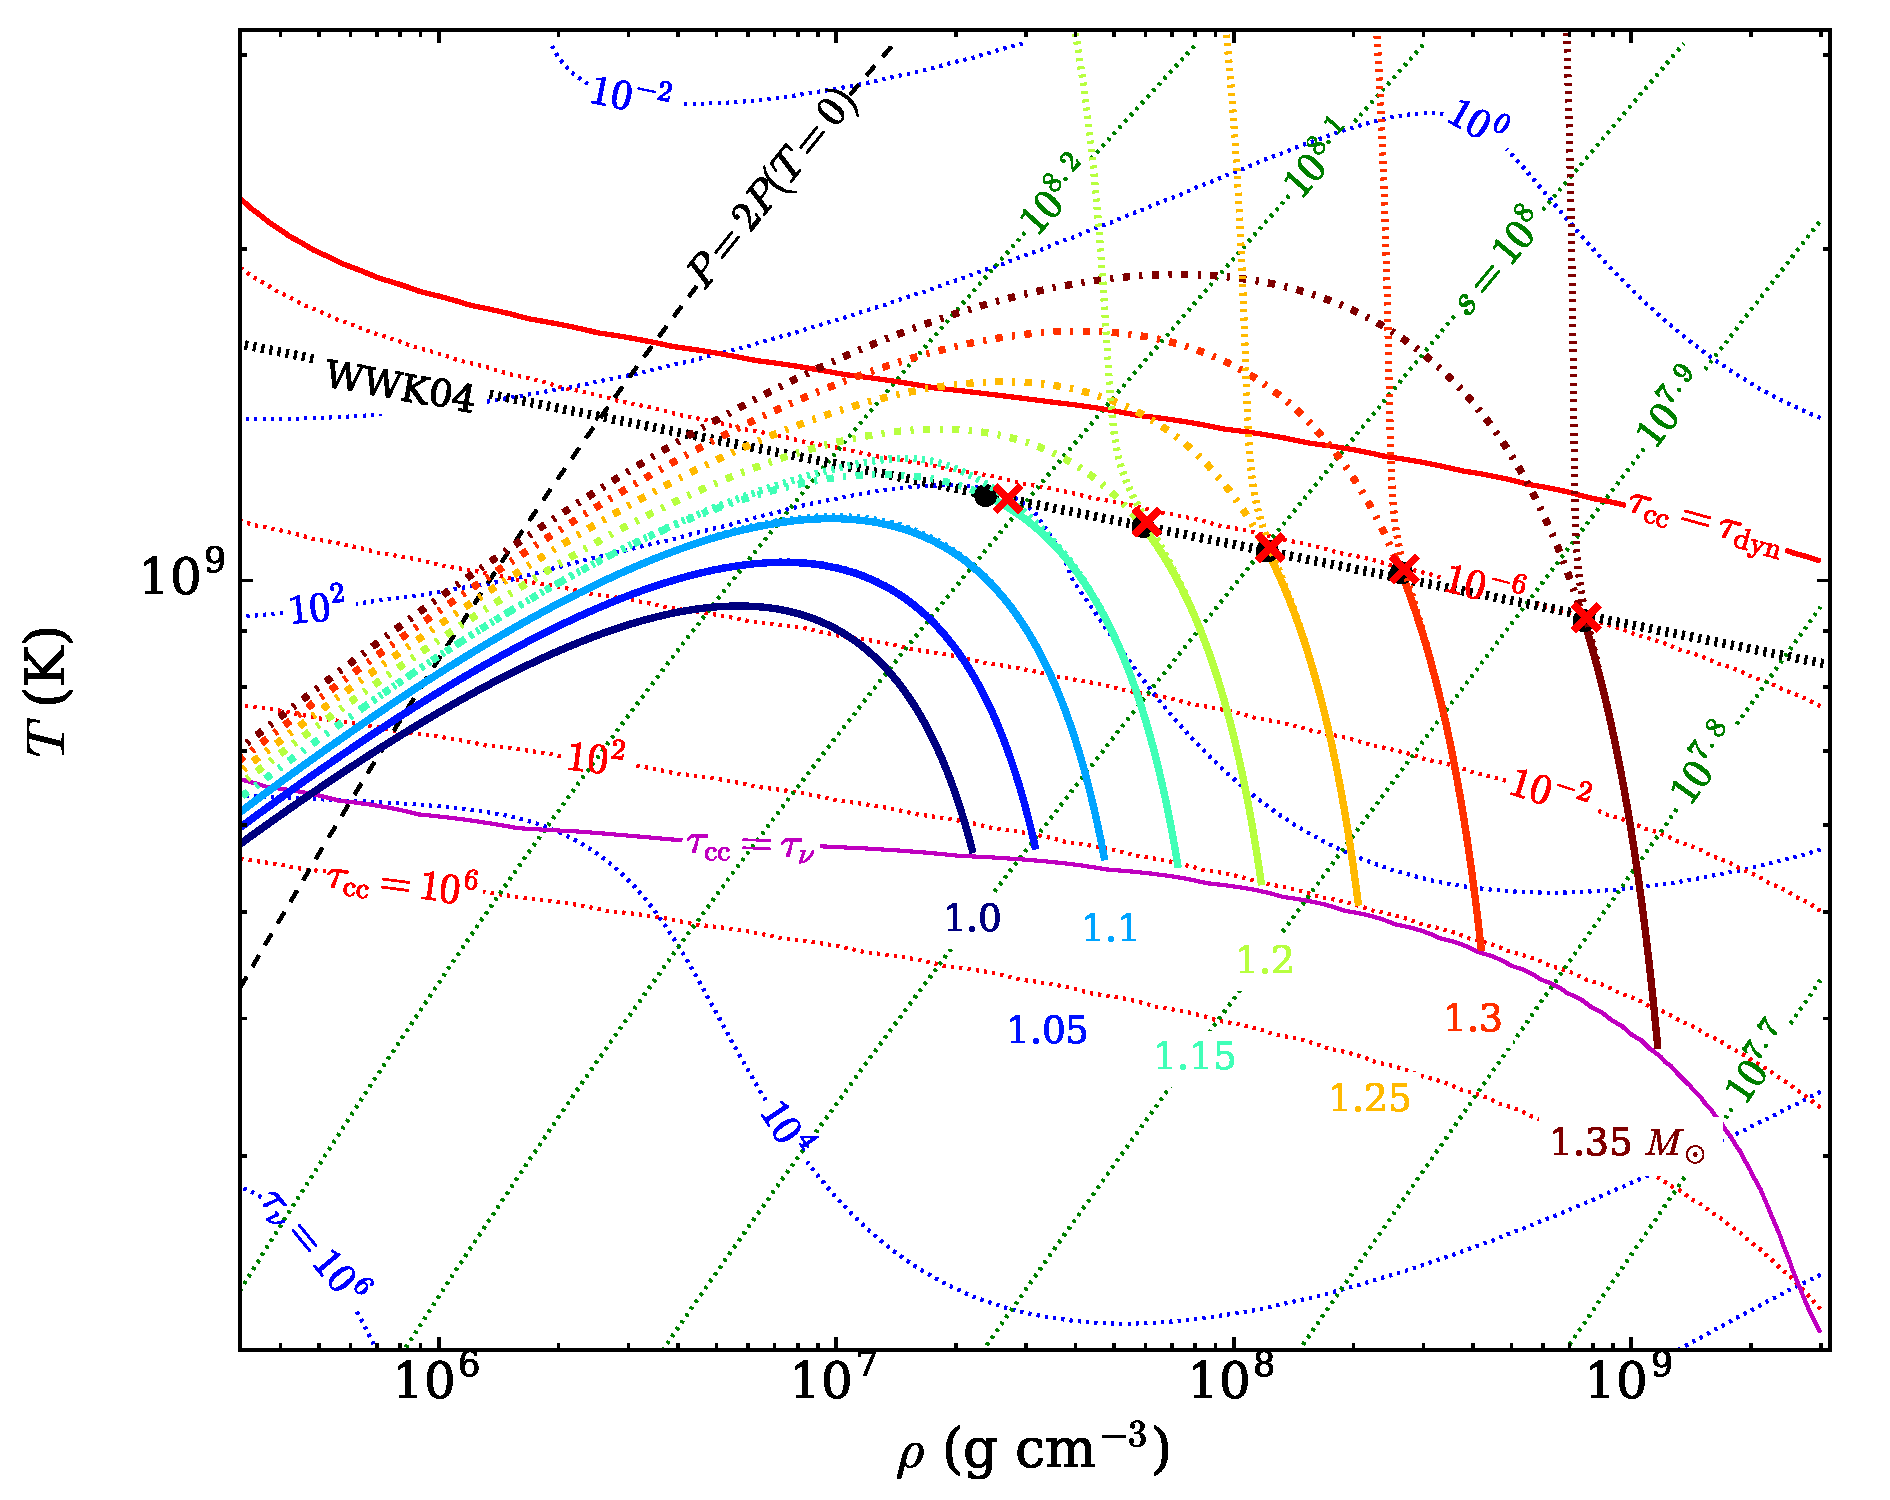
\includegraphics[angle=0,width=1.0\columnwidth]{chapter5_zhu+16/figures/runaway_rhot.pdf}
\caption{Evolution of the central temperature and density -- ``simmering tracks'' -- of simmering CO WDs with masses from $1.0 - 1.35\,\Msun$ (labeled in-line).  Solid lines represent tracks of WDs with adiabatic temperature gradients, with dash-dotted track segments indicating regions that cannot be reached during simmering.  Dotted lines represent tracks that include the superadiabatic deviation \dnabconv\ (Eqn. \ref{eq:c5_superad_dev}) required to transport the convective luminosity.  Black circles along adiabatic simmering tracks indicate ``\citeal{wooswk04} points'' where Eqn. \ref{eq:c5_endofsimmering} is first satisfied signaling the end of simmering, and the black dotted \citeal{wooswk04} line represents a power-law fit to them.  Red Xs are \citeal{wooswk04} points for \dnabconv-inclusive tracks.  Also plotted are contours of constant neutrino cooling timescale \taunu\ and carbon fusion heating timescale \taucc, both in years, as well as specific entropy $s$ in \ergpKg.  The $\taucc = \taunu$ and $\taucc = \taudyn$ lines denote where the fusion heating timescale becomes equal to the neutrino cooling timescale and dynamical timescale (Eqn. \ref{eq:c5_taudyn}), respectively.  Finally, the $P = 2P(T\mrm{=}0)$ approximates the upper bound of the region where degeneracy pressure dominates.  Timescale contours were calculated using \mesa\ \citep{paxt+11}.}
\label{fig:c5_runaway_rhot}
\end{figure}

% Values from papercalc.py/get_adiabatic_numbers()

The simmering tracks roughly form a homology parameterized by a track's highest temperature and a density-axis stretch factor.  Tracks for more massive stars reach higher temperatures and are more horizontally stretched -- the latter is due to entropy being a steeper function of density than degeneracy when $\rho\gtrsim10^8\,\gcc$ and $T\lesssim10^8\,\mrm{K}$.  The $\taucc = \taunu$ and \citeal{wooswk04} lines, though, reach lower temperatures at higher densities.  As a result, a 1.0 \Msun\ WD is already significantly less degenerate than a 1.35 \Msun\ one at the start of simmering.  By the point where the 1.0 \Msun\ WD reaches its maximum temperature of $9.5\times10^8\,\mrm{K}$ (well short of the \citeal{wooswk04} line), it has expanded considerably, its central density dropping to $\rhoc = 5.6\times10^6\,\gcc$, a quarter of its value at the onset of simmering.  It subsequently continues to expand while cooling.  A 1.35 \Msun\ WD, on the other hand, expands much less drastically -- its central density has decreased by 35\% by its \citeal{wooswk04} point at $\rhoc = 7.6\times10^8\,\gcc$, $\Tc = 9.2\times10^8\,\mrm{K}$.  This central temperature is comparable to the $\Tc = 7.8\times10^8\,\mrm{K}$ found for a \Mch\ WD by \citeal{wooswk04}, and the convective velocity we find at the top of the nuclear burning region (where $r = \Rcc$), $\vconvrcc = 8\times10^6\,\cmpsec$ ($\sim1$\% of the sound speed $c_s$) is the same value as estimated in \citeal{wooswk04} for their \Mch\ WD.  This value tends to be higher for lower-mass WDs: $\vconvrcc = 1.4\times10^7\,\cmpsec$ ($\sim3$\% of $c_s$) for a 1.15 \Msun\ WD, in agreement with our estimate of Eqn. \ref{eq:c5_vconvest2}.

The well-ordered nature of the simmering tracks extends to the \citeal{wooswk04} points, which is why they are well-represented by the \citeal{wooswk04} line.  The line falls just short of the $\taucc = \taudyn$ one, lying just underneath the $\taucc = 10^{-6}\,\mrm{yr}$ contour.  Unlike the other contours in Fig. \ref{fig:c5_runaway_rhot}, this line cannot be calculated independently of the assumptions of the runaway, though we find it is a good approximation for all of our models except for some in Sec. \ref{ssec:c5_rotmag}.

\subsubsection{Estimate of \Mcrit\ and Minimum \MNi}
\label{sssec:c5_mcritest_adiabatic}

We turn to the central task of this paper: estimating the minimum mass \Mcrit\ required to reach the \citeal{wooswk04} point, and the corresponding mass of radioactive nickel \MNi\ produced if an explosion occurs shortly thereafter.  To find \Mcrit, we generated models spaced apart by $0.005\,\Msun$, and find $\Mcrit=1.145\,\Msun$ (black simmering track in Fig. \ref{fig:c5_runaway_rhot}), which ends its simmering with $\rhoc = 2.0\times10^7\,\gcc$, $\Tc = 1.2\times10^9\,\mrm{K}$.

While an explosive event becomes inevitable once the simmering phase ends, its nature -- be it a deflagration, detonation, or some other phenomenon -- has yet to be constrained and is beyond the scope of this work.  We are, however, motivated by the resemblance of pure detonations of sub-\Mch\ WDs to SNe Ia to make a rough estimate of the mass of \Ni, \MNi, produced if the \Mcrit\ WD detonated immediately after simmering ends (i.e. without any further changes to its density structure).  Since a detonation is supersonic, and the input energy for nuclear burning is provided by the shock itself (eg. \citealt{seit+09}), nucleosynthesis in a pure detonation is, to first order, determined by the density profile of the progenitor before the explosion.  Indeed, from the results of \cite{sim+10}, we find that \MNi\ can be estimated to within a few percent by the mass of progenitor material with density $\rho>10^7\,\gcc$, $M(\rho>10^7)$ (see Fig. \ref{fig:c5_mni}).  We can use this simple relationship to estimate that for $\Mcrit = 1.145\,\Msun$, $\MNi = 0.30\,\Msun$.  

Since \Mcrit\ is the minimum mass that can reach the \citeal{wooswk04} point, 0.30 \Msun\ is the minimum amount of \Ni\ produced by any adiabatically simmering WDs (in the absence of post-simmering expansion, or the triggering of a deflagration rather than a detonation).  \MNi, however, rises quite steeply for WDs with $M>\Mcrit$: $M(\rho>10^7) = 0.39\,\Msun$ for a $1.15\,\Msun$ WD, and $0.78\,\Msun$ for a $1.2\,\Msun$ one.  This is because the density of most material in a WD is within an order of magnitude of \rhoc, and \rhoc\ at the end of simmering is a steep function of mass for tracks of $M \approx \Mcrit$, since at that point they run nearly parallel to the \citeal{wooswk04} line.  Therefore, changing \Mcrit\ by a small value, or altering the end of simmering criterion, can substantially change the minimum \MNi.

%and WDs with masses close to \Mcrit\ end simmering with $\rhoc \sim 3\times10^7\,\gcc$,We discuss this further in Sec. \ref{ssec:sensitive}.At this point, its simmering track is nearly parallel to the \citeal{wooswk04} line, suggesting a high degree of sensitivity of \Mcrit\ toward the precise criterion for the end of simmering.  We discuss this further in Sec. \ref{ssec:sensitive}.

\subsubsection{Hot Envelopes}
\label{sssec:c5_runaway_ad_hot}

%(at this temperature, thermal pressure comprises 0.003\% of the total pressure for $\rho = 10^7\,\gcc$)
%We also consider models with ``hot envelopes'' more reminiscent of merger remnants by setting $\tempiso = 2\times10^8\,\mrm{K}$ (thermal pressure is 2\% of the total at $\rho = 1\times10^7\,\gcc$) in Sec. \ref{sssec:runaway_ad_hot}, and find this has a negligible overall effect on the simmering.

%\begin{figure}
%\centering
%\includegraphics[angle=0,width=1.0\columnwidth]{adiabatic_rhot_variation.pdf}
%\caption{Comparison of adiabatic simmering tracks from Fig. \ref{fig:runaway_rhot} (solid lines) with adiabatic ones that have a hot envelope of $\tempiso = 2\times10^8$ K (dashed tracks), and ones that include superadiabatic deviation \dnabconv\ (Eqn. \ref{eq:superad_dev}; dotted lines).  Orange squares represent the \citeal{wooswk04} points for the $\tempiso = 2\times10^8$ K tracks, and cyan inverted triangles represent those for \dnabconv-inclusive ones.  All other lines and symbols are as in Fig. \ref{fig:runaway_rhot}, including the \citeal{wooswk04} line.}
%\label{fig:variations_rhot}
%\end{figure}

% Values from papercalc.py/get_hot_adiabatic_comp() and make_hot_vs_cold_critical()

Fig. \ref{fig:c2_deltamcomp} suggests mergers of WDs with similar mass lead to remnants that are heated throughout, with temperatures between $\sim 1 - 3\times10^8\,\mrm{K}$.  To roughly gauge what effect this pre-runaway heating might have, we generate models identical to the ones above, but set $\tempiso = 2\times10^8\,\mrm{K}$.  We find the simmering tracks of these ``hot-envelope'' WDs deviate most widely from their cold counterparts at the start of simmering, where their central densities are lower by $\sim3-7$\%; these differences reduce to $\sim1 - 5$\% at the end of simmering.  By then, almost the entire interior structure of an adiabatic WD, with \Tc\ $\gtrsim10^9\,\mrm{K}$, has $T > 2\times10^8\,\mrm{K}$, making its central properties insensitive to an increase in \tempiso.  Raising \tempiso\ even further may affect simmering track values more substantially, but hydrostatic solutions of WDs with $\tempiso \gtrsim 5\times10^8\,\mrm{K}$ tend to have low-density atmospheres that extend to arbitrary radii, producing objects of infinite mass.  Any WDs that were heated to such high temperatures by prior evolution, such as the remnant of \cite{ji+13} post-viscous evolution, have more complicated temperature structures that, for simplicity, will not be considered in this work.  Instead, they are explored in a companion paper (Heringer et al. in preparation).

%The $\sim5$\% ceiling comes from the 1.15 \Msun\ and 1.2 \Msun\ simmering tracks, whose simmering tracks run nearly parallel to the \citeal{wooswk04} line at the end of simmering; the actual shift in \rhoc\ for a 1.15 \Msun\ WD with $\Tc = 1.3\times10^9\,\mrm{K}$ when switching to a hot envelope is $\sim 3$\%.  

\subsection{Superadiabatic Deviation \dnabconv}
\label{ssec:c5_runaway_superad}

To more accurately calculate simmering tracks, we must include the superadiabatic temperature deviation \dnabconv\ (Eqn. \ref{eq:c5_superad_dev}) needed to carry the convective luminosity.  These \dnabconv-inclusive tracks are plotted in Fig. \ref{fig:c5_runaway_rhot} as dotted lines (without indicating track segments unreachable during simmering).  They are, regardless of mass, nearly identical to their adiabatic counterparts during simmering: their \rhoc\ and \Tc\ at the start of simmering match to within floating point precision, and, for WDs of $M > 1.2\Msun$, they also differ by less than 2\% at the end.  While the \dnabconv\ tracks do steepen and arc away from their adiabatic counterparts, this occurs only above their \citeal{wooswk04} points, which are represented by red Xs in Fig. \ref{fig:c5_runaway_rhot} and are well-approximated by the \textit{adiabatic} \citeal{wooswk04} line.  Close to \Mcrit, where the simmering tracks run nearly parallel to the \citeal{wooswk04} line, \dnabconv\ is more influential: the density of the 1.15 \Msun\ WD \dnabconv\ track at its \citeal{wooswk04} point is $\sim15$\% higher than the adiabatic value.  A mass parameter space search finds $\Mcrit=1.135\,\Msun$, which ends its simmering phase with $\rhoc = 1.7\times10^7\,\gcc$, $\Tc = 1.2\times10^9\,\mrm{K}$.  While these values are very close to the ones obtained in Sec. \ref{sssec:c5_mcritest_adiabatic}, $\MNi = M(\rho>10^7) = 0.20\,\Msun$, which is substantially lower, reflecting its sensitivity to the end of simmering criterion.

%$M(\rho>10^7)$ again rises steeply for WDs with $M>\Mcrit$: $M(\rho>10^7) = 0.45\,\Msun$ for a $1.15\,\Msun$ WD.

The overall tiny effect of \dnabconv\ is due to Eqn. \ref{eq:c5_superad_dev}'s dependence on the square of the ratio of convective velocity to sound speed, $\vconv^2/(g H_P) \approx \vconv^2/c_s^2$.  Like in the adiabatic case, near the end of simmering $(\vconvrcc/c_s(\Rcc))^2 \approx 1\times10^{-3}$ ($\vconvrcc = 1.3\times10^7\,\cmpsec$) for a $1.15\,\Msun$ star, and $1\times10^{-4}$ for a $1.35\,\Msun$ one.  This small number is partly offset by the $1/\delta = -d\ln T/d\ln \rho$ term, which approaches infinity for zero-temperature degenerate material.  Near the $\taucc = \taunu$ line, however, the entropy is already sufficiently high that $1/\delta \sim 30$ for a $1.15\,\Msun$ WD, and $\sim 300$ for a $1.35\,\Msun$ one; these values fall to $\sim 10$ and $\sim 100$, respectively, near the \citeal{wooswk04} line.  Consequently, $\dnabconv \sim 10^{-2}$, an order of magnitude smaller than $\nablaad \approx 0.3 - 0.4$.  Once the \citeal{wooswk04} point is reached, the influence of \dnabconv\ grows to beyond unity at only slightly higher \Sc\ due to the steep dependence of $\vconv^2$ on temperature, resulting in the sharp upward turn in all simmering tracks beyond that of $1.2\,\Msun$ mentioned previously.

\subsection{Rotation and Magnetic Fields}
\label{ssec:c5_rotmag}

%as well as coupling between rotation, magnetic fields and convection,

We now turn to the inclusion of rotation and magnetic fields, which are expected features of merger remnants.  These, in general, introduce complex multi-dimensional and non-local effects that are challenging to model.  To obtain rough estimates, we consider only uniform rotation or magnetic fields that vary slowly over a convective scale height, ignoring their coupling with each other and with convection, and focus on how either affect \Mcrit.  We first obtain a sense of this effect by estimating the superadiabatic temperature deviation \deltanab\ through energy balance arguments.

In the rotating case, the superadiabatic deviation \dnabrot\ can be estimated by equating the buoyancy and Coriolis forces:

\eqbegin
2\rho\Omega\vconv = -g \left(\frac{d(\Delta \rho)}{dr}\right)\Delta r = g H_P \rho \left(\frac{\delta}{H_P}\dnabrot\right)
\label{eq:c5_dnabrot_est_work}
\eqend

\noindent where $\Delta \rho$ is the density difference between a convective blob and its surroundings and we set the characteristic length of convection $\Delta r$ to $H_P$.  This gives

\eqbegin
\dnabrot = \frac{1}{\delta}\frac{2\Omega H_P}{c_s}\frac{\vconv}{c_s},
\label{eq:c5_dnabrot_est}
\eqend

\noindent where we again use $g H_P \approx c_s^2$.  Eqn. \ref{eq:c5_dnabrot_est} resembles Eqn. \ref{eq:c5_superad_dev}, with one power of $\vconv/c_s$ swapped for $2\Omega H_P/c_s \approx (\Omega^2 H_P/g)^{1/2}$, which is at most $\sim1$ for rotation at break-up.  Calculations of remnant viscous evolution \citep{shen+12, schw+12, ji+13} suggest the remnant spins down to well below critical rotation, however, and so $(\Omega^2 H_P/g)^{1/2}$ is more realistically $\lesssim10^{-1}$.  Then, for a $1.15\,\Msun$ WD near the end of simmering, $\dnabrot \lesssim (10^{-1}/\delta)(\vconv/c_s) \sim 10^{-1.5}$, an order of magnitude smaller than \nablaad; thus rotational convective suppression is a minor effect.  

In the (non-rotating) magnetized case, we can make a similar estimate by equating the buoyancy and Lorentz forces:

\eqbegin
\frac{B^2}{4\pi H_P} = -g \left(\frac{d(\Delta \rho)}{dr}\right)\Delta r = \rho g \delta \dnabmag,
\label{eq:c5_dnabmag_est_work}
\eqend

\noindent where we use the assumption that the magnetic field varies slowly over $H_P$.  This gives

\eqbegin
\dnabmag = \frac{1}{\delta}\frac{B^2}{4\pi P},
\label{eq:c5_dnabmag_est}
\eqend

\noindent where $\rho g = P/H_P$ (Eqns. \ref{eq:c5_scaleheight} and \ref{eq:c5_hydroeq}).  Calculations of magnetic field amplification in mergers (Ch. \ref{ch:ch4}) or during viscous evolution \citep{ji+13} suggest a saturation field strength of $\sim10^{11}\,\mrm{G}$ at the center of the remnant.  Given that $P \gtrsim 10^{24}\,\mrm{dyn\,cm}^{-2}$ at the centers of $\gtrsim 1.1\,\Msun$ WDs, this gives $B^2/4\pi P \lesssim 10^{-3}$, and $\dnabmag \lesssim 10^{-3}/\delta$.  Near the $\taucc = \taunu$ line, this value can be quite large, but near the end of simmering it becomes minor (eg. $\sim10^{-2}$ for a $1.15\,\Msun$ WD).

The above suggest that for reasonable rotation rates and magnetic field strengths, their effects on the simmering phase should be small.  To confirm this, we implemented the formulation of \citeauthor{stev79} (\citeyear{stev79}; hereafter \citeal{stev79}).  \citeal{stev79} incorporates rotation and externally imposed magnetic fields (both assumed, as above, to be slowly varying over $H_P$) into Rayleigh-B\'{e}nard convection.  It predicts the convective steady state -- in particular both \deltanab\ and the modified convective velocity -- by finding the growth rates of convective modes using linear stability analysis (\citeal{stev79} Sec. 2), and then equating them to their non-linear cascade rates, picking the mode with the greatest heat flux to represent the motion as a whole.  While this is \textit{ad hoc}, in the rotation-dominated and unmagnetized limit \citeal{stev79}'s theory reproduces well the convection simulations of \cite{barkdl14} over a wide range of rotation rates.  We summarize our results below; further detail can be found in Sec. \ref{sec:c5_suppression}.

For WDs with sub-critical uniform rotation, we confirm that the effect of rotation on simmering is small.  During simmering, \vconv\ increases by orders of magnitude, while $\Omega$ decreases by half an order of magnitude as the WD expands (to conserve angular momentum).  This leads $2\Omega H_P/\vconv$ to approach unity, and \dnabrot\ to approach \dnabconv, near the end of simmering for WDs with initial angular speed $\Ominit$ at about a quarter of break up speed \Omcrit.  We also find that $\vconv \propto (\dnabrot/\dnabconv)^{-1/4}$ changes very little, justifying our use of its non-rotating value in the approximation above. For moderate values of $\Omega$, then, simmering tracks shift by only a few percent in density and temperature from their non-rotating versions in Sec. \ref{ssec:c5_runaway_superad}.  For simmering when $\Ominit \rightarrow \Omcrit$, Eqn. \ref{eq:c5_dnabrot_est} suggests \dnabrot\ becomes comparable to \nablaad, but our models show that this is overshadowed by the centrifugal pressure support term in Eqn. \ref{eq:c5_hydroeq}, and the net effect is a slight reduction of \rhoc\ and \Tc\ for a model with a given \Sc.  This effect increases $\Mcrit$ to $1.14\,\Msun$ for WDs with $\Omega/\Omcrit = 0.5$, though we caution that deviations from spherical symmetry not included in our model become significant near critical rotation.

%\citeal{stev79}'s formulation states that, when the convective kinetic energy density rivals the magnetic energy density, Eqn. \ref{eq:dnabmag_est} should be replaced with Eqn. \ref{eq:superad_dev}, and so for $B \lesssim 3\times10^{11}\,\mrm{G}$ we find \dnabmag\ eventually approaches \dnabconv.

Likewise, we find that simmering tracks for non-rotating WDs with $M\approx\Mcrit$ shift by only a few percent when including magnetic fields as high as $10^{12}\,\mrm{G}$, consistent with Eqn. \ref{eq:c5_dnabmag_est}.  When performing a parameter-space search for \Mcrit, we alter field strength with mass by keeping the ratio \EBEtot\ fixed.  For $\EBEtot = 2.9\times10^{-5}$, which corresponds to $B(r=0) = 1\times10^{11}\,\mrm{G}$ in a $1.15\,\Msun$ WD at the start of simmering, $\Mcrit = 1.13\,\Msun$.  If we consider field strengths much larger than what is expected for merger remnants, however, we find that, while the simmering track still changes negligibly, the convective velocity \vconv\ becomes proportional to $1/B$ and is dramatically reduced, affecting when Eqn. \ref{eq:c5_endofsimmering} is first satisfied.  A $1.15\,\Msun$ WD threaded by a $10^{12}\,\mrm{G}$ field sees its convective velocity reduced by a factor $\sim 10 - 100$, and reaches the \citeal{wooswk04} point at $T = 8\times10^8\,\mrm{K}$, far lower than the (adiabatic) \citeal{wooswk04} line in Fig. \ref{fig:c5_runaway_rhot}.  We determine \Mcrit\ for WDs with $\EBEtot = 2.8\times10^{-3}$, which corresponds to $B(r=0) = 1\times10^{12}\,\mrm{G}$ in a $1.15\,\Msun$ WD at the start of simmering, to be $1.02\,\Msun$, a reduction of more than $0.1\,\Msun$ from the non-magnetized value.

At this strong-field limit, however, the \citeal{wooswk04} point is also well-short of the $\taucc = \taudyn$ line, meaning that a WD that reaches the point must continue to heat up before it can explode.  This heating may eventually lead to an extremely steep temperature gradient that allows for rapid convective energy transport before dynamical burning is reached, but this is beyond the ability for our model to follow.  Moreover, we strongly caution that \citeal{stev79}'s magnetic formulation may not accurately reflect non-linear magnetoconvection, except perhaps in the case of weak fields, and does not include magnetic dynamo processes, which are likely to be efficient in simmering WDs.  We discuss these further in Sec. \ref{ssec:c5_magaccuracy}.

%In the absence of rotation or magnetic fields, \citeal{stev79}'s formulation reproduces Eqns. \ref{eq:vconv_mlt} and \ref{eq:superad_dev}, except with different prefactors, i.e.

%\eqbegin
%\Fconv = 1.66\frac{\rho c_PT}{\gacc\delta} \vconv^3,  %\frac{4\pi}{75}\left(\frac{5}{2}\right)^{5/2}
%\label{eq:vconv_stev_hp}
%\eqend

%\eqbegin
%\dnabconv = 4.57\frac{\vconv^2}{\gacc\delta}\frac{1}{H_P}.
%\label{eq:superad_dev_stev_hp}
%\eqend

%\noindent We tested the effects of using this modified MLT, and find the \dnabconv\ tracks do steepen and arc away from their adiabatic counterparts,

\section{Discussion}
\label{sec:c5_discussion}

\subsection{Comparison to Observed \Mtot-\MNi\ Relations}
\label{ssec:c5_comparetoobs}

\begin{figure}
\centering
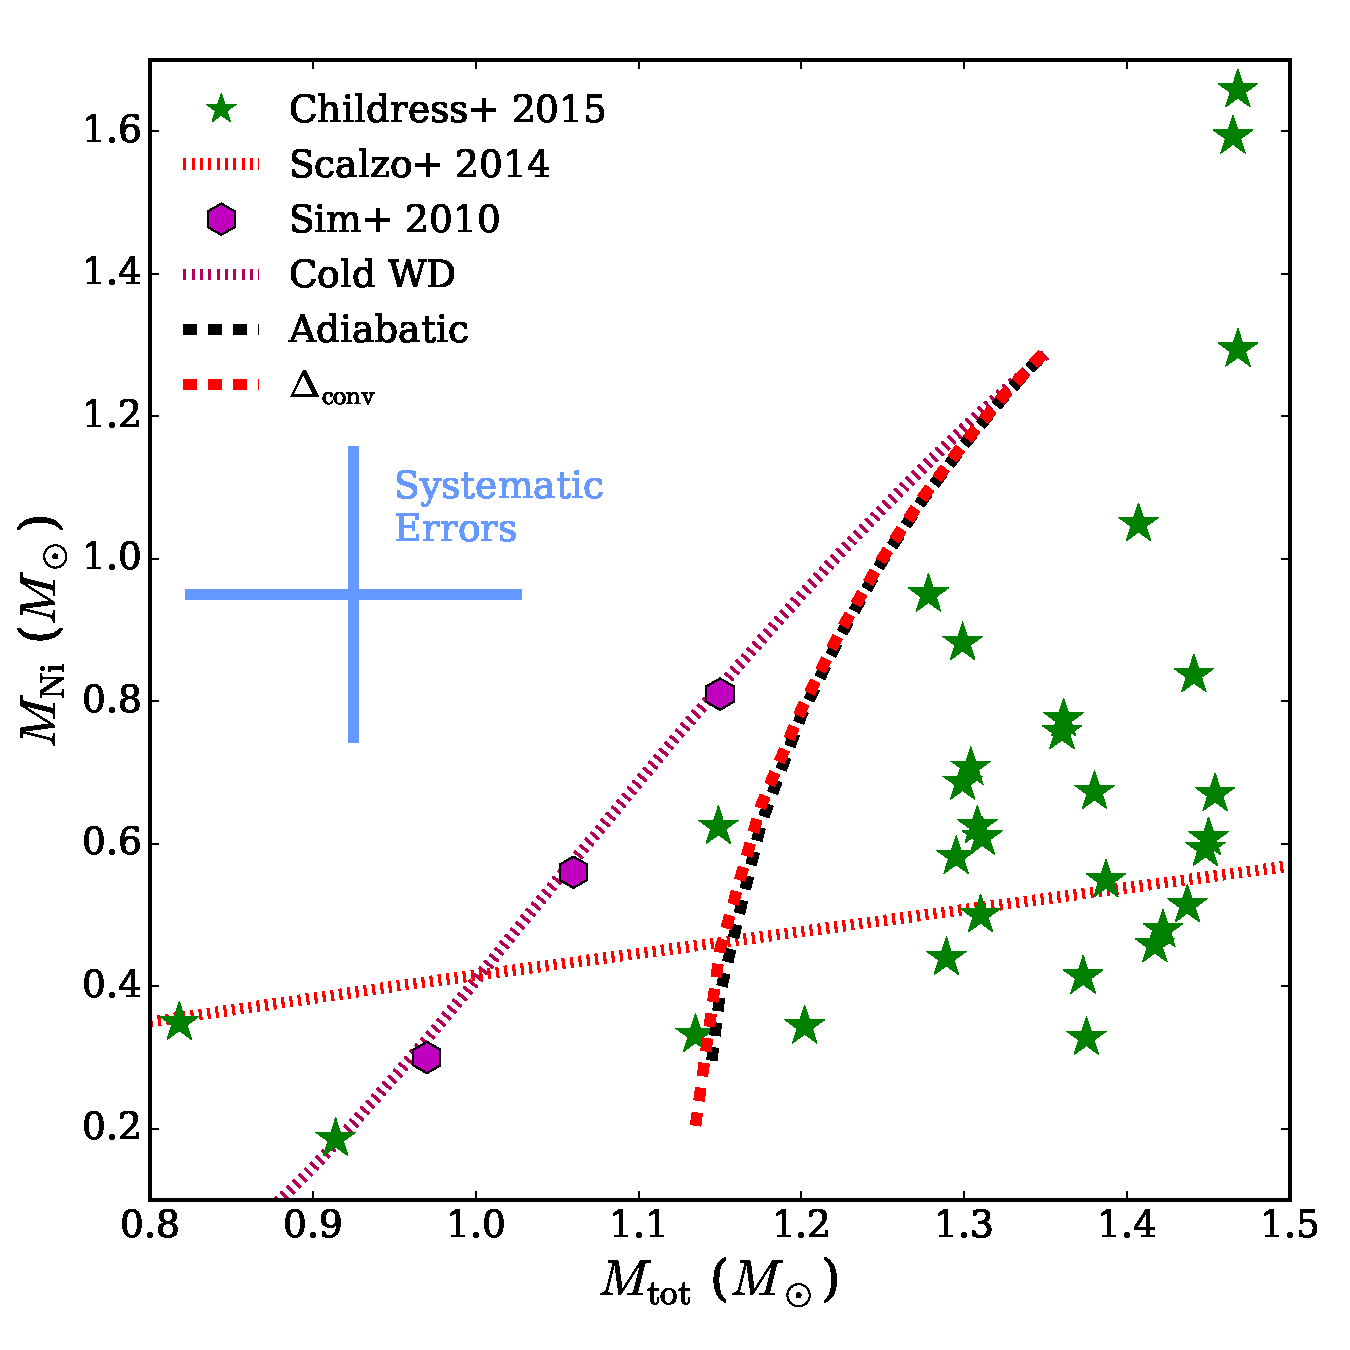
\includegraphics[angle=0,width=0.8\columnwidth]{chapter5_zhu+16/figures/mni.pdf}
\caption{Relationships between total ejected mass \Mtot\ and synthesized \Ni\ mass \MNi\ for adiabatic and \dnabconv-inclusive WDs that experience a pure detonation immediately after the end of simmering, estimated using \cite{sim+10}.  Also plotted are the \Mtot\ and \MNi\ yields of $31$ observed SNe Ia from \cite{chil+15}, and the relationship derived by \cite{scalzrs14} from 337 observed SNe Ia.  \cite{chil+15}'s systematic error bars, indicating how much their values can be shifted in unison, are also included.  The dashed magenta line is the relationship for the pure detonation of cold (uniform $10^5$ K) WDs, with the simulation results of \cite{sim+10} overdrawn.}
\label{fig:c5_mni}
\end{figure}

%Colors indicate adiabatic approximation, inclusion of \dnabconv, low ($\EBEtot = 2.9\times10^{-5}$) or high ($\EBEtot = 2.8\times10^{-3}$ magnetic field, or solid-body rotation.

We have estimated the range of masses of centrally-simmering sub-\Mch\ WDs that explode, as well as their corresponding \MNi\ yields assuming a pure detonation immediately after simmering.  Putting aside the possibility that extremely strong magnetic fields could affect \vconv, we have also determined that this range does not significantly change when including \dnabconv, rotation or magnetic fields.  It is then interesting to consider in the abstract whether these could reproduce a substantial portion of the SN Ia parameter space, and, to that end, we compare our results to estimates of ejected mass and \Ni\ yields for observed SNe Ia.  In Fig. \ref{fig:c5_mni}, we plot the $\MNi-\Mtot$ relationship for adiabatic and \dnabconv-inclusive WDs, as well as the relationship (also derived using $M(\rho>10^7)$) from the pure detonation of uniform $10^5$ K cold WD for comparison.  Additionally, results from the pure detonation simulations of \cite{sim+10} are plotted to show the accuracy of the $M(\rho>10^7)$ estimate.  Alongside these, we plot the best-fit relationship to the ejected and synthesized \Ni\ masses of $337$ observed ``normal'' \citep{bran+06} SNe Ia from \cite{scalzrs14}, and the estimated \Mtot\ and \MNi\ of $31$ normal SNe Ia from \cite{chil+15}.  \cite{scalzrs14} derives their $\MNi-\Mtot$ relationship from the observed bolometric light curve (using a range of simulated explosion models as priors; \citealt{scalz+14}), and \cite{chil+15} use \cite{scalzrs14}'s method of estimating \Mtot\ while obtaining \MNi\ from the evolution of the $[\textsc{Co\,III}]$ $\lambda5893$ emission complex during the SN Ia nebular phase.

%peak luminosity and decline rate
%, WDs with weaker ($\EBEtot = 2.9\times10^{-5}$) or stronger ($\EBEtot = 2.8\times10^{-3}$ magnetic fields and 50\% critically rotating

As expected from previous analysis, the $\MNi-\Mtot$ relationship changes little between the adiabatic and \dnabconv-inclusive WDs, being separated by a $\Mtot\lesssim0.01\,\Msun$ for any given \MNi.  While not plotted, we also found that this is true for WDs rotating at $50$\% of critical, and those with $\sim10^{11}\,\mrm{G}$ magnetic fields.  The previously-noted steep dependence of \MNi\ on \Mtot\ near \Mcrit\ is clear as well: a linear fit around $\Mtot = 1.15\,\Msun$ gives $d\MNi/d\Mtot \approx 10$ (for both curves), making it difficult to accurately estimate a minimum \MNi.  This also leads to a fine-tuning problem: to produce \MNi\ between $\sim0.3-0.6\,\Msun$ -- typical \MNi\ yields in \cite{scalzrs14} and \cite{chil+15} -- requires \Mtot\ to lie in a narrow range between $\sim 1.13 - 1.17\,\Msun$.  It is not obvious why a progenitor channel would favour this mass range, though we note the distribution of field CO WD masses is very narrowly peaked (at $0.65\,\Msun$; eg. \citealt{tremb09, klei+13}), possibly indicating that merging CO WD binaries masses fall within a narrow range.

%The simple estimate in \citeal{zhu+13}, for example, the combined mass of material in the degeneracy supported core and and thermally supported hot atmosphere -- the ``core-envelope mass'' -- is broadly distributed from $\sim 0.7 - 1.2\,\Msun$ ($\sim70 - 80$\% the mass of the accreting WD) across the mass parameter space of merging CO WDs.  

%ven if we relax the relationship to the space bounded by the Cold WD and simmering WD lines.

Nevertheless, the $\MNi-\Mtot$ relationship from pure detonations of centrally simmering CO WDs does not resemble the observed ones.  \cite{chil+15}'s values could be systematically offset by $\sim 0.1\,\Msun$ in \Mtot\ and $\sim 0.2\,\Msun$ in \MNi, but these apply to the points as a whole, and we also do not reproduce the shape of \cite{chil+15}'s distribution.  This issue is not unique to our work - \cite{scalzrs14} and \cite{chil+15} plot theoretical $\MNi-\Mtot$ curves for a wide range of proposed SN Ia progenitor classes, ranging from sub-\Mch\ WDs undergoing a double-detonation (equivalent to the Cold WD line in Fig. \ref{fig:c5_mni}) to \Mch\ pure deflagrations, and find no individual class able to reproduce the entire observed $\MNi-\Mtot$ parameter space.  If their results indeed reflect the true \Mtot-\Ni\ relationship of SNe Ia, either multiple progenitor channels are necessary, or a novel understanding of progenitors must arise.

% , an existing channel is improperly understood, or a new channel that is able to span the space must be proposed.

\subsection{Implications for Mergers as SN Ia Progenitors}
\label{ssec:c5_implications}

Regardless of whether simmering sub-\Mch\ WDs can reproduce observations, what implications do our results have on double-degenerate CO WD mergers as SN Ia progenitors, in particular the channel of \citeal{vkercj10} involving sub-\Mch\ merger remnants that ignite central nuclear fusion following their viscous evolution?  A direct mapping of post-viscous remnants onto our hydrostatic simmering WDs is not possible since their structures are quite complex, and in general their temperature profiles are substantially shallower than the convective ones used in our models.  Moreover, much of their mass exists as a hot, tenuous envelope that surrounds and exerts little pressure support on their dense, degeneracy-supported ``cores''.  As a rough estimate, we can consider the evolution of these cores as separate from their envelopes (the transition region between the two might resemble the hot atmospheres in Sec. \ref{sssec:c5_runaway_ad_hot}, and thus not affect the core's evolution).

Regardless of their initial conditions, the simmering tracks of a remnant core cannot simultaneously increase in temperature and density, since this would require part of their structure to cool (Sec. \ref{ssec:c5_numericalmodels}).  They also cannot exist, for longer than a few convective timescales, to the right of the rising portion of the simmering track of the same mass in Fig. \ref{fig:c5_runaway_rhot}, i.e. the portion of the track between the start of simmering and either the \citeal{wooswk04} point or the point of maximum temperature.  Doing so would mean its temperature gradient has become steeper than the convective one, and convective energy transport will rapidly lower the gradient back to the convective one (like for stars to the right of the Hayashi track).  As a consequence of these two restrictions, \Mcrit\ will increase for those WDs with shallow temperature profiles.  With this in mind, meaningful conclusions can be made by examining the central densities and core masses \Mc\ of post-viscous remnants.

%A direct mapping of the remnants of CO WD mergers onto hydrostatic WDs with (super)-adiabatic profiles is difficult, since these remnants will first undergo viscous redistribution of angular momentum over $10^4-10^8\,\mrm{s}$, and potentially a period of thermal evolution over $\sim10^4\,\mrm{yr}$, before igniting fusion \citep{shen+12}.  Post-viscous CO-CO remnant density and temperature profiles have been calculated for a $0.6 - 0.9\,\Msun$ remnant \citep{schw+12} and for a $0.6 - 0.6\,\Msun$ one \citep{ji+13}.  The former ignites non-degenerate carbon fusion far from the remnant center, which cannot be represented by our models, and will likely produce an oxygen-neon WD \citep{shen+12}.  The latter does ignite partly degenerate carbon fusion, but has a temperature profile that is substantially shallower than adiabatic, and so cannot simply be transliterated to a cold WD with a hot atmosphere.

To our knowledge, the sole published viscous evolution simulation of a sub-\Mch\ double CO WD merger remnant is that of \cite{ji+13}.  They find, by the end of their simulation, the central density and temperature of their $0.6 - 0.6\,\Msun$ remnant are $\sim5\times10^6\,\gcc$ and $\sim9\times10^8\,\mrm{K}$, respectively, well above the $\taucc = \taunu$ line.  Indeed, its $\taucc \sim 1\,\mrm{yr}$, much smaller than the $\gtrsim 10^4\,\mrm{yr}$ thermal contraction timescale \citep{shen+12}, so the remnant will begin to simmer.  The mass of the remnant that is within $r = 1.5\times10^9\,\mrm{cm}$ (the approximate outer boundary of the dense core in \citealt{ji+13} Fig. 1) is $\sim1.07\,\Msun$ (Suoqing Ji and Robert Fisher private communication, 2016), $\sim0.06\,\Msun$ lower than \Mcrit.  The remnant's central density is a factor of $\sim4$ lower than that for the $\sim1.05\,\Msun$ simmering track at the same temperature and a factor of $\sim6$ lower than that for the \Mcrit\ simmering track.\footnote{The remnant in \citep{ji+13} has not lost all of its rotational support by the end of their simulation, so its central density will continue to increase early in its simmering phase.  As less than a third of its initial angular momentum remains, however, it is unlikely to increase by a factor of $\sim4$.}  The most likely fate of this system is therefore expansion and possibly stable nuclear burning.  The relatively small difference between \Mc\ and \Mcrit\ suggests a merger remnant $\sim0.1\,\Msun$ more massive might possess a core mass in excess of \Mcrit.  That core's central density, though, may still be too low for simmering to end in an explosion.

%an order of magnitude lower than the \rhoc\ of any simmering tracks considered in Sec. \ref{sec:results}.

% It is thus almost certainly going to become non-degenerate and expand at temperatures well below those for dynamical burning.

For a broader parameter space of post-viscous remnants, we turn to the simple estimate of viscous evolution outcomes made in Sec. \ref{sec:c2_postmerger}.  While it tends to overestimate compression, particularly for remnants from similar-mass mergers, when compared to \citeauthor{schw+12} (and follow-up work in \citealt{rask+14}) and \cite{ji+13}, it nevertheless gives a rough estimate of the post-viscous remnant parameter space.  Taking our estimate at face value, we find that only those remnants from mergers with primary WD masses above $\sim0.8\,\Msun$ have $\rhoc \gtrsim 3\times10^7\,\gcc$, which also suggests that only remnants with total masses above \Mch\ are likely to achieve dynamical burning following viscous spin-down.  Note that the most massive of these may have instead already exploded from extreme temperatures during their mergers (for primary WD masses $\gtrsim0.9\,\Msun$; \citealt{pakm+10,pakm+11}), or due to hydrodynamic instabilities immediately afterward (for primaries $\gtrsim1\,\Msun$; \citealt{kash+15}).

If explosion is in fact not possible following viscous evolution, then sub-\Mch\ remnants that ignite carbon fusion will experience expansion instead, and eventually possible stable nuclear burning as a carbon star.  Given their properties, they are candidate progenitors for isolated high-field magnetic WDs (eg. \citealt{garc+12}), in particular hot DQ WDs (\citealt{dunlc15,dunl15thesis} and references therein), which have hot, carbon-dominated atmospheres and appear to be massive, rapidly rotating and strongly magnetized.

%Examining similar-mass remnants -- as only these have hot cores -- in \citeal{zhu+13} Fig. 16, we find ignition is achieved only for those with primary WD masses above $\sim0.8\,\Msun$; these also have central densities $\rhoc \gtrsim 5\times10^7\,\gcc$, comparable to those found along the \Mcrit\ simmering track.  

% That last estimate comes from dr/dt = sqrt(2GM/r) -> r = (2GM)^(1/3)(3t/2)^(2/3)

%wherein we generated density and temperature profiles for post-viscous remnant cores by assuming that all the remnant's angular momentum is carried away to large distance, the corresponding material forms a tenuous hot atmosphere with zero total energy, and material not carried away retains its original entropy

%Prad/Pion \propto T^3/\rho \propto \rho in adiabatic envelopes; we're in general much colder for any given density than Shen+12, so our radiation-dominated sparse atmosphere comes from magnetic reconnection (ji+13), while Shen's comes from an adiabatic non-degenerate envelope.

%This result poses a problem for the \citeal{vkercj10} sub-\Mch\ merger channel.  \cite{shen+12} finds further compression could occur during the subsequent \textit{thermal} evolution of the remnant over $\gtrsim10^4\,\mrm{yr}$, which may allow more remnants to reach higher central density and enclose more mass within their cores.  Whether central burning could still begin is uncertain, however, since thermal diffusion and neutrino-driven cooling may favor off-center carbon ignition, or simply net cooling, even for those post-viscous remnants that are initially $\gtrsim5\times10^8\,\mrm{K}$ at their center.  Moreover, remnants, with radiation-dominated and highly magnetized carbon atmospheres, will likely drive strong outflows during their thermal evolution, further complicating predictions.  We note one advantage for delaying the explosion to during thermal evolution is the removal of the ``clutter'' of the $\gtrsim0.1\,\Msun$ hot envelope surrounding the core and extending out to $\gtrsim10^{11}\,\mrm{cm}$ \citep{shen+12}.  This imparts signatures onto the explosion not seen in ordinary SNe Ia, such as a double-peaked light curve from the shock cooling of the envelope, excess blue and UV emission prior to peak light, and a slow-decaying light curve near peak light \citep{frye+10,levasg15,pirom15}.  While \cite{shen+12}'s simulation suggests thermal evolution will do little to alter the overall structure of the envelope \citep{pirom15}, it does not account for mass loss due to winds.  These will significantly alter the size and structure of the envelope, perhaps mitigating its effects on any eventual explosion.  Meanwhile, material ejected from the remnant (both during its viscous and subsequent thermal phases) moving at the escape velocity will approach $\sim10^{17}\,\mrm{cm}$ after $\sim10^4\,\mrm{yr}$.  Interaction between this material and light from the supernova could explain \citep{shen+12, ji+13} observations of SN Ia-CSM interactions such as time-variable NaID lines (eg. \citealt{pata+07, simo+09}).

\subsection{Accuracy of Magnetized Simmering Models}
\label{ssec:c5_magaccuracy}

We found in Sec. \ref{ssec:c5_rotmag} that $\lesssim10^{11}\,\mrm{G}$ magnetic fields negligibly affect simmering, while $\gtrsim10^{12}\,\mrm{G}$ ones could dramatically affect \vconv, but there are reasons to be cautious about these results, particularly in the strong field limit.

%and flow switches from steady convection to oscillatory motions along field lines.  The time averaged heat flux from these motions is much smaller

First, \citeal{stev79} does not include convective dynamo processes that amplify the magnetic field.  The vigorous convection zone found toward the end of simmering is an ideal environment for such processes -- analagous to the highly magnetized central convection zones of A and B main sequence stars (eg. \citealt{brunbt05, feat+09, augubt16}).  Amplification saturates when $\EBEconv \sim 1$, i.e. when, 

\eqbegin
B_\mrm{eq} \sim \vconv\sqrt{8\pi\rho}.
\eqend

\noindent For WDs at the end of simmering, $B_\mrm{eq} \sim 3\times10^{11}-1\times10^{12}\,\mrm{G}$.  These values match or exceed any magnetic fields generated by the merger or viscous evolution (though having fields in place at the start of simmering may increase the saturation field strength by up to another order of magnitude; \citealt{feat+09}), rendering even the low-field calculations uncertain.  Additionally, the turbulent nature of the dynamo will generate a highly tangled magnetic field that varies significantly over short length scales, unlike the large-scale fields assumed in this work; Eqn. \ref{eq:c5_dnabmag_est_work} would then suggest a much larger \dnabmag\ \citep{chabgb07}.

Second, studies of nonlinear magnetoconvection (eg. \citealt{procw82}) indicate that in steady state, magnetic fields are concentrated into high-flux bundles where the convective flow is truncated, surrounded by regions where convection continues uninhibited.  The amount of convective suppression depends on the volume fraction the bundles occupy.  When the ratio \EBEconv\ between magnetic and convective kinetic energy densities becomes higher than unity, the bundles merge and convection is effectively suppressed.  This physical picture (which is fundamentally multi-dimensional) shares little resemblance with \citeal{stev79} (Henk Spruit private communication, 2016), and no magnetic equivalent of \cite{barkdl14}'s examination of rotating convection has been conducted to see if \citeal{stev79} at least phenomenologically captures it.

%Note that $\EBEconv \ll 1$ for WDs with fields $\lesssim10^{11}\,\mrm{G}$, so this picture agrees with \citeal{stev79} that the convective flow is largely unimpeded, but this is only relevant if convective dynamo processes were inefficient.

%That said, $\EBEconv \ll 1$ for WDs with fields $\lesssim10^{11}\,\mrm{G}$ near the end of simmering, so this picture agrees with \citeal{stev79} that the convective flow is largely unimpeded.

Our model's inability to accurately follow magnetoconvection and include dynamo processes therefore constitutes the greatest uncertainty of this work.  While we have estimated that including rotation without magnetic fields is important only because it modifies the hydrostatic balance of the WD, rotation coupled with both convection and magnetic fields may additionally lead to unexpected emergent behaviour.  The multidimensional nature of magnetoconvection may also alter the end of simmering criterion -- for example, if burning material is trapped within a flux bundle, it may locally run away and lead to dynamical burning even if convection is unhindered elsewhere in the WD.  We thus stress the need for more detailed investigation into WD magnetoconvection, potentially utilizing MHD convective simulations, in the future.

%In summary, we show that simple estimates of magnetoconvection when the field is $\lesssim10^{11}\,\mrm{G}$ will have a negligible effect on the runaway.  It is likely, however, that this field will grow considerably over the course of simmering due to convective (and likely rotational as well) dynamo processes, potentially reaching $\sim10^{12}\,\mrm{G}$, where our estimates both show more drastic changes to the convective velocity, and very likely break down.  Magnetoconvection in simmering WDs will have to be investigated with more detailed and likely simulation-based analysis.

%We can say, however, that if convective dynamo processes are inefficient in simmering WDs, then then our estimates become more believable in the case of a WD with a $\lesssim 10^{11}\,\mrm{G}$ magnetic field, , as $A \lesssim 1$ by the end of its simmering.

%A naive reading of the parameter space search e a parameter-space search for \Mcrit\ in this high-field limit yields a value $\sim0.1\,\Msun$ lower than at the low-field limit, the \citeal{wooswk04} is reached when the burning timescale is far longer than dynamical.
  

%and $\MNi = 0.21\,\Msun$

%However, we have already mentioned in Sec. \ref{ssec:magaccuracy} that these results, particularly those at the high-field limit, must be treated with caution.  \citeal{stev79}'s magnetic formulation has not yet been numerically tested and may not accurately reflect non-linear magnetoconvection, except perhaps in the case of weak fields.  Moreover, dynamo processes are likely to be efficient in simmering WDs and will likely lead to $\sim10^{12}\,\mrm{G}$ fields near the end of simmering, dominating over any fossil fields from prior evolution.


%In conclusion, we cannot constrain the magnetic field strength
%
% for two reasons.  First, studies of nonlinear magnetoconvection (eg. \citealt{procw82}) indicate that in steady state, fields are concentrated into bundles where the flow is truncated, surrounded by regions where convection continues uninhibited; convective suppression depends on the volume fraction the flux bundles occupy.  If magnetic dominates over convective energy density, the flux bundles merge and convection is effectively suppressed.  This picture bears little obvious resemblance to \citeal{stev79}'s formulation (Henk Spruit personal communication), and no equivalent to \cite{barkdl14} has been conducted to see if \citeal{stev79} is at least phenomenologically accurate.  The second and more important issue is that convective dynamo processes, neglected in our analysis, are likely to amplify any pre-existing magnetic fields by orders of magnitude during simmering.  The saturation field strength can be estimated by equating the magnetic and convective kinetic energy densities to obtain $B_\mrm{eq} \sim \vconv\sqrt{8\pi\rho}$.  For the WDs at the end of simmering, $B_\mrm{eq} \sim 3\times10^{11}-1\times10^{12}\,\mrm{G}$ (having strong fields in place at the start of simmering may increase these values by up to another order of magnitude; \citealt{feat+09}).  Coupling between convection and magnetic fields -- as well as rotation, in the most general case -- cannot be analyzed with \citeal{stev79}'s framework.  We therefore must leave investigation magnetoconvection to more detailed and likely simulation-based analysis methods.

%All this suggests that the fiducial 0.6-0.6\Msun merger proposed as a SN Ia progenitor by \cite{vkercj10} (and simulated by \cite{ji+13}) will expand and cool long before it achieves dynamical burning.  The remnants that can follow this simmering channel are likely to be similar-mass merger remnants whose total mass exceeds 1.8 Msun, which are rarer than even \Mch mergers (by definition!).

%The post-viscous evolution merger remnants of shen and ji, or the estimates from zhu+13, cannot directly be represented by spherically symmetric hydrostatic WDs.  Nevertheless, approximate translations can be made by either mapping the central density or mass which is degenerately supported into a simmering track.  the results of post-merger evolution studies like Application to Ji+13 results.  Further compression Badenes + Moaz for rare superchandra.

%-Should note in results section that having a hot atmosphere basically doesn't alter the interior.  Modifications to the temperature structure close to the centre of the remnant SHOULD do so, but only serve to lead to becoming nondegenerate earlier.

%It should first be noted that spun-down merger remnants cannot directly be mapped onto hydrostatic WDs with (super)-adiabatic profiles, since they tend to have more complex temperature profiles that are generally substantially shallower than adiabatic, and so cannot simply be represented by a cold WD with a hot atmosphere.  However, we can make rough comparisons, especially considering that in Sec. XXX, we noted that having a tenuous thermally supported atmosphere does little to alter the evolution of the simmering, degenerate core.  Post merger evolution simulations show that the final configuration of the spun-down remnant is indeed a degenerate core (cold or hot) surrounded by a tenuous atmosphere, and so we can map that cold degenerate core mass to a simmering track.  In Zhu+13, we make a rough estimate of the spun-down remnant profile, assuming that the rotational energy is dissipated entirely in the outer regions of the remnant, forming a hot atmosphere.  We find that about 75\% of the total mass of the remnant remains as a degenerate central object rather than a tenuous envelope, regardless of the mass ratio of the merging WDs.  This is supported by the simulations of Shen+12 of the PME of dissimilar mass merger remnants over a large range of total mass - they find the total mass within a cold core and a hot, isothermal plateau, to be 75\% the total mass (these all have cold cores, though, so wouldn't be represented by a center-lit runaway).  It is difficult to tell exactly what's going on in Ji's results, though an integration of the density profile within $10^9$ cm suggests a core mass of 0.8 Msun, somewhat lower than the 75\% we suggested.  If this 75\% thing holds, then only remnants of similar-mass mergers with total mass \textit{above} \Mch\ could form simmering cores above the critical mass.

%The estimate in zhu+13, and ji+13's results, also suggest the central density of the merger remnants of 0.65-0.65\Msun mergers is around 10**6.5, much lower than the \rhoc\ of the simmering \Mcrit\ WD at the same temperature.  Since \rhoc can only go down with increasing entropy, and being at lower \rhoc means being much closer to the degeneracy line, this system's evolution is highly likely to be expansion.

%We also do not consider the interplay between rotation, convection and magnetic field evolution, especially the growth of magnetic fields due to convective dynamos, and how they can be affected by the pre-existing field from the remnant.  As we found tentative evidence with our \citeal{stev79} estimate that field strengths on the order of $10^{12}\,\mrm{G}$, albeit larger than reasonable estimates for field strengths produced before or during simmering, may dramatically affect the convective velocity, this is a particularly interesting avenue of investigation.  The inherent complexity and multidimensional nature of the problem suggests that any future estimates of the temperature structure and convective velocity should be motivated by magnetohydrodynamic simulations of WD convection {\charles REFERENCES?}.  Finally, we use the analytic 1D dynamical burning criterion to determine the end of simmering, and a better estimate can be found by taking into account the range of temperatures and velocities individual convecting blobs may have (\citeal{wooswk04}) and how these can change because of, eg. magnetic fields altering the global convective flow patterns.

\section{Conclusions}
\label{ssec:c5_conclusions}

We investigated using simple estimates the outcome of simmering for sub-\Mch\ WDs, and find that the minimum mass \Mcrit\ that achieves dynamical burning and explodes, rather than expanding and cooling, is $1.135\,\Msun$.  We also estimate that including rotation or $\lesssim 10^{11}\,\mrm{G}$ magnetic fields alters this value by less than $\sim0.01\,\Msun$ and $\sim0.02\,\Msun$, respectively.  Stronger, $\sim10^{12}\,\mrm{G}$ fields, which may be generated through convective dynamo processes, could affect simmering much more substantially, but are beyond the scope of our models.  Examining merger remnants in Ch. \ref{ch:ch2}, and the simulation of \cite{ji+13}, we estimate that the majority of sub-\Mch\ post-viscous remnants are too underdense to remain degenerate until dynamical burning if simmering were to set in.  Even if they could explode, they would still produce very little \Ni.  This presents an issue for to the viability of the \citeal{vkercj10} channel, as it suggests most sub-\Mch\ remnants do not explode as SNe Ia.

% We also find that simmering is well-described by approximating the convective zone's temperature profile as adiabatic, with $\Mcrit$ changing by just $\sim0.01\,\Msun$ compared to more accurate models.  and we stress the merit of further study

Ours is a first-order estimate of the simmering process.  Aside from the clear need for more advanced prescriptions of magnetoconvection, future models would also benefit from including eg. modifications to the convective velocity structure resulting from heating or work to expand the WD as it becomes non-degenerate (\citeal{piroc08}, though their effects will primarily be felt far from center of the WD).  A more accurate analysis of the simmering of post-viscous merger remnants could be made by directly using their simulated density, temperature and rotation profiles as initial conditions.  We also use the analytic 1D criterion of \citeal{wooswk04} to determine the end of simmering, and better estimates can be made by taking into account the range of temperatures and velocities of individual convective flows.  This has already been done for \Mch\ WDs using 3D hydrodynamic simulations \citep{kuhlwg06, zing+09, zing+11, nona+12}, which could be extended to lower-mass WDs.

% Zing+09 Fig. 9, 10, gives ignition at slightly lower temperature of 7e8 K.  Zing+11 Fig. 6 gives similar value, as does Nona+12 Fig. 3

We have also estimated the \Mtot-\MNi\ relationship of simmering sub-\Mch\ WDs that reach explosion and find that they, like many other models, do not correspond to the observed SN Ia \Mtot-\MNi\ relationships of \cite{scalzrs14} and \cite{chil+15}.  In particular, our most massive WDs produce too much \Ni\ to reproduce the bottom right of Fig. \ref{fig:c5_mni}, which would not be the case if the temperature structure at the end of simmering were substantially shallower than in our models.  Such a structure could potentially be produced if the burning were not center-lit, but occurred in an off-center shell that remained degenerate throughout the runaway, and we explore this possibility in the companion paper to this work (Heringer et al. in preparation).

\vspace{5mm}

We are very grateful to Ken Shen, whose discussion with MHvK on the existence and value of \Mcrit\ years ago served as the original inspiration for this paper, and to Henk Spruit for his insights into magnetoconvection and its implementation in our models.  We also thank Chris Matzner, Yuri Levin and Chris Thompson for helpful comments, and Suoqing Ji and Robert Fisher for both valuable feedback and for sharing the end-state of their viscous evolution simulation.  Our calculations made extensive use of Frank Timmes' Helmholtz EOS and sections of \mesa\ by Bill Paxton and the \mesa\ consortium, and we them for making these codes publically available.  

%This work was partly based off of and motivated by unpublished work by Philip Chang, Heidi White and Marten H. van Kerkwijk

%Meanwhile, detonations can potentially also be triggered by the collision of two convective flows (independent of the end of simmering criterion), and 1D simulations of the onset of detonation suggest that this could occur in {\charles material with $\rho = XXX$, $T = XXX$}, well short of (Chang et al. in preparation).


\section{Appendix: Convective Suppression due to Rotation and Magnetic Fields}
\label{sec:c5_suppression}

In this appendix, we detail our calculations of rotating and magnetized simmering WDs.  In general, their inclusion greatly complicates the treatment of convection inside a star by introducing non-spherically symmetric alterations to the convective structure, non-ideal magnetohydrodynamic (MHD) effects, and coupling, generally non-local, between the magnetic field, rotation profile and convective structure.  Because the purpose of this work is to provide only rough estimates for the effects of rotation and magnetic fields, a full treatment of these is well beyond its scope.  We instead implement the simple modifications to \deltanab\ and \vconv\ derived by \citeal{stev79}.

\citeal{stev79} linearizes the Boussinesq MHD equations.  By assuming the convection is Rayleigh-B\'{e}nard (planar geometry, with uniform vertical gravitational field and background temperature gradient) and that all perturbations to fluid variables can be written as sums of modes $\propto\exp({\bf k}\cdot{\bf x} + \sigma t)$, he obtains the dispersion relation

\begin{eqnarray}
\sigma^4 + \sigma^2\left(2\frac{({\bf k}\cdot{\bf B})^2}{4\pi\rho} + \frac{(2\boldsymbol{\Omega}\cdot{\bf k})^2}{k^2} + N_*^2\frac{k_\perp^2}{k^2}\right) + \nonumber \\
\left(\frac{({\bf k}\cdot{\bf B})^2}{4\pi\rho}\right)^2 + \left(\frac{({\bf k}\cdot{\bf B})^2}{4\pi\rho}\right)N_*^2\frac{k_\perp^2}{k^2} = 0
\label{eq:c5_stev79dispersion}
\end{eqnarray}

\noindent in the limit of zero magnetic dissipation; $\sigma$ is the temporal growth rate of a given mode and $N_*^2 = -g\delta\Delta/H_P$ is the Brunt-V\"{a}is\"{a}l\"{a} (buoyancy) frequency.  \citeal{stev79} then assumes that, for modes with $\sigma > 0$, the non-linear terms in the Boussinesq equations eventually limit their growth, leading to $\sigma$ equalling the nonlinear cascade rate $\sim kv$ at the convective steady state \citep{barkdl14}.  He also assumes convection at steady state is dominated by the mode that transports the greatest heat flux.  The former assumption leads to a relationship between $\sigma$, the mode velocity $v$ (equivalent to \vconv) and wavevector ${\bf k}$:

\eqbegin
\sigma = v/k.
\label{eq:c5_stev79saturation}
\eqend

\noindent Eqns. \ref{eq:c5_stev79dispersion} and \ref{eq:c5_stev79saturation} can then be combined with the mode heat flux

\eqbegin
F = \frac{\rho c_PT}{g\delta}\frac{\sigma^2}{k^2}\left(\sigma + \frac{1}{\sigma}\frac{({\bf k}\cdot{\bf B})^2}{4\pi\rho}\right)
\label{eq:c5_stev79flux}
\eqend

\noindent to determine the one that dominates thermal transport.

For non-rotating, unmagnetized WDs, this formulation reproduces Eqns. \ref{eq:c5_vconv_mlt} and \ref{eq:c5_superad_dev} from MLT, except with prefactor coefficients:

\eqbegin
\Fconv = \frac{4\pi}{25}\left(\frac{5}{2}\right)^{5/2}\frac{\rho c_PT}{\gacc\delta l_m} \vconv^3,
\label{eq:c5_vconv_stev}
\eqend

\eqbegin
\dnabconv = \frac{25\pi^2}{6}\frac{\vconv^2}{\gacc\delta}\frac{H_P}{l_m^2}.
\label{eq:c5_superad_dev_stev}
\eqend

\noindent \citeal{stev79} point out that, for his formulation to reproduce the current age, luminosity and effective temperature of the Sun within a 1D stellar evolution model, it must be calibrated by using $l_m \approx 3H_P$.  In order to be consistent with our non-rotating and unmagnetized results from before, we shall contine to use Eqns. \ref{eq:c5_vconv_mlt} and \ref{eq:c5_superad_dev} rather than Eqns. \ref{eq:c5_vconv_stev} and \ref{eq:c5_superad_dev_stev} when considering rotation and magnetic fields below.  We consider the result of using these modified coefficients in Sec. \ref{ssec:c5_sensitive_apdx}.

%leading to Eqns. \ref{eq:vconv_stev_hp} and \ref{eq:superad_dev_stev_hp}

For WDs that are rotating or magnetized, \citeal{stev79} finds that his $\Delta$ and \vconv\ can be written as multiplicative factors of the \dnabconv\ and \vconv\ of Eqns. \ref{eq:c5_vconv_stev} and \ref{eq:c5_superad_dev_stev} (using the same \Fconv).  As such, we define \vconvzero\ and \dnabconvzero\ as the convective velocity and temperature gradient calculated assuming \textit{no} rotation or magnetic field.

To further simplify our estimates, we shall assume that the rotation is solid-body and magnetic fields vary slowly over a scale height, and we will consider rotation separately from magnetic fields.  The former is enforced by our use of \citeal{stev79}'s model, since its Rayleigh-B\'{e}nard setup assumes $\boldsymbol{\Omega}$ and ${\bf B}$ are constant over its vertical lengthscale ($H_P$).  At least for rotation, it is also a plausible representation of merger remnant cores, which tend to eliminates differential rotation during post-merger viscous evolution.  Considering rotation and magnetic fields separately allows us to independently gauge the relative importance of each to the runaway.  \citeal{stev79}'s theory also does not include coupling between rotation, convection and magnetic fields.  This neglects, in particular, magnetic field amplification by convective dynamos, which is discussed further in Sec. \ref{ssec:c5_magaccuracy}.

\subsection{Simmering of Rotating White Dwarfs}
\label{ssec:c5_runaway_rot}

The exact solution in the rotating case is given by \citeal{stev79}:

\begin{eqnarray}
\frac{\dnabrot}{\dnabconvzero} + \frac{6}{25\pi^2}\rossby^2 &=& \left(\frac{\dnabrot}{\dnabconvzero}\right)^{5/2} \nonumber \\
\frac{\vconv}{\vconvzero} &=& \left(\frac{\dnabrot}{\dnabconvzero}\right)^{-1/4}
\label{eq:c5_rot_exactsoln}
\end{eqnarray}

\noindent where Rossby number

\eqbegin
\rossby = \frac{\vconvzero}{2\Omega l_m} = \frac{\vconvzero}{2\Omega H_P}
\label{eq:c5_rossbynumber}
\eqend

\noindent is a proxy for the ratio between convective and rotational velocities in the convection zone.\footnote{Like \cite{barkdl14}, we assume ${\bf g}||\boldsymbol{\Omega}$ for our calculations; in the case where the two are misaligned, the convective suppression is reduced by a factor ${\bf g}\cdot \boldsymbol{\Omega}/g\Omega$.}  \citeal{stev79} (their Eqn. 43) provide approximations to Eqn. \ref{eq:c5_rot_exactsoln} in the limits of very large and very small \rossby\ (their Eqns. 42 - 43), and in lieu of solving for $\dnabrot/\dnabconvzero$ during integration, we use the approximation

\eqbegin
\frac{\dnabrot}{\dnabconvzero} \approx \left(1 + \left(0.23\rossby^{-4/5}\right)^2\right)^{1/2},
\label{eq:c5_rot_nabrat_apx}
\eqend

\noindent where $0.23\rossby^{-4/5}$ is the \citeal{stev79} approximation for $\dnabrot/\dnabconvzero$ for $\rossby \ll 1$:\footnote{Using a quadrature averaging of the \citeal{stev79} $\rossby \ll 1$ and $\rossby \gg 1$ expressions is impossible because they do not cross each other.}

\eqbegin
\frac{\dnabrot}{\dnabconvzero}  \approx 0.23\rossby^{-4/5}.
\label{eq:c5_rot_nabrat_apx_low}
\eqend

\noindent Eqn. \ref{eq:c5_rot_nabrat_apx} is accurate to within 3\% of the exact $\dnabrot/\dnabconvzero$ for all \rossby, and $\vconv/\vconvzero = (\dnabrot/\dnabconvzero)^{-1/4}$ to within 1\%.  Eqn. \ref{eq:c5_rot_nabrat_apx_low} can be approximated by $\dnabrot \sim \delta^{-1}(H_P\Omega/c_s)(\vconv/c_s)$, which can be compared to a na\"{i}ve implementation of the (1D analog of the) Solberg-H{\o}iland stability criterion, $\Delta_\mrm{Solberg} \sim \delta^{-1}(H_P\Omega/c_s)^2$ (eg. \citealt{tass00} Sec. 3.4.2).  The replacement of one $H_P\Omega/c_s$ term with $\vconv/c_s$ accounts for the lack of suppression along the axis of rotation, and the turbulent cascade of polar convection into modes orthogonal to the rotation axis in the nonlinear regime \citep{barkdl14}.

%In the limits of very large and very small \rossby, Eqn. \ref{eq:rot_exactsoln} can be approximated by

%\eqbegin
%\dnabconv =
%    \begin{cases}
%      \dnabconvzero(1 + 1/(62\rossby^2)), & \rossby \gg 1 \\
%      0.23\rossby^{-4/5}\dnabconvzero, & \rossby \ll 1.
%    \end{cases}
%\label{eq:rot_approxsoln_dnab}
%\eqend

%\eqbegin
%\vconv =
%    \begin{cases}
%      \vconvzero(1 - 1/(242\rossby^2), & \rossby \gg 1 \\
%      1.5\rossby^{1/5}\vconvzero, & \rossby \ll 1.
%    \end{cases}
%\label{eq:rot_approxsoln_dnab}
%\eqend

Notably, this formulation has been tested in the $\rossby \ll 1$ limit by \cite{barkdl14}, who show through simulations of rotating Rayleigh-B\'{e}nard convection that $\dnabrot \propto \Omega^{4/5}$ and $\vconv \propto \Omega^{-1/5}$ over $10^{-4} \lesssim \rossby \lesssim 10^{-1}$, consistent with \citeal{stev79}.  While not a simulation of a convecting star, this lends credence to \citeal{stev79}'s assumptions for convective transport and nonlinear mode saturation.

% of the first model above the $\taucc = \taunu$ ignition line

Conservation of angular momentum and solid-body rotation are both assumed for the entirety of the runaway, constraining $\Omega$ such that it only needs to be specified for one model along the simmering track; naturally, we choose the one at the start of simmering.  This is done by specifying the model's \Sc\ to be that for the start of simmering in the (non-rotating) adiabatic track of the same mass WD.  Since we show below that rotation does not substantially affect the runaway, this is a reasonable approximation for the start of simmering \Sc\ in the rotating case.  We then set the WD angular speed at this point, \Ominit, to some fraction of its critical value \Omcrit.  To determine \Omcrit, profiles are generated with increasing angular speed until a pressure inversion ($dP/dm > 0$) is detected during integration.  By Eqn. \ref{eq:c5_hydroeq}, this means that the layer $dm$ is spinning at near-Keplerian speeds; the corresponding angular speed \Omcrit\ is then analagous to the solid-body break-up angular speed (though not equal to it, since Eqn. \ref{eq:c5_hydroeq} assumes spherical symmetry).  Note that this procedure is only done to set $\Omega$ to a reasonable fraction of the break-up angular speed near the start of simmering, and does not otherwise affect our runaway calculations.

\begin{figure}
\centering
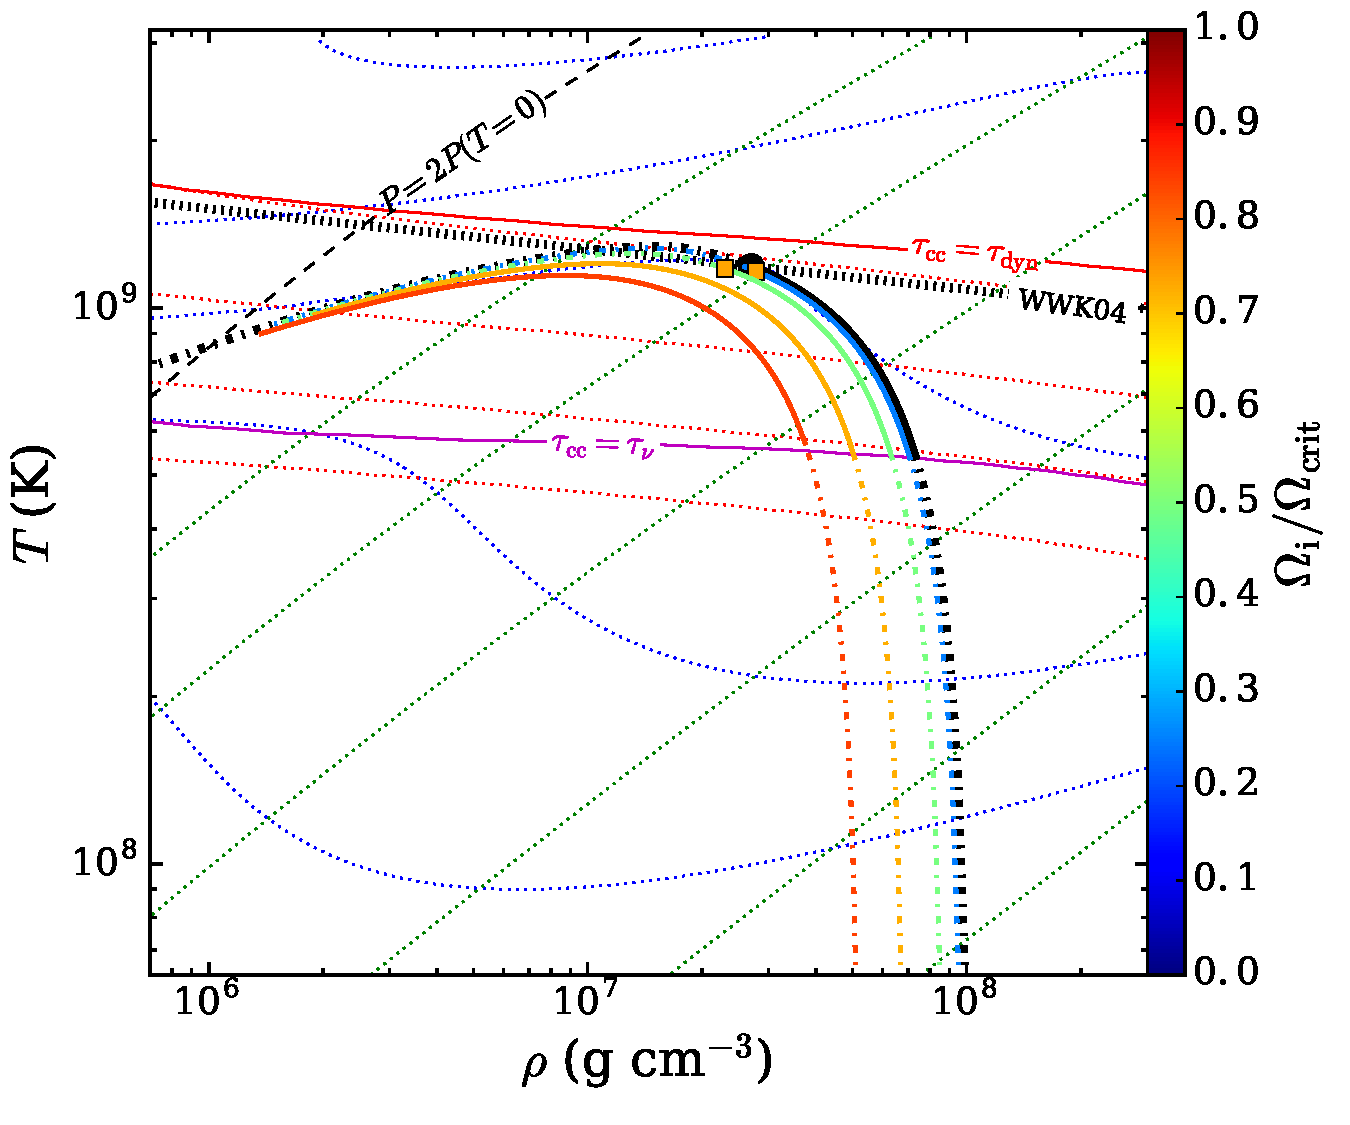
\includegraphics[angle=0,width=0.8\columnwidth]{chapter5_zhu+16/figures/rot_stev_1pt15_rhot.pdf}
\caption{Simmering tracks for (unmagnetized) solid-body rotating $1.15\,\Msun$ WDs.  Track color represents $\Ominit/\Omcrit$, the ratio of the WD's angular speed at the start of simmering to its numerically determined break-up value, and the thicker black track is the non-rotating \dnabconv-inclusive $1.15\,\Msun$ one from Fig. \ref{fig:c5_runaway_rhot}.  \citeal{wooswk04} points are a black circle for the non-rotating track and orange squares for the rotating ones; the curves with $\Ominit/\Omcrit > 0.75$ never satisfy Eqn. \ref{eq:c5_endofsimmering}.  Dash-dotted track segments indicate solutions that cannot be reached during simmering.  All other lines and symbols are as in Fig. \ref{fig:c5_runaway_rhot}.}
\label{fig:c5_rot_stev_1pt15_rhot}
\end{figure}

%\eqbegin
%\deltanab_\mrm{GTSH} = \deltanab_\mrm{GT} + \deltanab_\mrm{SH}.
%\eqend

In Fig. \ref{fig:c5_rot_stev_1pt15_rhot}, we plot the simmering tracks of $1.15\,\Msun$ WDs with $\Ominit/\Omcrit$ varying from 25\% - 85\% of $\Omcrit = 0.61\,\mrm{s}^{-1}$ ($1.15\,\Msun$ is chosen for its proximity to the adiabatic \Mcrit\ value).  Below $10^{8}\,\mrm{K}$, the rotating WD tracks shift leftward (in density) from the non-rotating one (thick black line) -- from a factor of $0.03$ for $\Ominit/\Omcrit = 0.25$ to a factor of $1.9$ for $\Ominit/\Omcrit = 0.85$ -- due to centrifugal support supplementing degeneracy pressure.  This partial lifting of degeneracy competes with the convective suppression effects of rotation.  \citeal{stev79} notes the suppressive effect can be estimated by combining Eqns. \ref{eq:c5_superad_dev} and \ref{eq:c5_rot_nabrat_apx_low}:

\eqbegin
\dnabrot \approx 0.23\rossby^{-4/5}\dnabconvzero \sim \left(\frac{\Omega H_P}{\vconvzero}\right)^{4/5}\frac{\vconvzero^2}{g H_P} = \dnabconvzero^{3/5}\left(\frac{\Omega^2 H_P}{g}\right)^{2/5}.
\label{eq:c5_rot_limitapprox}
\eqend

\noindent All stars have $\Omega^2 H_P \lesssim g$, and so at best $\dnabrot \sim \dnabconvzero^{3/5}$.  For a $1.15\,\Msun$ WD rotating at less than a third of the critical rate, $\dnabconvzero \sim 10^{-2}$ near the end of simmering (Sec. \ref{ssec:c5_runaway_superad}) and $\dnabrot \lesssim 10^{-1.5}$, a $\lesssim10$\% deviation to \nablaad.  Our calculations give even more modest values: $\dnabrot/\nablaad \sim 0.03$ ($\dnabrot/\dnabconvzero \sim 1$) near the \citeal{wooswk04} point of both the $\Ominit/\Omcrit = 0.25$ and $\Ominit/\Omcrit = 0.50$ tracks.  These are lower than what Eqn. \ref{eq:c5_rot_limitapprox} predicts because for small values of $\Ominit$, $\rossby \sim 1$ near the end of simmering and Eqn. \ref{eq:c5_rot_nabrat_apx} approaches its non-rotating counterpart.  At the start of simmering, $\rossby \ll 1$ and $\dnabrot/\dnabconvzero \sim 200$ for the $\Ominit/\Omcrit = 0.50$ track, but $\dnabconvzero \sim 10^{-7}$ at this point, and so it makes little difference to the overall runaway.  Near critical rotation, Eqn. \ref{eq:c5_rot_limitapprox} predicts $\dnabrot \sim 10^{-1}$ which is more comparable to \nablaad, but our calculations show centrifugal support has a much larger effect on the runaway by lowering both \rhoc\ and \Tc\ of a model with a given \Sc.  This, in fact, reduces the effect of convective suppression by lowering \vconv.  Thus, rotation primarily serves to lift degeneracy and prevent a WD from reaching its \citeal{wooswk04} point.  At a modest $\Ominit/\Omcrit = 0.25$, the WD reaches its \citeal{wooswk04} point with $\rhoc = 2.8\times10^7\,\gcc$, only $\sim3$\% higher than its non-rotating counterpart.  As rotation increases, \rhoc\ at the \citeal{wooswk04} point decreases: it is $15$\% lower for the $\Ominit/\Omcrit = 0.50$ track, and tracks with higher rotation rates fail to reach the \citeal{wooswk04} point entirely.

The convective velocity, meanwhile, has a very shallow dependency on $\dnabrot/\dnabconvzero$.  At the end of simmering, $\vconvrcc = 1.1\times10^7\,\cmpsec$ for both the $\Ominit/\Omcrit = 0.25$ and $\Ominit/\Omcrit = 0.50$ tracks, comparable to the non-rotating value of $\vconvrcc = 1.3\times10^7\,\cmpsec$ (Sec. \ref{ssec:c5_runaway_superad}).  The $\sim20$\% difference in \vconvrcc\ is due to the sensitivity of \epscc\ and the \citeal{wooswk04} criterion to changes in temperature. 

%-- near the end of simmering small changes in temperature lead to large changes in \vconvrcc.

From the above analysis, it is unsurprising that a mass parameter space sweep for simmering WDs with $\Ominit/\Omcrit = 0.50$ yields $\Mcrit = 1.14\,\Msun$.  

%The corresponding $\MNi = 0.31\,\Msun$, though this is again much less well-constrained due to how much \rhoc\ changes near the simmering track turnover.  

Our results near critical rotation should be taken with a grain of salt, since deviations from spherical symmetry not reproducible by our model become significant. However, a merger remnant is unlikely to be critically rotating at the start of simmering.  As mentioned previously, studies of post-merger viscous evolution all find the remnant core spins down to well below critical rotation \citep{shen+12,schw+12,ji+13}.  While these works do not constrain the amount of vestigial rotation, we have shown above that modest rotation rates in general do little to influence the runaway.

\subsection{Simmering of Magnetized White Dwarfs}
\label{ssec:c5_runaway_mhd}

Like in the rotating case, the exact solution for the (dissipationless) magnetic case has no simple analytical form.  \citeal{stev79} finds in the limit of large Alfv\'{e}n ratio

\eqbegin
A = \frac{v_A^2}{\vconvzero^2} = \frac{B^2}{4\pi\rho\vconvzero^2}
\label{eq:c5_alfven_ratio}
\eqend

\noindent that \dnabmag\ and \vconv\ can be approximated as\footnote{We assume the magnetic field is aligned with the gravitational vector, and hence $\cos^2\phi = 1$ in Sec. 4 of \citeal{stev79}.  We have also corrected a coefficient error in \citeal{stev79}'s $\vconv/\vconvzero$ expression.}

%\noindent derived using an energy variation principle.  \Bv is the magnetic field in the radial direction and, as \cite{mullm01} notes, $\Bv(r)$ is a spherical mean-square averaging of the true field geometry.  In this work we only specify this spherically symmetric profile, and so drop the subscript with the understanding that the true 3D geometry may have significant $\hat{\theta}$ and $\hat{\phi}$ components.  For merger remnants, \cite{ji+13} and \cite{zhu+15}'s simulations both find the poloidal and toroidal field components in rough equipartition, suggesting \Bv\ is within a factor of $\sim2$ of field strength $B$.  $\gamma$ is the effective polytropic exponent, which we take to be \gammaad\ (the ratio of specific heats).  $1/\gamma_\mathrm{ad} = \alpha - \delta \nablaad$ and $\p\ln\rho/\p\ln P = \alpha - \delta\nabla$; combining these with Eqn. \ref{eq:gt66crit} gives  

%NOTES:
% - estimate of dynamo potential using R_m (Chabrier 2007 pg 2 paragraph 2)

\begin{eqnarray}
\frac{\dnabmag}{\dnabconvzero} &=& 0.24A \nonumber \\
\frac{\vconv}{\vconvzero} &=& 1.21A^{-1/2}
\label{eq:c5_mag_exactsoln}
\end{eqnarray}

\noindent Again, in lieu of solving for $\dnabmag/\dnabconvzero$ exactly during integration, we use the approximations 

\begin{eqnarray}
\frac{\dnabmag}{\dnabconvzero} &\approx& \left(1 + \left(0.24A\right)^{6/5}\right)^{5/6}, \nonumber \\
\frac{\vconv}{\vconvzero} &\approx& \left(1 + \left(1.21A^{-1/2}\right)^{-13/4}\right)^{-4/13}.
\label{eq:c5_mag_apx}
\end{eqnarray}

\noindent Exponents $6/5$ and $-13/4$ were obtained by empirically minimizing these functional forms to the numerically calculated exact solutions over a range $10^{-4} < A < 10^4$.  $\dnabmag/\dnabconvzero$ in Eqn. \ref{eq:c5_mag_apx} is accurate to within $2$\% of its exact solution, and $\vconv/\vconvzero$ to within $3$\%.  We assume the magnetic field is frozen to its corresponding mass shell $m$ throughout the runaway, changing in strength to satisfy conservation of flux $d\Phi \propto B r^2$ (i.e. $B(m) \propto 1/r(m)^2$), meaning that, analagous to the rotation case above, the magnetic field only needs to be specified for one model in the runaway.  We again take the \Sc\ of this model to be that for the start of simmering in the equivalent adiabatic simmering track.  We set the initial field profile $B_0(m)$ to be one where

\eqbegin
\dmag = \frac{B_0^2}{8\pi P}
\label{eq:c5_cdev}
\eqend

% papercalc_arepo.py plots the spherical field profile of the 0.625 - 0.65 Msun remnant at 200, 600 and 1000 s after coalescence - we see that the B vs. m profile vaguely in broad strokes looks similar to a \dmag profile for a hydrostatic WD, but the \dmag vs. m profile increases with radius, peaking at ~0.7M_tot and then decreasing sharply.  We shouldn't take these comparisons too seriously, since we cannot compare a non-rotating equilibrated WD with a rotating one recently birthed from a merger.

\noindent is held constant, suggested by \cite{macdm09}, who use it to study magnetic convective suppression in brown dwarfs, as a reasonable profile for a star whose density does not vary wildly over most of its interior.  The spherically averaged magnetic field profile of the merger remnant in Ch. \ref{ch:ch4} also resembles Eqn. \ref{eq:c5_cdev} near the center of its core, though caution must be used comparing a recently formed merger remnant with a hydrostatic simmering WD.  The central initial field strength \Binit\ is restricted to below $10^{12}\,\mrm{G}$ to keep $\dmag \ll 1$ ($\dmag = 0.01$ when $\Binit = 2.0\times10^{12}\,\mrm{G}$ for a $1.15\,\Msun$ WD at the ignition line).  This allows us to leave out magnetic terms in Eqn. \ref{eq:c5_hydroeq}.

%As we know of no reasonable scenario to form a WD where $\Pmag/\Pgas \sim 0.1 - 1$, even in a process as violent as a merger \citep{vkercj10,wicktf14,ji+13, zhu+15}, this is unlikely to be a prohibitive restriction.

\begin{figure}
\centering
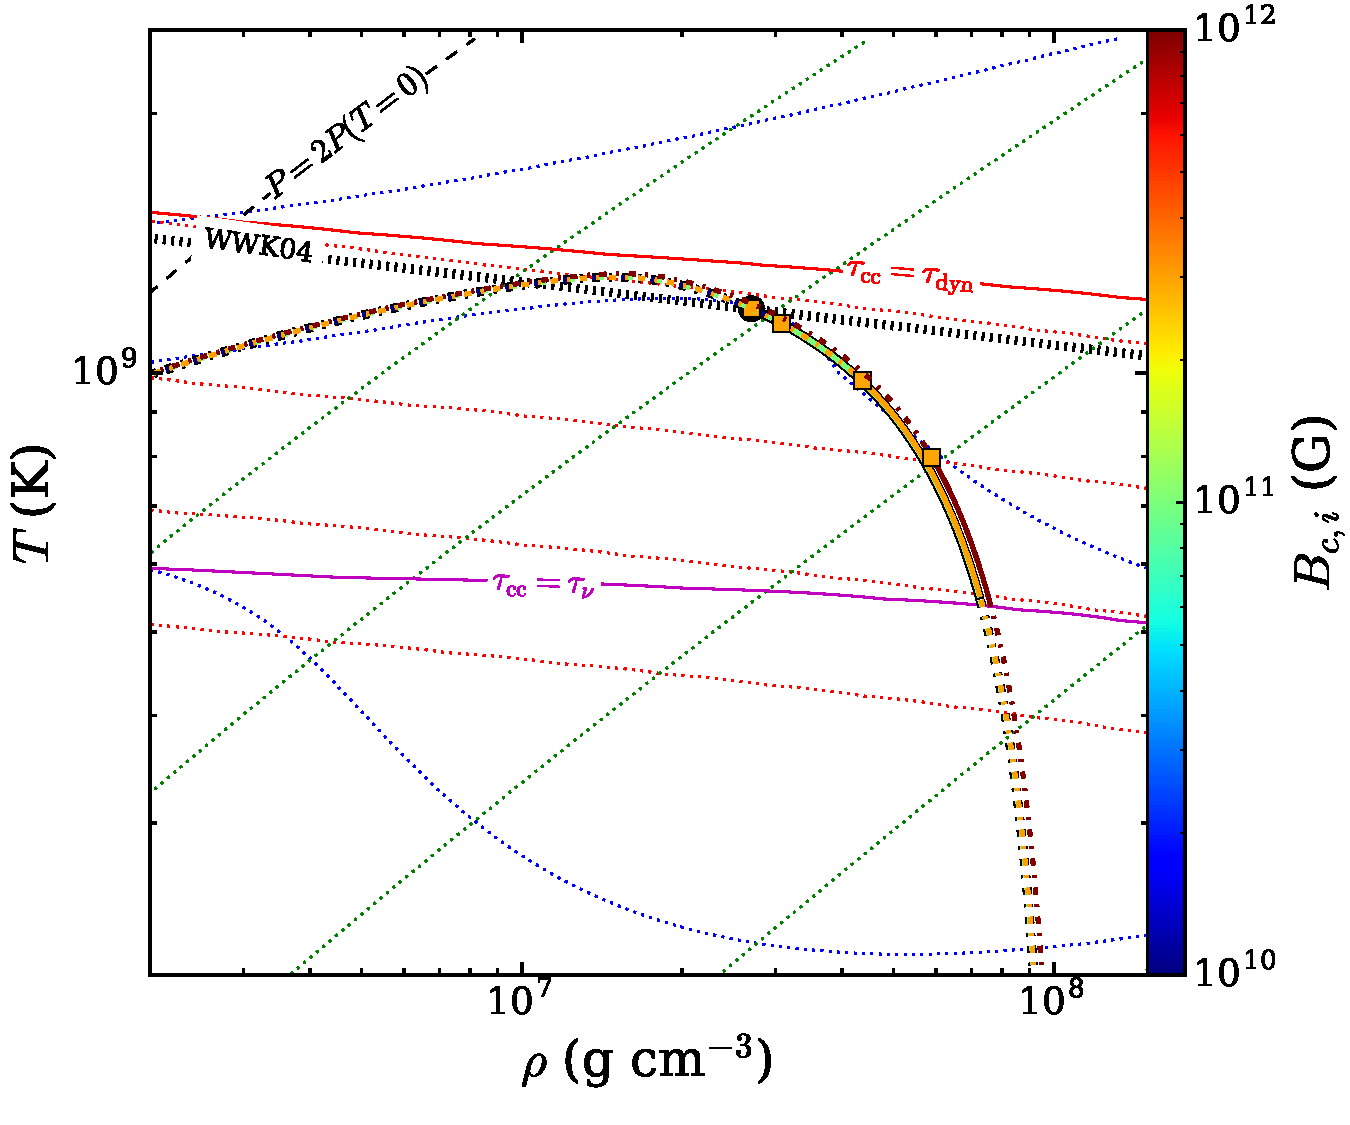
\includegraphics[angle=0,width=0.8\columnwidth]{chapter5_zhu+16/figures/mag_1pt15_rhot.pdf}
\caption{Simmering tracks for (non-rotating) magnetized $1.15\,\Msun$ WDs.  Track color represents the central magnetic field strength at the start of simmering, \Binit, and the thicker black dotted track is the non-magnetized \dnabconv-inclusive $1.15\,\Msun$ one from Fig. \ref{fig:c5_runaway_rhot}.  All other lines and symbols are as in Fig. \ref{fig:c5_rot_stev_1pt15_rhot}, except that the orange circles represent \citeal{wooswk04} points for the magnetized (rather than rotating) tracks.}
\label{fig:c5_mag_1pt15_rhot}
\end{figure}

Fig. \ref{fig:c5_mag_1pt15_rhot} depicts simmering tracks for a $1.15\,\Msun$ with $\Binit = 1\times10^{10}-1\times10^{12}\,\mrm{G}$.  Across the entire range of field strengths, the shift in the simmering track shape due to \dnabmag\ is small.  The \rhoc\ values of the magnetized tracks deviate by $\lesssim5$\% from the non-magnetized one, even for the strongest field strengths being considered.  This is because, for $A \gg 1$, Eqn. \ref{eq:c5_mag_exactsoln} can be rewritten as

\eqbegin
\dnabmag \approx \frac{1}{\delta}\frac{B^2}{16\pi \rho g H_P} = \frac{1}{\delta}\frac{B^2}{16\pi P},
\label{eq:c5_mag_apx_high}
\eqend

\noindent or $\dmag/2\delta$.  Note that Eqn. \ref{eq:c5_mag_apx_high} is identical to Eqn. \ref{eq:c5_dnabmag_est}, obtained by balancing the buoyancy and Lorentz forces, and a similar expression is derived in \cite{macdm09} based on one from \cite{gougt66}.  Since we consider fields with $\dmag < 3\times10^{-3}$, \dnabmag\ is large only when $1/\delta$ is.  This is the case close to the $\taucc = \taunu$ line, leading to $\dnabmag/\nablaad \sim 0.2$ for the $\Binit = 10^{12}\,\mrm{G}$ track, but for colder and highly degenerate WDs their temperature profile has little influence on their density profile.  When $T\gtrsim10^9\,\mrm{K}$, $1/\delta$ is much smaller and \dnabmag\ approaches \dnabconv\ in value.

\vconv, however, is proportional to $A^{-1/2}$ when $A \gg 1$, and can be many orders of magnitude smaller than \vconvzero\ during the earlier phases of simmering.  For the $\Binit = 1\times10^{12}\,\mrm{G}$ track, \vconv\ is reduced so much that Eqn. \ref{eq:c5_endofsimmering} is satisfied at $\rhoc = 5.9\times10^7\,\gcc$, $\Tc = 8.0\times10^8\,\mrm{K}$, well-below the adiabatic \citeal{wooswk04} line.  At the \citeal{wooswk04} point for the $\Binit = 1\times10^{12}\,\mrm{G}$ run, $A \sim 3\times10^3$, and hence $\vconvrcc = 1.3\times10^{4}\,\cmpsec$, a factor of $\sim30$ smaller than \vconvzero\ and $\sim10^3$ smaller than \vconvrcc\ at the end of simmering for the unmagnetized track.  This reduction appears only for $\Binit \gtrsim 3\times10^{11}\,\mrm{G}$; for the $\Binit = 1\times10^{11}\,\mrm{G}$ one, simmering ends when $A \sim 10^{-1}$, and \rhoc\ and \Tc\ deviate from from their non-rotating values by $14$\% and $4$\%, respectively.

%at $\rhoc = 3.1\times10^7\,\gcc$, $\Tc = 1.1\times10^9\,\mrm{K}$

We perform a parameter space search of WDs with either low or high-strength magnetic fields.  Strength is defined as the magnetic to total energy ratio \EBEtot; ``low'' means $\EBEtot = 2.9\times10^{-5}$ and ``high'' means $\EBEtot = 2.8\times10^{-3}$, equivalent to $\Binit = 1\times10^{11}\,\mrm{G}$ and $\Binit = 1\times10^{12}\,\mrm{G}$, respectively, for a $1.15\,\Msun$ WD at the start of simmering.  Similar to the non-rotating case, the low field search yields $\Mcrit = 1.13\,\Msun$.  The high field search yields $\Mcrit = 1.02\,\Msun$, a reduction of more than $0.1\,\Msun$ from the non-magnetized case.  The latter estimates are the most uncertain out of all those in this work, which is discussed at length in the main paper.  

%and $\MNi = 0.21\,\Msun$

%\MNi\ grows from $\MNi = 0.26$ for $1.05\,\Msun$ to $\MNi = 0.75\,\Msun$ for $1.15\,\Msun$.  The latter value is around twice \MNi\ of the unmagnetized $1.15\,\Msun$ simmering track because the \citeal{wooswk04} point occurs so much earlier in the magnetized case, before the WD has the chance to expand significantly from its zero-temperature density structure.

%and \MNi\ rapidly grows to $0.51\,\Msun$ for a $1.15\,\Msun$ WD

However, we have already mentioned in Sec. \ref{ssec:c5_magaccuracy} that these results, particularly those at the high-field limit, must be treated with caution.  \citeal{stev79}'s magnetic formulation has not yet been numerically tested and may not accurately reflect non-linear magnetoconvection, except perhaps in the case of weak fields.  Moreover, dynamo processes are likely to be efficient in simmering WDs and will likely lead to $\sim10^{12}\,\mrm{G}$ fields near the end of simmering, dominating over any fossil fields from prior evolution.

%Our \Mcrit\ and \MNi\ values are instead estimates of the maximum possible effect, equivalent to assuming the simmering track becomes vertical once reaching the \citeal{wooswk04} point.  While our results then show that extremely strong magnetic fields can potentially reduce \Mcrit\ by more than $0.1\,\Msun$, $10^{12}$ G is more than an order of magnitude higher than the peak field strength produced during or after a merger \citep{ji+13,zhu+15}.  A $10^{11}\,\mrm{G}$ field is likely to be more realistic, and results in a much less extreme deviation from the non-rotating case.

%We have thus shown that the simmering track for a WD with reasonable rotation rates or magnetic field strengths deviates by $\lesssim10$\% for all values, except \MNi, from its non-rotating and unmagnetized counterpart.  The non-rotating, unmagnetized runaway itself is well-approximated by an adiabatic simmering track.

%A field of $1\times10^{12}\,\mrm{G}$ is also $\sim30$ times greater than the average strength within the core of the remnant reported in the simulations of \cite{ji+13} and \cite{zhu+15}.\footnote{The total magnetic energies reported from both simulations are also a factor of $\gtrsim20$ smaller those of the $1\times10^{12}\,\mrm{G}$ tracks, but this is much harder to compare due to the density and magnetic field structures in the  simulations extending far from the remnant core.}  The value of $B^2/(B^2 + 4\pi\gamma P)$ must remain low for more realistic magnetic field strengths, making any changes to the runaway process likely to be minor.  Indeed, \Binit\ must remain $\lesssim3\times10^{11}\,\mrm{G}$ for a uniform field and $\lesssim2\times10^{12}\,\mrm{G}$ for a constant \dmag\ field to keep the ratio of magnetic to degeneracy pressure $P_\mrm{mag}/P_\mrm{deg} \lesssim 10^{-2}$ throughout the WD.

\subsection{Sensitivity to Mixing Length Theory Coefficients}
\label{ssec:c5_sensitive_apdx}

We noted above that that \citeal{stev79}'s formulation reproduced the equations of MLT in the non-rotating, unmagnetized limit, except for differing prefactor coefficients, and that to reproduce the properties of the Sun it had to further be calibrated by setting $l_m \sim 3$.  Both $l_m$ and the coefficients vary among different formulations of convection.  To get a sense of the robustness of our estimate for \Mcrit\ and \MNi\ to these variations, we generate a simmering track for a $1.15\,\Msun$ WD where we replace the ``default'' Eqns. \ref{eq:c5_vconv_mlt} and \ref{eq:c5_superad_dev} with Eqns. \ref{eq:c5_vconv_stev} and \ref{eq:c5_superad_dev_stev}, respectively, and set $l_m = 3$.  This is practically equivalent to rescaling \vconv\ by a factor of $0.85$, and \dnabconv\ by a factor of $3.26$.

%\eqbegin
%\Fconv = \frac{4\pi}{25}\left(\frac{5}{2}\right)^{5/2}\frac{\rho c_PT}{\gacc\delta l_m} \vconv^3,
%\label{eq:vconv_stevcal}
%\eqend

%\eqbegin
%\dnabconv = \frac{25\pi^2}{6}\frac{\vconv^2}{\gacc\delta}\frac{H_P}{l_m^2}.
%\label{eq:superad_dev_stevcal}
%\eqend

%\noindent in lieu of Eqns. \ref{eq:vconv_mlt} and \ref{eq:superad_dev}.

\begin{figure}
\centering
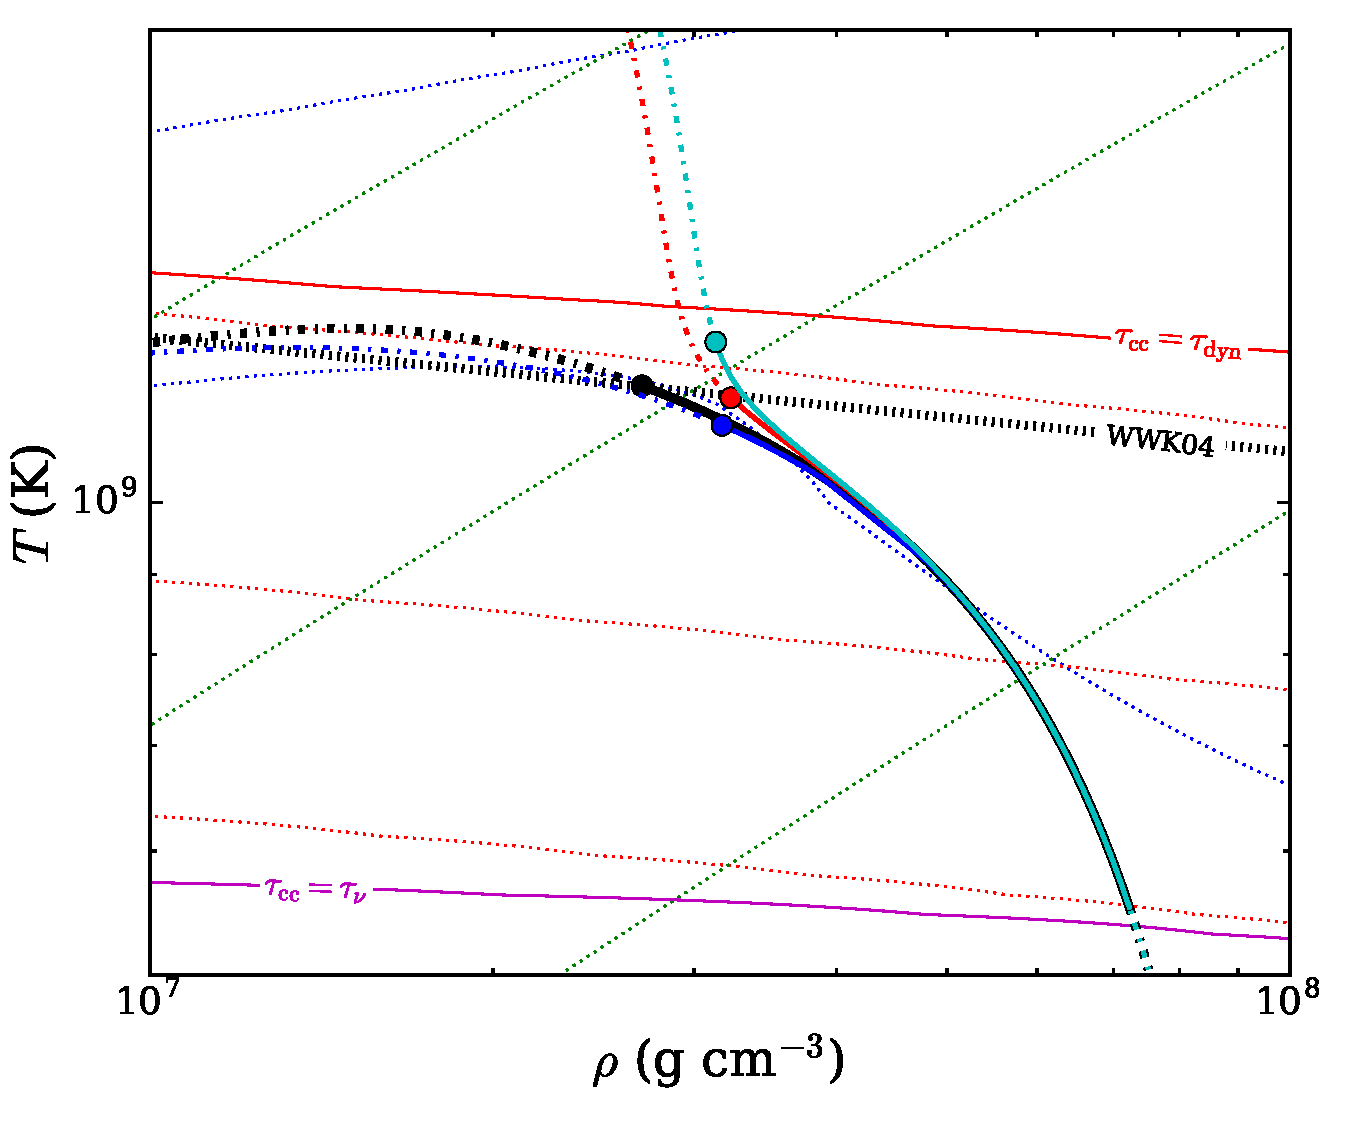
\includegraphics[angle=0,width=0.8\columnwidth]{chapter5_zhu+16/figures/diag_1pt15_rhot.pdf}
\caption{Comparison of a simmering track for a non-rotating, unmagnetized $1.15\,\Msun$ WDs calculated using Eqns. \ref{eq:c5_vconv_stev} and \ref{eq:c5_superad_dev_stev} (red line) with the ``default'' $1.15\,\Msun$ one that uses Eqns. \ref{eq:c5_vconv_mlt} and \ref{eq:c5_superad_dev} from Fig. \ref{fig:c5_runaway_rhot} (black).  Also plotted are tracks which use Eqn. \ref{eq:c5_superad_dev} but multiply a prefactor of $2$ (blue) or $1/2$ (cyan) to Eqn. \ref{eq:c5_vconv_mlt}.  Circles along each track indicate their respective \citeal{wooswk04} points.  All other lines and symbols are as in Fig. \ref{fig:c5_rot_stev_1pt15_rhot}.}
\label{fig:c5_mltcoeff_rhot}
\end{figure}

In Fig. \ref{fig:c5_mltcoeff_rhot}, we compare the \citeal{stev79} coefficient (SC; solid red line) track with the one using default coefficients (solid black).  There is little difference between the two lines until close to the end of simmering, where increased superadiabaticity leads to a steepening of the SC track; it ends simmering with $20$\% higher \rhoc.  Adding $50$\% critical rotation or a $10^{11}$ G magnetic field yields additional deviations of $\sim10$\% in \rhoc\ near the end of simmering.  A mass parameter-space search of \Mcrit\ for the SC tracks yields $\Mcrit = 1.12\,\Msun$, a deviation on par with those seen in previous sections.

%($\MNi = 0.2\,\Msun$)

The \citeal{stev79} coefficients only modify \vconv\ by $15$\%, so the deviations above are due to the change in \deltanab.  Since Eqn. \ref{eq:c5_superad_dev} also depends on \vconv, modifying it can result in comparable changes.  In Fig. \ref{fig:c5_mltcoeff_rhot} we show tracks calculated using Eqn. \ref{eq:c5_superad_dev} as is, but multiplying a factor of $2$ (``$2v$''; blue dashed) or $1/2$ (``$v/2$''; cyan dashed) to Eqn. \ref{eq:c5_vconv_mlt}.  The larger \deltanab\ in the $2v$ track leads it to steepen near the end of simmering like the SC one, while the $v/2$ track more resembles the adiabatic one in Fig. \ref{fig:c5_runaway_rhot}.  Altering \vconv\ also changes where Eqn. \ref{eq:c5_endofsimmering} is satisfied.  The $v/2$ track reaches its \citeal{wooswk04} point when $\vconvrcc = 4.4\times10^6\,\cmpsec$ and with $18$\% higher \rhoc\ ($6$\% lower \Tc), than the default track; the $2v$ track ends simmering when $\vconvrcc = 4.3\times10^7\,\cmpsec$, but also with $16$\% higher \rhoc\ ($7$\% higher \Tc) due to it being steeper.  A search of \Mcrit\ for $v/2$ and $2v$ tracks both give $\Mcrit = 1.12\,\Msun$.

%(($\MNi = 0.15\,\Msun$) for $v/2$, $\MNi = 0.2\,\Msun$ for $2v$).

%The combined effects a modified prescription and near-critical rotation or a much stronger magnetic field are more substantive (since the effects of the latter two are also multiplicative): while, for example, while the default coefficient $10^{12}$ G simmering track in Fig. \ref{fig:mag_1pt15_rho} closely follows its non-magnetized counterpart, the SC $10^{12}$ G track deviates by a factor of 10\% in \rhoc\ throughout its simmering track.  As discussed in Sec. \ref{ssec:runaway_mhd}, however, we believe our $10^{12}$ G models to be less reliable, and for $10^{12}$ G fields to unlikely even for a merger remnant.

We thus find that changing MLT coefficients leads to changes in the simmering tracks and to \Mcrit\ on par with including the convective superadiabaticity \dnabconv\ in Sec. \ref{ssec:c5_runaway_superad}.  Likewise, these deviations are also ultimately too small to significantly change our results.

%making more accurate modelling of convection at the end of simmering, as important to determining the fate of simmering WDs.

%but ones that are as large, or larger than, the changes seen when switching from the adiabatic approximation to more complex formulations, including adding rotation and magnetic fields, in previous sections.  Accurately modelling convection close to the end of simmering, then, is likely to be as or more important to determining the fate of simmering WDs as including rotation or magnetic fields from prior evolution.


%%conclusion
\chapter{Conclusion}

What, then, has our body of work, as well as the numerous other recent investigations into mergers and post-merger evolution, taught us about the fate of sub-\Mch\ CO WD mergers?  Are there systems that compress and heat enough during post-merger evolution to ignite degenerate carbon burning near their centers, which then leads to an explosion?  Below, I summarize our current understanding of these systems and the sub-\Mch\ merger channel scenario proposed by \citeal{vkercj10}, and suggest avenues for future exploration.

\section{Mergers and Early Post-Merger Evolution}
\label{sec:c6_mergers_pme}

In Ch. \ref{ch:ch2}, we used SPH simulations of double CO WD mergers to explore the range of possible merger remnants and determine which among them are candidates for ignition under highly degenerate conditions during post-merger evolution.  The properties most important for this are the temperature and degree of rotational support of the dense remnant core, and we find that dissimilar-mass mergers result in cold and slowly-rotating cores that are unlikely to subsequently ignite, while similar-mass ones have cores that are heated abnd partly rotationally supported throughout.  The (rough) dividing line between the two classes is a density ratio between donor and accretor WD of $\qrho\simeq0.6$, equivalently a difference between their masses of $\Delta M \simeq 0.1\,\Msun$.

Since the publication of Ch. \ref{ch:ch2}, \cite{dan+14} published their study of remnants from synchronized WD mergers with exact initial conditions.  They find that for all of their merger remnants -- even ones we deem similar-mass -- the mass enclosed within the radius of maximum temperature \MencTmax\ is approximately the mass of the accreting WD, and the temperature at the remnant's center is a factor of at least a few lower.  Their similar-mass mergers also do not substantially mix, as ours do.  \cite{dan+14} link these differences to their use of synchronized and exact initial conditions, consistent with our findings in Sec. \ref{sec:c2_variation} that synchronization and longer periods of mass-transfer prior to coalescence make merger remnants resemble dissimilar-mass ones.

In Ch. \ref{ch:ch3} we compared a similar-mass $0.625-0.65\,\Msun$ merger simulated using SPH with one using the moving mesh code \arepo.  The two simulations produce very similar results, including for the degree of mixing between the two WDs, up to coalescence.  Following coalescence, however, the \arepo\ remnant retains a dense core that is a factor of $\sim2$ colder than its surroundings until the end of the simulation.

%upcoming Eulerian grid simulations by \cite{katz+16} 

Taken together, these results raise the question of whether any merger remnants can have substantially heated cores, or if our results from Ch. \ref{ch:ch2} are contingent upon on the hydrodynamic scheme being used, the accuracy of the simulation's initial conditions and the synchronization of the WDs.  Resolving this issue will require further simulations.  The influence of the hydrodynamic scheme will be more definitively understood once we determine if spurious SPH surface tension and artificial viscosity are the root causes of the differences between \gasoline\ and \arepo\ simulations.  The influence of accurate initial conditions can best be determined by implementing the non-rotating close binary equilibrium solution \citep{uryue98} into a merger simulation.  We have made preliminary attempts to implement such a solution into \gasoline, with promising results.  Resolution of the synchronization debate will come with a better understanding of the influence of tides in WD binaries, perhaps through observational determination if close WD binaries are synchronized (eg. through measuring the rotational velocities of eclipsing binary WDs through rotational broadening of hydrogen lines or the Rossiter-McLaughlin effect; \citealt{piro11}).

Further complicating matters is the dramatic amplification of an initially insignificant magnetic fields during the merger, as presented in Ch. \ref{ch:ch4}.  The powerful, $>10^{10}\,\mrm{G}$ equilibrium field could serve as an alternate source of heat for the remnant core by dissipating (potentially non-local) differential rotation.  We observe some of this core heating in our simulation following coalescence.  We have already noted, however, that the configuration of our equilibrium field is suspect due to our use of the Powell divergence-cleaning scheme (Sec. \ref{sec:c4_postscript}).  Following coalescence, we also notice that our equilibrium field diffuses into adjacent regions of low-field.  \citep{hopkr16} shows that the Powell scheme does not properly advect an equilibrated magnetic field loop, instead generating spurious field growth and diffusion at the interface between the loop and its surroudings.  This suggests the diffusion we see is also spurious, and it prevents us from accurately capturing magnetically mediated viscous evolution and heating.

Uncertainty regarding the hydrodynamics of the merger, discussed above, may also affect the magnetic field evolution.  The remnant field configuration will depend on the properties of the shear layer that develops between the two WDs just prior to their colaescence.  Ch. \ref{ch:ch2} and \citep{dan+14} show that in synchronized mergers contact between the WDs is less violent and leads to a less severe shear layer.  Moreover, during the merger the field is advected into the system's center of mass, which causes the remnant core to be highly magnetized.  This might not happen in the merger of a synchronized system, where the accretor is not disrupted as severely.

Ch. \ref{ch:ch3} also showed the appearance of an $m = 1$ spiral mode in the remnant disk due to its gravitational perturbation by the non-axisymmetric remnant core.  This spiral mode hydrodynamically transports the angular momentum on a timescale a factor of a few faster than estimates of the magnetically-mediated viscous evolution.  Unlike viscosity, travelling waves do not necessarily dissipate differential rotation energy locally, and so the heating of the remnant disk due to wave transport may look quite different from that due to viscosity.  The MHD simulation of Ch. \ref{ch:ch4}, however, shows the remnant core becoming axisymmetric $\sim300\,\mrm{s}$ after coalescence, likely as a result of magnetic stresses acting on its differential rotation.  Therefore, the lifetime of this wave transport will also depend on magnetic field growth during the merger, and possibly the magnetorotational instability (likely not properly captured in our \arepo\ simulation) acting on remnant disk.

These questions regarding magnetic field growth, the field configuration of the remnant, and its effect on the $m = 1$ spiral mode could be resolved with future merger simulations in \arepo\ using its new constrained transport scheme for both synchronized and non-synchronized WD binaries.  It will also be interesting to see if accurate initial conditions in either case lead to the formation of a less severe non-axisymmetry during coalescence, which would weaken the remnant's spiral mode and reduce the rate at which it transports angular momentum.  

We note that the uncertainties discussed above all make it less likely for the remnant core to be heated, spun-up or highly magnetized.  Thus, the temperature and angular velocity within the cores of similar-mass remnants in Ch. \ref{ch:ch2} are likely to be upper limits.

%- no longer get really hot in their centres.  The older simulations that vk10 based their ideas off of assumed approximate and irrotational mergers with large artificial viscosities.  Our SPH scheme gives similar (if somewhat cooler (Sec compare with Loreig) results), but other codes that are synchronized and use accurate initial conditions do not (check raskin+12 and dan+14 profiles?)  In particular, dan compares their simulations to ours, and find that their similar mass mergers mix less and (consequently) are hottest at their surfaces.

%- while the arepo simulations are quite similar to the gasoline ones, this is the big difference between our two simulations: the 0.625-0.65 Msun merger in Gasoline is evenly heated, while the dense core is in Arepo is not, and remains much colder.  In the case of a purely hydrodynamic evolution even in Arepo there's no obvious way to heat the core other than adiabatic compression.  the core no longer mixes during this phase, so there's no way of bringing hot gas to the deep interior of the core.

%- this leaves two problems:
%	- is central ignition no longer possible?  perhaps not - synchronized mergers don't do it, and dan notes that his mergers are at least partly unsynchronized by the time they merge.
%	- if not, how off center will any ignition occur?  This is difficult to say, and unfortunately depends both on the initial conditions of the WD 
%	- thus, our mergers are likely 

\section{Viscous Evolution and Ignition}

%-jI+13 non-local heating through magnetic reconnection?  compression looks mostly to be adiabatic, except near the very end (though they do see a trend of INCREASING temperature toward the center with resolution)

%- can we rule out the possibility of the standard Yoon et al. model?  No.

Once the merger remnant becomes axisymmetric, it will continue to transport angular momentum on a viscous timescale.  This leads to compressional heating of the remnant core, which simulations \citep{schw+12, ji+13, rask+14} have shown generally lead to a factor of $\sim2$ increase in density and temperature (rather than the order of magnitude increase in both estimated in \citeal{vkercj10}).  In their simulation of the viscous evolution of a $0.6-0.6\,\Msun$ merger remnant, \cite{ji+13} find this increase leads to carbon ignition at the center of the remnant, but the remnant they use for initial conditions is at a higher density, and substantially higher temperature, than the corresponding remnant in our parameter space (Fig. \ref{ssec:c2_compwithloreig}).  In Sec. \ref{ssec:ch2_viscevo_possiblespindown}, we used a simplified prescription of post-merger compressional heating to predict central ignition for remnants whose accretor mass is $\gtrsim0.8\,\Msun$, and ignition in off-center hourglass-shaped hotspots for similar-mass remnants whose accretor mass is $\gtrsim0.5\,\Msun$, but this simple prescription tends to overestimate the amount of compression similar-mass merger remnants experience, and cannot properly evolve off-center hotspots.

Other than \cite{ji+13}, there is a lack of sub-\Mch\ viscous evolution simulations available in the literature.  A parameter space study of post-merger evolution using the techniques of \cite{schw+12} or \cite{ji+13} is needed to determine which systems in the sub-\Mch\ merger parameter space evolve to either center or off-center ignition.  These will, of course, be most useful if performced after the uncertainties in Sec. \ref{sec:c6_mergers_pme} are better understood, and revised merger simulations -- that follow the evolution of the remnant until it becomes axisymmetry and any spiral modes have disasppeared -- are available for use as initial conditions.

The evolution of the off-center hotspots in similar-mass remnants is particularly intriguing, since these hotspots extend into highly degenerate material.  The hot void in the $0.625-0.65\,\Msun$ \arepo\ merger remnant is a factor of $\sim3$ lower than the peak density within the dense crescent, but remains partly degenerate as well, and may deform into a hot ring once the \arepo\ remnant becomes axisymmetric.  Simulations of these remnants will be able to determine if the ignition of these hotspots can be done under degenerate conditions, as well as, in general, how off center ignition must be in order to initialize stable shell burning rather than a nuclear runaway.

%In Sec. \ref{ssec:ch2_viscevo_possiblespindown}, we note that the hottest points in a similar-mass merger remnant are located in hotspots that are off of the equatorial plane.  We speculate from our simple estimate of post-merger evolution that these might ignite carbon fusion in a mass shell that is off-center, but still in highly degenerate material within the remnant core.  The results of \cite{dan+14} and our \arepo\ simulation in Ch. \ref{ch:ch3} are cold at their centers, but also have substantial off-center plateaus of temperature, also raising the same possibility of off-center ignition under degenerate conditions.  The evolution of non-axisymmetric temperature structures is impossible to track with our simple estimate, however, and the possibility of igniting a ``deep shell'' will have to be answered through further simulation.

\section{Ignition, Simmering and Explosions}

In Ch. \ref{ch:ch5} we investigated the simmering phase of idealized sub-\Mch\ WDs with central nuclear fusion to determine which among them achieve dynamical burning and some form of explosion, rather than lift their degeneracy, expand and cool.  We find the minimum mass \Mcrit\ of a CO WD that achieves dynamical burning to be $1.135\,\Msun$, and that \Mcrit\ changes by less than $\sim0.01\,\Msun$ if the WD possesses sub-critical solid-body rotation, and by less than $\sim0.02\,\Msun$ if it possesses $\lesssim 10^{11}\,\mrm{G}$ magnetic fields.  It is not straightforward to apply these results to merger remnants after their viscous evolution, since these may ignite simmering off-center, and generally have more complex density and temperature profiles than the idealized sub-\Mch\ WDs we use.  We argue in Sec. \ref{ssec:c5_implications} that conclusions can be drawn by comparing \Mcrit\ and the typical densities of simmering WDs that reach dynamical burning to the masses and central densities of the dense cores of post-viscous merger remnants.  The results of \cite{ji+13} suggest that similar-mass merger remnants with $\Mtot \gtrsim 1.3\,\Msun$ might have dense cores with masses $\gtrsim\Mcrit$, but all sub-\Mch\ remnants from both simulations and our simple estimates from Sec. \ref{ssec:ch2_viscevo_possiblespindown} appear to be too underdense to achieve dynamical burning.  

While these results are suggestive, they are not definitive.  If a merger remnant ignites fusion off-center, the simmering phase will occur in a shell, which may be geometrically different than simmering due to center-lit fusion (in the same way that shell burning differs from core burning in post-main sequence stars).  It would therefore be useful to characterize how \Mcrit\ shifts with the location of nuclear fusion with the same methods we used in Ch. \ref{ch:ch5} for center-lit simmering.

We have also estimated the \Mtot-\MNi\ relationship for those WDs that reach dynamical burning if they were to experience at detonation at the end of their simmering phase, and find that only a narrow range of \Mtot\ is able to produce \MNi\ yields typical of SNe Ia, which is in contrast to the observed \Mtot-\MNi\ relationship \citep{scalzrs14, chil+15}.  This range could be widened if burning were moved to a shell, as an overall shallower temperature profile can allow for an object of a given mass to have a lower central density, reducing its \Ni\ yield in a detonation.  In a companion work to Ch. \ref{ch:ch5} (Heringer et al., in preparation), we find that this is indeed the case, and the range of systems can better reproduce the spread of observed points from \cite{chil+15}.  The off-center hotspots in merger remnants, mentioned above, could eventually lead to shell burning in some remnants, but this must be confirmed through viscous evolution simulations.

Lastly, our models' implementation of magnetic fields is rudimentary (Sec. \ref{ssec:c5_magaccuracy}), and may not reflect more detailed and multidimensional studies of magnetoconvection.  This might not matter for WDs with a $\lesssim 10^{11}\,\mrm{G}$ field, since by the end of simmering the kinetic energy density dominates over the magnetic one within their convection and magnetic effects will be negligible.  However, stronger, $\sim10^{12}\,\mrm{G}$ fields could be generated during simmering through convective dynamo processes, which our implementation also does not include.  These fields might lead to a substantial reduction in the convective velocity, or trap burning material within non-convecting flux bundles.  Further studies, ideally guided by simulations of magnetoconvection inside highly degenerate material, are needed.

% We also find that simmering is well-described by approximating the convective zone's temperature profile as adiabatic, with $\Mcrit$ changing by just $\sim0.01\,\Msun$ compared to more accurate models.  and we stress the merit of further study

\begin{figure}
\centering
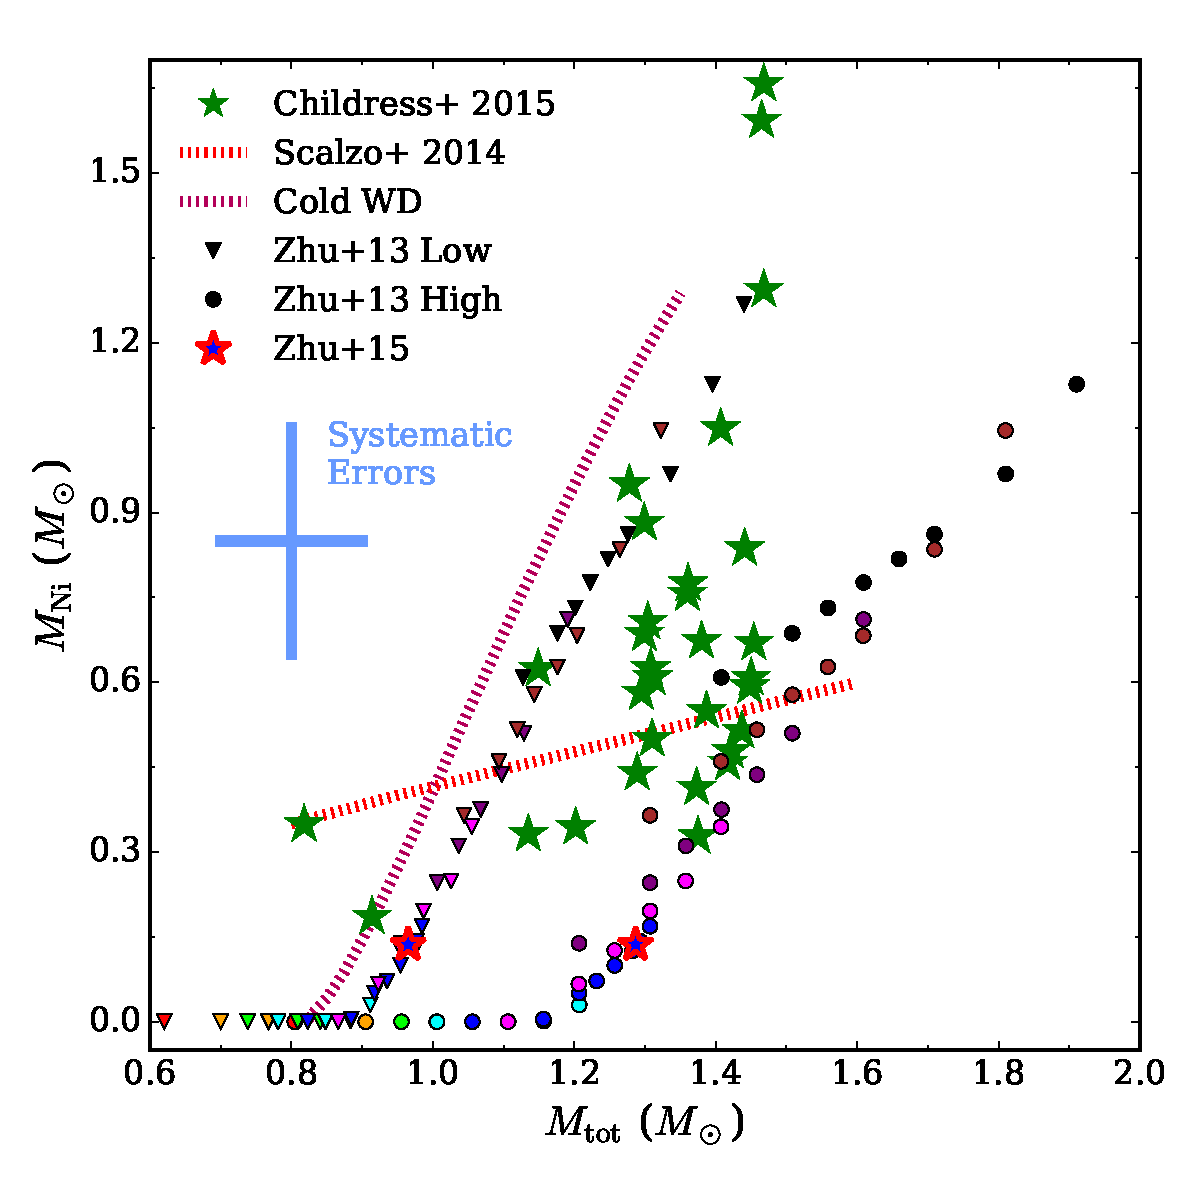
\includegraphics[angle=0,width=0.8\columnwidth]{conclusion/figures/c_MNi.pdf}
\caption{Relationships between total ejected mass \Mtot\ and synthesized \Ni\ mass \MNi\ for the merger remnants of Fig. \ref{fig:c2_pmevolution} if they were to (artificially) experience a pure detonation immediately after their estimated viscous spin-down.  \MNi\ is estimated by the mass of all remnant material with density $\rho>10^7\,\gcc$, $M(\rho>10^7)$.  \Mtot\ is estimated as the total mass of the remnant for the points, but we also extend lines leftward from each point to indicate how much of \Mtot\ is in the tenuous envelope.  Colors indicate accretor mass, as in Fig. \ref{fig:c2_constacc}.  Also plotted is the estimate for the \arepo\ MHD $0.625 - 0.65\,\Msun$ remnant (Ch. \ref{ch:ch4}; red-blue star).  All other features are as in Fig. \ref{fig:c5_mni}.}
\label{fig:c6_mcmce_mni}
\end{figure}

If powerful magnetic fields can indeed completely suppress convection, this will, at best, prevent any changes in the temperature and density structure of the WD once nuclear burning is lit.  If we assume this is the case, we can estimate the nucleosynthetic yields of our sub-\Mch\ merger remnants.  In Fig. \ref{fig:c6_mcmce_mni}, we show the total ejected mass \Mtot\ and synthesized \Ni\ mass \MNi\ of all the post-viscous remnants generated by the simple post-merger viscous evolution estimate in Sec. \ref{ssec:ch2_viscevo_possiblespindown} -- regardless of whether or not they are predicted to ignite nuclear burning -- if they were to detonate with no change to their structure.  \MNi\ is estimated by the mass of remnant material with density $\rho>10^7\,\gcc$.  It is not obvious how much of the tenuous post-viscous envelope should be included when estimating \Mtot, since some of it might have been ejected out to large distances.  We assume \Mtot\ is the total mass of the merger remnant for the points in Fig. \ref{fig:c6_mcmce_mni}, but from each point extend lines leftward by the mass of the envelope to bracket its inclusion.

Keeping in mind that our simple estimate tends to overestimate the amount of compression during viscous evolution, particularly for similar-mass mergers (Sec. \ref{sec:c2_postscript}), we see that only mergers with $\Mtot \gtrsim \Mch$ produce more than $\sim0.2\,\Msun$ of \Ni.  Since more realisitic simulations of viscous evolution predict less core compression, and not all remnants will ignite fusion, Fig. \ref{fig:c6_mcmce_mni} estimates the upper limit of \Ni\ produced by the sub-\Mch\ merger channel, and poses a challenge to its viability for producing normal SNe Ia.

\section{What are the Outcomes of CO WD Mergers?}

Considering the number of hurdles above, it appears that mergers of two CO WDs whose total mass is substantially below \Mch, including our fiducial $0.625 - 0.65\,\Msun$ merger, are unlikely to produce normal SNe Ia.  The more massive among them may ignite carbon burning, but these will probably become partly non-degenerate and expand before they achieve dynamical burning, eventually transforming their composition to O and Ne before cooling to become massive, highly-magnetized WDs.  Similar-mass super-\Mch\ WDs, on the other hand, may follow \citeal{vkercj10}'s evolutionary channel to ignite highly degenerate nuclear burning and eventually explode: mergers with accretors of $\gtrsim0.8\,\Msun$ create remnants that easily ignite nuclear burning during post-merger evolution and satisfy both the mass and central density constraints suggested by our simmering study.  Moreover, our rough estimate in Fig. \ref{fig:c6_mcmce_mni} shows their would produce \Ni\ masses consistent with normal SNe Ia.  This scenario for producing SNe Ia super-\Mch\ mergers is qualitatively different from the traditional one of slow accretion in eg. \cite{nomoi85} and \cite{yoonpr07}, though we cannot rule out the possibility of dissimilar-mass super-\Mch\ merger remnants avoiding off-center ignition and eventually cooling and compressing enough during thermal evolution \citep{shen+12} to start core pycnonuclear fusion.  Limiting explosion candidates to super-\Mch\ systems also leads to the same issue of rates that affects all other scenarios that require extremely massive WDs (Sec. \ref{ssec:c1_old_typeia}).

These super-\Mch\ binary systems, however, may have have already exploded in a violent merger (Sec. \ref{ssec:c1_new_typeia}), or shortly after coalescence due to accretion-heating from an $m = 1$ spiral mode \citep{kash+15}.  The minimum masses required for either is not well-known (see \citealt{dan+12, sato+16} for recent estimates for violent mergers), so it remains a task for future parameter-space merger studies to constrain them.
 
\section{Observational Avenues of Exploration}

Finally, we stress the potential of observational work in shedding light on this subject.  Recently revealed properties of the hot DQ population tantalizingly suggest they represent double CO WD merger remnants that did not explode.  Many of their fundamental properties, such as their masses and space density, remain poorly understood, but the Gaia mission will be able to provide parallaxes to help constrain these values \citep{dunl15thesis}.  Future observations will allow us to judge more confidently whether hot DQs are merger remnants.  If they are, the population's properties will serve as an observational check for the theoretical evolutionary scenarios in this work.

It may also be possible to spot merger remnants during their thermal evolution phase described in Sec. \ref{sec:c2_postscript}.  \cite{schw+16} consider the observable properties of their $1.5\,\Msun$ merger remnant, and calculate that it radiates on the order the Eddington luminosity for a $1.5\,\Msun$ star ($\sim10^5\,\Lsun$), and may also generate clouds of dust in its outermost layers, which will be launched as an optically thick wind.  This drives the remnant's photosphere out to $\sim10^{15}\,\mrm{cm}$, with a corresponding photospheric temperature of $\sim500\,\mrm{K}$, as well as possibly RCrB-like variablility of the remnant's luminosity.  \citep{schw+16} notes these features are similar to those of extreme AGB stars (eg. \citealt{blum+06}), and perhaps can be discovered using the same observational techniques.  Since sub-\Mch\ remnants have the same order of magnitude total energy as \Mch\ ones, their observed properties will be similar.

{\charles We have not yet modeled explosions of post-viscous merger remnants to determine if they photometrically and spectroscopically resemble SNe Ia.  Since they feature a sub-Keplerian disk through most of their evolution, and an extended envelope once they have ignited, they may look very different from typical SNe Ia.  See raskin's tamped explosions, kashyap's explosions, possibly talk about early UV flashes, Levanon's esetimates, etc.}

These new observational studies, alongside the theoretical and numerical discussed earlier, may clarify many of the outstanding questions posed throughout this thesis.  With luck, they will also lead to a clearer understanding of the fates of CO WD merger products, and SNe Ia.

%-resummarize all papers
%-don't say what we used to think

%-MRI growth rate in remnant?
%-simulation code does matter for post-merger evolution (hydrodynamic waves, magnetic fields)
%-They note that the luminosity of the nuclear burning zone is almost entirely carried away by neutrino losses (as the burning zone sits at the $\taucc = \taunu$ line), and so the remnant's source of luminosity is the heat from the merger and viscous evolution.

%\section{Does the \citeal{vkercj10} Channel Work?}

%Even if we assume runaways are vertical, the typical spun-down remnant still doesn't get to 1e7 gcc!

%%This result poses a problem for the \citeal{vkercj10} sub-\Mch\ merger channel.  \cite{shen+12} finds further compression could occur during the subsequent \textit{thermal} evolution of the remnant over $\gtrsim10^4\,\mrm{yr}$, which may allow more remnants to reach higher central density and enclose more mass within their cores.  Whether central burning could still begin is uncertain, however, since thermal diffusion and neutrino-driven cooling may favor off-center carbon ignition, or simply net cooling, even for those post-viscous remnants that are initially $\gtrsim5\times10^8\,\mrm{K}$ at their center.  Moreover, remnants, with radiation-dominated and highly magnetized carbon atmospheres, will likely drive strong outflows during their thermal evolution, further complicating predictions.  We note one advantage for delaying the explosion to during thermal evolution is the removal of the ``clutter'' of the $\gtrsim0.1\,\Msun$ hot envelope surrounding the core and extending out to $\gtrsim10^{11}\,\mrm{cm}$ \citep{shen+12}.  This imparts signatures onto the explosion not seen in ordinary SNe Ia, such as a double-peaked light curve from the shock cooling of the envelope, excess blue and UV emission prior to peak light, and a slow-decaying light curve near peak light \citep{frye+10,levasg15,pirom15}.  While \cite{shen+12}'s simulation suggests thermal evolution will do little to alter the overall structure of the envelope \citep{pirom15}, it does not account for mass loss due to winds.  These will significantly alter the size and structure of the envelope, perhaps mitigating its effects on any eventual explosion.  Meanwhile, material ejected from the remnant (both during its viscous and subsequent thermal phases) moving at the escape velocity will approach $\sim10^{17}\,\mrm{cm}$ after $\sim10^4\,\mrm{yr}$.  Interaction between this material and light from the supernova could explain \citep{shen+12, ji+13} observations of SN Ia-CSM interactions such as time-variable NaID lines (eg. \citealt{pata+07, simo+09}).

%% Magnetic coupling between the outflow and the remnant will aid in its spindown and possibly generate non-local heating through magnetic resistivity.

%Is the classic Mch DD channel even possible?

%-
%-





%\section{Observable Counterparts to Mergers}

%\section{The Evolution and Appearance of Quiescent Merger Remnants}

%% Shen+12 gives the escape velocity at 10^13 cm as 60 km/s.  Given 10^4 years of evolution, this wind could transport material to 10^18 cm, possibly explaining the variable sodium emission.

%\section{The Influence of Merger Remnants Properties on Potential Explosions}

%If sub-\Mch\ CO WD merger remnants indeed trigger thermonuclear detonations following post-merger viscous evolution, will these explosions resemble SNe Ia?  As noted in the introduction, SNe Ia observations and radiative transfer models for explosions are now sophisticated enough to distinguish fine details between different progenitors.  This question has been taken up by a number of theorists \citep{frye+10, shen+12}  Shen+12 conclusions!

%\cite{frye+10} and \cite{rask+14} do simulations

%\begin{itemize}
%	\item What are the mass loss rates of non-explosive mergers due to carbon dust superwind?  can we estimate?  could it possibly lead to Kepler's 0.6Msun oxygen WD? Shen+12 (Just under Eqn. 7) note that mass loss in radiation-dominated H/He-deficient envelopes is poor. %http://adsabs.harvard.edu/abs/2016Sci...352...67K
%	\item Near-eddington carbon burning star?  See Sec. 4 paragraph 1 of Shen+12.
%	\item Discussion with Marten: while we can't rule out further compression leading to nuclear burning during the thermal evolution phase, a combination of magnetically and Eddington-launched outflows will make the surroundings very messy - write more about this in SN Ia appearance stuff.
%	\item Importance of Ia-CSM stuff?  Shen+12 and Ji+13 (Sec. 2.2.3) have extensive sections on it.
%	\item Ji+13 has a mean magnetic field of 2e8 G; what does our simulation have?  They also (bottom of pg 7) give a quick estimate for magnetic lifetime.
%	\item What's the difference between a ring of material at $10^{13}$ cm and a continuous envelope that ends at the same radius?  Does one resemble Ia-CSM interaction, but the other lead to Fryer+10 or Piro+15 early time brightening?
%	\item Even super chandra DD systems will be much less dense than their WD binary progenitors - consequences for explosions?
%\end{itemize}



%\section{Avenues for Future Exploration}


%\subsection{Future Simulations of Mergers and Post-Merger Evolution}

%Do we need to simulate more merging WDs, especially using novel magnetohydrodynamic schemes?  Ch. STUFF suggests that the hydrodynamics up to coalescence and overall remnant properties do not substantively change when transitioning from simulating with a traditional variant of SPH to doing so with a modern moving mesh code, and getting the initial conditions (eg. synchronization, accurate tidal bulges for the onset of mass transfer) right is likely to be more important.  We await results from the the Eulerian grid WD merger simulations of \citep{katz+16} for further confirmation.

%What does require further work is the magnetic evolution during the merger, as well as the early phase of post-merger evolution and further magnetic field growth following coalescence.  The former has been insufficiently investigated with the latest generation of MHD codes, which may end up predicting very different field configurations (and possibly energies) than our exploration of the problem with \arepo.  The latter, however, is not only also poorly explored (only one group has conducted a full MHD simulation!) but essential to better understanding post-merger evolution.  This regime is particularly challenging for codes, since it requires the code minimize numerical hydrodynamic and magnetic viscosity (traditionally problematic for SPH codes) while maintaining conservative quantities -- particularly angular momentum -- over hundreds of dynamical times (traditionally difficult for grid codes).  Moreover, the problem is stiff, since evolution occurs both on a dynamical (with spiral waves) and viscous timescale, and thus quite computationally intensive.  We note the recent introduction of two codes: duffel's and hopkins', that could potentially bridge the gap.

%Arepo MHD doesn't do a good job of conserving angular momentum - balance plot shows it spurious gains it.  May be due to divergence cleaning (hopkins 16)


%Simulations of detonations within violent mergers (eg. \ref{pakm+10, bull+16, krom+16}) or mergers shortly after coalescence \citep{rask+14,vros+15}, do not reproduce the light curves and spectra of SNe Ia.  

%OUR REMNANTS AREN'T RADIATION DOMINATED.  Prad/Pion \propto T^3/\rho \propto \rho in adiabatic envelopes; we're in general much colder for any given density than Shen+12, so in fact we don't have radiation dominated envelopes, but we still have extended ones!

%Shen+16 is important, since nuclear burning energy doesn't get to exterior before 1e4 years are up, so non-burning remnants will look similar!

%It may also be possible to spot merger remnants during their thermal evolution phase described in Sec. \ref{sec:c2_postscript}.  \cite{schw+16} consider in depth the observable properties of their $\1.5\,\Msun$ merger remnant undergoing carbon and neon burning.  They note that the luminosity of the nuclear burning zone is almost entirely carried away by neutrino losses (as the burning zone sits at the $\taucc = \taunu$ line), and so the remnant's source of luminosity is the heat from the merger and viscous evolution.  Since sub-\Mch\ remnants have the same order of magnitude total energy as \Mch\ ones, their observed properties will be similar.  \cite{schw+16} find that, with an envelope and a radiation-dominated hot atmosphere of $10^{12}-10^{13}\,\mrm{cm}$, the remnant initially radiates of order the Eddington luminosity for a $1.5\,\Msun$ star ($\sim10^5\,\Lsun$) and has a photospheric temperature ranging from $4000 - 10^5\,\mrm{K}$.  The remnant may also generate clouds of dust in their outermost layers, which will then be launched as an optically thick wind, driving the remnant's photosphere out to $\sim10^{15}\,\mrm{cm}$, with corresponding photospheric temperatures of $\sim500\,\mrm{K}$, and lead to RCrB-like variablility in the remnant's luminosity.  \citep{schw+16} notes these features are similar to those of extreme AGB stars (eg. \citealt{blum+06}).

%krom+16 http://adsabs.harvard.edu/doi/10.1093/mnras/stw962
%bull+16 http://adsabs.harvard.edu/abs/2016MNRAS.455.1060B
%vros+15 http://adsabs.harvard.edu/abs/2015arXiv151004286V
%papi+15 http://adsabs.harvard.edu/abs/2015MNRAS.449..942P
%pirom15 http://adsabs.harvard.edu/abs/2015arXiv151203442P



%% This adds a line for the Bibliography in the Table of Contents.
\addcontentsline{toc}{chapter}{Bibliography}
%% *** Set the bibliography style. ***
%% (change according to your preference/requirements)
\bibliographystyle{apj}
%% *** Set the bibliography file. ***
%% ("thesis.bib" by default; change as needed)
\bibliography{AutoBibliography}

%% *** NOTE ***
%% If you don't use bibliography files, comment out the previous line
%% and use \begin{thebibliography}...\end{thebibliography}.  (In that
%% case, you should probably put the bibliography in a separate file and
%% `\include' or `\input' it here).

\end{document}

%%%%%%%%%%%% REFERENCE ADS HANDLES %%%%%%%%%%%
%%% Categorized, then sorted alphabetically

%%%% Core works (includes Marten's) %%%%
%citation{vkercj10}{2010ApJ...722L.157V}	% vKCJ channel
%citation{vker13}{2013RSPTA.37120236V}
%citation{zhu+13}{2013ApJ...767..164Z}
%citation{zhu+15}{2015ApJ...806L...1Z}
%citation{pakm+16}{2016MNRAS.455.1134P}		% Improving Arepo

%%%% Code papers %%%%
%citation{ager+07}{2007MNRAS.380..963A} 	% SPH instability failure paper
%citation{bals95}{1995JCoPh.121..357B} 		% balsara switch
%citation{chaw16}{2016MNRAS.458..480C} 		% Godunov SPH
%citation{culld10}{2010MNRAS.408..669C}		% critique of time-dependent alpha viscosity
%citation{dehna12}{2012MNRAS.425.1068D} 	% SPH pair-generating instability
%citation{dedn+02}{2002JCoPh.175..645D}		% dedner divergence cleaning
%citation{dola+05}{2005MNRAS.364..753D} 	% time-dependent alpha viscosity
%citation{duffm11}{2011ApJS..197...15D}		% TESS
%citation{dube+09}{2009arXiv0903.4875D}		% FLASH update
%citation{evanh88}{1988ApJ...332..659E}		% constrained transport
%citation{floc+10}{2010A&A...516A..26F}		% test of MRI simulations across wide range of codes
%citation{fryx+00}{2000ApJS..131..273F}		% Flash paper
%citation{gabujl12}{2012ApJ...758..103G} 	% another moving mesh code
%citation{gingm77}{1977MNRAS.181..375G}		% SPH origin paper 1
%citation{gove+15}{2015MNRAS.448..792G} 	% GASOLINE chaNGa
%citation{haye+06}{2006ApJS..165..188H}		% ZEUS-MP2 paper
%citation{hernk89}{1989ApJS...70..419H}		% Gasoline's kernel
%citation{hesss10}{2010MNRAS.406.2289H}		% SPH surface tension
%citation{hopk13}{2013MNRAS.428.2840H}		% pressure-entropy formulation of SPH
%citation{hopk15}{2015MNRAS.450...53H}		% Gizmo paper
%citation{hopkr16}{2016MNRAS.455...51H}		% divergence cleaning for Gizmo MHD
%citation{hu+14}{2014MNRAS.443.1173H}		% modern pressure-entropy SPH
%citation{kell+14}{2014MNRAS.442.3013K} 	% updates to hydro schemes for Gasoline2
%citation{kell+15}{2015MNRAS.453.3499K}		% Gasoline 2
%citation{lucy77}{1977AJ.....82.1013L}		% SPH origin paper 2
%citation{miyok05}{2005JCoPh.208..315M} 	% HLLD Solver
%citation{moczvh14}{2014MNRAS.442...43M}	% constrained transport in unstructured grid
%citation{mocz+16}{2016arXiv160602310M}		% arepo's CT solver
%citation{mona05}{2005RPPh...68.1703M}		% Monaghan SPH review
%citation{morrm97}{1997JCoPh.136...41M}		% time-dependent alpha viscosity
%citation{pakmbs11}{2011MNRAS.418.1392P}	% ruediger's original magnetic fields paper
%citation{pakms13}{2013MNRAS.432..176P}		% ruediger's galactic magnetic fields paper
%citation{paxt+11}{2011ApJS..192....3P}		% MESA paper
%citation{paxt+13}{2013ApJS..208....4P}		% MESA paper 2
%citation{paxt+15}{2015ApJS..220...15P}		% MESA paper 3
%citation{powe+99}{1999JCoPh.154..284P}		% powell's divergence cleaner CHECKED
%citation{pric08}{2008JCoPh.22710040P}		% artificial entropy mixing in SPH
%citation{readha10}{2010MNRAS.405.1513R}	% E0 and surface tension issues with SPH
%citation{ross09}{2009NewAR..53...78R}		% rosswog's sph review
%citation{shen+10}{2010MNRAS.407.1581S} 	% Gasoline's new thermal diffusion term
%citation{spri05}{2005MNRAS.364.1105S} 		% Gadget2
%citation{spri10rev}{2010ARA&A..48..391S}	% volker SPH review
%citation{spri10}{2010MNRAS.401..791S}		% AREPO
%citation{tamb+15}{2015MNRAS.453.2490T} 	% Gasoline 2
%citation{timms00}{2000ApJS..126..501T}		% Helmholtz EOS paper
%citation{toth00}{2000JCoPh.161..605T}		% divergence cleaning overview
%citation{tric15}{2015AAS...22521106T}		% Terry's talk comparing MHDSPH to Arepo
%citation{vandr16}{2016A&C....16..109V}		% SHADOWFAX moving mesh code
%citation{voge+12}{2012MNRAS.425.3024V}		% arepo explicit refinement for maintaining fixed mass
%citation{wadssq04}{2004NewA....9..137W}	% Gasoline paper

%%%% Explosion modeling %%%%
%citation{fink+07}{2007A&A...476.1133F} 	% fink's ddet paper
%citation{fink+10}{2010A&A...514A..53F}		% fink's d-det work
%citation{frye+10}{2010ApJ...725..296F}		% Fryer double degenerate light curves.
%citation{holc+13}{2013ApJ...771...14H}		% holcomb's He hotspot detonation
%citation{mazumw77}{1977ApJ...213..518M}	% mazurek early work on detonations
%citation{rask+14}{2014ApJ...788...75R}		% Cody's tamped explosion models.
%citation{seit+09}{2009ApJ...696..515S}		% seitenzahl detonation paper
%citation{seitcr11}{2011MNRAS.414.2709S}	% dtd
%citation{shig+92}{1992ApJ...386L..13S}		% sub-Ch -> right nucleosyn/energetics
%citation{shenb14}{2014ApJ...785...61S}		% converging shocks in ddets
%citation{shenm14}{2014ApJ...797...46S}		% conditions for He detonation
%citation{sim+10}{2010ApJ...714L..52S}		% stuart's zero-temperature pure detonations
%citation{woos+09}{2009ApJ...704..255W}		% deflagration, density effects
%citation{woos+11}{2011ApJ...734...37W}		% ...

%%%% WD merger theory/sim papers %%%%
%citation{benz+90}{1990ApJ...348..647B}		% benz's early SPH work
%citation{brow+16}{2016ApJ...824...46B}		% every interacting DWD may merge
%citation{burk+13}{2013MNRAS.433..332B}		% tidal resonance leads to WD corotation
%citation{dan+11}{2011ApJ...737...89D}		% dan's exact intial condition work
%citation{dan+12}{2012MNRAS.422.2417D} 		% dan's merger param space
%citation{dan+14}{2014MNRAS.438...14D} 		% dan's merger remnant param space
%citation{dan+15}{2015MNRAS.454.4411D}		% detonations in mergers
%citation{dsou+06}{2006ApJ...643..381D}		% d'souza's exact initial condition work (eulerian)
%citation{fulll12}{2012MNRAS.421..426F}		% fuller's tidal analysis for cortation
%citation{fulll14}{2014MNRAS.444.3488F}		% follow-up to fulll12
%citation{gokhpf07}{2007ApJ...655.1010G}	% update to marsns04
%citation{guerig04}{2004A&A...413..257G}	% guerrero's 2004 sims
%citation{kash+15}{2015ApJ...800L...7K}		% rahul, ji and bob's work on spiral waves in remnants 
%citation{katz+16}{2016ApJ...819...94K} 	% katz and zingale work on amr WD mergers
%citation{kremsk15}{2015ApJ...806...76K}	% update to marsns04
%citation{lairs94}{1994ApJ...437..742L}		% compressible ellipsoid models of wd binaries
%citation{loreig09}{2009A&A...500.1193L}	% loren-aguilar's sims
%citation{loreig10}{2010MNRAS.406.2749L} 	% loren-aguilar's collision work
%citation{lubos75}{1975ApJ...198..383L}		% transition from disk to direct impact accretion
%citation{marsns04}{2004MNRAS.350..113M}	% marsh's merger mass trans stability
%citation{mochl89}{1989A&A...209..111M}		% turbulent viscosity synchronization of WD binaries
%citation{moll+14}{2014ApJ...785..105M}		% Part 1 of Cody et al's recent merger work
%citation{pakm+10}{2010Natur.463...61P}		% Ruediger's violent mergers - subluminous
%citation{pakm+11}{2011A&A...528A.117P}		% Ruediger's violent mergers - dissimilar mass
%citation{pakm+12}{2012ApJ...747L..10P}		% Ruediger's violent mergers - normal Ia
%citation{pakm+12sph}{2012MNRAS.424.2222P}	% Stellar gadget (also approximate vs accurate ics)
%citation{pakm+13}{2013ApJ...770L...8P} 	% ruediger's helium detonation in violent mergers
%citation{piro11}{2011ApJ...740L..53P}		% tony's work on tides in WD binaries
%citation{rask+12}{2012ApJ...746...62R}		% Cody's work
%citation{segrcm97}{1997ApJ...481..355S}	% segretain's early SPH mergers
%citation{shen15}{2015ApJ...805L...6S}		% every interacting DWD may merge
%citation{uryue98}{1998ApJS..118..563U}		% equilibrium solution for corotating wd binary
%citation{verbr88}{1988ApJ...332..193V}		% WD mass transfer stability
%citation{yoonpr07}{2007MNRAS.380..933Y}	% Yoon's massive WD sim + post-merger work (1D sub-Edd)

%%%% WD post-merger evolution %%%%
%citation{ji+13}{2013ApJ...773..136J}		% ji and bob's MHD PME work, shows ignition
%citation{nomoi85}{1985ApJ...297..531N}		% nomoto's old slow accretion sim
%citation{schw+12}{2012MNRAS.427..190S}		% josiah's post merger stuff
%citation{schw+16}{2016arXiv160602300S}		% josiah's thermal evolution stuff.
%citation{shen+12}{2012ApJ...748...35S}		% ken's semi-analytical work

%%%%%% Convection and (rot/mag) simmering %%%%%%%
%citation{augubt16}{2016arXiv160303659A} 	% augustson massive star convection
%citation{barkdl14}{2014ApJ...791...13B}	% Barker's simulation of rotating RB convection and comparison to Stevenson's derivation
%citation{brunbt05}{2005ApJ...629..461B}	% brun A-star convection
%citation{chabgb07}{2007A&A...472L..17C} 	% Chabrier et al.'s inclusion of magnetic fields
%citation{feat+09}{2009ApJ...705.1000F} 	% featherston's magnetic dynamo action in A stars; having fossil fields amplifies saturation field to superequipartition
%citation{feidc12}{2012ApJ...761...30F} 	% Feiden & Chaboyer's magnetic fields method
%citation{garcw95}{1995ApJ...454..895G}		% Garcia-Senz and Woosley's floating burning bubbles
%citation{gougt66}{1966MNRAS.133...85G} 	% Gough & Taylor's original variational formulation
%citation{kuhlwg06}{2006ApJ...640..407K}	% kuhlen's hydro convection sims
%citation{lesa+06}{2006MNRAS.368..187L}		% lesaffre's semi-analytical work, notable for using t_conv = alpha*t_h as their stopping point
%citation{macdm09}{2009ApJ...700..387M} 	% Macdonald & Mullan's application of GT66 to brown dwarfs; includes degeneracy term
%citation{maed09}{2009pfer.book.....M}		% Maeder's book on stellar rotation
%citation{maed+13}{2013A&A...553A...1M}		% Maeder's paper on general instability criteria
%citation{mullm01}{2001ApJ...559..353M} 	% Mullan & Macdonald's application of GT66 to M-dwarfs
%citation{nona+12}{2012ApJ...745...73N}		% nonaka's hydro convection sims
%citation{piro08}{2008ApJ...679..616P}		% piro's work on rotating runaway WDs
%citation{pirob08}{2008ApJ...673.1009P}		% some stuff on neutronization
%citation{piroc08}{2008ApJ...678.1158P}		% piro & phil's work
%citation{procw82}{1982RPPh...45.1317P} 	% proctor and weiss's review on magnetoconvection
%citation{saion04}{2004ApJ...615..444S}		% Saio & Nomoto's accreting WD
%citation{seit+13}{2013MNRAS.429.1156S}		% seitenzahl's work on delayed det where ignition points are varied
%citation{steiw06}{2006ApJ...643.1190S}		% stein & wheeler's convective urca sim work
%citation{stev79}{1979GApFD..12..139S} 		% Stevenson 1D formulation for magnetic and rotational suppression of convection.
%citation{tass00}{2000stro.book.....T} 		% Tassoul's variational derivation of the SH criterion
%citation{wooswk04}{2004ApJ...607..921W}	% wwk04
%citation{zing+09}{2009ApJ...704..196Z}		% zingale's hydro convection sims
%citation{zing+11}{2011ApJ...740....8Z}		% same, but with rotation

%%%% Other simulations (pop synth) %%%%
%citation{abdi+10}{2010PhRvD..81d4012A} 	% GR simulation of AIC
%citation{brig+15}{2015MNRAS.447.1713B}		% brigg's population synthesis for HFMWDs CHECKED
%citation{hayw+14}{2014MNRAS.442.1992H}		% Galaxy mergers in Arepo
%citation{marips14}{2014MNRAS.437.1750M}	% Galaxy formation in cosmo sims
%citation{mitc+09}{2009MNRAS.395..180M}		% SPH/Eulerian code comparison for galaxy cluster formation
%citation{nele+01}{2001A&A...368..939N}		% pop synth for detached WD binaries for AM CVn systems
%citation{nele+01a}{2001A&A...365..491N}	% as above, except for close detached WD binaries
%citation{ohlm+16}{2016ApJ...816L...9O}		% common envelope Arepo sim
%citation{ruitbf09}{2009ApJ...699.2026R}	% Ruiter population synthesis
%citation{tracsp07}{2007MNRAS.377..997T}	% SPH/Eulerian code comparison for stellar collisions
%citation{woosk11}{2011ApJ...734...38W}		% woosley double detonation minimum He mass

%%%% Magnetic growth theory papers %%%%
%citation{balbh91}{1991ApJ...376..214B}		% MRI paper
%citation{garc+12}{2012ApJ...749...25G}		% garcia-berro et al. on white dwarf mergers generating strong magnetic fields
%citation{giac+15}{2015ApJ...809...39G}		% giacomazzo's application of zrake & macfayden's work
%citation{dionar15}{2015PhRvD..92h4064D}	% dionysopoulou's work, which shows a much reduced field growth compared to giac+14
%citation{kiuc+14}{2014PhRvD..90d1502K}		% kiuchi's run - higher resolution than the giacomazzo group, and slightly greater amplification 
%citation{kule+13}{2013MNRAS.431.2778K}		% kulebi's disk/remnant coupling model, which attempts to predict final HFMWD 
%citation{oberam10}{2010A&A...515A..30O}	% obergaulinger's study on turbulent MHD dynamo
%citation{pricr06}{2006Sci...312..719P}		% price and rosswog's MHDSPH NS simulation - note pric12 states this simulation is WRONG
%citation{pric12}{2012JCoPh.231..759P} 		% price's 2012 SPH review
%citation{spru02}{2002A&A...381..923S}		% Tayler-Spurit paper
%citation{wicktf14}{2014MNRAS.437..675W}	% wickramasinghe's simple dynamo estimate
%citation{zrakm13}{2013ApJ...769L..29Z}		% zrake and macfayden's turbulent MHD dynamo

%%%%%%%%%% Spiral wave theory & sim %%%%%%%%%%%
%citation{adamrs89}{1989ApJ...347..959A}	% adams's work on the SLING instability around YSOs
%citation{balb03}{2003ARA&A..41..555B}		% spiral wave review
%citation{cent+01}{2001ApJ...550L.193C}		% Low T/W m = 1 instability in differentially rotating stars
%citation{dval+06}{2006MNRAS.370..529D}		% planet migration code comparison
%citation{east+16}{2016PhRvD..93b4011E}		% follow-up to pasc+15
%citation{hopkq10}{2010MNRAS.407.1529H}		% hopkins work on smbh accretion
%citation{hopk10}{2010arXiv1009.4702H}		% follow-up to hopkq10
%citation{kratl16}{2016arXiv160301280K}		% kaitlin's review paper on grav instability
%citation{lin15}{2015MNRAS.448.3806L}		% min-kai on thermal-based grav instability in disks
%citation{merub10}{2010MNRAS.406.2279M}		% self-gravitating disk sph simulation
%citation{muhl+14}{2014PhRvD..90j4014M}		% muhlberger's magnetized T/W instability simulation
%citation{ott+05}{2005ApJ...625L.119O}		% m = 1 spiral in post-bounce SN core
%citation{papap84}{1984MNRAS.208..721P}		% p&p instability
%citation{pasc+15}{2015PhRvD..92l1502P}		% spiral mode in NS-NS merger remnant (GR-AMR code)
%citation{ricela05}{2005MNRAS.364L..56R}	% self-gravitating disk sph simulation
%citation{rogew12}{2012MNRAS.423.1896R}		% self-gravitating disk sph simulation in Gasoline
%citation{saijbs03}{2003ApJ...595..352S}	% Follow-up to cent+01
%citation{shu+90}{1990ApJ...358..495S}		% follow-up to adamrs89
%citation{radibo16}{2016arXiv160305726R}	% spiral mode in NS-NS merger remnant (GR-AMR code)
%citation{wattaj05}{2005ApJ...618L..37W}	% T/W instability

%%%%%% Population statistics and DTDs %%%%%%%%%%
%citation{chil+15}{2015MNRAS.454.3816C} 	% childress's M_56 vs M_tot relationship paper
%citation{klei+13}{2013ApJS..204....5K}		% SDSS DR7 WD catalog, has mass distribution
%citation{li+11}{2011MNRAS.412.1441L}		% lick team nearby supernova statistics
%citation{mann+05}{2005A&A...433..807M}		% mannucci sn ia rate (from NIR galaxy obs)
%citation{maozsg10}{2010ApJ...722.1879M}	% maoz dtd
%citation{menn+10}{2010ASPC..435...33M}		% mennekens dtd
%citation{prichs08}{2008ApJ...683L..25P}	% pritchet's estimate for the SN Ia/WD formation rate ratio
%citation{scalzrs14}{2014MNRAS.445.2535S} 	% scalzo's M_56 vs M_tot relationship paper
%citation{scalz+14}{2014MNRAS.440.1498S} 	% scalzo's M_tot vs stretch relation
%citation{tremb09}{2009ApJ...696.1755T}		% field WD mass distribution

%%%% Other theory papers %%%%
%citation{alth+09}{2009ApJ...693L..23A}		% Single star formation channel for hot DQs
%citation{belo14}{2014MNRAS.438..169B}		% belobodorov's semi-analytical work on post-merger evolution transients
%citation{eggl83}{1983ApJ...268..368E}		% Eggleton roche overflow radius estimate
%citation{levasg15}{2015MNRAS.447.2803L}	% levanon's estimate of effect on early light curve
%citation{pacz71}{1971ARA&A...9..183P}		% Paczynski roche overflow estimate
%citation{pirom15}{2015arXiv151203442P} 	% tony's double-peaked SN Ia due to envelope
%citation{saioj00}{2000MNRAS.313..671S}		% saio and jeffrey He - He merger
%citation{saioj02}{2002MNRAS.333..121S}		% saio and jeffrey He - CO merger
%citation{saion85}{1985A&A...150L..21S}		% edge-lit ignition
%citation{saion98}{1998ApJ...500..388S}		% saio/nomoto ONe production following merger
%citation{shaks73}{1973A&A....24..337S}		% shakura/sunyaev alpha visc

%%%% Other observational papers %%%%
%citation{aspd+11}{2011ApJ...738...94A}		% rising deflagration bubbles
%citation{badem12}{2012ApJ...749L..11B}		% Badenes and Moaz's paper on galactic WD merger rate from SDSS
%citation{bars+95}{1995MNRAS.277..971B}		% RE J 0317 
%citation{bran+06}{2006PASP..118..560B} 	% branch definition of normal SNe Ia
%citation{brow+11}{2011ApJ...737L..23B}		% eclipsing 12-min WD binary
%citation{chur+14}{2014Natur.512..406C}		% 56Co detection in ejecta
%citation{dist10}{2010ApJ...719..474D}		% di Stefano's SSS work
%citation{dufo+13}{2013ASPC..469..167D}		% Patrick's work on hot DQs 
%citation{dunlc15}{2015ASPC..493..547D} 	% bart and chris's work published in conference proceeding
%citation{gera+07}{2007ApJ...661..995G}		% slow-moving 58Ni
%citation{geroh89}{1989ApJS...70..661G}		% rapidly rotating WDs
%citation{gilfb10}{2010Natur.463..924G}		% gilfanov's SSS rates from UV backgrd
%citation{hama97}{1997IAUS..180...91H}		% [WR] wind mass loss rates
%citation{kerz+14}{2014ApJ...796L..26K}		% Wolfgang's late-time observations of positron trapping in SN Ia
%citation{khok91}{1991A&A...245..114K} 		% DDT paper
%citation{clars77}{1977hisu.book.....C}		% tycho's SN reference
%citation{kube+10}{2010A&A...524A..36K}		% REJ 0317
%citation{lawr+13}{2013MNRAS.433.1599L}		% Lawrie's long-period (probably spin) hot DQ
%citation{maed+10a}{2010ApJ...708.1703M}	% slow-moving 58Ni
%citation{maed+10b}{2010Natur.466...82M}	% ...
%citation{pata+07}{2007Sci...317..924P}		% patat's NaID work
%citation{phil93}{1993ApJ...413L.105P}		% phillips relation
%citation{ruizs98}{1998ApJ...500..360R}		% Ruiz-Lapuente's work on positron trapping due to magnetic fields
%citation{ruiz04}{2004ApJ...612..357R}		% tycho's SN
%citation{simo+09}{2009ApJ...702.1157S}		% Simon's Na ID paper
%citation{stei+10}{2010ApJ...716L.146S}		% eclipsing detached WD binary
%citation{taub+09}{2011MNRAS.412.2735T}		% slow-moving superchandrasekhar
%citation{will+13}{2013ApJ...769..123W}		% Williams's DQ paper (though this one is a "warm DQ")

%%%% SN Ia review papers %%%%
%citation{fili97}{1997ARA&A..35..309F}		% optical spectra of SNe Ia
%citation{hilln00}{2000ARA&A..38..191H}		% wolfgang hillebrandt's 2000 work
%citation{hill+13}{2013FrPhy...8..116H}		% hillebrandt's recent SN Ia review paper
%citation{howe11}{2011NatCo...2E.350H}		% howell's SN Ia review paper
%citation{maozmn14}{2014ARA&A..52..107M}	% Maoz's review paper
%citation{tsebs15}{2015MNRAS.447.2568T}		% not a review, but excellent introduction
%citation{vker12}{2012arXiv1206.1605V}		% marten's review of Mch problems

%%%% Gravitational Wave Stuff %%%%%
%citation{amar+13}{2013GWN.....6....4A}		% eLISA
%citation{ligo+15}{2015CQGra..32g4001L}		% aLIGO
%citation{mars11}{2011CQGra..28i4019M}		% Marsh's primary on GW DWDs
%citation{neleyp01}{2001A&A...375..890N}	% Nelemans' GW estimate

%%%% Misc/General %%%%
%citation{andrpt06}{2006ApJ...646.1160A}	% andronov theoretical model for blue straggler formation
%citation{chan31}{1931ApJ....74...81C}		% chandrasekhar mass
%citation{chio+15}{2015MNRAS.448.2100C}		% single WD channel to sne ia?
%citation{clay+07}{2007ApJ...662.1220C}		% clayton's earlier work on RCrBs
%citation{clay13}{2013ASPC..469..133C} 		% Clayton's review on mergers making rCB stars
%citation{distfg15}{2015arXiv150107837D}	% planets make SNe Ia
%citation{garc13}{2013IAUS..281...52G}		% enrique's review on oxygen-neon
%citation{goedp04}{2004prma.book.....G} 	% goedbloed's MHD textbook
%citation{hebe16}{2016arXiv160407749H}		% subdwarf stars
%citation{herw05}{2005ARA&A..43..435H}		% AGB and super-AGB evolution
%citation{hoylf60}{1960ApJ...132..565H}		% hoyle & fowler nucleosynthetics of SNe
%citation{ibent85}{1985ApJS...58..661I}		% iben & tutukov's exhaustive survey of stellar evolution
%citation{justph11}{2011MNRAS.410..984J}	% justham's work on sdOs
%citation{justpv14}{2014ApJ...796..121J}	% justham's merger origins of LBVs
%citation{kais+10}{2010SPIE.7733E..0EK}		% Pan-STARRS instrument paper
%citation{kippww12}{2012sse..book.....K}	% Kippehahn
%citation{knigs09}{2009Natur.457..288K}		% knigge & sills on whether blue stragglers are collisional or due to RLOF 
%citation{loke+10}{2010JPhCS.256a2026L}		% SciNet paper
%citation{ligo16}{2016PhRvL.116m1102A}		% ligo BBH-merger discovery paper
%citation{lsst09}{2009arXiv0912.0201L}		% lsst science book 2.0
%citation{marsdd95}{1995MNRAS.275..828M}	% low mass wds need friends (discusses He WD formation)
%citation{mink41}{1941PASP...53..224M}		% minkowski spectroscopic separation
%citation{moros09}{2009A&A...507.1575P}		% low-mass CO WD
%citation{nele10}{2010Ap&SS.329...25N}		% pop synth for sdB stars
%citation{nandil14}{2014ApJ...786...39N}	% nandez's SPH work on V1309 Sco
%citation{perl+99}{1999ApJ...517..565P}		% Perlmutter dark energy paper
%citation{rau+09}{2009PASP..121.1334R}		% PTF instrument paper
%citation{ries+98}{1998AJ....116.1009R}		% Riess dark energy paper
%citation{ross15}{2015IJMPD..2430012R}		% rosswog binary compact merger review
%citation{spru13}{2013arXiv1301.5572S}		% henk's MHD textbook
%citation{tyle+11}{2011A&A...528A.114T}		% tylenda's V1309 Sco paper
%citation{webb84}{1984ApJ...277..355W}		% webbink's seminal merger paper for SN Ia and He - CO -> RCB
%citation{woos99}{1999ApJ...525C.924W}		% woosley on hoyle
%citation{yung05}{2005AIPC..797....1Y}		% yungelson's overview of binary evolution and population synthesis

%ZZZitation{rappds94}{1994ApJ...426..692R}




%citation{bloo+12}{2012ApJ...744L..17B} 	% 2011fe shock breakout
%citation{nuge+11}{2011Natur.480..344N}		% 2011fe shock breakout

%citation{wheli73}{1973ApJ...186.1007W}		% first mention of SD channel
%citation{ibent84}{1984ApJS...54..335I}		% the other DD paper
%citation{townsb04}{2004ApJ...600..390T}	% nova shell mass loss
%citation{zorosg11}{2011A&A...536A..42Z}	% recurrent novae gain mass?
%citation{hachkn10}{2010ApJ...724L.212H}	% maybe SSS WDs spend time in a third phase that's optically thick?
%citation{joha+14}{2014MNRAS.442.1079J}		% counter to hachisu
%citation{idanss13}{2013MNRAS.433.2884I}	% he flashes
%citation{hill+16}{2016ApJ...819..168H}		% maybe it is possible to grow WDs despite he flashes
%citation{clae+14}{2014A&A...563A..83C}		% joke's BPS study - similar results for total SN rate
%citation{maoz+11}{2011MNRAS.412.1508M}		% Maoz estimate of total SN rate
%citation{schwqb15}{2015MNRAS.453.1910S}	% Schwab's AIC work
%citation{bran98}{1998ARA&A..36...17B}		% Branch normal definition (see also bran+06)
%citation{arne96}{1996sunu.book.....A}		% Arnett's book on nucleosynthesis
%citation{stri+06}{2006A&A...450..241S}		% 56Ni yields
%citation{fishj15}{2015ApJ...805..150F}		% bob's overluminous Mch
%citation{phil+07}{2007PASP..119..360P}		% SNe IaX pure deflagration
%citation{krom+13}{2013MNRAS.429.2287K}		% SNe IaX pure deflagration
%citation{fink+14}{2014MNRAS.438.1762F}		% SNe IaX pure deflagration
%citation{sull+10}{2010MNRAS.406..782S}		% Sn Ia host galaxy dependence
%citation{hamu+00}{2000AJ....120.1479H}		% Sn Ia host galaxy dependence
%citation{xavi+13}{2013MNRAS.434.1443X}		% Sn Ia host galaxy dependence
%citation{li+02}{2003PASP..115..453L}		% 2002cx
%citation{fole+13}{2013ApJ...767...57F}		% 2002cx type
%citation{mazz+97}{1997MNRAS.284..151M}		% 1991bg
%citation{yama+09}{2009ApJ...707L.118Y}		% 2009dc
%citation{nielvn13}{2013MNRAS.435..187N}	% pre-explosion companion search
%citation{li+11cpn}{2011Natur.480..348L}	% pre-explosion companion search of 2011fe
%citation{niel+14}{2014MNRAS.442.3400N}		% pre-explosion companion search of 2014j
%citation{kerz+14rem}{2014ApJ...782...27K}	% wolfgang's search for companions in kepler
%citation{ollms15}{2015Natur.521..332O}		% kepler telescope shock heated companion
%citation{magu+16}{2016MNRAS.457.3254M}		% maguire H and He entrained SNe
%citation{benzth89}{1989ApJ...342..986B}	% benz collisions
%citation{katzd12}{2012arXiv1211.4584K}		% three-body interactions generate SNe Ia
%citation{koza62}{1962AJ.....67..591K}		% kozai-lidov mechanism
%citation{lido62}{1962P&SS....9..719L}		% kozai-lidov mechanism
%citation{garc+13}{2013MNRAS.436.3413G}		% WD collision simulation
%citation{kush+13}{2013ApJ...778L..37K}		% WD collision simulation
%citation{seit+16}{2016arXiv160600089S}		% GCD makes 91T?
%citation{sato+16}{2016ApJ...821...67S}		% violent merger lower limits
%citation{lieb+93}{1993AJ....105..301L}		% 1991bg
%citation{illks12}{2012MNRAS.419.1695I}		% spin-down through magnetic dipole radiation
%citation{dild+12}{2012Sci...337..942D}		% PTF 11kx
%citation{soke13}{2013MNRAS.431.1541S}		% Soker's explanation for PTF 11kx
%citation{livir03}{2003ApJ...594L..93L}		% core degenerate founding paper
%citation{kashs11}{2011MNRAS.417.1466K}		% kashi & soker's CD channel
%citation{guil+10}{2010ApJ...709L..64G}		% guillochon shows you can violently ignite a He detonation in a merger

%citation{clay12}{2012JAVSO..40..539C}		% R CrB
%citation{jeff14}{2014IAUS..301..297J}		% EHe stars

%citation{wald+11}{2011ApJ...738...21W}		% He shell explosions
%citation{shen+10he}{2010ApJ...715..767S}	% He shell explosions
%citation{pere+10}{2010Natur.465..322P}		% Ca-rich SN Ib transients
%citation{miya+80}{1980PASJ...32..303M}		% ONe WD collapse
%citation{marq+15}{2015A&A...580A.118M}		% ONe WD explosions
%citation{hurlpt00}{2000MNRAS.315..543H}	% 1.25 Msun CO WD (ref from marq+15)
%citation{dess+06}{2006ApJ...644.1063D}		% AIC sim
%citation{dess+07}{2007ApJ...669..585D}		% AIC sim
%citation{frye+09}{2009ApJ...707..193F}		% AIC sim
%citation{livn90}{1990ApJ...354L..53L}		% double detonation proposal
%citation{woosw94}{1994ApJ...423..371W}		% double detonation proposal
%citation{mollw13}{2013ApJ...774..137M}		% can He detonation  travel into CO core?
%citation{krom+10}{2010ApJ...719.1067K}		% DDet spectra
%citation{ropk+11}{2011PrPNP..66..309R}		% Ropke's comparison of violent mergers
%citation{pirotk14}{2014MNRAS.438.3456P}	% 56Ni distribution in context of mergers

%citation{petem63}{1963PhRv..131..435P}		% grav radiation
%citation{verb84}{1984MNRAS.209..227V}		% mag braking
%citation{knigbp11}{2011ApJS..194...28K}	% mag braking
%citation{toon+14}{2014A&A...562A..14T}		% population synthesis
%citation{toonnp12}{2012A&A...546A..70T}	% DD merger pop synth

%citation{carr+14}{2014A&A...565A..11C}		% Gaia and WDs
%citation{gaen+15}{2015arXiv150602653G}		% Gaia and WDs
%citation{gian+15}{2015ApJ...812..167G}		% ELM survey
%citation{brow+10}{2010ApJ...723.1072B}		% ELM survey paper I
%citation{napi+07}{2007ASPC..372..387N}		% SPY survey
%citation{york+00}{2000AJ....120.1579Y}		% SDSS
%citation{maozbb12}{2012ApJ...751..143M}	% prelude to badem12

%citation{trem+16}{2016arXiv160605292T}		% newest WD field distribution
%citation{liebbh05}{2005ApJS..156...47L}	% 1 Msun peak of field WD dist
%citation{giambd12}{2012ApJS..199...29G}	% 1 Msun peak of field WD dist
%citation{reba+15a}{2015MNRAS.450..743R}	% 1 Msun peak of field WD dist
%citation{reba+15b}{2015MNRAS.452.1637R}	% 1 Msun peak of field WD dist
%citation{weggp12}{2012MNRAS.426..427W}		% 1 Msun peak of field WD dist
%citation{han+02}{2002MNRAS.336..449H}		% He - He mergers

%citation{trem+15}{2015ApJ...812...19T}		% HFMWDs
%citation{garc+16}{2016IJMPD..2530005G}		% HFMWDs
%citation{kepl+13}{2013MNRAS.429.2934K}		% HFMWDs
%citation{wickf05}{2005MNRAS.356.1576W}		% HFMWDs
%citation{kisst15}{2015ApJ...809..108K}		% Yevgeni's work on PMS dynamos
%citation{ferrdg15}{2015SSRv..191..111F}	% massive maagnetic WDs
%citation{lieb+15}{2015ApJ...804...93L}		% HFMWDs need friends to form

%citation{zhanj12}{2012MNRAS.419..452Z}		% He - He merger

%citation{dufo+07}{2007Natur.450..522D}		% Hot DQs
%citation{dufo+08}{2008ApJ...683..978D}		% Hot DQs
%citation{will+16}{2016ApJ...817...27W}		% Hot DQ rapid rotation
%citation{dufo+11}{2011BaltA..20..511D}		% Really preliminary log g measurements

%citation{bild+07}{2007ApJ...662L..95B} 	% .Ias
%citation{blum+06}{2006AJ....132.2034B}		% Extreme AGB stars

%citation{lewibt16}{2016arXiv160606972L}	% SPMHD
%citation{vros+15}{2015arXiv151004286V}		% Kash+15 detonation
%citation{ries+96}{1996ApJ...473...88R}		% Color-luminosity relation

%citation{lepok13}{2013ApJ...771...13L}		% Kelly's work on rapidly accreting WDs
%citation{rask+10}{2010ApJ...724..111R}		% Raskin's collision work

%citation{soke98}{1998AJ....116.1308S}		% RGB-planet merger to make single sdB
%citation{zhanj12b}{2012MNRAS.426L..81Z}	% RCrB from He-He merger
%citation{zhan+14}{2014MNRAS.445..660Z}		% RCrB
%citation{pier+14}{2014MNRAS.445.3239P}		% He accretion
%citation{ruit+11}{2011MNRAS.417..408R}
%citation{ruit+13}{2013MNRAS.429.1425R}
%citation{ruit+14}{2014MNRAS.440L.101R}

%citation{bullsk15}{2015MNRAS.450..967B}
%citation{mari+16}{2016ApJ...820...92M}

%ZZZion{kawk+07}{2007ApJ...654..499K}		% HFMWDs
%ZZZtion{taub+08}{2008MNRAS.385...75T}		% 1991bg-like
%ZZZitation{leib00}{2000A&ARv..10..179L}	% bruno Leibundgut's 2000 work
%ZZZation{dong+15}{2015MNRAS.454L..61D}		% more collisions
%ZZZation{han+03}{2003MNRAS.341..669H}		% pop synth for sdB stars
%ZZZation{kararh15}{2015ApJ...809..184K}	% R CrB
%ZZZation{papal95}{1995ARA&A..33..505P} 	% spiral and MHD wave review
